% ---- hand chunk 00-preamble.tex ----
\documentclass[11pt,a4paper,oneside,openany]{book}
% Thue--Morse Frontier Deductions: consolidated companion volume to
% Thue_Morse_Atlas_and_Frontiers.  Assembled 2026-09-04 from the six
% Thue--Morse arrivals filed in the 2026-09-04 intake; see the provenance
% appendix and README.md.
\usepackage[T1]{fontenc}
\usepackage[utf8]{inputenc}
\IfFileExists{libertinus.sty}{\usepackage{libertinus}}{\usepackage{lmodern}}
\usepackage{microtype}
\usepackage[a4paper,margin=26mm,headheight=15pt]{geometry}
\usepackage{amsmath,amssymb,amsthm,mathtools,bm}
\usepackage{booktabs,longtable,array,tabularx}
\usepackage{graphicx,xcolor,enumitem,fancyhdr,xurl}
\usepackage[hypertexnames=false]{hyperref}
\usepackage[nameinlink,noabbrev,capitalise]{cleveref}
% Canonical mathematical notation for active FabiusFunction LaTeX documents.
%
% This file is intentionally a plain TeX input rather than a LaTeX package.
% Every standalone document loads it by an explicit path relative to that
% document's directory; included fragments inherit the definitions from their
% root document.  Keep this file independent of document layout and metadata.
%
% Contract:
%   * one command has one mathematical meaning throughout the active corpus;
%   * names encode semantic roles rather than a document-local choice of letter;
%   * visually similar but differently normalized objects have different print;
%   * every command below is defined normatively in the notation catalogue.
%
% The active corpus excludes docs/archive/.  Historical sources may retain
% their original notation only inside an explicitly labelled quotation.

\makeatletter
\@ifundefined{mathbb}{%
  \PackageError{fabius-notation}{The amssymb package must be loaded first}%
    {Load amsmath and amssymb before inputting fabius-notation.tex.}%
}{}
\@ifundefined{operatorname}{%
  \PackageError{fabius-notation}{The amsmath package must be loaded first}%
    {Load amsmath before inputting fabius-notation.tex.}%
}{}
\makeatother

% Version stamp used by the catalogue and by static audits.
\newcommand{\FabiusNotationVersion}{2026-08-31}

% Number systems.  NaturalNumbers is explicitly the nonnegative convention.
\newcommand{\NaturalNumbers}{\mathbb{N}_{0}}
\newcommand{\PositiveIntegers}{\mathbb{N}_{>0}}
\newcommand{\IntegerNumbers}{\mathbb{Z}}
\newcommand{\RationalNumbers}{\mathbb{Q}}
\newcommand{\RealNumbers}{\mathbb{R}}
\newcommand{\ComplexNumbers}{\mathbb{C}}
\newcommand{\ExtendedRealNumbers}{\overline{\mathbb{R}}}

% The three principal Fabius--Rvachev functions.  Subscripts are deliberate:
% a bare F and a calligraphic F have several unrelated uses in the corpus.
\newcommand{\FabiusBounded}{F_{\mathrm{bd}}}
\newcommand{\FabiusGlobal}{F_{\mathrm{gl}}}
\newcommand{\FabiusQuantile}{Q_{F}}
\newcommand{\FabiusClampedQuantile}{Q_{F,\mathrm{cl}}}
\newcommand{\RvachevUp}{\operatorname{up}}

% Constants, elementary operators, and delimiters.
\newcommand{\EulerE}{\mathrm{e}}
\newcommand{\ImaginaryUnit}{\mathrm{i}}
\newcommand{\Differential}{\mathop{}\!\mathrm{d}}
\newcommand{\AbsoluteValue}[1]{\left\lvert #1\right\rvert}
\newcommand{\Norm}[1]{\left\lVert #1\right\rVert}
\newcommand{\Floor}[1]{\left\lfloor #1\right\rfloor}
\newcommand{\Ceiling}[1]{\left\lceil #1\right\rceil}
\newcommand{\FractionalPart}[1]{\left\{#1\right\}}
\newcommand{\PositivePart}[1]{\left(#1\right)_{+}}
\newcommand{\IndicatorOf}[1]{\mathbf{1}_{#1}}
\newcommand{\SetOf}[1]{\left\{#1\right\}}
\newcommand{\InnerProduct}[1]{\left\langle #1\right\rangle}
\newcommand{\CardinalityOf}[1]{\left\lvert #1\right\rvert}
\newcommand{\DefinitionEquals}{\mathrel{\coloneqq}}
\newcommand{\Sign}{\operatorname{sgn}}
\newcommand{\IdentityOperator}{\operatorname{id}}
\newcommand{\SpanOperator}{\operatorname{span}}
\newcommand{\TraceOperator}{\operatorname{tr}}
\newcommand{\RankOperator}{\operatorname{rank}}
\newcommand{\DiagonalOperator}{\operatorname{diag}}
\newcommand{\ResidueOperator}{\operatorname*{Res}}
\newcommand{\LeastCommonMultiple}{\operatorname{lcm}}
\newcommand{\OrderOperator}{\operatorname{ord}}
\newcommand{\PrincipalLogarithm}{\operatorname{Log}}
\newcommand{\FallingFactorial}[2]{\left(#1\right)^{\underline{#2}}}
\newcommand{\RisingFactorial}[2]{\left(#1\right)^{\overline{#2}}}

% Support, topology, convolution, and metric notation.
\newcommand{\SupportOperator}{\operatorname{supp}}
\newcommand{\SupportOf}[1]{\SupportOperator\!\left(#1\right)}
\newcommand{\TopologicalSupportOf}[1]{\operatorname{tsupp}\!\left(#1\right)}
\newcommand{\Convolution}{\mathbin{*}}
\newcommand{\MetricDistance}{\operatorname{dist}}
\newcommand{\TotalVariationDistance}{d_{\mathrm{TV}}}

% Probability.  Equality and convergence in law are not metric distance.
\newcommand{\Probability}{\mathbb{P}}
\newcommand{\Expectation}{\mathbb{E}}
\newcommand{\Variance}{\operatorname{Var}}
\newcommand{\Covariance}{\operatorname{Cov}}
\newcommand{\LawOperator}{\operatorname{Law}}
\newcommand{\LawOf}[1]{\LawOperator\!\left(#1\right)}
\newcommand{\EqualInLaw}{\mathrel{\overset{\mathrm{law}}{=}}}
\newcommand{\ConvergesInLaw}{\mathrel{\xrightarrow{\mathrm{law}}}}

% Fourier and integral transforms.  The printed labels expose normalization.
% FourierTwoPi uses exp(-2*pi*i*x*xi); FourierAngular uses exp(-i*x*omega).
\newcommand{\FourierTwoPi}[1]{\widehat{#1}_{\,2\pi}}
\newcommand{\FourierAngular}[1]{\widehat{#1}_{\,\mathrm{ang}}}
\newcommand{\LaplaceTransformSymbol}{\mathcal{L}}
\newcommand{\MellinTransformSymbol}{\mathcal{M}}
\newcommand{\LaplaceTransformOf}[1]{\LaplaceTransformSymbol\!\left[#1\right]}
\newcommand{\MellinTransformOf}[1]{\MellinTransformSymbol\!\left[#1\right]}
\newcommand{\MomentGeneratingFunction}[1]{M_{#1}}
\newcommand{\CharacteristicFunction}[1]{\varphi_{#1}}

% The two standard sinc functions must never share one symbol.
\newcommand{\SincRad}{\operatorname{sinc}_{\mathrm{rad}}}
\newcommand{\SincPi}{\operatorname{sinc}_{\pi}}

% Binary arithmetic and Thue--Morse notation.
\newcommand{\BinaryDigitSum}{\operatorname{wt}_{2}}
\newcommand{\ThueMorseSignSymbol}{\varepsilon}
\newcommand{\ThueMorseSign}[1]{\varepsilon_{#1}}
\newcommand{\PadicValuation}[1]{\nu_{#1}}
\newcommand{\TwoAdicValuation}{\nu_{2}}

% q-series notation.  Every base is an explicit argument.
\newcommand{\QPochhammer}[3]{\left(#1;#2\right)_{#3}}
\newcommand{\GaussianBinomial}[3]{%
  \genfrac{[}{]}{0pt}{}{#1}{#2}_{#3}%
}
\newcommand{\QInteger}[2]{\left[#1\right]_{#2}}

% Named special functions.
\newcommand{\Polylogarithm}{\operatorname{Li}}
\newcommand{\LambertW}{W}
\newcommand{\GammaFunction}{\Gamma}
\newcommand{\RiemannZeta}{\zeta}

% Asymptotics.  BigO and LittleO are operator tokens for existing formula
% grammar; prefer the At forms so that the limiting regime is printed.
\newcommand{\BigO}{\mathcal{O}}
\newcommand{\LittleO}{o}
\newcommand{\BigOAt}[2]{\mathcal{O}_{#2}\!\left(#1\right)}
\newcommand{\LittleOAt}[2]{o_{#2}\!\left(#1\right)}

\hypersetup{colorlinks=true,linkcolor=blue!45!black,citecolor=blue!45!black,urlcolor=blue!45!black,
 pdftitle={Thue-Morse Frontier Deductions: Boundary Corrections, Dyadic Completion and Mellin Renormalization, Rational Resonances, Spline and Lattice Corrections, and Nonlinear Prouhet Geometry},
 pdfauthor={Consolidated companion volume to Thue-Morse Atlas and Frontiers},
 pdfsubject={Thue-Morse sequence; finite diffraction; Stern polynomials; dyadic completion; Mellin transforms; Dirichlet zeros; gamma towers; rational resonances; Fabius transform; spline corrections; lattice limits; hafnians; flat q-products}}
\allowdisplaybreaks[2]
\raggedbottom
\setlength{\emergencystretch}{3em}
\setlist{itemsep=2pt,topsep=4pt,parsep=1pt}
\setcounter{tocdepth}{1}
\setcounter{secnumdepth}{2}
\pagestyle{fancy}
\fancyhf{}
\fancyhead[L]{\small\nouppercase{\leftmark}}
\fancyhead[R]{\small\thepage}
\renewcommand{\headrulewidth}{0.4pt}
\renewcommand{\chaptermark}[1]{\markboth{\thechapter.\ #1}{}}
\fancypagestyle{plain}{\fancyhf{}\fancyfoot[C]{\thepage}\renewcommand{\headrulewidth}{0pt}}
\numberwithin{equation}{chapter}
\newtheorem{theorem}{Theorem}[chapter]
\newtheorem{lemma}[theorem]{Lemma}
\newtheorem{proposition}[theorem]{Proposition}
\newtheorem{corollary}[theorem]{Corollary}
\theoremstyle{definition}
\newtheorem{definition}[theorem]{Definition}
\newtheorem{example}[theorem]{Example}
\theoremstyle{remark}
\newtheorem{remark}[theorem]{Remark}
\newtheorem{question}[theorem]{Question}
\newtheorem{problem}[theorem]{Research problem}
\crefname{question}{question}{questions}
\Crefname{question}{Question}{Questions}
\crefname{problem}{research problem}{research problems}
\Crefname{problem}{Research problem}{Research problems}
% ---- shared notation ----
\newcommand{\eps}{\varepsilon}
\newcommand{\T}{\mathbb T}
\newcommand{\Z}{\mathbb Z}
\newcommand{\N}{\mathbb N}
\newcommand{\R}{\mathbb R}
\newcommand{\C}{\mathbb C}
\newcommand{\Q}{\mathbb Q}
\newcommand{\E}{\mathbb E}
\newcommand{\Prob}{\mathbb P}
\newcommand{\NN}{\mathbb N}
\newcommand{\ZZ}{\mathbb Z}
\newcommand{\RR}{\mathbb R}
\newcommand{\CC}{\mathbb C}
\newcommand{\dd}{\,\mathrm d}
\newcommand{\ee}{\mathrm e}
\newcommand{\e}{\mathrm e}
\newcommand{\ii}{\mathrm i}
\newcommand{\norm}[1]{\left\lVert #1\right\rVert}
\newcommand{\abs}[1]{\left\lvert #1\right\rvert}
\newcommand{\pair}[2]{\langle #1,#2\rangle}
\newcommand{\coef}[2]{[#1^{#2}]}
\newcommand{\coeff}[2]{[#1^{#2}]}
\DeclareMathOperator{\supp}{supp}
\DeclareMathOperator{\dist}{dist}
\DeclareMathOperator{\diam}{diam}
\DeclareMathOperator{\ord}{ord}
\DeclareMathOperator{\Log}{Log}
\DeclareMathOperator{\Rea}{Re}
\DeclareMathOperator{\Ima}{Im}
\DeclareMathOperator{\Haf}{Haf}
\DeclareMathOperator{\Res}{Res}
\DeclareMathOperator{\Li}{Li}
\DeclareMathOperator{\sinc}{sinc}
% ---- Part I (finite diffraction) ----
\newcommand{\muh}{\widehat\mu}
\newcommand{\mt}{\widetilde\mu}
\newcommand{\ft}{\widetilde f}
\newcommand{\Ht}{\widetilde{\mathcal G}}
\newcommand{\vnu}{\nu_2}
\newcommand{\Ast}{\mathcal A}
% ---- Part II (dyadic completion) ----
\newcommand{\qbinom}[3]{\genfrac{[}{]}{0pt}{}{#1}{#2}_{#3}}
\newcommand{\calH}{\mathcal H}
\newcommand{\W}{K}
\newcommand{\CM}{\mathrm{CM}}
\newcommand{\Dprime}[1]{\partial_s D(#1,a)}
% ---- Part III (rational resonances) ----
\newcommand{\B}{\mathcal B}
\newcommand{\Up}{\mathcal U}
\newcommand{\Rp}{\mathcal R}
\newcommand{\Hp}{\mathcal H}
\newcommand{\Qp}{\mathcal Q}
\newcommand{\Np}{\mathcal N}
\newcommand{\D}{\mathrm D}
% ---- Part IV (splines and lattices) ----
\newcommand{\Law}{\mathcal L}
\newcommand{\Part}[1]{\substack{k_1,\ldots,k_{#1}\geq0\\\sum_{r=1}^{#1}rk_r=#1}}
\newcommand{\QP}[2]{(#1;#2)}
% ---- Part V (nonlinear Prouhet geometry, flat products) ----
\newcommand{\HH}{\mathcal H}
\newcommand{\CCov}{\mathcal C}
\newcommand{\MM}{\mathcal M}
\newcommand{\bits}{\{0,1\}}
\newcommand{\Lsad}{\mathsf L}
\title{\Huge\bfseries Thue--Morse Frontier Deductions\\[4mm]
 \Large Boundary Corrections, Dyadic Completion and Mellin Renormalization,\\
 Rational Resonances, Spline and Lattice Corrections,\\
 and Nonlinear Prouhet Geometry\\[7mm]
 \large A consolidated companion volume to \emph{Thue--Morse Atlas and Frontiers}}
\author{Consolidated from six research reports with detailed proofs}
\date{September 4, 2026}

% ---- hand chunk 01-front.tex ----
\begin{document}
\frontmatter
\hypersetup{pageanchor=false}
\maketitle
\hypersetup{pageanchor=true}
\chapter*{Abstract}
\addcontentsline{toc}{chapter}{Abstract}
The signed Thue--Morse sequence $\eps_n=(-1)^{s_2(n)}$ factors every block of
length $2^m$ into $m$ binary differences. This volume consolidates six
independently written research reports that push that single fact in five
directions, each beyond what the corpus atlas already records, and organizes
them around one set of preliminaries: the finite product, Prouhet
cancellation, the Laplace product $P(t)=\prod_{j\ge0}(1-e^{-2^jt})$, the
dyadic uniform-sum variable $X=\sum_{j\ge1}2^{-j}U_j$ with its entire Laplace
transform $\Phi$, the centered up-function, and the Bernoulli and Bell
expansions that every part uses.

Part I isolates the entire finite-size defect of the Thue--Morse diffraction
measure below the block-length cutoff as one signed Stern sequence, cancels it
by a positive two-level product that is Fourier-exact through the bandwidth,
identifies the universal first correction as a distribution with sharp
negative-Sobolev thresholds, factors all remaining modes through a
positive-coefficient function governed by two-colored binary partitions, and
extends the mechanism to an amplitude family with a sharp positivity
threshold; a finite boundary functional then gives the exact dyadic defect of
correlations of every order. Part II completes the Laplace product by the
Fabius transform, $K=P\Phi$ with $K(2t)=K(t)/t$, so that its Mellin transform
obeys $C(s+1)=2^{s+1}C(s)$; it proves a locally uniform all-orders scaling law
for $\Gamma(s-m)D(s-m,a)$ with explicit remainder constants, derives
horizontal strings of nonreal zeros of every shifted Thue--Morse Dirichlet
function, certifies signed remainders at the half-shift through a positive
Laplace representation, classifies every completely monotone solution of the
dyadic equation by a scale-invariant measure, exhibits normalized gamma
towers that agree beyond all orders, and characterizes the canonical tower by
a single boundary slope. Part III studies the complete local profile of the
Thue--Morse polynomial in a window of width $2^{-m}$ about every rational
frequency, with closed cumulants, twisted moments, eventual recurrences,
zero divisors, a Gaussian--Fabius hierarchy of coalescing-root limits, a
cyclotomic aggregation identity $\prod_a\Hp_{\zeta^a}=\Up(qz)/\Up(z)$, and a
sharp regularity classification of the resulting digit laws. Part IV proves a
global all-orders $C^k$ correction expansion for the uniform-convolution
splines with exact leading constants, exact polynomial stabilization of
spline values at dyadic points with a finite Richardson reconstruction, an
exact lattice-to-spline differential conversion, a uniform local-limit
expansion with exact dyadic stopping, and the lognormal and theta moment
twins of the Fourier-energy measure. Part V transports the signs to nonlinear
Boolean-cube coordinates, where an exact covering-family identity makes
hafnians and matching polynomials the first surviving moments, and resolves
the singular limit of the Thue--Morse-weighted geometric product
$\Phi_q(z)=\prod_j(1-zq^j)^{\eps_j}$ through an all-order Lambert-$W$ saddle
expansion with a periodic amplitude that is the profile of Part II, and a
flat boundary layer recovering the Woods--Robbins products.

Every theorem is proved. Classical ingredients are identified as such, and no
historical priority is asserted for the syntheses. The six exact and
high-precision verification programs shipped with the sources are retained
unchanged.

\chapter*{Relation to the atlas and to the six sources}
\addcontentsline{toc}{chapter}{Relation to the atlas and to the six sources}
The atlas \cite{atlas} develops the binary recurrences, Prouhet cancellation,
the dyadic finite products, power moments, Fourier and Mellin
representations, rarefied sums, finite autocorrelation recurrences, the
finite-block calculus of the Fabius--Rvachev--Thue--Morse system, the
zeta--Lambert tail calculus, and geometric extrapolation weights. Every part
of this volume starts from that material, cites it as an input, and does not
present it again as a discovery. Where a part answers a question the atlas
leaves open (the strong spline-correction conjecture of its Part II, the
normalization question of its automatic Barnes hierarchy, Allouche's
exhaustion question for the zeros of $\sum\eps_n(n+1)^{-s}$), the answer is
stated as a consequence of the proofs, not as a claim that the question had
remained unresolved elsewhere.

\paragraph{The six sources.}
This volume replaces six reports filed together on September 4, 2026, each
an extension of the atlas: an article on exact boundary corrections for
Thue--Morse diffraction (Part I); two articles on the dyadic completion of
the Laplace product, one emphasizing the Mellin transform, its nonreal zeros
and the resulting Dirichlet zero strings, the other emphasizing the uniform
remainder, the classification of completely monotone dyadic solutions and
the gamma-tower uniqueness theorem (merged into Part II); an article on
rational resonances and coalescing roots of the Thue--Morse polynomials
(Part III); an article on new deductions from Thue--Morse cancellation for
splines, lattices and Fourier energy (Part IV); and an article on boundary
defects, nonlinear Prouhet geometry and flat automatic $q$-products, whose
correlation chapter joins Part I and whose remaining chapters form Part V.

The two dyadic-completion articles built the same object under different
letters; \cref{ch:prelim} fixes one notation, and the provenance appendix
records the dictionary. Their shared theorems are stated once, in the form
that carried the more complete proof, and the second article's strengthening
(an explicit remainder constant through a tube estimate) is added as a
refinement. The four other articles overlap with one another only in the
preliminaries, which \cref{ch:prelim} states once with proofs; each part
otherwise keeps its own notation, listed in \cref{sec:dictionary}, because
the objects genuinely differ. Passages kept verbatim keep their internal
cross-references; references to shared preliminaries resolve to
\cref{ch:prelim}.

The volume loads the corpus notation file \path{docs/fabius-notation.tex}
for consistency with the other volumes and defines the short macros it uses.
No Lean formalization is claimed for any result here; each part ends with the
formalization route its source proposed.
\begingroup
\small
\tableofcontents
\endgroup

\mainmatter

% ---- hand chunk 02a-prelim-1.tex ----

\chapter{Common preliminaries and notation}
\label{ch:prelim}
Every part of this volume uses the same finite objects: the signed sequence,
its block products, the Prouhet cancellation of moments, the Laplace product
$P$, the dyadic uniform-sum variable $X$ with its Laplace transform $\Phi$,
the centered up-function, and the Bernoulli and Bell expansions of the
logarithms that occur. They are collected here once, with proofs, in the
notation used throughout. Empty products are one, empty sums are zero, and
$0^0=1$ in coefficient formulae. Throughout, $L=\log2$.

\section{The signed sequence and its finite products}
Write $s_2(n)$ for the number of ones in the binary expansion of $n\ge0$ and
\begin{equation}\label{tm:eq:eps}
 \eps_n=(-1)^{s_2(n)},\qquad \eps_0=1,
\end{equation}
so that the first sixteen signs are
$1,-1,-1,1,-1,1,1,-1,-1,1,1,-1,1,-1,-1,1$. Appending a binary digit gives
\begin{equation}\label{tm:eq:binary}
 \eps_{2n}=\eps_n,\qquad \eps_{2n+1}=-\eps_n.
\end{equation}

% ---- ND lines 188--207 ----
\begin{lemma}[Block and reflection identities]
For \(N=2^m\), \(q\ge0\), and \(0\le r<N\),
\begin{equation}
 \eps_{qN+r}=\eps_q\eps_r,
 \qquad
 \eps_{N-1-r}=(-1)^m\eps_r.
 \label{nd:eq:blocks}
\end{equation}
If \(m\ge1\), then, with the index interpreted modulo \(N\),
\begin{equation}
 \eps_{(r+N/2)\bmod N}=-\eps_r.
 \label{nd:eq:halfperiod}
\end{equation}
\end{lemma}
\begin{proof}
The binary digits of \(qN\) and \(r\) occupy disjoint positions, so their digit
sums add. Subtraction from \(N-1\) complements exactly \(m\) digits, proving the
second formula. Adding \(N/2\) modulo \(N\) toggles the highest of those digits
and leaves the others unchanged, proving the third.
\end{proof}
% ---- hand chunk 02b-prelim-2.tex ----

\begin{lemma}[Finite products and the generating function]\label{tm:lem:product}
For $m\ge0$ put $N=2^m$ and
\begin{equation}\label{tm:eq:Pm}
 P_m(z)=\sum_{n=0}^{2^m-1}\eps_nz^n,\qquad P_0=1.
\end{equation}
Then
\begin{equation}\label{tm:eq:product}
 P_m(z)=\prod_{j=0}^{m-1}\bigl(1-z^{2^j}\bigr)
\end{equation}
and
\begin{equation}\label{tm:eq:two-product}
 P_{m+1}(z)=(1-z)P_m(z^2)=(1-z^{N})P_m(z).
\end{equation}
On the open unit disk the infinite product
\begin{equation}\label{tm:eq:E}
 E(z)=\prod_{j=0}^{\infty}\bigl(1-z^{2^j}\bigr)=\sum_{n=0}^{\infty}\eps_nz^n
\end{equation}
converges locally uniformly, has no zeros, and satisfies
\begin{equation}\label{tm:eq:E-mahler}
 E(z)=(1-z)E(z^2),\qquad E(z)=P_m(z)E(z^{2^m}).
\end{equation}
\end{lemma}
\begin{proof}
Choosing the term $-z^{2^j}$ in a subset $J$ of the factors of the product
contributes $(-1)^{|J|}z^{\sum_{j\in J}2^j}$, and every $n<2^m$ has exactly
one binary representation; this proves the product formula. Removing the
last factor gives the second form of \eqref{tm:eq:two-product}, and
substituting \eqref{tm:eq:binary} into the sum gives the first: the even
coefficients of $P_{m+1}$ are those of $P_m(z^2)$ and the odd ones are their
negatives. For $|z|\le r<1$ one has $\sum_j|z|^{2^j}<\infty$, so the tail
product converges to a nonzero value, no individual factor vanishes, and
the partial products converge locally uniformly; coefficient stabilization
identifies the Taylor coefficients with $\eps_n$. Removing the first factor,
or the first $m$ factors, gives \eqref{tm:eq:E-mahler}.
\end{proof}

\begin{lemma}[Prouhet cancellation]\label{tm:lem:prouhet}
For every $m\ge0$,
\begin{equation}\label{tm:eq:prouhet}
 \sum_{n<2^m}\eps_nn^h=0\quad(0\le h<m),\qquad
 \sum_{n<2^m}\eps_nn^m=(-1)^mm!\,2^{m(m-1)/2}.
\end{equation}
\end{lemma}
\begin{proof}
Substitute $z=e^t$ in \eqref{tm:eq:product}. Each factor has the expansion
$1-e^{2^jt}=-2^jt+O(t^2)$, so the product starts with
$(-1)^m2^{m(m-1)/2}t^m$. Differentiating $\sum_n\eps_ne^{nt}$ at $t=0$
proves both assertions.
\end{proof}
The argument controls the order of vanishing, not merely the value; Part
III follows that order at every root of unity and through moving roots.

\section{The Laplace product and its flatness}
For $t>0$, and more generally for $\Rea t>0$, put
\begin{equation}\label{tm:eq:P-def}
 P(t)=E(e^{-t})=\prod_{j\ge0}\bigl(1-e^{-2^jt}\bigr)
     =\sum_{n\ge0}\eps_ne^{-nt}.
\end{equation}
Although the sum has signs, the product is strictly positive for real
$t>0$, and removing its first factor gives
\begin{equation}\label{tm:eq:P-mahler}
 P(2t)=\frac{P(t)}{1-e^{-t}},\qquad
 P(t/2)=\bigl(1-e^{-t/2}\bigr)P(t).
\end{equation}

\begin{lemma}[Bounds needed for all Mellin operations]\label{tm:lem:P-bounds}
The product $P$ is positive and smooth on $(0,\infty)$; the product and all
its differentiated logarithms converge uniformly on compact subintervals.
For every integer $r\ge0$ and every $t>0$,
\begin{equation}\label{tm:eq:flat-bound}
 0<P(t)\le2^{r(r-1)/2}t^r,
\end{equation}
and
\begin{equation}\label{tm:eq:P-infty}
 0\le1-P(t)\le\frac{e^{-t}}{1-e^{-t}}.
\end{equation}
Thus $P$ is smaller than every fixed power at zero and approaches one
exponentially at infinity. For $m\ge1$ the finite products satisfy
\begin{equation}\label{tm:eq:Pm-bound}
 0\le P_m(e^{-t})\le\min\{t,1\}\qquad(t>0),
\end{equation}
and they decrease to $P(t)$ as $m\to\infty$.
\end{lemma}
\begin{proof}
Uniform convergence on compact subintervals follows from the exponential
growth of $2^j$. For \eqref{tm:eq:flat-bound}, bound the first $r$ factors
by $1-e^{-2^jt}\le2^jt$ and the remaining ones by one. For
\eqref{tm:eq:P-infty}, use $1-\prod_j(1-u_j)\le\sum_ju_j$ for $0\le u_j\le1$
and $2^j\ge j+1$. The first factor of $P_m(e^{-t})$ is at most
$\min\{t,1\}$ and every further factor lies in $(0,1)$, which proves
\eqref{tm:eq:Pm-bound} and the monotone convergence.
\end{proof}
The flatness bound is the analytic counterpart of the vanishing of the
first $m$ power moments in \eqref{tm:eq:prouhet}.

\section{The dyadic uniform sum and its transforms}
Let $U_1,U_2,\ldots$ be independent random variables uniformly distributed
on $[0,1]$ and define
\begin{equation}\label{tm:eq:X}
 X=\sum_{j=1}^{\infty}2^{-j}U_j.
\end{equation}
The series converges surely and $0\le X\le1$. Put
\begin{equation}\label{tm:eq:psi}
 \psi(z)=\frac{1-e^{-z}}{z},\qquad\psi(0)=1,
\end{equation}
the Laplace transform of one uniform variable, and
\begin{equation}\label{tm:eq:Phi}
 \Phi(z)=\E e^{-zX}=\prod_{j\ge1}\psi(z/2^j)
       =\prod_{j\ge1}\frac{1-e^{-z/2^j}}{z/2^j}.
\end{equation}
The distribution of $X$ is the standard dyadic uniform-sum realization
underlying the Fabius function; fixing \eqref{tm:eq:X} explicitly avoids
the factor-of-two ambiguities among Fabius and Rvachev conventions.

\begin{lemma}[The Fabius transform]\label{tm:lem:Phi}
\begin{enumerate}[label=(\roman*)]
\item The product \eqref{tm:eq:Phi} converges normally on compact sets, so
$\Phi$ is entire, and
\begin{equation}\label{tm:eq:Phi-dilation}
 \Phi(2z)=\psi(z)\Phi(z),\qquad
 \Phi(z/2)=\frac{\Phi(z)}{\psi(z/2)},
\end{equation}
\begin{equation}\label{tm:eq:Phi-reflection}
 \Phi(-z)=e^{z}\Phi(z).
\end{equation}
\item The law of $X$ is symmetric about $1/2$, and
\begin{equation}\label{tm:eq:X-moments}
 \E X=\frac12,\qquad\operatorname{Var}(X)=\frac1{12}\sum_{j\ge1}4^{-j}=\frac1{36}.
\end{equation}
\item The zeros of $\Phi$ are exactly the points
\begin{equation}\label{tm:eq:Phi-zeros}
 z=4\pi\ii n,\qquad n\in\Z\setminus\{0\},
 \quad\text{with multiplicity }1+\vnu(n),
\end{equation}
where $\vnu$ is the $2$-adic valuation; the nearest zeros $\pm4\pi\ii$ are
simple.
\item If $F(x)=\Prob(X\le x)$ is extended by zero for $x\le0$ and by one
for $x\ge1$, then $X$ has a continuous density $F'$ supported on $[0,1]$,
\begin{equation}\label{tm:eq:Fabius-cdf}
 F'(x)=2\bigl(F(2x)-F(2x-1)\bigr),\qquad F'(x)=2F(2x)\ \ (0<x<1/2),
\end{equation}
and that density is $C^\infty$.
\item For real $x>0$ and every $0<\delta<1$,
\begin{equation}\label{tm:eq:Phi-lower}
 \Phi(x)\ge\Prob(X\le\delta)\,e^{-\delta x},\qquad \Prob(X\le\delta)>0.
\end{equation}
\end{enumerate}
\end{lemma}
\begin{proof}
(i) Each factor satisfies $\psi(z/2^j)=1+O_K(2^{-j})$ on a compact set
$K$, which gives normal convergence and entireness; boundedness of $X$
gives the same conclusion directly. The first dilation law is an index
shift, and the second is its rearrangement. The reflection law follows from
$X\overset d=1-X$, obtained by replacing every $U_j$ by $1-U_j$, or directly
from $\psi(-z)=e^z\psi(z)$.

(ii) The symmetry was just noted; the mean and the variance follow from
independence and $\operatorname{Var}(U_j)=1/12$.

(iii) The $j$th factor $\psi(z/2^j)$ vanishes exactly at $z=2^{j+1}\pi\ii k$,
$k\ne0$, simply. Away from these points the logarithmic tail converges
normally, so the product is nonzero there. At $z=4\pi\ii n$ with
$n=2^{v}u$, $u$ odd, precisely the factors $j=1,\ldots,v+1$ vanish.

(iv) In distribution $X=(U+X')/2$ with $U$ uniform and $X'$ an independent
copy of $X$. Conditioning on $X'$, or convolving with the uniform density,
gives the density $2\Prob(2x-1\le X'\le2x)=2(F(2x)-F(2x-1))$; it is
continuous because $X$ has no atoms, containing an independent continuous
summand. For every $N\ge2$ the sum of the first $N$ terms of
\eqref{tm:eq:X} has a $C^{N-2}$ spline density, and convolution with the
law of the remaining terms preserves that regularity; since $N$ is
arbitrary the density is smooth. Alternatively, for each fixed $N$,
$|\Phi(\ii t)|\le\prod_{k=1}^N\min\{1,2^{k+1}/|t|\}=O_N(|t|^{-N})$, so
Fourier inversion can be differentiated any prescribed number of times.

(v) Choose $J$ with $\sum_{j>J}2^{-j}\le\delta/2$ and restrict the finitely
many $U_j$, $j\le J$, to a small interval near zero; this event has positive
probability and forces $X\le\delta$. Then
$\Phi(x)\ge\E[e^{-xX}\mathbf 1_{X\le\delta}]\ge\Prob(X\le\delta)e^{-\delta x}$.
\end{proof}

\begin{lemma}[Bernoulli expansions]\label{tm:lem:bernoulli}
Let the Bernoulli numbers be fixed by $z/(e^z-1)=\sum_{n\ge0}B_nz^n/n!$, so
$B_1=-1/2$, $B_2=1/6$, $B_4=-1/30$. With the logarithms that vanish at zero,
\begin{align}
 \log\psi(z)&=-\frac z2+\sum_{j\ge1}\frac{B_{2j}}{2j\,(2j)!}z^{2j}
 \qquad(|z|<2\pi),\label{tm:eq:log-psi}\\
 \log\Phi(z)&=-\frac z2+\sum_{j\ge1}b_jz^{2j},\qquad
 b_j=\frac{B_{2j}}{2j\,(2j)!\,(4^j-1)}\qquad(|z|<4\pi),
 \label{tm:eq:log-Phi}
\end{align}
and in particular
\begin{equation}\label{tm:eq:log-Phi-first}
 \log\Phi(x)=-\frac x2+\frac{x^2}{72}-\frac{x^4}{43200}+O(x^6).
\end{equation}
Both radii are exact: $2\pi$ is the distance to the first zero of $\psi$ and
$4\pi$ to the first zero of $\Phi$. Consequently, for $\Rea z>0$,
\begin{equation}\label{tm:eq:bj}
 \log\Phi(z)=-\frac z2+\sum_{j\ge1}b_jz^{2j}
 \quad\text{and}\quad
 \frac{\dd}{\dd z}\log\psi(z)=\frac1{e^z-1}-\frac1z
 =-\frac12+\sum_{j\ge1}\frac{B_{2j}}{(2j)!}z^{2j-1}.
\end{equation}
\end{lemma}
\begin{proof}
The logarithmic derivative of $\psi$ is $1/(e^z-1)-1/z$, whose expansion is
the Bernoulli generating function with its first term removed; integrating
from zero gives \eqref{tm:eq:log-psi}. Substitute $z/2^\ell$ and sum over
$\ell\ge1$: the linear terms sum with $\sum_\ell2^{-\ell}=1$, and the even
terms with $\sum_\ell2^{-2j\ell}=1/(4^j-1)$. Absolute convergence for
$|z|<4\pi$ permits the interchange, and the nearest zero of $\Phi$ fixes the
radius. Inserting $B_2$ and $B_4$ gives \eqref{tm:eq:log-Phi-first}.
\end{proof}

\section{The centered variable and the up-function}
Let $V_j=2U_j-1$, uniform on $[-1,1]$, and
\begin{equation}\label{tm:eq:Y}
 Y=2X-1=\sum_{j=1}^{\infty}2^{-j}V_j,\qquad
 Y_m=\sum_{j=1}^{m}2^{-j}V_j,\qquad h=2^{-m}.
\end{equation}
Write $u$ for the density of $Y$ and $u_m$ for the density of $Y_m$. Then
$u$ is the Rvachev up-function in the normalization $\supp u=[-1,1]$,
$u(0)=1$; it is even, smooth, $0\le u\le1$, and $u(x)=\tfrac12F'((x+1)/2)$
in terms of the Fabius distribution function of
\cref{tm:lem:Phi}. For $m\ge2$, $u_m$ is a $C^{m-2}$ piecewise polynomial of
degree at most $m-1$ supported on $[-1+h,1-h]$. The moment generating
function and the characteristic function of $Y$ are
\begin{align}
 M(z)&=\E e^{zY}=e^{-z}\Phi(-2z)
 =\prod_{j\ge1}\frac{\sinh(2^{-j}z)}{2^{-j}z},\label{tm:eq:M}\\
 \widehat u(t)&=\E e^{\ii tY}=\int_{\R}e^{\ii tx}u(x)\dd x
 =\prod_{j\ge1}\sinc(2^{-j}t),\qquad
 \sinc t=\frac{\sin t}t,\ \sinc0=1.\label{tm:eq:sinc-product}
\end{align}
Part IV develops the spline theory of $u_m$; Part III uses
$\Up(z)=\Phi(-z)=\E e^{zX}$; Part V uses $\Phi$ directly. In the corpus's
other volumes the same variable appears as the geometric uniform convolution
at base $1/2$.

\section{Bell polynomials and partition sums}
The complete exponential Bell polynomials are the finite sums
\begin{equation}\label{tm:eq:Bell}
 \B_h(x_1,\ldots,x_h)
 =h!\!\sum_{\substack{\nu_1,\ldots,\nu_h\ge0\\
                       \nu_1+2\nu_2+\cdots+h\nu_h=h}}
 \prod_{j=1}^h\frac1{\nu_j!}\left(\frac{x_j}{j!}\right)^{\nu_j},
 \qquad\B_0=1,
\end{equation}
characterized by
\begin{equation}\label{tm:eq:BellGF}
 \exp\left(\sum_{j\ge1}x_j\frac{z^j}{j!}\right)
 =\sum_{h\ge0}\B_h(x_1,\ldots,x_h)\frac{z^h}{h!}.
\end{equation}
For a sequence $v_1,v_2,\ldots$ the partition polynomial
\begin{equation}\label{tm:eq:partition-polynomial}
 \mathcal E_j(v)=\sum_{\Part{j}}\prod_{r=1}^j\frac{v_r^{k_r}}{k_r!},
 \qquad\mathcal E_0(v)=1,
\end{equation}
is characterized by $\exp(\sum_{r\ge1}v_rz^r)=\sum_{j\ge0}\mathcal E_j(v)z^j$;
thus $\mathcal E_j(v)=\B_j(1!\,v_1,2!\,v_2,\ldots)/j!$. Both are obtained by
expanding an exponential coefficient by coefficient, so every coefficient
formula in this volume is a finite sum and not a hidden recurrence.

\section{Notation across the parts}
\label{sec:dictionary}
Each part keeps the notation of its source where the objects genuinely
differ; the shared preliminaries are always denoted as above. The following
table records the part-specific letters that a reader may encounter more
than once with different meanings.
\begin{center}\small
\begin{tabularx}{\textwidth}{@{}lX@{}}
\toprule
Part & Notation particular to the part\\
\midrule
I & $\mu_m$, $\mu$ the finite and limiting diffraction measures on
$\T=\R/\Z$; $r_m(k)$, $\eta(k)$ their Fourier coefficients; $g(k)=B_k(-2)$ the
signed Stern sequence; $\mathcal G$, $\mathcal G_m$ the one-sided
autocorrelation generating functions; $\mathcal K$ the analytic defect;
$\mathcal Q(z)=zE(z)^2$; $\nu$ the universal correction distribution;
$\sigma$, $s_*$ the Sobolev thresholds. For correlations of every order:
$\bm h$ a shift tuple, $D(\bm h)$ the boundary functional, $S_m$, $R_m$
noncyclic and cyclic block sums, $\sigma(Q)$ the alternating digit sum.\\
II & $K=P\Phi$ the completed product; $C(s)$ its Mellin transform,
$C_0=C(0)$; $Q(s)=C(s)/(C_02^{s(s+1)/2})$ the periodic factor; $H(v)$ the
logarithmic profile of $K$ and $h_k$ its Fourier coefficients;
$\Theta(\rho)=C_0Q(-\rho)$; $D(s,a)$ the shifted Dirichlet function and
$M(s,a)$ its Mellin numerator; $Z_\rho(a)=M(-\rho,a)$; $B_a(z)=e^{-az}/\Phi(z)$
with coefficients $\beta_j(a)$ and $\alpha_j(a)=2^{j(j+1)/2}\beta_j(a)$;
$\Psi=B_{1/2}$, $W$, $\calH$, $c_r$, $A_r$ the centered objects; $\vartheta$
the lattice theta sum.\\
III & $\Up(z)=\Phi(-z)$ the Fabius transform and $g(z)=\psi(-z)$;
$\Hp_{\zeta,s}$ the rational profiles; $\Qp_{m,\zeta}$ the finite profiles;
$\Np_{r,M}$ the zero-removed dyadic profiles; $\Rp_q=\Up(qz)/\Up(z)$;
$L=\ord_q2$ (not $\log2$).\\
IV & $u$, $u_m$ the up-function and its splines; $\widehat u$ the sinc product;
$a_j$, $b_j$, $\gamma_j(m)$, $H_j(m)$ the four coefficient families;
$K_r=2^{r(r+1)/2}$ the derivative norms; $c_m(k)$, $\rho_m$ the repeated-prefix
array; $\nu$ the Fourier-energy measure; $L$ a lognormal variable.\\
V & $Z_x(t)$ the signed exponential sum on a nonlinearly positioned Boolean
cube; $\HH$, $\tau$, $\Haf$, $\MM_G$; $\Phi_q(z)$ the Thue--Morse-weighted
geometric product and $F(t,z)=-\log\Phi_{e^{-t}}(z)$; $a=\log2$;
$\Lsad=\log(1/t)$; $\Psi(v)=H(-av)$ the periodic amplitude; $w$, $r_*$,
$\theta$, $\Pi(t,z)$, $c_n(\theta)$ the saddle data; $\mathcal H(\gamma)$,
$\mathcal P(\gamma)$ the boundary-layer profile.\\
\bottomrule
\end{tabularx}
\end{center}

% ---- hand chunk 10-part1-head.tex ----

\part{Finite diffraction and exact boundary corrections}
\label{part:diffraction}

\chapter{Normalizations and the finite diffraction measures}
\label{bc:sec:setup}
The object of this part is a measure on the frequency circle: the
normalized squared modulus of the length-$2^m$ Thue--Morse polynomial. The
atlas's finite autocorrelation recurrences make one question natural: can
the complete finite-block defect be isolated, rather than bounded, and then
removed without losing positivity? The answer given here identifies the
entire error below the block-length cutoff with one signed Stern sequence,
and then identifies the topology in which the isolated defect has a limit.
The Riesz product and the finite and infinite Fourier recurrences are
established background \cite{baake-grimm}; the polynomial family $B_k(t)$ is
the Stern polynomial family of Klav\v zar, Milutinovi\'c and Petr
\cite{klavzar-stern}; the eigenvalue $1+\sqrt{17}$ and the correlation
dimension are due to Zaks, Pikovsky and Kurths \cite{zaks}, the even
moments of the generating products to Mauduit, Montgomery and Rivat
\cite{mmr}, and the explicit square-correlation sum also appears in Coons,
Maz\'a\v c, Pincus--Kazmar and Stout \cite{cmps}; general correlation
background is developed by Baake and Coons \cite{baake-coons}. What is
proposed as new is the joint package: the exact Stern boundary term for
finite diffraction and forward correlations, its cancellation by a positive
two-level product, the universal non-measure correction with sharp Sobolev
convergence and saturation, the analytic defect factorization with its
positive binary-partition coefficients, the amplitude family's sharp
positivity threshold, and, in the last chapter of this part, the finite
boundary functional that gives the exact dyadic defect of correlations of
every order. The signs, block products and the generating function $E$ are
those of \cref{ch:prelim}, with $N=2^m$ throughout.


% ---- BC lines 194--272 ----
\section{Fourier conventions}
We use $\T=\R/\Z$ and
\begin{equation}
 \widehat u(k)=\pair{u}{\ee^{-2\pi\ii kx}},\qquad k\in\Z.
 \label{bc:eq:fourier}
\end{equation}
For a measure this means integration; for a periodic distribution it means its
usual pairing with a smooth function. All the measures considered here are real
and even, so their Fourier coefficients are real and even. Define
\begin{equation}
 f_m(x)=\frac1N\abs{P_m(\ee^{2\pi\ii x})}^2
       =\prod_{j=0}^{m-1}(1-\cos(2\pi2^jx)),\qquad
 \mu_m=f_m(x)\dd x.
 \label{bc:eq:fm}
\end{equation}
Orthogonality of the exponentials gives $\int f_m=1$. Thus $\mu_m$ is a
probability measure. Its Fourier coefficients are
\begin{equation}
 r_m(k):=\widehat\mu_m(k)
 =\begin{cases}
 \displaystyle\frac1N\sum_{j=0}^{N-k-1}\eps_j\eps_{j+k},&0\le k<N,\\
 0,&k\ge N,
 \end{cases}\qquad r_m(-k)=r_m(k).
 \label{bc:eq:aperiodic}
\end{equation}
In particular, the coefficient at the endpoint $k=N$ is zero. Keeping this
endpoint in later statements will be useful.

\begin{lemma}[Finite Fourier recursion]
\label{bc:lem:finite-rec}
For $m\ge0$ and $r\ge0$,
\begin{equation}
 r_{m+1}(2r)=r_m(r),\qquad
 r_{m+1}(2r+1)=-\frac12\bigl(r_m(r)+r_m(r+1)\bigr).
 \label{bc:eq:finite-rec}
\end{equation}
The initial sequence is $r_0(k)=\mathbf1_{k=0}$.
\end{lemma}
\begin{proof}
Equation~\eqref{tm:eq:two-product} gives
$f_{m+1}(x)=(1-\cos(2\pi x))f_m(2x)$. The Fourier frequencies of $f_m(2x)$
are even. Multiplication by $1-(\ee^{2\pi\ii x}+\ee^{-2\pi\ii x})/2$ leaves
even coefficients unchanged and creates each odd coefficient from its two
neighbors. This is exactly~\eqref{bc:eq:finite-rec}.
\end{proof}

\begin{proposition}[The limiting measure]
\label{bc:prop:limit}
The measures $\mu_m$ converge weakly to a unique probability measure $\mu$.
Writing $\eta(k)=\widehat\mu(k)$ for $k\ge0$, its coefficients satisfy
\begin{align}
 \eta(0)&=1,&\eta(1)&=-\frac13,\label{bc:eq:eta-base}\\
 \eta(2r)&=\eta(r),&
 \eta(2r+1)&=-\frac12\bigl(\eta(r)+\eta(r+1)\bigr).
 \label{bc:eq:eta-rec}
\end{align}
They are rational and obey $|\eta(k)|\le1/3$ for $k\ge1$.
\end{proposition}
\begin{proof}
The recursion at $k=1$ is
$r_{m+1}(1)=-(1+r_m(1))/2$, whence
\begin{equation}
 r_m(1)=-\frac13+\frac13\left(-\frac12\right)^m.
 \label{bc:eq:mode-one}
\end{equation}
For every $k\ge2$, the right sides in~\eqref{bc:eq:finite-rec} involve smaller
nonnegative indices. Induction on $k$ therefore proves convergence of every fixed
coefficient, with limits~\eqref{bc:eq:eta-base}--\eqref{bc:eq:eta-rec}. Probabilities
on the compact circle have weakly convergent subsequences. Every subsequential
limit has these same Fourier coefficients. Trigonometric polynomials are uniformly
dense in continuous functions, so those coefficients determine the limit uniquely
and the entire sequence converges. Rationality and the bound follow by induction:
for $k\ge2$ each recursion either copies one previously bounded coefficient or
takes minus the average of two such coefficients.
\end{proof}
The measure $\mu$ is the classical singular-continuous Thue--Morse diffraction
measure~\cite{baake-grimm}. The results below require the elementary characterization
just proved; singular continuity is only used when contrasting weak convergence
with total-variation convergence.
% ---- BC lines 274--354 ----
\chapter{The signed Stern sequence hidden in the boundary}
\label{bc:sec:stern}

\begin{definition}
Set $g(0)=0$, and for $k\ge1$ set
\begin{equation}
 g(k)=\sum_{j=0}^{k-1}\eps_j\eps_{k-1-j}.
 \label{bc:eq:g-convolution}
\end{equation}
\end{definition}
The shift by one makes the binary recursion particularly simple. Ordinary
convolution of the series~\eqref{tm:eq:E} gives
\begin{equation}
 \mathcal Q(z):=\sum_{k\ge1}g(k)z^k=zE(z)^2.
 \label{bc:eq:Q}
\end{equation}

\begin{lemma}[Stern recursion and bounds]
\label{bc:lem:stern}
The sequence in~\eqref{bc:eq:g-convolution} satisfies
\begin{equation}
 g(1)=1,\qquad g(2r)=-2g(r),\qquad
 g(2r+1)=g(r)+g(r+1).
 \label{bc:eq:g-rec}
\end{equation}
The last recursion is an identity at $r=0$ and a descending computation for
$r\ge1$. Moreover, for $k\ge1$,
\begin{equation}
 |g(k)|\le k,\qquad g(2^j)=(-2)^j,\qquad
 \vnu(g(k))=\vnu(k).
 \label{bc:eq:g-arithmetic}
\end{equation}
Here $\vnu$ of a nonzero negative integer means the valuation of its absolute value.
\end{lemma}
\begin{proof}
Let $c_n=\sum_{j=0}^n\eps_j\eps_{n-j}$, so $g(k)=c_{k-1}$.
For an odd index $2r-1$, each term has one even and one odd subscript. Splitting
by parity yields $c_{2r-1}=-2c_{r-1}$. For an even index $2r$, the even-even
terms sum to $c_r$, and the odd-odd terms sum to $c_{r-1}$ (with $c_{-1}=0$).
Thus $c_{2r}=c_r+c_{r-1}$, proving~\eqref{bc:eq:g-rec}.

The bound follows because~\eqref{bc:eq:g-convolution} is a sum of $k$ signs.
Iteration of the even recursion proves the power-of-two value. To prove the
valuation statement, first show $g(k)\equiv k\pmod2$ by induction: even indices
give an even value, while at an odd index the two smaller adjacent indices have
opposite parity. Hence every odd-index value is odd. Writing $k=2^ju$ with $u$
odd now gives $g(k)=(-2)^jg(u)$ and the exact valuation.
\end{proof}

The Stern polynomials~\cite{klavzar-stern} are defined by $B_0(t)=0$, $B_1(t)=1$,
$B_{2r}(t)=tB_r(t)$, and $B_{2r+1}(t)=B_r(t)+B_{r+1}(t)$. Therefore
\begin{equation}
 g(k)=B_k(-2).
 \label{bc:eq:Stern-identification}
\end{equation}
A useful binary evaluation scheme keeps two adjacent values. For
$v(k)=(g(k),g(k+1))^{\mathsf T}$,
\begin{equation}
 v(2k)=
 \begin{pmatrix}-2&0\\1&1\end{pmatrix}v(k),\qquad
 v(2k+1)=
 \begin{pmatrix}1&1\\0&-2\end{pmatrix}v(k),\qquad
 v(0)=\binom01.
 \label{bc:eq:binary-matrices}
\end{equation}
Thus a single value can be computed using a number of small matrix updates
linear in the bit length of $k$.

\begin{center}\small
\begin{tabular}{@{}r*{8}{r}@{}}
\toprule
$k$ & 1&2&3&4&5&6&7&8\\
$g(k)$ &1&$-2$&$-1$&4&$-3$&2&3&$-8$\\
$3\eta(k)$ &$-1$&$-1$&1&$-1$&0&1&0&$-1$\\
\midrule
$k$ &9&10&11&12&13&14&15&16\\
$g(k)$ &1&6&$-1$&$-4$&5&$-6$&$-5$&16\\
$3\eta(k)$ &$1/2$&0&$-1/2$&1&$-1/2$&0&$1/2$&$-1$\\
\bottomrule
\end{tabular}
\end{center}
% ---- BC lines 356--453 ----
\chapter{An exact finite-block error, including the endpoint}
\label{bc:sec:boundary}

\begin{theorem}[Exact Stern boundary correction]
\label{bc:thm:boundary}
For $m\ge0$, $N=2^m$, and $0\le k\le N$,
\begin{equation}
 \boxed{\quad r_m(k)=\eta(k)+\frac{(-1)^m}{3N}g(k).\quad}
 \label{bc:eq:main-boundary}
\end{equation}
In particular,
\begin{equation}
 |r_m(k)-\eta(k)|\le\frac{k}{3N},
 \label{bc:eq:sharp-mode-bound}
\end{equation}
with equality whenever $k$ is a power of two in this interval.
\end{theorem}
\begin{proof}
At $m=0$, the only indices are $0$ and $1$. Their identities are respectively
$1=1$ and $0=-1/3+1/3$. Suppose the theorem holds at level $m$.
For an even index $2r\le2N$, the difference at the next level equals the old
difference at $r$. Since
\[
 \frac{(-1)^{m+1}}{6N}g(2r)
 =\frac{(-1)^m}{3N}g(r),
\]
the claimed formula follows. For an odd index $2r+1\le2N$, both $r$ and $r+1$
lie in $[0,N]$. Subtracting~\eqref{bc:eq:eta-rec} from~\eqref{bc:eq:finite-rec} gives
\[
 -\frac12\frac{(-1)^m}{3N}\bigl(g(r)+g(r+1)\bigr)
 =\frac{(-1)^{m+1}}{6N}g(2r+1).
\]
This completes the induction, including the zero coefficient at the moving
endpoint. Equation~\eqref{bc:eq:g-arithmetic} proves the bound and its sharpness.
\end{proof}

\begin{corollary}[No nonzero stabilized harmonic is accidentally exact]
For every $k\ge1$ and every $m$ with $2^m\ge k$, $r_m(k)\ne\eta(k)$.
For fixed $k$, the error changes sign with $m$ and has exactly half the magnitude
at the next level. Its rational two-adic valuation is $\vnu(k)-m$.
\end{corollary}
\begin{proof}
Use $g(k)\ne0$ and its valuation in~\eqref{bc:eq:main-boundary}. The denominator
factor $3$ is odd.
\end{proof}

The conclusion is about each fixed coefficient, not uniform convergence on the
entire expanding band: at $k=N$, the error has magnitude $1/3$ for every $m$.
The motion of the cutoff is exactly why function-space estimates later have a
smoothness threshold.

\section{Aperiodic versus forward correlations}
The normalized coefficients $r_m$ use a truncated sum, because both indices have
to remain inside the polynomial block. The atlas also considers a forward sum
whose second index may cross the right boundary. Define
\begin{equation}
 C_m(k)=\sum_{j=0}^{N-k-1}\eps_j\eps_{j+k},\qquad
 A_m(k)=\sum_{j=0}^{N-1}\eps_j\eps_{j+k},\qquad 0\le k\le N.
 \label{bc:eq:two-correlations}
\end{equation}
The sum defining $C_m(N)$ is empty.

\begin{theorem}[Both finite-window conventions]
\label{bc:thm:forward}
For $0\le k\le N$,
\begin{align}
 C_m(k)&=N\eta(k)+\frac{(-1)^m}{3}g(k),\label{bc:eq:C-formula}\\
 A_m(k)&=N\eta(k)-\frac{2(-1)^m}{3}g(k).
 \label{bc:eq:A-formula}
\end{align}
\end{theorem}
\begin{proof}
The first formula is Theorem~\ref{bc:thm:boundary} multiplied by $N$.
For the $k$ terms crossing the right boundary, write $j=N-k+r$, $0\le r<k$.
Binary complement inside an $m$-bit block gives
$\eps_{N-1-u}=(-1)^m\eps_u$, and concatenation gives $\eps_{N+r}=-\eps_r$.
Consequently
\[
 A_m(k)-C_m(k)
 =-(-1)^m\sum_{r=0}^{k-1}\eps_{k-1-r}\eps_r
 =-(-1)^mg(k).
\]
Combining the two identities proves~\eqref{bc:eq:A-formula}.
\end{proof}

This theorem upgrades the finite autocorrelation recurrences to a closed
finite-size expression valid simultaneously for every shift through the block
length. In particular, the different constants $1/3$ and $-2/3$ are not conflicting
normalizations: they correspond to distinct window conventions.

\begin{example}[A length-four block]
For $m=2$, the block is $(1,-1,-1,1)$ and
\[
 (r_2(0),\ldots,r_2(4))=(1,-1/4,-1/2,1/4,0).
\]
Subtracting $(\eta(0),\ldots,\eta(4))$ gives
$(0,1,-2,-1,4)/12$, exactly the first five Stern values divided by $3N$.
\end{example}
% ---- BC lines 455--561 ----
\chapter{Positive extrapolation with an exact Fourier band}
\label{bc:sec:positive}

\begin{theorem}[The two-level positive correction]
\label{bc:thm:positive}
For $m\ge0$, define
\begin{equation}
 \mt_m=\frac13\mu_m+\frac23\mu_{m+1}.
 \label{bc:eq:positive-combination}
\end{equation}
It is a probability measure with nonnegative trigonometric-polynomial density
\begin{equation}
 \boxed{\quad
 \ft_m(x)=f_m(x)\left(1-\frac23\cos(2\pi Nx)\right),\quad N=2^m.
 \quad}
 \label{bc:eq:positive-density}
\end{equation}
Its Fourier coefficients satisfy
\begin{equation}
 \widehat{\mt_m}(k)=\eta(k)\qquad (|k|\le N).
 \label{bc:eq:band-exact}
\end{equation}
Among affine combinations $w\mu_m+(1-w)\mu_{m+1}$, it is the unique one agreeing
with the limit at $k=1$. Its density has degree at most $2N-1$.
\end{theorem}
\begin{proof}
The coefficient error at level $m+1$ is $-1/2$ times the error at level $m$
on the common band. The weights $1/3$ and $2/3$ cancel it exactly. The error at
$k=1$ is nonzero; hence any cancelling affine weight must solve
$w-(1-w)/2=0$, which gives $w=1/3$. The second factorization
in~\eqref{tm:eq:two-product} yields
$f_{m+1}=f_m(1-\cos(2\pi Nx))$, proving~\eqref{bc:eq:positive-density}. Its new
factor lies between $1/3$ and $5/3$. Positivity and total mass one also follow
directly from the convex combination. The degree bound is the sum of $N-1$
and $N$.
\end{proof}

For every trigonometric polynomial $\phi$ of degree at most $N$, this gives an
exact integration identity
\begin{equation}
 \int_\T\phi\dd\mu=\int_0^1\phi(x)\ft_m(x)\dd x.
 \label{bc:eq:exact-quadrature}
\end{equation}
Thus a singular measure has a positive, explicitly factored density representing
its entire low-frequency moment vector. This is not an assertion that the two
measures agree on arbitrary sets or arbitrary continuous functions.

\begin{figure}[tb]
\centering
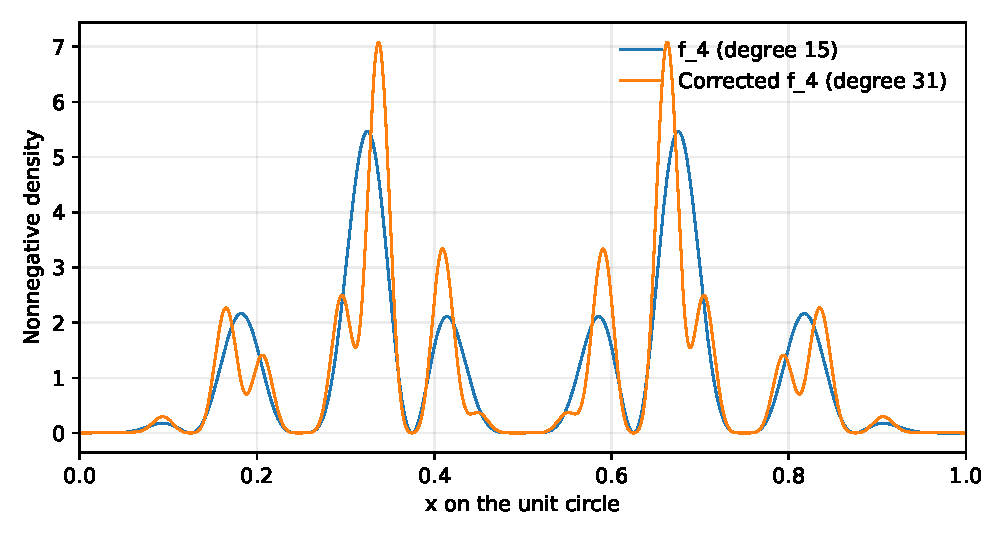
\includegraphics[width=0.94\textwidth]{figures/bc_positive_density.pdf}
\caption{The raw and corrected densities at $m=4$. Both are nonnegative.
The corrected curve reproduces the limiting measure's Fourier coefficients
through $|k|=16$ exactly. The figure makes no assertion of pointwise convergence
to a density of the limit.}
\label{bc:fig:density}
\end{figure}

\section{Smooth and analytic observables}
For $r\ge0$, write
\begin{equation}
 \Ast_r(\phi)=\sum_{k\in\Z\setminus\{0\}}|k|^r|\widehat\phi(k)|.
 \label{bc:eq:wiener}
\end{equation}
Every smooth periodic function has finite $\Ast_r$ for every fixed $r$: repeated
integration by parts bounds its Fourier coefficients by any desired power.

\begin{corollary}[Tail-only integration error]
\label{bc:cor:observable}
For an absolutely convergent Fourier series,
\begin{equation}
 \abs{\pair{\mt_m-\mu}{\phi}}
 \le2\sum_{|k|>N}|\widehat\phi(k)|.
 \label{bc:eq:observable-tail}
\end{equation}
Consequently, whenever $\Ast_r(\phi)<\infty$,
\begin{equation}
 \abs{\pair{\mt_m-\mu}{\phi}}\le2N^{-r}\Ast_r(\phi).
 \label{bc:eq:observable-power}
\end{equation}
If $|\widehat\phi(k)|\le M\rho^{|k|}$ for $0<\rho<1$, then
\begin{equation}
 \abs{\pair{\mt_m-\mu}{\phi}}
 \le\frac{4M\rho^{N+1}}{1-\rho}.
 \label{bc:eq:observable-exp}
\end{equation}
\end{corollary}
\begin{proof}
Termwise pairing is justified by absolute convergence and finite total variation.
Every coefficient on the low band vanishes by~\eqref{bc:eq:band-exact}; every other
coefficient of the difference has magnitude at most two because both measures
are probabilities. Summing the Fourier tail gives~\eqref{bc:eq:observable-tail};
comparison with $|k|^r/N^r$ and a geometric series gives the other two statements.
\end{proof}

For a fixed $C^\infty$ observable, the corrected error decays faster than every
power of $N^{-1}$. For a fixed analytic strip it decays exponentially in $N$.
The constants depend on the observable or the strip, so these statements must
not be applied uniformly to probes whose frequencies grow with $N$.

\begin{remark}[Why positivity is a genuine constraint]
Ordinary Richardson extrapolation often uses a negative weight. Here the raw
error alternates in $m$, so the extrapolation weights are both positive. It is
therefore exact on an expanding spectral band without sacrificing the measure
interpretation. This does not imply convergence in total variation: since $\mu$
is singular and each $\mt_m$ is absolutely continuous, their total-variation norm
distance is two, or one under the convention $\sup_A|\mt_m(A)-\mu(A)|$.
\end{remark}
% ---- BC lines 563--618 ----
\chapter{The universal first correction is a distribution, not a measure}
\label{bc:sec:distribution}

\begin{definition}
Let $\nu$ be the real even periodic distribution specified by
\begin{equation}
 \widehat\nu(0)=0,\qquad
 \widehat\nu(k)=\frac13g(|k|)\quad(k\ne0).
 \label{bc:eq:nu}
\end{equation}
\end{definition}
The bound $|g(k)|\le k$ makes this definition legitimate: pairing its Fourier
coefficients with those of a smooth function is absolutely convergent and
continuous in an appropriate smooth seminorm.

\begin{theorem}[One algebraic correction, with a rapidly small weak remainder]
\label{bc:thm:distribution}
There are distributions $R_m$ such that
\begin{equation}
 \mu_m=\mu+\frac{(-1)^m}{N}\nu+R_m,
 \qquad \widehat R_m(k)=0\quad(|k|\le N).
 \label{bc:eq:distribution-expansion}
\end{equation}
For $r\ge1$ and $\Ast_r(\phi)<\infty$,
\begin{equation}
 \abs{\pair{R_m}{\phi}}\le\frac43N^{-r}\Ast_r(\phi).
 \label{bc:eq:R-bound}
\end{equation}
In particular $(-1)^mN(\mu_m-\mu)\to\nu$ in the space of periodic distributions.
The distribution $\nu$ is not a finite signed measure.
\end{theorem}
\begin{proof}
Define $R_m$ by~\eqref{bc:eq:distribution-expansion}. The low coefficients vanish
by Theorem~\ref{bc:thm:boundary}. For $|k|>N$ the finite product has no coefficient,
so
\[
 \widehat R_m(k)=-\eta(|k|)-\frac{(-1)^m}{3N}g(|k|).
\]
Its magnitude is at most $1+|k|/(3N)\le4|k|/(3N)$. Hence
\[
 |\pair{R_m}{\phi}|
 \le\frac4{3N}\sum_{|k|>N}|k||\widehat\phi(k)|
 \le\frac43N^{-r}\Ast_r(\phi),
\]
where $|k|\le N^{1-r}|k|^r$ on this tail. Taking any fixed $r>1$ proves the
renormalized distributional convergence. Finally
$|\widehat\nu(2^j)|=2^j/3\to\infty$. Fourier coefficients of a finite signed
measure are bounded by its total variation, so $\nu$ cannot be one.
\end{proof}

For each fixed smooth observable the expansion has just one nonzero algebraic
finite-size term. All subsequent powers can be assigned zero coefficients, with
a remainder smaller than every prescribed power. This is a weak statement, not
a pointwise expansion of $f_m$. The negative Sobolev spaces in
Section~\ref{bc:sec:sobolev} quantify exactly how much smoothness is required to
promote it to norm convergence.
% ---- BC lines 620--788 ----
\chapter{An exact analytic factorization of all remaining modes}
\label{bc:sec:analytic}

\section{The affine Mahler equation and its homogeneous defect}
Define the one-sided Fourier generating functions
\begin{equation}
 \mathcal G(z)=\sum_{k=0}^{\infty}\eta(k)z^k,\qquad
 \mathcal G_m(z)=\sum_{k=0}^{N-1}r_m(k)z^k,\qquad |z|<1.
 \label{bc:eq:H}
\end{equation}
These are not the same functions as $E$ and $P_m$: $E$ and $P_m$ encode the
sign sequence, while $\mathcal G$ and $\mathcal G_m$ encode autocorrelations.

\begin{lemma}[Affine functional equations]
\label{bc:lem:MahlerH}
Writing $A(z)=1-(z+z^{-1})/2=-(1-z)^2/(2z)$, one has
\begin{equation}
 \mathcal G(z)=A(z)\mathcal G(z^2)+\frac1{2z},\qquad
 \mathcal G_{m+1}(z)=A(z)\mathcal G_m(z^2)+\frac1{2z}.
 \label{bc:eq:H-Mahler}
\end{equation}
The singularities displayed at zero are removable.
\end{lemma}
\begin{proof}
The even part of either series is the previous series at $z^2$. The odd part is
\[
 -\frac z2\left(\mathcal G(z^2)+\frac{\mathcal G(z^2)-1}{z^2}\right)
\]
for the limiting series, and the identical expression with $\mathcal G_m$ for a finite
one. Adding the even part proves the equations. The constant coefficient is
one on both sides, which also exhibits the cancellation at zero.
\end{proof}

\begin{theorem}[Exact analytic defect]
\label{bc:thm:analytic}
The function
\begin{equation}
 \mathcal K(w)=\frac{3(1-\mathcal G(w))}{wE(w)^2},\qquad \mathcal K(0)=1,
 \label{bc:eq:K}
\end{equation}
is analytic on $\mathbb D$. For every $m\ge0$ and $z\in\mathbb D$,
\begin{equation}
 \boxed{\quad \mathcal G_m(z)-\mathcal G(z)
 =\frac{(-1)^m}{3N}\,zE(z)^2\mathcal K(z^N).\quad}
 \label{bc:eq:analytic-defect}
\end{equation}
If $\Ht_m=(\mathcal G_m+2\mathcal G_{m+1})/3$, then
\begin{equation}
 \Ht_m(z)-\mathcal G(z)
 =\frac{(-1)^m}{9N}\,zE(z)^2
       \bigl(\mathcal K(z^N)-\mathcal K(z^{2N})\bigr).
 \label{bc:eq:analytic-corrected}
\end{equation}
\end{theorem}
\begin{proof}
Subtract the two equations in~\eqref{bc:eq:H-Mahler}. Iterating the resulting
homogeneous equation from $\mathcal G_0=1$ gives
\begin{align*}
 \mathcal G_m(z)-\mathcal G(z)
 &=\left(\prod_{j=0}^{m-1}A(z^{2^j})\right)(1-\mathcal G(z^N))\\
 &=\frac{(-1)^m}{N}z^{1-N}P_m(z)^2(1-\mathcal G(z^N)).
\end{align*}
The infinite product splits as $E(z)=P_m(z)E(z^N)$. Substitute
$1-\mathcal G(w)=wE(w)^2\mathcal K(w)/3$ to obtain~\eqref{bc:eq:analytic-defect}.
The denominator in~\eqref{bc:eq:K} has no zeros except its explicit first-order
zero at zero, while $1-\mathcal G(w)=w/3+O(w^2)$, so $\mathcal K$ is analytic and $\mathcal K(0)=1$.
Combining two consecutive levels gives~\eqref{bc:eq:analytic-corrected}.
\end{proof}

The proof also supplies a second derivation of the low-band theorem: in
$\mathcal Q(z)\mathcal K(z^N)$, the nonconstant terms of $\mathcal K$ can contribute only from degree $N+1$
onward. The exact boundary correction is precisely the constant term $\mathcal K(0)=1$.

\section{Two-colored binary partitions and positive defect coefficients}
Let $p_2(n)$ count partitions of $n$ into powers of two, with each part available
in two distinguishable colors. Equivalently,
\begin{equation}
 \mathcal P(z)=\frac1{E(z)^2}
 =\prod_{j\ge0}(1-z^{2^j})^{-2}
 =\sum_{n\ge0}p_2(n)z^n.
 \label{bc:eq:binary-partitions}
\end{equation}
This product converges locally uniformly on the disk. The combinatorial
interpretation follows by assigning independently a nonnegative multiplicity to
each color of each power of two.

\begin{theorem}[Finite coefficient formula and positivity]
\label{bc:thm:K-coeff}
The analytic function $\mathcal K$ satisfies
\begin{equation}
 2\mathcal K(z)+\mathcal K(z^2)=3\mathcal P(z).
 \label{bc:eq:K-Mahler}
\end{equation}
Writing $\mathcal K(z)=\sum_{n\ge0}\kappa_nz^n$, one has $\kappa_0=1$ and, for $n\ge1$,
\begin{equation}
 \boxed{\quad
 \kappa_n=\frac32\sum_{j=0}^{\vnu(n)}
       \left(-\frac12\right)^j p_2(n/2^j).
 \quad}
 \label{bc:eq:kappa-finite}
\end{equation}
All $\kappa_n$ are positive, and
\begin{equation}
 \frac34p_2(n)\le\kappa_n\le\frac32p_2(n)\qquad(n\ge1).
 \label{bc:eq:kappa-bounds}
\end{equation}
\end{theorem}
\begin{proof}
From~\eqref{bc:eq:H-Mahler},
\[
 1-\mathcal G(z)=A(z)(1-\mathcal G(z^2))+\frac z2.
\]
Using $E(z)=(1-z)E(z^2)$ and the definition of $\mathcal K$ transforms this into
$\mathcal K(z)=3/(2E(z)^2)-\mathcal K(z^2)/2$, proving~\eqref{bc:eq:K-Mahler}.
Comparison of coefficients gives
\[
 2\kappa_n+\mathbf1_{2\mid n}\kappa_{n/2}=3p_2(n)\quad(n\ge1).
\]
The descending recursion ends at an odd integer; expanding it proves the finite
formula. Adding a part of size one of a fixed color is an injection from the
partitions of $n$ into those of $n+1$, so $p_2(n)$ is nondecreasing. In the
alternating finite sum the magnitude of each term is at most half that of the
previous term. It lies between its first term minus its second and its first
term. Those bounds, multiplied by $3/2$, yield~\eqref{bc:eq:kappa-bounds}; if the
second term is absent the upper bound is attained.
\end{proof}

For reference, the first coefficients are
\begin{align*}
 (p_2(n))_{n=0}^{8}&=(1,2,5,8,16,24,40,56,88),\\
 (\kappa_n)_{n=0}^{8}&=(1,3,6,12,21,36,54,84,243/2).
\end{align*}
The $\kappa_n$ need not be integers. Their positivity is particularly useful:
an alternating expression involving binary partitions becomes an analytic
function with strictly positive Taylor coefficients.

\begin{corollary}[A convergent finite-size expansion]
\label{bc:cor:transseries}
For $|z|<1$,
\begin{equation}
 \mathcal G_m(z)-\mathcal G(z)
 =\frac{(-1)^m}{3N}\mathcal Q(z)
       \sum_{j=0}^{\infty}\kappa_jz^{jN}.
 \label{bc:eq:lacunary-expansion}
\end{equation}
For fixed $0<r<1$ and $J\ge0$, truncation after $j=J$ has error
$O_{J,r}(N^{-1}r^{(J+1)N})$, uniformly for $|z|\le r$.
The first mode missed by the positive correction is exactly
\begin{equation}
 \widehat{\mt_m}(N+1)-\eta(N+1)=\frac{(-1)^m}{3N}.
 \label{bc:eq:first-missed}
\end{equation}
\end{corollary}
\begin{proof}
Expand the analytic function $\mathcal K$ in~\eqref{bc:eq:analytic-defect}. On $|w|\le r$,
its Taylor remainder after $J$ is bounded by $C_{J,r}|w|^{J+1}$; for example,
factor out that power and use continuity of the resulting analytic remainder
on the compact disk. Put $w=z^N$ and bound $\mathcal Q$ on $|z|\le r$.
Finally $\mathcal Q(z)=z+O(z^2)$, and
$\mathcal K(z^N)-\mathcal K(z^{2N})=3z^N+O(z^{2N})$. Extracting the coefficient of $z^{N+1}$
in~\eqref{bc:eq:analytic-corrected} proves~\eqref{bc:eq:first-missed}.
\end{proof}

This is a convergent analytic expansion in the exponentially small variable
$z^N$, multiplied by the alternating algebraic factor $N^{-1}$. It may be
viewed as a finite-size transseries on compact subsets of the disk. No assertion
of convergence on $|z|=1$, nor an interchange with a boundary limit, is included.
The distinction is essential because the circle supports the singular limiting
measure and the non-measure correction.
% ---- BC lines 790--860 ----
\chapter{Alternating bounds for Poisson observables}
\label{bc:sec:poisson}

For $0<\rho<1$, consider the positive Poisson kernel centered at zero,
\begin{equation}
 \Pi_\rho(x)=\frac{1-\rho^2}{1-2\rho\cos(2\pi x)+\rho^2}
 =1+2\sum_{k\ge1}\rho^k\cos(2\pi kx).
 \label{bc:eq:poisson}
\end{equation}
Its expectation under the limiting measure is $2\mathcal G(\rho)-1$. The positivity
of $\mathcal K$ turns the analytic factorization into a signed, not merely absolute,
error certificate.

\begin{theorem}[Poisson bracketing and strict improvement]
\label{bc:thm:poisson}
For every $m\ge0$, the two errors
$\pair{\mu_m-\mu}{\Pi_\rho}$ and
$\pair{\mt_m-\mu}{\Pi_\rho}$ have sign $(-1)^m$ and are nonzero.
Writing $t=\rho^N$, their ratio is
\begin{equation}
 \frac{\pair{\mt_m-\mu}{\Pi_\rho}}
      {\pair{\mu_m-\mu}{\Pi_\rho}}
 =\frac{\mathcal K(t)-\mathcal K(t^2)}{3\mathcal K(t)}\in(0,1/3).
 \label{bc:eq:poisson-ratio}
\end{equation}
As $m\to\infty$ this ratio is asymptotic to $\rho^N$.
The even raw approximations decrease to the limit and the odd raw approximations
increase to it. Both raw and corrected approximations give upper bounds at even
levels and lower bounds at odd levels.
\end{theorem}
\begin{proof}
For real $\rho\in(0,1)$, $\mathcal Q(\rho)=\rho E(\rho)^2>0$. Theorems
\ref{bc:thm:analytic} and~\ref{bc:thm:K-coeff} give the exact errors
\begin{align}
 \pair{\mu_m-\mu}{\Pi_\rho}
 &=\frac{2(-1)^m}{3N}\mathcal Q(\rho)\mathcal K(t),\label{bc:eq:raw-poisson}\\
 \pair{\mt_m-\mu}{\Pi_\rho}
 &=\frac{2(-1)^m}{9N}\mathcal Q(\rho)\bigl(\mathcal K(t)-\mathcal K(t^2)\bigr).
 \label{bc:eq:corrected-poisson}
\end{align}
Strict positivity of the coefficients implies $\mathcal K(t)>\mathcal K(t^2)>0$. This proves
all sign and ratio statements. Since $\mathcal K(t)=1+3t+O(t^2)$, the ratio equals
$t+O(t^2)$. Finally the magnitude of the raw error at level $m+2$, divided by
that at level $m$, is $\mathcal K(t^4)/(4\mathcal K(t))<1/4$. Its sign is unchanged. This proves
the nesting of each raw parity subsequence.
\end{proof}

The theorem concerns Poisson kernels centered at zero. A spatially shifted kernel
introduces oscillatory phases in its Fourier coefficients, so the same positivity
argument does not automatically provide alternating upper and lower bounds.
Likewise, nesting of the \emph{corrected} parity subsequences is not needed and
is not asserted here.

\begin{table}[tb]
\centering\small
\input{tables/bc_poisson_table.tex}
\caption{Absolute errors for $\Pi_{4/5}$. Values were evaluated with 160-digit
arithmetic from the exact factorizations and independently checked against
finite Laurent coefficients. Rounded decimal values are illustrations, not
interval-arithmetic certificates. The signs are rigorously $(-1)^m$.}
\label{bc:tab:poisson}
\end{table}

\begin{figure}[tb]
\centering
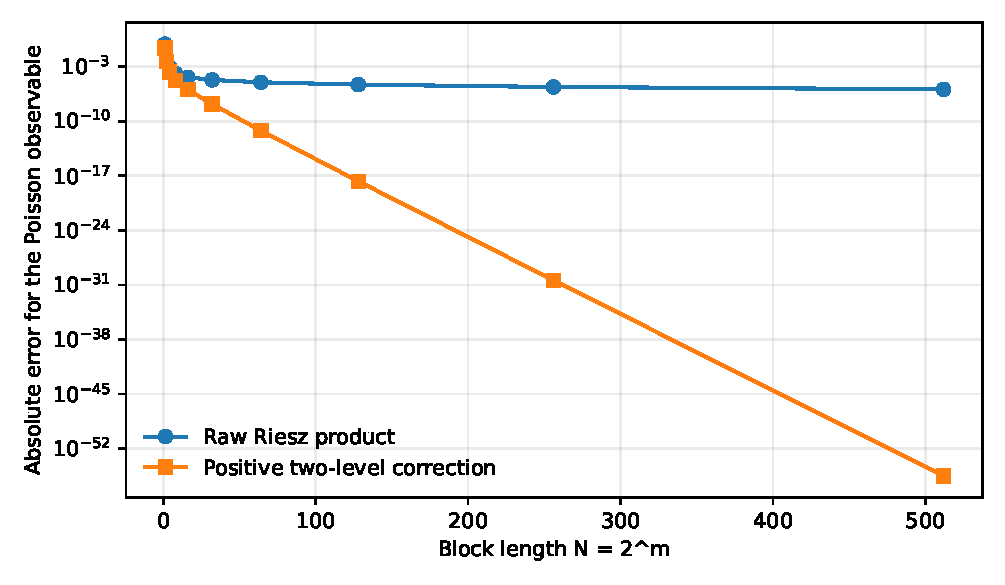
\includegraphics[width=0.94\textwidth]{figures/bc_poisson_convergence.pdf}
\caption{The same Poisson errors. The raw error eventually follows $N^{-1}$;
the corrected error has the additional factor $(4/5)^N$. This dramatic gain is
for a fixed analytic observable, not a claim of total-variation convergence.}
\label{bc:fig:poisson}
\end{figure}
% ---- BC lines 862--998 ----
\chapter{Exact dyadic energies and the classical moment exponent}
\label{bc:sec:energy}

\section{A common two-dimensional transfer matrix}
The growth of $g(k)$ along powers of two alone does not determine its Sobolev
regularity. We need the total squared energy in a dyadic shell. Endpoint-weighted
sums eliminate otherwise distracting boundary terms. Define
\begin{align}
 U_m&=\sum_{k=1}^{N-1}g(k)^2+\frac12g(N)^2,&
 V_m&=\sum_{k=0}^{N-1}g(k)g(k+1),\label{bc:eq:UV}\\
 X_m&=\sum_{k=1}^{N-1}\eta(k)^2+\frac59,&
 Y_m&=\sum_{k=0}^{N-1}\eta(k)\eta(k+1).
 \label{bc:eq:XY}
\end{align}
The constant $5/9$ is the trapezoidal endpoint contribution
$(\eta(0)^2+\eta(N)^2)/2=(1+1/9)/2$.

\begin{proposition}[Exact energy recurrences]
\label{bc:prop:energies}
Let
\begin{equation}
 M=\begin{pmatrix}6&2\\-4&-4\end{pmatrix}.
 \label{bc:eq:M}
\end{equation}
Then
\begin{equation}
 \binom{U_{m+1}}{V_{m+1}}=M\binom{U_m}{V_m},\qquad
 \binom{X_{m+1}}{Y_{m+1}}=\frac14M\binom{X_m}{Y_m},
 \label{bc:eq:energy-matrices}
\end{equation}
with $(U_0,V_0)=(1/2,0)$ and $(X_0,Y_0)=(5/9,-1/3)$.
\end{proposition}
\begin{proof}
For $g$, the even-index contribution to $U_{m+1}$ is $4U_m$, including the
half-weighted endpoint. The odd-index contribution is
\[
 \sum_{r=0}^{N-1}(g(r)+g(r+1))^2=2U_m+2V_m,
\]
because $g(0)=0$. Thus $U_{m+1}=6U_m+2V_m$. Adjacent pairs at the two parities
contribute
\[
 \sum_{r=0}^{N-1}\bigl[-2g(r)(g(r)+g(r+1))
       -2(g(r)+g(r+1))g(r+1)\bigr]
 =-4U_m-4V_m.
\]
This proves the first matrix equation.

For $\eta$, the even contribution to the trapezoidal square sum is $X_m$.
The odd contribution is $(2X_m+2Y_m)/4$, giving
$X_{m+1}=(3X_m+Y_m)/2$. The adjacent-pair sum is
$-(2X_m+2Y_m)/2=-X_m-Y_m$. This is precisely $M/4$.
The initial values follow from $N=1$, $g(1)=1$, and $\eta(1)=-1/3$.
\end{proof}

\begin{corollary}[Closed forms]
\label{bc:cor:energy-closed}
Put $d=\sqrt{17}$, $\Lambda=1+d$, and $q=\Lambda/4$. Then
\begin{align}
 U_m&=\frac{5+d}{4d}\Lambda^m
      +\frac{d-5}{4d}(1-d)^m,\label{bc:eq:U-closed}\\
 X_m&=\frac{19+5d}{18d}q^m
      +\frac{5d-19}{18d}\left(\frac{1-d}{4}\right)^m.
 \label{bc:eq:X-closed}
\end{align}
In particular, $U_m\asymp\Lambda^m$ and $X_m\asymp q^m$.
\end{corollary}
\begin{proof}
The characteristic polynomial of $M$ is $t^2-2t-16$. Hence
$U_{m+2}=2U_{m+1}+16U_m$ with $U_0=1/2$, $U_1=3$.
For $M/4$ it is $t^2-t/2-1$, and $X_0=5/9$, $X_1=2/3$.
Solving these second-order recurrences gives the displayed formulas. The
coefficients of the dominant positive roots are positive and the other roots
have smaller modulus, proving the comparisons.
\end{proof}

For clarity about prior work, $\sum_{k=0}^{N-1}\eta(k)^2=X_m+4/9$ is the
square-correlation formula recorded in~\cite{cmps}. It is not a new exponent
calculation. What matters here is that the boundary sequence has the \emph{same}
energy matrix, without the factor $1/4$.

\section{The fourth moment as a Stern energy}
\begin{proposition}
\label{bc:prop:fourth}
For $N=2^m$,
\begin{equation}
 \int_0^1|P_m(\ee^{2\pi\ii x})|^4\dd x=2U_m,
 \qquad \norm{f_m}_{L^2}^2=\frac{2U_m}{N^2}.
 \label{bc:eq:fourth}
\end{equation}
\end{proposition}
\begin{proof}
The coefficients of $P_m(z)^2$ through degree $N-1$ equal
$g(1),\ldots,g(N)$, since truncating $E$ at degree $N-1$ cannot change these
convolution coefficients. The reflection identity
$z^{N-1}P_m(z^{-1})=(-1)^mP_m(z)$ makes $P_m^2$ palindromic. Its coefficient
squares therefore sum to
$2\sum_{k=1}^{N-1}g(k)^2+g(N)^2=2U_m$. Parseval applied to $P_m^2$ proves the
first equation, and division by $N^2$ proves the second.
\end{proof}

This connects our transfer calculation to the classical even-moment setting
of~\cite{mmr}. It also avoids numerical integration of highly oscillatory products.

\section{Dyadic shell estimates}
Define
\begin{equation}
 \sigma=\frac12\log_2\frac{1+\sqrt{17}}4
       =0.178509318430288\ldots,\qquad
 s_* = 1+\sigma=1.178509318430288\ldots.
 \label{bc:eq:exponents}
\end{equation}
The familiar correlation dimension is $D_2=1-2\sigma
=3-\log_2(1+\sqrt{17})$~\cite{zaks}. We will use only the energy estimates,
not a new dimension theorem.

\begin{lemma}[Two-sided shell energies]
\label{bc:lem:shell}
With $N=2^m$, constants independent of $m$ give
\begin{equation}
 \sum_{N<k\le2N}g(k)^2\asymp N^{2s_*},\qquad
 \sum_{N<k\le2N}\eta(k)^2\asymp N^{2\sigma}.
 \label{bc:eq:shells}
\end{equation}
\end{lemma}
\begin{proof}
Let $G_m=\sum_{k=1}^Ng(k)^2=U_m+4^m/2$.
Then the first shell sum is
$G_{m+1}-G_m=U_{m+1}-U_m+3\cdot4^m/2$.
Since $\Lambda>4$ and the dominant coefficient in~\eqref{bc:eq:U-closed} is
positive, this is a positive constant times $\Lambda^m$ asymptotically.
The remaining finitely many shells have positive energy, so constants can be
adjusted to cover them all. For $\eta$, the corresponding prefix sum through
$N$ is $X_m-4/9$. Its shell difference is $X_{m+1}-X_m$, asymptotic to a
positive constant times $q^m$, since $q>1$. Each shell contains a power of two,
where $\eta=-1/3$, so again every finite initial shell is nonzero. Finally
$\Lambda^m=N^{2s_*}$ and $q^m=N^{2\sigma}$.
\end{proof}
% ---- BC lines 1000--1182 ----
\chapter{Sharp Sobolev regularity and finite-size convergence}
\label{bc:sec:sobolev}

\section{The function spaces and a shell-summation lemma}
For a periodic distribution $u$, use the norm
\begin{equation}
 \norm{u}_{H^{-s}}^2=
 \sum_{k\in\Z}(1+k^2)^{-s}|\widehat u(k)|^2.
 \label{bc:eq:Sobolev}
\end{equation}
The use of $k$ rather than $2\pi k$ fixes constants but not thresholds. A pairing
with $\phi\in H^s$ is bounded by $\norm{u}_{H^{-s}}\norm{\phi}_{H^s}$.

\begin{lemma}[Weighted dyadic sums]
\label{bc:lem:weighted}
Suppose $a_k\ge0$ and
$\sum_{2^j<k\le2^{j+1}}a_k\asymp2^{2tj}$, with a nonzero fixed low coefficient.
For $N=2^m$ and $s>t$,
\begin{equation}
 \sum_{k>N}(1+k^2)^{-s}a_k\asymp N^{2(t-s)}.
 \label{bc:eq:weighted-tail}
\end{equation}
The full weighted series converges if and only if $s>t$. Moreover, for positive
$s$ the prefix sum through $N$ is, as $N\to\infty$,
\begin{equation}
 \sum_{1\le k\le N}(1+k^2)^{-s}a_k\asymp
 \begin{cases}
 N^{2(t-s)},&s<t,\\
 \log N,&s=t,\\
 1,&s>t.
 \end{cases}
 \label{bc:eq:weighted-prefix}
\end{equation}
\end{lemma}
\begin{proof}
On the $j$th shell, the weight is comparable to $2^{-2sj}$, with comparison
constants depending only on $s$. The shell's weighted contribution is therefore
comparable to $2^{2(t-s)j}$. Summing this geometric progression over $j\ge m$
gives~\eqref{bc:eq:weighted-tail}; convergence fails at equality because each shell
then contributes a positive amount. Summing over $j<m$ gives respectively a
last-term-dominated progression, $m$ comparable summands, or a bounded convergent
series. The nonzero low coefficient gives the last case's positive lower bound.
\end{proof}

\begin{theorem}[Exact regularity thresholds]
\label{bc:thm:regularity}
The limiting measure and its boundary correction satisfy
\begin{equation}
 \mu\in H^{-s}\ \Longleftrightarrow\ s>\sigma,
 \qquad
 \nu\in H^{-s}\ \Longleftrightarrow\ s>s_*.
 \label{bc:eq:regularity}
\end{equation}
Neither endpoint is included.
\end{theorem}
\begin{proof}
Apply Lemma~\ref{bc:lem:weighted} to the two shell estimates in
Lemma~\ref{bc:lem:shell}. Evenness duplicates the positive frequencies, and the
constant Fourier coefficient does not affect convergence. The factor $1/3$
in $\widehat\nu$ changes only the norm constant.
\end{proof}

The difference of exactly one in the thresholds expresses a genuine derivative's
worth of additional roughness in the universal correction. It is compatible with,
but substantially more precise than, the pointwise bound $|g(k)|\le k$.

\section{Norm convergence of the renormalized error}
\begin{theorem}[Sharp topology for the first correction]
\label{bc:thm:renormalized}
Set $Z_m=(-1)^mN(\mu_m-\mu)$. Then
\begin{equation}
 Z_m\longrightarrow\nu\quad\hbox{in }H^{-s}
 \quad\Longleftrightarrow\quad s>s_*.
 \label{bc:eq:Z-limit}
\end{equation}
For $s>s_*$,
\begin{equation}
 \norm{Z_m-\nu}_{H^{-s}}\ll_s N^{s_*-s}.
 \label{bc:eq:Z-rate}
\end{equation}
\end{theorem}
\begin{proof}
On $|k|\le N$ the difference vanishes. On the complement it equals
$-(-1)^mN\eta(|k|)-g(|k|)/3$. The squared norm is bounded by a fixed constant
times the sum of $N^2$ times the $\eta$ tail energy and the $g$ tail energy.
By~\eqref{bc:eq:weighted-tail}, both have size at most $N^{2(s_*-s)}$.
This proves the norm bound and convergence. Conversely, a norm limit in
$H^{-s}$ must have every Fourier coefficient equal to the eventually exact
coefficient $g(|k|)/3$, hence must be $\nu$. That distribution belongs to
$H^{-s}$ only for $s>s_*$. For $s\le\sigma$, already $\mu_m-\mu$ is not an
element of $H^{-s}$; the finite polynomial cannot remove the divergent tail.
\end{proof}

\section{The raw approximation: a phase transition and saturation}
\begin{theorem}[Sharp raw error rates]
\label{bc:thm:raw-rate}
For every fixed $s>\sigma$, as $N=2^m\to\infty$,
\begin{equation}
 \boxed{\quad
 \norm{\mu_m-\mu}_{H^{-s}}\asymp_s
 \begin{cases}
 N^{\sigma-s},&\sigma<s<s_*,\\
 N^{-1}\sqrt{\log N},&s=s_*,\\
 N^{-1},&s>s_*.
 \end{cases}\quad}
 \label{bc:eq:raw-rates}
\end{equation}
For $s>s_*$ there is also the exact leading norm limit
\begin{equation}
 N\norm{\mu_m-\mu}_{H^{-s}}\longrightarrow\norm{\nu}_{H^{-s}}>0.
 \label{bc:eq:raw-leading-norm}
\end{equation}
\end{theorem}
\begin{proof}
Because the finite coefficients vanish beyond their support, the squared norm
has the exact decomposition
\begin{equation}
 \norm{\mu_m-\mu}_{H^{-s}}^2
 =\frac{2}{9N^2}\sum_{k=1}^{N}(1+k^2)^{-s}g(k)^2
   +2\sum_{k>N}(1+k^2)^{-s}\eta(k)^2.
 \label{bc:eq:exact-norm-decomposition}
\end{equation}
The endpoint $k=N$ is included in the first sum by Theorem~\ref{bc:thm:boundary}.
Use~\eqref{bc:eq:weighted-prefix} with $t=s_*$ for the first term and
\eqref{bc:eq:weighted-tail} with $t=\sigma$ for the second. If $s<s_*$, both are
of order $N^{2(\sigma-s)}$. At $s=s_*$ the first is of order
$N^{-2}\log N$, while the second is of order $N^{-2}$. Above $s_*$ the first
is of order $N^{-2}$ and the second is smaller. Taking square roots proves the
three regimes. Equation~\eqref{bc:eq:raw-leading-norm} follows from
Theorem~\ref{bc:thm:renormalized} and continuity of the norm; $\nu\ne0$ because
its first coefficient is $1/3$.
\end{proof}

Thus additional smoothness ceases to improve the raw rate after $s_*$. The
obstruction is not an estimate artifact: it is a specific nonzero distribution,
with an exactly known Fourier series.

\section{The corrected approximation removes saturation}
\begin{theorem}[Sharp corrected rate and bandwidth optimality]
\label{bc:thm:corrected-rate}
For every fixed $s>\sigma$,
\begin{equation}
 \boxed{\quad
 \norm{\mt_m-\mu}_{H^{-s}}\asymp_s N^{\sigma-s}.
 \quad}
 \label{bc:eq:corrected-rates}
\end{equation}
More generally, fix $C>0$. Every approximant $v_N$ whose Fourier support is
contained in $|k|\le CN$ satisfies, for all sufficiently large dyadic $N$,
\begin{equation}
 \norm{v_N-\mu}_{H^{-s}}\ge c_{s,C}N^{\sigma-s}.
 \label{bc:eq:bandwidth-lower}
\end{equation}
No positivity assumption on $v_N$ is required for this lower bound.
\end{theorem}
\begin{proof}
The corrected error vanishes through $N$. For the middle band $N<|k|<2N$,
use $(1+k^2)^{-s}\le N^{-2s}$ and
$|a-b|^2\le2|a|^2+2|b|^2$. By~\eqref{bc:eq:positive-density} and Parseval,
\[
 \sum_k|\widehat{\mt_m}(k)|^2
 =\norm{\ft_m}_{L^2}^2
 \le\frac{25}{9}\norm{f_m}_{L^2}^2
 =\frac{50U_m}{9N^2}\ll N^{2\sigma}.
\]
The $\eta$ energy on the middle band has the same upper order by
Lemma~\ref{bc:lem:shell}. Thus that band's weighted contribution is
$O_s(N^{2(\sigma-s)})$. Beyond $2N$ the approximant has no coefficients, and
Lemma~\ref{bc:lem:weighted} gives the same order for the tail. This proves the
upper bound. The unchanged $\eta$ tail beyond $2N$ alone proves the matching
lower bound.

For the general assertion, choose a fixed integer $j$ with $2^j>C$ and take the
shell $2^jN<|k|\le2^{j+1}N$. All coefficients of $v_N$ there vanish. Its
weighted $\eta$ energy is bounded below by a constant times
$N^{2(\sigma-s)}$. Taking a square root proves~\eqref{bc:eq:bandwidth-lower}.
\end{proof}

For rough admissible tests, $\sigma<s<s_*$, the correction improves the constant
and exactness band but cannot improve the order dictated by the unresolved
spectral tail. At the threshold it removes $\sqrt{\log N}$, and above the
threshold it removes the $N^{-1}$ saturation completely. These are different
regimes of a single exact identity, rather than competing convergence claims.
% ---- BC lines 1184--1416 ----
\chapter{A parameter family and the sharp positivity threshold}
\label{bc:sec:parameter}

\section{Amplitude-deformed binary Riesz products}
For $-1\le a\le1$, define
\begin{equation}
 f_m^{(a)}(x)=\prod_{j=0}^{m-1}(1-a\cos(2\pi2^jx)),\qquad
 \mu_m^{(a)}=f_m^{(a)}(x)\dd x.
 \label{bc:eq:parameter-product}
\end{equation}
These are amplitude deformations; no identification with a differently
parameterized phase-deformation family is intended. Every factor is nonnegative.
The constant coefficient remains one: in
$f_{m+1}^{(a)}=(1-a\cos(2\pi x))f_m^{(a)}(2x)$, the last factor has only even
frequencies. Hence all $\mu_m^{(a)}$ are probabilities. Their Fourier recursion is
\begin{equation}
 r_{m+1}^{(a)}(2r)=r_m^{(a)}(r),\qquad
 r_{m+1}^{(a)}(2r+1)=-\frac a2\bigl(r_m^{(a)}(r)+r_m^{(a)}(r+1)\bigr).
 \label{bc:eq:parameter-rec}
\end{equation}
The same fixed-index induction as in Proposition~\ref{bc:prop:limit} proves a weak
limit $\mu^{(a)}$, whose coefficients $\eta_a$ obey this recursion with
\begin{equation}
 \eta_a(0)=1,\qquad \eta_a(1)=-\frac a{2+a}.
 \label{bc:eq:parameter-eta}
\end{equation}
The coefficient bound $|\eta_a(k)|\le1$ follows from the probability measure.

When $a=0$, every measure is Lebesgue measure. When $a=1$, we recover the
Thue--Morse case. At $a=-1$,
\begin{equation}
 f_m^{(-1)}(x)=\frac1N\left|\sum_{n=0}^{N-1}\ee^{2\pi\ii nx}\right|^2,
 \label{bc:eq:Fejer}
\end{equation}
the dyadic Fej\'er kernel; its coefficients tend to one, so its limit is the point
mass at zero. This endpoint is a useful exact check on the general formulas.

\begin{theorem}[Parameterized Stern boundary]
\label{bc:thm:parameter-boundary}
Fix $a\in[-1,1]\setminus\{0\}$, and write
\begin{equation}
 \alpha=-\frac a2,\qquad c=\frac a{2+a},\qquad
 g_a(k)=B_k(-2/a).
 \label{bc:eq:parameter-g}
\end{equation}
Then, exactly for $0\le k\le N=2^m$,
\begin{equation}
 r_m^{(a)}(k)-\eta_a(k)=c\alpha^m g_a(k).
 \label{bc:eq:parameter-boundary}
\end{equation}
\end{theorem}
\begin{proof}
The initial coefficient at $k=1$ has error $c$, agreeing with $g_a(1)=1$.
The even recursion for $g_a$ multiplies by $-2/a=\alpha^{-1}$, compensating for
the extra $\alpha$ at the next level. Its odd recursion is the sum of two
adjacent values, exactly matching the factor $\alpha$ in the Fourier recursion.
The induction of Theorem~\ref{bc:thm:boundary}, with these constants substituted,
therefore proves the statement, including the endpoint.
\end{proof}

\begin{theorem}[Exactness and a sharp positivity interval]
\label{bc:thm:parameter-positive}
For $a\in[-1,1]$, put
\begin{equation}
 \mt_m^{(a)}=\frac{a\mu_m^{(a)}+2\mu_{m+1}^{(a)}}{2+a}.
 \label{bc:eq:parameter-correction}
\end{equation}
It has total mass one and agrees with $\mu^{(a)}$ at every Fourier mode
$|k|\le N$. Its density is
\begin{equation}
 \ft_m^{(a)}(x)=f_m^{(a)}(x)
     \left(1-\frac{2a}{2+a}\cos(2\pi Nx)\right).
 \label{bc:eq:parameter-density}
\end{equation}
For every $m$, this density is nonnegative on the whole circle if and only if
\begin{equation}
 \boxed{\qquad -\frac23\le a\le1.\qquad}
 \label{bc:eq:positivity-threshold}
\end{equation}
For $a\ne0$, the affine combination is uniquely determined by exactness at the
first mode. At $a=0$ all levels coincide and uniqueness is not asserted.
\end{theorem}
\begin{proof}
For $a\ne0$, the common-band errors have ratio $\alpha=-a/2$. Their cancellation
condition is $w+(1-w)\alpha=0$, giving $w=a/(2+a)$. The density identity follows
by factoring $f_{m+1}^{(a)}=f_m^{(a)}(1-a\cos(2\pi Nx))$. The second factor is
nonnegative exactly when $|2a/(2+a)|\le1$, which on $[-1,1]$ is $a\ge-2/3$.
This condition is sufficient since $f_m^{(a)}\ge0$. If $a<-2/3$, the second
factor is negative where $\cos(2\pi Nx)=-1$, for example at $x=1/(2N)$:
its value there is $(2+3a)/(2+a)<0$. Every factor of $f_m^{(a)}$ at this point
is strictly positive, since for $j<m$,
$0<2\pi2^jx\le\pi/2$ and $1-a\cos(2\pi2^jx)\ge1$.
Thus the corrected density is strictly negative on a neighborhood of this point.
This proves necessity,
including the endpoint $a=-1$. The case $a=0$ is immediate.
\end{proof}

\begin{remark}[Negative weights need not force a negative density]
For $-2/3\le a<0$, the coefficient of $\mu_m^{(a)}$ in the affine combination
is negative, yet the resulting density is nonnegative. The factorization, rather
than the signs of the mixing weights alone, decides positivity. Below $-2/3$
this exact two-level construction genuinely becomes signed. The theorem is a
sharp threshold for this construction, not a no-go theorem for every possible
positive approximation with a larger number of levels.
\end{remark}

\section{The full fixed-parameter Sobolev rate law}
The same mechanism has a continuous family of exponents. The proof is included
because the amplitude deformation separates two roles that coincide at $a=1$:
the boundary's geometric decay factor and the limiting measure's energy growth.
Set
\begin{align}
 T_a&=1-a+\frac{a^2}{2},&
 \rho_a&=\frac{T_a+\sqrt{T_a^2+4a}}2,\label{bc:eq:rhoa}\\
 \beta_a&=\log_2\frac2{|a|},&
 \sigma_a&=\frac12\log_2\rho_a,& s_a&=\sigma_a+\beta_a.
 \label{bc:eq:param-exponents}
\end{align}
These quantities are defined for fixed $a\ne0$ in $[-1,1]$.

\begin{theorem}[Parameterized regularity and sharp rates]
\label{bc:thm:parameter-rates}
Let $\widehat\nu_a(0)=0$ and
$\widehat\nu_a(k)=c\,g_a(|k|)$ for $k\ne0$, with $c$ as
in~\eqref{bc:eq:parameter-g}. Then
\begin{equation}
 \mu^{(a)}\in H^{-s}\ \Longleftrightarrow\ s>\sigma_a,
 \qquad \nu_a\in H^{-s}\ \Longleftrightarrow\ s>s_a.
 \label{bc:eq:param-reg}
\end{equation}
For every fixed $s>\sigma_a$,
\begin{align}
 \norm{\mu_m^{(a)}-\mu^{(a)}}_{H^{-s}}
 &\asymp_{a,s}
 \begin{cases}
 N^{\sigma_a-s},&\sigma_a<s<s_a,\\
 N^{-\beta_a}\sqrt{\log N},&s=s_a,\\
 N^{-\beta_a},&s>s_a,
 \end{cases}\label{bc:eq:param-raw}\\
 \norm{\mt_m^{(a)}-\mu^{(a)}}_{H^{-s}}
 &\asymp_{a,s}N^{\sigma_a-s}.
 \label{bc:eq:param-corrected}
\end{align}
The corrected estimate remains valid below the positivity threshold, where the
approximants are signed. For $s>s_a$, the renormalized errors converge to
$\nu_a$ in $H^{-s}$ after multiplication by $\alpha^{-m}$, with error
$O_{a,s}(N^{s_a-s})$.
\end{theorem}
\begin{proof}
Put $b=-2/a$ and define trapezoidal energies
\begin{align*}
 U_m^{(a)}&=\sum_{k=1}^{N-1}g_a(k)^2+\tfrac12g_a(N)^2,&
 V_m^{(a)}&=\sum_{k=0}^{N-1}g_a(k)g_a(k+1),\\
 X_m^{(a)}&=\sum_{k=1}^{N-1}\eta_a(k)^2+\tfrac12(1+c^2),&
 Y_m^{(a)}&=\sum_{k=0}^{N-1}\eta_a(k)\eta_a(k+1).
\end{align*}
The same even-odd splitting used in Proposition~\ref{bc:prop:energies} gives
\begin{equation}
 \binom{X_{m+1}^{(a)}}{Y_{m+1}^{(a)}}=
 M_a\binom{X_m^{(a)}}{Y_m^{(a)}},\qquad
 M_a=\begin{pmatrix}1+a^2/2&a^2/2\\-a&-a\end{pmatrix},
 \label{bc:eq:param-energy}
\end{equation}
and
\begin{equation}
 \binom{U_{m+1}^{(a)}}{V_{m+1}^{(a)}}=
 \begin{pmatrix}b^2+2&2\\2b&2b\end{pmatrix}
 \binom{U_m^{(a)}}{V_m^{(a)}}
 =\frac4{a^2}M_a\binom{U_m^{(a)}}{V_m^{(a)}}.
 \label{bc:eq:param-genergy}
\end{equation}
For example the odd square contribution for $g_a$ is $2U_m^{(a)}+2V_m^{(a)}$;
the adjacent-pair sum is $2b(U_m^{(a)}+V_m^{(a)})$. For $\eta_a$, the odd square
contribution is $a^2(X_m^{(a)}+Y_m^{(a)})/2$, and the adjacent-pair sum is
$-a(X_m^{(a)}+Y_m^{(a)})$. These establish both matrices without omitted
boundary terms.

The characteristic polynomial of $M_a$ is $x^2-T_ax-a$. Its discriminant is
positive. For $a\ge0$ this is immediate. For $a=-u<0$ it is
$(1-u)^2+u^2+u^3+u^4/4>0$. Evaluating the polynomial at one gives $-a^2/2<0$,
so the larger root $\rho_a$ exceeds one. The other root has modulus
$|a|/\rho_a<1$. Thus each first-coordinate energy is a combination of two
distinct real geometric sequences. The coefficient of $\rho_a^m$ in
$X_m^{(a)}$ is strictly positive: otherwise nonnegativity rules out a negative
coefficient, while a zero coefficient would make the energy bounded, contrary
to the $m$ nonzero values $\eta_a(2^j)=-c$ in its prefix.
For $U_m^{(a)}$, the larger eigenvalue is $(4/a^2)\rho_a>b^2$. The coefficient
of that root is again positive: a zero dominant coefficient would contradict
$U_m^{(a)}\ge b^{2m}/2$, because the smaller root has modulus strictly less than
$b^2$.

Consequently, taking differences of prefix energies as in
Lemma~\ref{bc:lem:shell},
\[
 \sum_{N<k\le2N}\eta_a(k)^2\asymp_a N^{2\sigma_a},\qquad
 \sum_{N<k\le2N}g_a(k)^2\asymp_a N^{2s_a}.
\]
The endpoints $g_a(N)^2=b^{2m}$ are lower order than the dominant energy;
the endpoints $\eta_a(N)^2=c^2$ are constant. All finite shells have positive
energy because they contain powers of two. The sequence $g_a$ also has
polynomial growth: $|g_a(k)|\le k^{\beta_a}$ follows by induction from
$|b|=2^{\beta_a}$ and
$r^{\beta_a}+(r+1)^{\beta_a}\le(2r+1)^{\beta_a}$, since $\beta_a\ge1$.
Thus $\nu_a$ is a distribution.

The shell-summation lemma now proves~\eqref{bc:eq:param-reg}. On the low band the
raw error is exactly $c\alpha^mg_a(k)$, with
$|\alpha|^m=N^{-\beta_a}$; outside the support it is $-\eta_a(k)$. Applying
the weighted prefix and tail estimates gives~\eqref{bc:eq:param-raw}, including
the logarithm at the critical exponent. The same tail argument proves the
renormalized convergence and its rate.

For the corrected upper bound, its support is contained in $|k|<2N$ and its
error vanishes through $N$. The low-band identity also gives
\[
 \sum_k|r_m^{(a)}(k)|^2
 \ll_a \sum_{k=0}^{N}\eta_a(k)^2+
        |\alpha|^{2m}\sum_{k=0}^{N}g_a(k)^2
 \ll_a N^{2\sigma_a}.
\]
The multiplicative factor in~\eqref{bc:eq:parameter-density} is bounded in absolute
value by $1+2|a|/(2+a)$. Hence its corrected $L^2$ norm has the same upper order,
even when the factor changes sign. Bounding the middle band and the untouched
tail exactly as in Theorem~\ref{bc:thm:corrected-rate} proves the upper bound in
\eqref{bc:eq:param-corrected}. The tail beyond $2N$ proves the lower bound.
\end{proof}

At $a=-1$, the formulas give $\rho_a=2$, $\sigma_a=1/2$, $\beta_a=1$, and
$s_a=3/2$. Also $g_a(k)=B_k(2)=k$ and $c=-1$, so
$r_m^{(-1)}(k)=1-k/N$ on $0\le k\le N$, the familiar Fej\'er coefficients.
At $a=1$, every formula reduces to the Thue--Morse theorem. The limit $a\to0$
is not uniform in the constants: the case $a=0$ is exactly constant in $m$ and
is correctly excluded from the exponent parametrization.
% ---- BC lines 1418--1525 ----
\chapter{Computation, verification, and proof engineering}
\label{bc:sec:computation}

\section{Exact computation without constructing a large block}
To compute a single stabilized finite Fourier coefficient, choose $m$ with
$2^m\ge k$, compute $\eta(k)$ from its two adjacent-value recursion, compute
$g(k)$ using~\eqref{bc:eq:binary-matrices}, and apply~\eqref{bc:eq:main-boundary}.
The state for $\eta$ has matrices
\begin{equation}
 \binom{\eta(2k)}{\eta(2k+1)}=
 \begin{pmatrix}1&0\\-1/2&-1/2\end{pmatrix}
 \binom{\eta(k)}{\eta(k+1)},\qquad
 \binom{\eta(2k+1)}{\eta(2k+2)}=
 \begin{pmatrix}-1/2&-1/2\\0&1\end{pmatrix}
 \binom{\eta(k)}{\eta(k+1)}.
 \label{bc:eq:eta-binary-matrices}
\end{equation}
Starting from $(\eta(0),\eta(1))=(1,-1/3)$ and reading the bits from most to
least significant takes $O(\log k)$ arithmetic operations. Leading zero bits
leave this initial state unchanged. These are arithmetic-operation counts;
bit complexity also accounts for integer sizes. The signed Stern values have
$O(\log k)$ bits by $|g(k)|\le k$, and the rational recursion for $\eta$ grows
its denominator by at most one factor of two per bit.

When all coefficients through $N$ are required, the descending recurrences can
be tabulated in $O(N)$ arithmetic operations and memory. Directly summing all
correlations takes $O(N^2)$ sign multiplications; an FFT is an alternative for
approximation, but the recurrence plus exact boundary term provides exact
rational coefficients without rounding.

For the analytic correction, the finite formula~\eqref{bc:eq:kappa-finite} uses only
$1+\vnu(n)$ binary partition values. A table of $p_2(0),\ldots,p_2(L)$ can be
computed by a coin-change dynamic program, using two colors of each size
$1,2,4,\ldots$, in $O(L\log L)$ integer additions. Formula~\eqref{bc:eq:K-Mahler}
then computes all $\kappa_n$ in $O(L)$ rational operations. Positivity prevents
large cancellation when evaluating $\mathcal K(t)$ for real $0<t<1$.

\section{Avoiding loss of the corrected error}
At large $N$, directly subtracting two nearly equal high-precision expectations
can lose most significant digits. Equation~\eqref{bc:eq:corrected-poisson} is a
better evaluation formula. Even within that formula, write
\begin{equation}
 \mathcal K(t)-\mathcal K(t^2)=\sum_{j\ge1}\kappa_jt^j(1-t^j),\qquad 0<t<1,
 \label{bc:eq:positive-evaluation}
\end{equation}
instead of subtracting two numbers close to one. Every summand is positive.
For very small $t$, one can factor out $3t$ before accumulating the remaining
series. For complex $z$ or shifted observables this particular positivity is
lost, but the exact disk factorization still applies.

\section{The supplied verification program}
The companion \texttt{verify.py} uses only Python's standard library. Identity
checks use integers and \texttt{fractions.Fraction}; none uses floating-point
equality. The recorded run performs 19,037 checks, including:
\begin{center}
\begin{tabularx}{\textwidth}{@{}p{0.39\textwidth}X@{}}
\toprule
Test family & Range or independent representation \\
\midrule
Aperiodic and forward corrections & Every $0\le k\le2^m$ for $0\le m\le10$. \\
Finite Fourier products & Independent Laurent-polynomial multiplication of all factors. \\
Positive correction and first missed mode & Exact low-band agreement and the coefficient at $N+1$. \\
Signed Stern identity & Direct sign convolution through $k=1024$, bounds, and valuations. \\
Energy transfer and fourth moments & Exact rational sums through level $12$. \\
Analytic factorization & Every coefficient through degree $256$ at levels $0$ through $7$. \\
Partition coefficient formula & Exact coefficients, finite sums, and positivity bounds through $256$. \\
Amplitude family & Nine nonzero rational parameters, every low mode through level $7$, and both energy matrices. \\
\bottomrule
\end{tabularx}
\end{center}
The parameters are $-1,-3/4,-2/3,-1/2,-1/7,1/7,1/4,1/2,1$.
These tests are not replacements for proofs of infinite statements. They check
independent finite representations and are particularly effective at catching
endpoint, sign, normalization, and parameter mistakes.

\texttt{make\_figures.py} separately uses \texttt{mpmath}, \texttt{numpy}, and
\texttt{matplotlib}. The Poisson table uses 160 decimal digits and 2,201 terms
for its independent limiting-series evaluation. The data and the exact test
report are included as JSON. The verification program itself has no dependency
on those optional plotting packages.

\section{Formalization targets in the supplied repository}
No Lean source is supplied or claimed checked here. The following dependency
order isolates relatively small formal targets compatible with the atlas's
existing finite autocorrelation and polynomial-product development.

The first layer is entirely algebraic: define the convolution sequence $g$, prove
its two parity recurrences, identify it with $B_k(-2)$ if a Stern-polynomial
interface is desired, and prove the two exact boundary formulas. The latter
need only natural-number induction, finite sums, binary reflection, and rational
arithmetic. The central low-band cancellation is then a short consequence.

The second layer packages Fourier coefficients of finite trigonometric products.
Positivity of the corrected density is a direct bound on cosine, not a limiting
argument. Weak existence of $\mu$ can be taken from the existing development or
proved from finite coefficient convergence and compactness.

The third layer separates analysis from combinatorics: prove the two energy
matrix identities as finite-sum theorems, solve the scalar recurrences, derive
shell estimates, and then apply an abstract weighted-shell lemma. The sharp
Sobolev thresholds and all three error regimes become applications of that one
lemma to an exact norm decomposition. The analytic factorization is a separate
Mahler-equation branch; its only infinite-product requirements are local uniform
convergence and nonvanishing in the open disk.

This architecture deliberately avoids equating ``proved on paper'' with
``already formalized in the current repository.'' It also keeps classical
spectral-type results out of the dependencies of the new algebraic identities.
% ---- BC lines 1527--1566 ----
\chapter{Further questions suggested by the exact mechanism}
\label{bc:sec:questions}

\section{Non-dyadic windows and binary boundary states}
For a length $L$ that is not a power of two, the finite word decomposes into
signed dyadic blocks. The single correction $g(k)$ should then be replaced by
several cross-boundary states whose coefficients depend on the binary expansion
of $L$. A concrete next problem is to derive a finite-dimensional exact state
system for these defects and determine which subsequences of $L$ admit positive
moment-exact combinations. The present theorems prove the one-state collapse
on dyadic lengths; they do not assert such a collapse for all lengths.

\section{Positive corrections for other substitution spectra}
The general principle is an affine finite Fourier recursion with a contractive
boundary eigenvalue. A negative eigenvalue allows cancellation by positive
weights on two consecutive levels, as in the Thue--Morse case. With several
boundary eigenvalues, the cancellation conditions become a finite moment problem
for the level weights. Determining when these weights, or the resulting density
factor, remain nonnegative is a concrete algebraic question. The interval
$[-2/3,1]$ in the amplitude family shows why positivity of the final factor can
be a less restrictive condition than positivity of every weight.

\section{Distribution functions and nonsmooth local probes}
Theorems~\ref{bc:thm:raw-rate} and~\ref{bc:thm:corrected-rate} describe an entire
Sobolev scale, but they do not automatically settle optimal uniform error for
cumulative distribution functions. Indicator functions are substantially less
smooth than the observables for which the first correction gives a full weak
expansion. A next step is to combine the exact band cancellation with sharp
local mass bounds for the Thue--Morse measure. This requires additional local
information, not another manipulation of the same fixed-mode identity.

\section{More layers versus more exact modes}
Two consecutive products uniquely cancel the one low-band boundary mode.
Three or more levels can cancel selected later analytic sectors in
\eqref{bc:eq:lacunary-expansion}, but the variables at consecutive levels are
$z^N,z^{2N},z^{4N},\ldots$, not ordinary powers of a common mesh parameter.
A useful precise problem is to maximize the exact Fourier band subject to
nonnegative level weights, or more generally a nonnegative factored density.
The first missed coefficient~\eqref{bc:eq:first-missed} supplies the first
nontrivial constraint. No general optimal multi-level scheme is claimed here.
% ---- hand chunk 11-part1-ndhead.tex ----

\chapter{Exact boundary defects for correlations of every order}
\label{nd:sec:correlations}
The Stern boundary term of \cref{bc:thm:boundary} concerns the pair
correlation. The same mechanism, one dyadic block longer than every shift,
controls correlations of every order: a single finite boundary functional,
independent of the block level, gives the exact dyadic defect. Even
correlations have an alternating defect, whereas odd correlations become an
explicit telescoping difference after dyadic blocking, and the same
functional gives formulas for arbitrary numbers of complete blocks without a
recursive correlation hierarchy. The means and their renormalization belong
to the established correlation theory \cite{baake-coons}; the contribution
here is the explicit finite functional, its independence of the level, and
the exact boundary and telescoping formulas. The following elementary
identity replaces an infinite correlation recursion by a finite binary-digit
expression.


% ---- ND lines 228--262 ----
\section{An exact adjacent-correlation sum}
The following elementary identity will replace an infinite correlation
recursion by a finite binary-digit expression.

\begin{definition}
For an integer \(Q=\sum_{j\ge0}b_j2^j\ge0\), define the alternating digit sum
\begin{equation}
 \sigma(Q)=\sum_{j\ge0}(-1)^jb_j.
 \label{nd:eq:sigma}
\end{equation}
In particular, \(\sigma(0)=0\) and \(\sigma(2^k)=(-1)^k\).
\end{definition}

\begin{lemma}[Adjacent correlation at every endpoint]
For every \(Q\ge0\),
\begin{equation}
 C(Q):=\sum_{q=0}^{Q-1}\eps_q\eps_{q+1}
       =-\frac Q3-\frac23\sigma(Q).
 \label{nd:eq:C}
\end{equation}
Consequently \(C(Q)/Q\to-1/3\) as \(Q\to\infty\).
\end{lemma}
\begin{proof}
Write \(c(q)=\eps_q\eps_{q+1}\). The binary recursion gives
\(c(2q)=-1\) and \(c(2q+1)=-c(q)\). Therefore
\[
 C(2Q)=-Q-C(Q),\qquad C(2Q+1)=-Q-C(Q)-1.
\]
On the other hand,
\(\sigma(2Q)=-\sigma(Q)\) and
\(\sigma(2Q+1)=1-\sigma(Q)\). Substitution shows that the proposed right-hand
side satisfies the same recurrences and agrees at zero; induction proves the
formula. The number of nonzero summands in \(\sigma(Q)\) is at most the binary
length of \(Q\), which is \(O(\log(Q+1))\). Division by \(Q\) proves the limit.
\end{proof}
% ---- ND lines 267--506 ----
\section{The finite boundary functional}
Fix a tuple
\[
 \bm h=(h_1,\ldots,h_p),\qquad p\ge1,\qquad
 0=\min_i h_i,\qquad H=\max_i h_i.
\]
For \(N=2^m>H\), define the noncyclic and cyclic sums
\begin{align}
 S_m(\bm h)&=\sum_{n=0}^{N-1}\prod_{i=1}^p\eps_{n+h_i},
 \label{nd:eq:Sm}\\
 R_m(\bm h)&=\sum_{n=0}^{N-1}\prod_{i=1}^p
                 \eps_{(n+h_i)\bmod N}.
 \label{nd:eq:Rm}
\end{align}
The noncyclic sum uses the infinite sequence even when a shifted index exits
the first block. The distinction between these two conventions is essential.

For each \(1\le t\le H\), set
\begin{align}
 b_t&=\#\{i:h_i\ge t\},\\
 G_t(\bm h)&=
 \prod_{h_i<t}\eps_{t-h_i-1}
 \prod_{h_i\ge t}\eps_{h_i-t}.
 \label{nd:eq:Gt}
\end{align}
Define the \emph{boundary functional}
\begin{equation}
 D(\bm h)=\sum_{\substack{1\le t\le H\\b_t\text{ odd}}}G_t(\bm h).
 \label{nd:eq:defect}
\end{equation}
It is an integer and satisfies \(|D(\bm h)|\le H\). All its sign indices lie
between zero and \(H-1\), so it is independent of the dyadic level \(m\).

\begin{theorem}[One boundary functional, all dyadic levels]
\label{nd:thm:boundary}
Suppose \(m\ge1\) and \(N=2^m>H\).

If \(p\) is even, the correlation mean
\begin{equation}
 \eta(\bm h)=\lim_{X\to\infty}\frac1X
       \sum_{n=0}^{X-1}\prod_i\eps_{n+h_i}
 \label{nd:eq:eta}
\end{equation}
exists, and
\begin{align}
 S_m(\bm h)&=N\eta(\bm h)-\frac23(-1)^mD(\bm h),
 \label{nd:eq:evenS}\\
 R_m(\bm h)&=N\eta(\bm h)+\frac43(-1)^mD(\bm h).
 \label{nd:eq:evenR}
\end{align}
If \(p\) is odd, the same mean exists and equals zero, while
\begin{equation}
 S_m(\bm h)=-2D(\bm h),\qquad R_m(\bm h)=0.
 \label{nd:eq:oddS}
\end{equation}
\end{theorem}

\begin{proof}
Write an index as \(n=qN+r\), with \(0\le r<N\), and let
\[
 \chi_i(r)=\boldsymbol 1_{\{r+h_i\ge N\}},\quad
 b(r)=\sum_i\chi_i(r),\quad
 g(r)=\prod_i\eps_{(r+h_i)\bmod N}.
\]
Because \(h_i<N\), each shifted index crosses at most one block boundary.
The block identity \eqref{nd:eq:blocks} gives the exact factorization
\begin{equation}
 \prod_i\eps_{qN+r+h_i}
   =g(r)\eps_q^{p-b(r)}\eps_{q+1}^{b(r)}.
 \label{nd:eq:blockfactor}
\end{equation}
Separate the local sums according to the parity of the crossing number:
\[
 U_m=\sum_{b(r)\text{ even}}g(r),\qquad
 V_m=\sum_{b(r)\text{ odd}}g(r).
\]
Thus \(R_m=U_m+V_m\).

We first compute \(V_m\). An odd crossing number can occur only at
\(r=N-t\), \(1\le t\le H\). A noncrossing index then has the form
\(N-(t-h_i)\); reflection in \eqref{nd:eq:blocks} turns its sign into
\((-1)^m\eps_{t-h_i-1}\). A crossing index has the local value \(h_i-t\).
There are \(p-b_t\) noncrossing indices. On the terms selected for \(V_m\),
\(b_t\) is odd, so
\begin{equation}
 V_m=
 \begin{cases}
  (-1)^mD(\bm h),&p\text{ even},\\
  D(\bm h),&p\text{ odd}.
 \end{cases}
 \label{nd:eq:Vm}
\end{equation}

Suppose now that \(p\) is even. Summing \eqref{nd:eq:blockfactor} over one block
produces
\begin{equation}
 \sum_{r=0}^{N-1}\prod_i\eps_{qN+r+h_i}
       =U_m+V_m\eps_q\eps_{q+1}.
 \label{nd:eq:evenblock}
\end{equation}
Over \(Q\) complete blocks, division by \(QN\) and use of \eqref{nd:eq:C} give
\(\eta=(U_m-V_m/3)/N\). An arbitrary endpoint leaves fewer than \(N\) terms,
whose contribution to the average tends to zero. This proves existence of the
full limit. At \(q=0\), \(\eps_0\eps_1=-1\), hence \(S_m=U_m-V_m\). Combining
this with \(R_m=U_m+V_m\), the formula for \(\eta\), and \eqref{nd:eq:Vm} proves
\eqref{nd:eq:evenS}--\eqref{nd:eq:evenR}.

If \(p\) is odd, the cyclic sum is zero: shifting every summation index by
\(N/2\) reverses all \(p\) signs by \eqref{nd:eq:halfperiod}. Consequently
\(U_m=-V_m=-D(\bm h)\). Formula \eqref{nd:eq:blockfactor} now gives
\begin{equation}
 \sum_{r=0}^{N-1}\prod_i\eps_{qN+r+h_i}
       =D(\bm h)(\eps_{q+1}-\eps_q).
 \label{nd:eq:oddblock}
\end{equation}
This telescopes over \(q\), so the sum over any number of complete blocks is
bounded by \(2|D|\). A partial final block has fewer than \(N\) terms.
The correlation mean is therefore zero. Taking \(q=0\) proves
\eqref{nd:eq:oddS}.
\end{proof}

\begin{remark}[What is and is not new in this statement]
The means and their renormalization belong to the established correlation
theory \cite{baake-coons}. The refinement emphasized here is the explicit finite
functional \eqref{nd:eq:defect}, its independence of \(m\), and the exact boundary
and telescoping formulas. The proof also shows why the number of correlation
factors does not introduce additional dyadic defect modes: once a block is
longer than every shift, the only coarse signs available are \(\eps_q\) and
\(\eps_{q+1}\).
\end{remark}

\section{All block multiples and aligned intervals}
Write
\[
 S_{m,Q}(\bm h)=\sum_{n=0}^{QN-1}\prod_i\eps_{n+h_i},\qquad Q\ge0.
\]

\begin{corollary}[Exact endpoint formulas]
\label{nd:cor:blockmultiples}
Under the assumptions of Theorem~\ref{nd:thm:boundary},
\begin{equation}
 S_{m,Q}(\bm h)=
 \begin{cases}
 QN\eta(\bm h)-\dfrac23(-1)^mD(\bm h)\sigma(Q),&p\text{ even},\\[2mm]
 D(\bm h)(\eps_Q-1),&p\text{ odd}.
 \end{cases}
 \label{nd:eq:allblocks}
\end{equation}
In particular, the sum over the aligned interval \([AN,BN)\) is obtained by
subtracting the same expression at \(Q=A\) from that at \(Q=B\).
\end{corollary}
\begin{proof}
For even \(p\), sum \eqref{nd:eq:evenblock} and use
\(U_m=N\eta+V_m/3\), \eqref{nd:eq:C}, and \eqref{nd:eq:Vm}.
For odd \(p\), telescope \eqref{nd:eq:oddblock}. Interval subtraction is exact.
\end{proof}

Thus finite endpoints are controlled either by the alternating digit sum of
\(Q\) or by its Thue--Morse sign. For a fixed tuple, the odd-order partial sums
are bounded uniformly in the endpoint. Even-order centered partial sums have
an elementary logarithmic bound.

\begin{corollary}[Discrepancy bounds]
For fixed \(\bm h\), let \(X=QN+R\), \(0\le R<N\). If \(p\) is even, then
\begin{equation}
 \left|\sum_{n<X}\prod_i\eps_{n+h_i}-X\eta(\bm h)\right|
 \le \frac23|D(\bm h)|\,|\sigma(Q)|+2N.
 \label{nd:eq:disc-even}
\end{equation}
If \(p\) is odd, then
\begin{equation}
 \left|\sum_{n<X}\prod_i\eps_{n+h_i}\right|
 \le 2|D(\bm h)|+N.
 \label{nd:eq:disc-odd}
\end{equation}
\end{corollary}
\begin{proof}
Apply \eqref{nd:eq:allblocks}. A partial block contains at most \(N\) signs of
absolute value one, and \(|\eta|\le1\), so centering that partial block costs
at most \(2N\). In the odd case no centering is necessary.
\end{proof}

The even bound is \(O_{\bm h}(\log(X+2))\), while the odd bound is
\(O_{\bm h}(1)\). Neither statement is asserted to have an optimal constant.
For shifts growing with \(X\), the explicit dependence on \(H\) and \(N\) must
be retained; a fixed-shift estimate must not be used as a uniform growing-shift
estimate.

\section{Two-level extraction and rationality}
\begin{corollary}[Exact extrapolation, not an asymptotic approximation]
If \(p\) is even and \(N=2^m>H\),
\begin{equation}
 \eta(\bm h)=\frac{S_m(\bm h)+S_{m+1}(\bm h)}{3N}
           =\frac{R_m(\bm h)+R_{m+1}(\bm h)}{3N}.
 \label{nd:eq:twolevels}
\end{equation}
Moreover,
\begin{equation}
 \eta(\bm h)\in\frac1{3N}\ZZ,\qquad
 \left|\frac{S_m}N-\eta\right|\le\frac{2H}{3N},\qquad
 \left|\frac{R_m}N-\eta\right|\le\frac{4H}{3N}.
 \label{nd:eq:ratbound}
\end{equation}
\end{corollary}
\begin{proof}
The defects in consecutive dyadic levels have opposite signs and equal
magnitudes. Adding the two exact formulas cancels them, while the main terms
sum to \(3N\eta\). The rationality and inequalities follow from integrality of
\(S_m,D\) and \(|D|\le H\).
\end{proof}

The frequency module with denominators consisting of a factor three and powers
of two is already part of the classical structure \cite{baake-coons}. Here it
is recovered together with an explicit finite extraction formula.

\section{Pairs, a convolution coefficient, and examples}
For \(\bm h=(0,h)\), the odd crossing number is one throughout the boundary,
so
\begin{equation}
 D(0,h)=\sum_{j=0}^{h-1}\eps_j\eps_{h-1-j}
       =[z^{h-1}]E(z)^2\qquad(h\ge1).
 \label{nd:eq:pairD}
\end{equation}
This is a useful bridge between a finite correlation defect and the ordinary
generating series.

\begin{proposition}[Binary recursion for the pair defect]
With \(D_h=D(0,h)\), set \(D_0=0\). Then \(D_1=1\), and
\begin{equation}
 D_{2h}=-2D_h,\qquad D_{2h+1}=D_h+D_{h+1}.
 \label{nd:eq:Drec}
\end{equation}
\end{proposition}
\begin{proof}
Write \(a_n=[z^n]E(z)^2\), with \(a_{-1}=0\). Squaring
\(E(z)=(1-z)E(z^2)\) gives
\(a_{2n}=a_n+a_{n-1}\) and \(a_{2n+1}=-2a_n\).
Since \(D_h=a_{h-1}\), the claimed formulas follow, including the boundary
values.
\end{proof}
% ---- hand chunk 12-part1-ndtail.tex ----

\begin{remark}[The pair defect is the signed Stern sequence]
The recursion \eqref{nd:eq:Drec} is the recursion \eqref{bc:eq:g-rec} of
\cref{bc:lem:stern}, and \eqref{nd:eq:pairD} is \eqref{bc:eq:g-convolution}:
$D(0,h)=g(h)=B_h(-2)$. For $p=2$, $\bm h=(0,h)$ and $h\le N$, the noncyclic
formula \eqref{nd:eq:evenS} is the forward-correlation formula
\eqref{bc:eq:A-formula}, $A_m(h)=N\eta(h)-\tfrac23(-1)^mg(h)$, and the
two-level extraction \eqref{nd:eq:twolevels} is the positive correction of
\cref{bc:thm:positive} read at one mode. The boundary functional therefore
extends the Stern boundary term of the diffraction measure to correlations of
every order, at the price of replacing the closed Stern recursion by the
finite sum \eqref{nd:eq:defect}.
\end{remark}

% ---- ND lines 508--561 ----
\begin{table}[htbp]
\centering
\caption{Exact even-order examples. Here \(N=2^m>H\), and cyclic and
noncyclic sums use the conventions in \eqref{nd:eq:Sm}--\eqref{nd:eq:Rm}.}
\label{nd:tab:corr}
\begin{tabular}{@{}lrrrrr@{}}
\toprule
Shifts \(\bm h\)&\(m\)&\(D\)&\(\eta\)&\(S_m\)&\(R_m\)\\
\midrule
\((0,1)\)&1&1&\(-1/3\)&0&\(-2\)\\
\((0,2)\)&2&\(-2\)&\(-1/3\)&0&\(-4\)\\
\((0,3)\)&2&\(-1\)&\(1/3\)&2&0\\
\((0,1,2,3)\)&2&2&\(1/3\)&0&4\\
\((0,1,3,7)\)&3&\(-3\)&0&\(-2\)&4\\
\((0,2,5,9)\)&4&\(-2\)&\(1/6\)&4&0\\
\((0,1,2,4,7,11)\)&4&\(-5\)&\(-1/3\)&\(-2\)&\(-12\)\\
\bottomrule
\end{tabular}
\end{table}

\begin{example}[A zero mean with a persistent dyadic boundary signal]
For \(\bm h=(0,1,3,7)\), Table~\ref{nd:tab:corr} gives \(\eta=0\), \(D=-3\).
For every \(m\ge3\),
\[
 S_m=2(-1)^m,\qquad R_m=-4(-1)^m.
\]
The unnormalized finite signal does not tend to zero even though its normalized
mean does. Cyclic and noncyclic experiments detect different boundary signals.
\end{example}

\begin{example}[An odd-order telescoping observable]
For \(\bm h=(0,1,2)\), \(D=-1\). Every dyadic block of length \(N\ge4\)
satisfies
\[
 \sum_{r=0}^{N-1}\eps_{qN+r}\eps_{qN+r+1}\eps_{qN+r+2}
 =\eps_q-\eps_{q+1}.
\]
Thus the sum up to \(QN\) is exactly \(1-\eps_Q\), taking only the values zero
and two. This is stronger information than vanishing of the limiting mean.
\end{example}

\section{A nonrecursive algorithm}
To evaluate an even correlation mean, choose
\(m=\max(1,\lceil\log_2(H+1)\rceil)\). Compute one block sum and the
boundary functional, then use
\[
 \eta(\bm h)=\frac{3S_m(\bm h)+2(-1)^mD(\bm h)}{3\cdot2^m}.
\]
For fixed order \(p\), a direct implementation uses \(O(pH)\) sign evaluations,
up to the harmless factor coming from \(2^m<2(H+1)\). The integer digit-parity
operation makes each sign inexpensive. This is a transparent alternative to
recursively reducing a large family of correlation tuples. It is not a claim
that this direct algorithm beats every specialized recursion.

% ---- hand chunk 20-part2-head.tex ----

\part{The dyadic completion, Mellin renormalization, and the gamma tower}
\label{part:completion}

\chapter{Scope and principal conclusions}
\label{dc:sec:scope}
This part connects three pieces of the atlas's framework: the lacunary
Laplace product $P$, the compactly supported uniform-convolution law
underlying the Fabius function, and the Dirichlet continuation at large
negative arguments. Throughout, with $L=\log2$,
\begin{equation}\label{dc:eq:notation}
 D(s,a)=\sum_{n\ge0}\frac{\eps_n}{(n+a)^s},\qquad
 M(s,a)=\int_0^\infty t^{s-1}e^{-at}P(t)\dd t,
\end{equation}
where the shift $a$ is a positive real number unless explicitly stated
otherwise, a prime on $D$ means differentiation with respect to $s$, and
the Mellin transform uses the measure $t^{s-1}\dd t$. The series converges
locally uniformly in $\Rea s>0$ by summation by parts, since the partial
sums of $\eps_n$ have absolute value at most one, and $D(s,a)=M(s,a)/\Gamma(s)$
gives its entire continuation (\cref{dc:eq:D-continuation}).

Entireness of the Thue--Morse Dirichlet continuation is classical: see
Allouche--Cohen \cite{allouche-cohen}, the general automatic-series theory
\cite{amp}, and the subsequent treatment \cite{toth}. The uniform series
and its Fabius connection are also established background
\cite{arias2018,haugland,atlas}. Lognormal moment indeterminacy, size-bias
scaling, and geometric-lattice representations are classical \cite{agk};
log-periodic effects in Mellin analysis and the lognormal moment problem
have established precedents \cite{fgd,heyde}. None of those subjects is
claimed as newly discovered here. The research contributions of this part
are the combined completion--Mellin--zero mechanism, the coefficientwise
factorization of the scaled Dirichlet expansion with a global remainder
constant, the signed remainder theorem at the half-shift, the
classification of completely monotone solutions of the dyadic equation
$f(a)=f(a/2)-f((a+1)/2)$ by scale-invariant measures, the construction of
distinct normalized gamma towers sharing every formal high-order correction,
and the boundary-slope characterization of the canonical tower. The
literature search did not establish priority, and one relevant 2001 preprint
by Alkauskas \cite{alkauskas} could not be retrieved; ``proved here'' never
means ``proved here for the first time in the literature.''

Two limiting parameters occur and must not be conflated: $\rho\to\infty$
describes high negative order of the Dirichlet function, whereas
$a\downarrow0$ describes the boundary of the shift variable. The first
governs \crefrange{dc:sec:scaling}{dc:sec:complex-center} and
\cref{ra:sec:asymptotics}; the second is what selects the canonical tower in
\cref{ra:sec:uniqueness}.

The zero theorem has a specific historical consequence. Section 3.2 of
Allouche's survey \cite{allouche2015} asks whether the nontrivial zeros of
$D(s,1)$ consist only of $2\pi\ii k/L$. \Cref{dc:thm:zero-strings} supplies
zeros with negative real part, and hence a negative answer to that exact
question, as a consequence of the proof.


% ---- DC lines 178--224 ----
\section{The main theorem in one place}
Define
\begin{equation}
 P(t)=\prod_{j\ge0}(1-e^{-2^jt}),\qquad
 \Phi(t)=\prod_{j\ge1}\frac{1-e^{-t/2^j}}{t/2^j},
 \qquad K(t)=P(t)\Phi(t).
 \label{dc:eq:three-products}
\end{equation}
For $t>0$ all three functions are positive. Put
\begin{equation}
 C(s)=\int_0^\infty t^{s-1}K(t)\dd t,
 \qquad C_0=C(0),\qquad
 Q(s)=\frac{C(s)}{C_0\,2^{s(s+1)/2}}.
 \label{dc:eq:CQ-def}
\end{equation}
The powers of $2$ always mean $e^{Lz}$, with no branch choice.

\begin{theorem}[Completion and horizontal zero strings]
\label{dc:thm:overview}
The integral $C(s)$ is entire; $Q$ is entire, $1$-periodic,
positive on the real axis, nonconstant, and of order at most two.
In particular, $C$ has a nonreal zero.

If $s_0$ is any zero of $C$ of multiplicity $d$, then for each fixed
$a>0$ and all sufficiently large integers $m$, $D(\cdot,a)$ has a
cluster of $d$ zeros near $s_0-m$. For every $A>0$ these zeros lie in
\begin{equation}
 \abs{s-(s_0-m)}<2^{-Am}
 \label{dc:eq:zero-supergeometric}
\end{equation}
for all sufficiently large $m$ depending on $A,a,s_0$.
The clusters for different sufficiently large $m$ are disjoint.
For $a=1/2$, the stronger bound
\begin{equation}
 \abs{s-(s_0-m)}\le
 \exp\left(-\frac{L}{2d}m^2+O_{s_0}(m)\right)
 \label{dc:eq:zero-gaussian}
\end{equation}
holds. Every $a>0$ therefore has infinitely many nonreal zeros in the
left half-plane, including the unshifted-denominator case $a=1$.
\end{theorem}

The ingredients and proof of the first bound occupy
\cref{dc:sec:completion,dc:sec:mellin,dc:sec:dirichlet,dc:sec:scaling,dc:sec:zeros}.
The quantitative refinement is proved in \cref{dc:sec:complex-center}.
The use of ``cluster'' allows multiple zeros of $C$; simplicity is not
assumed. No numerical zero enclosure is needed for the theorem.
% ---- hand chunk 21-part2-completion-head.tex ----

\chapter{From binary cancellation to a completed product}
\label{dc:sec:completion}
The Laplace product $P$ of \eqref{tm:eq:P-def} satisfies
$P(2t)=P(t)/(1-e^{-t})$ and is flat at the origin by
\cref{tm:lem:P-bounds}; the Fabius transform $\Phi$ of \eqref{tm:eq:Phi}
satisfies $\Phi(2t)=\psi(t)\Phi(t)$ with $\psi(t)=(1-e^{-t})/t$ by
\cref{tm:lem:Phi}. The nonmonomial factor in the first dilation law is
exactly the inverse of the factor in the second. Multiplying the two
products therefore produces a function whose dyadic scaling is a pure
monomial.


% ---- DC lines 300--370 ----
\begin{theorem}[Exact dyadic completion]
\label{dc:thm:completion}
For every $t>0$,
\begin{equation}
 \boxed{K(2t)=\frac{K(t)}t.}
 \label{dc:eq:K-dilation}
\end{equation}
For every integer $k$, positive or negative,
\begin{equation}
 K(2^kt)=2^{-k(k-1)/2}t^{-k}K(t).
 \label{dc:eq:K-iterate}
\end{equation}
There is a positive, real-analytic, $L$-periodic function $H$ such that
\begin{equation}
 \boxed{K(t)=t^{1/2}
  \exp\left(-\frac{(\log t)^2}{2L}\right)H(\log t).}
 \label{dc:eq:K-profile}
\end{equation}
In particular, constants $0<h_-\le h_+<\infty$ exist with
\begin{equation}
 h_-t^{1/2}e^{-(\log t)^2/(2L)}
 \le K(t)\le
 h_+t^{1/2}e^{-(\log t)^2/(2L)}.
 \label{dc:eq:K-bounds}
\end{equation}
\end{theorem}
\begin{proof}
Multiply \cref{tm:eq:P-mahler} and \cref{tm:eq:Phi-dilation} to obtain
\cref{dc:eq:K-dilation}. Induction upward and downward proves
\cref{dc:eq:K-iterate}. Set
\[
 H(v)=e^{v^2/(2L)-v/2}K(e^v).
\]
Since $K(e^{v+L})=e^{-v}K(e^v)$, direct substitution shows
$H(v+L)=H(v)$. Positivity and continuity on $[0,L]$ give the two
positive bounds. Holomorphy of $K(e^v)$ in $\abs{\Ima v}<\pi/2$
gives real analyticity. The displayed representation and estimates
are now identities and consequences of compactness, respectively.
\end{proof}

\section{The periodic factor is genuinely present}
It is tempting to omit $H$, because its oscillation is numerically
small. Doing so would destroy the zero theorem and would replace the
actual moment measure by its lognormal twin.

\begin{proposition}[Nonconstancy]
\label{dc:prop:H-nonconstant}
The function $H$ in \cref{dc:eq:K-profile} is not constant.
\end{proposition}
\begin{proof}
Suppose that $H\equiv c>0$. Both $K(z)$ and
\[
 c\,z^{1/2}\exp\left(-\frac{(\Log z)^2}{2L}\right)
\]
are holomorphic for $\Rea z>0$, where $\Log$ is the principal
logarithm. Equality on the positive axis implies equality throughout
that half-plane. Now take $z=x+2\pi\ii$ with $x>0$. Since $2^j$ is
an integer,
\[
 P(x+2\pi\ii)=P(x).
\]
By \cref{tm:eq:flat-bound}, this tends to zero as $x\downarrow0$.
The entire function $\Phi$ remains bounded near $2\pi\ii$, so
$K(x+2\pi\ii)\to0$. The proposed elementary expression, however,
has a finite nonzero limit at $2\pi\ii$. This is a contradiction.
\end{proof}

This proof uses only a boundary value and an identity theorem. In
particular, it does not depend on numerical detection of a tiny
Fourier coefficient.

% ---- DC lines 371--517 ----
\chapter{The entire Mellin transform and its periodic factor}
\label{dc:sec:mellin}

\section{Convergence and exact shifts}
\begin{theorem}[Entire Mellin law]
\label{dc:thm:C-entire}
The function $C$ in \cref{dc:eq:CQ-def} is entire and satisfies
\begin{align}
 C(s+1)&=2^{s+1}C(s),\label{dc:eq:C-step}\\
 C(s+j)&=2^{js+j(j+1)/2}C(s)\qquad(j\in\Z).
 \label{dc:eq:C-shift}
\end{align}
For real $\sigma$, $C(\sigma)>0$. Moreover,
\begin{equation}
 \abs{C(\sigma+\ii\tau)}
 \le h_+\sqrt{2\pi L}\,
       e^{L(\sigma+1/2)^2/2}.
 \label{dc:eq:C-entire-bound}
\end{equation}
\end{theorem}
\begin{proof}
With $t=e^v$, the integrand becomes
\begin{equation}
 C(s)=\int_{-\infty}^\infty
 e^{-v^2/(2L)+(s+1/2)v}H(v)\dd v.
 \label{dc:eq:C-log-integral}
\end{equation}
On every compact set of $s$, this integrand and every derivative in
$s$ are bounded by an integrable Gaussian times a polynomial in $v$.
Differentiation under the integral proves entireness. Completing the
square proves \cref{dc:eq:C-entire-bound}, and positivity is immediate.
Changing variables $t=2u$ in $C(s+1)$ gives
\[
 C(s+1)=2^{s+1}\int_0^\infty u^sK(2u)\dd u
       =2^{s+1}C(s).
\]
Iteration in either direction gives \cref{dc:eq:C-shift}.
\end{proof}

It follows at once that $Q(s+1)=Q(s)$ and $Q(\sigma)>0$ for real
$\sigma$. Dividing \cref{dc:eq:C-entire-bound} by the absolute value of
$C_0e^{L(s^2+s)/2}$ yields a useful stronger bound:
\begin{equation}
 \abs{Q(\sigma+\ii\tau)}\le B_Qe^{L\tau^2/2},
 \qquad
 B_Q=\frac{h_+\sqrt{2\pi L}\,e^{L/8}}{C_0}.
 \label{dc:eq:Q-growth}
\end{equation}
The constant does not depend on $\sigma$.

\section{Fourier--Gaussian representation}
Let
\begin{equation}
 h_k=\frac1L\int_0^L H(v)e^{-2\pi\ii kv/L}\dd v,
 \qquad H(v)=\sum_{k\in\Z}h_ke^{2\pi\ii kv/L}.
 \label{dc:eq:H-Fourier}
\end{equation}
Analyticity in a strip implies exponential decay of $h_k$; in
particular, the series converges absolutely and uniformly on the
real line.

\begin{proposition}[Gaussian smoothing in Mellin space]
\label{dc:prop:C-Fourier}
For every $s\in\C$,
\begin{equation}
 C(s)=\sqrt{2\pi L}\,e^{L(s+1/2)^2/2}
 \sum_{k\in\Z}h_k e^{-2\pi^2k^2/L}
             e^{2\pi\ii k(s+1/2)}.
 \label{dc:eq:C-Fourier}
\end{equation}
The series on the right converges normally on the entire $s$-plane.
The periodic entire function $Q$ is nonconstant.
\end{proposition}
\begin{proof}
Insert \cref{dc:eq:H-Fourier} in \cref{dc:eq:C-log-integral}. Absolute
summability and the Gaussian bound permit interchange. For each
$k$, the elementary Gaussian integral gives
\[
 \int_{\R}e^{-v^2/(2L)+(s+1/2+2\pi\ii k/L)v}\dd v
 =\sqrt{2\pi L}\,
  e^{L(s+1/2+2\pi\ii k/L)^2/2}.
\]
Expanding the square proves the formula. The quadratic decay in $k$
proves normal convergence for all complex $s$.

By \cref{dc:prop:H-nonconstant}, some $h_k$ with $k\ne0$ is nonzero.
Multiplication by $e^{-2\pi^2k^2/L}$ never annihilates a coefficient.
Uniqueness of Fourier coefficients on the real period therefore
shows that the sum in \cref{dc:eq:C-Fourier}, and hence $Q$, is
nonconstant.
\end{proof}

The distinction between $H$ and $Q$ is important. The first harmonic
of $H$ is small, but the corresponding harmonic of $Q$ is further
multiplied by $e^{-2\pi^2/L}$. On the real axis $Q$ is consequently
extraordinarily close to a constant. At complex arguments with a
moderate imaginary part, the factor $e^{2\pi\ii ks}$ can undo this
suppression. That is where the nonreal zeros become visible.

\section{Why a nonreal zero must exist}
We record the elementary finite-order fact needed for the main
argument rather than assume a zero-location conjecture.

\begin{lemma}[A zero-free periodic function of finite order]
\label{dc:lem:periodic-zero}
Let $F$ be an entire, $1$-periodic function satisfying
$\abs{F(z)}\le e^{A+B\abs z^2}$ for some constants. If $F$ is
positive on the real axis and has no zeros, then $F$ is constant.
\end{lemma}
\begin{proof}
Since $\C$ is simply connected and $F$ has no zeros, there is an
entire function $g$ with $F=e^g$. The growth hypothesis bounds
$\Rea g(z)$ above by $A+B\abs z^2$. The Borel--Carath\'eodory
inequality on concentric disks of radii $R$ and $R/2$ therefore gives
\[
 \max_{\abs z\le R/2}\abs{g(z)-g(0)}=O(R^2).
\]
For completeness, the form used here follows by applying the maximum
principle and Schwarz's lemma to
$w/(2M-w)$, where $w=g-g(0)$ and
$M=\max_{\abs z\le R}\Rea w$; it gives
$\max_{\abs z\le R/2}\abs w\le2M$ when $M>0$.
Cauchy's estimates now show that every coefficient of degree greater
than two in the Taylor series of $g$ vanishes. Thus
$g(z)=az^2+bz+c$.

Periodicity implies that $g(z+1)-g(z)$ takes values in the discrete
set $2\pi\ii\Z$. It is continuous, so it is constant. Therefore
$a=0$ and $b=2\pi\ii k$ for an integer $k$. Since
$e^{c+2\pi\ii kx}$ is positive for every real $x$, $k=0$.
Thus $F$ is constant.
\end{proof}

\begin{corollary}[Nonreal zeros of the completion]
\label{dc:cor:C-zeros}
The functions $Q$ and $C$ have nonreal zeros. Their zero sets agree,
are invariant under complex conjugation and translation by integers,
and contain no real point.
\end{corollary}
\begin{proof}
The Gaussian factor relating $Q$ and $C$ never vanishes. Apply
\cref{dc:lem:periodic-zero} to \cref{dc:eq:Q-growth} and use nonconstancy.
Positivity excludes real zeros. Reality of $K$ gives
$C(\bar s)=\overline{C(s)}$, and \cref{dc:eq:C-shift} gives the
translation invariance.
\end{proof}

% ---- hand chunk 22-part2-theta.tex ----

\section{The periodic amplitude at real order}
For a real order $\rho$ it is convenient to write
\begin{equation}\label{ra:eq:Thetadef}
 \Theta(\rho)=2^{-\rho(\rho-1)/2}C(-\rho)=C_0\,Q(-\rho),
\end{equation}
which by \eqref{dc:eq:C-shift} is entire, one-periodic, and positive for real
$\rho$; at integers, $\Theta(m)=C_0$. Substituting $s=-\rho$ in
\eqref{dc:eq:C-Fourier} and combining the two Gaussian factors gives
\begin{equation}\label{ra:eq:Thetafourier}
 \Theta(\rho)=\sqrt{2\pi L}\,2^{1/8}
 \sum_{k\in\Z}(-1)^kh_ke^{-2\pi^2k^2/L}e^{-2\pi\ii k\rho}.
\end{equation}
Mellin transformation thus suppresses the $k$th oscillatory mode of the
profile by a Gaussian factor in $k$; the numerical experiments of
\cref{ra:sec:numerics} find relative variations of $\Theta$ on the real axis
around $10^{-18}$. That smallness is a numerical observation. The
nonconstancy of $Q$, and hence of $\Theta$, is proved in
\cref{dc:prop:C-Fourier} and is what produces the complex zeros.

% ---- DC lines 518--642 ----
\chapter{The Dirichlet family: continuation and real zeros}
\label{dc:sec:dirichlet}

\section{Entire continuation with a positive Mellin numerator}
The partial sums of $\eps_n$ have absolute value at most one:
\[
 \sum_{n<2N}\eps_n=0,\qquad
 \sum_{n<2N+1}\eps_n=\eps_N.
\]
Summation by parts therefore gives locally uniform convergence of
\cref{dc:eq:notation} in $\Rea s>0$. Define
\begin{equation}
 M(s,a)=\int_0^\infty t^{s-1}e^{-at}P(t)\dd t.
 \label{dc:eq:M-def}
\end{equation}
The flatness bound \cref{tm:eq:flat-bound} handles every compact set of
$s$ at the origin, and $e^{-at}$ handles infinity. Thus $M$ is
entire. In $\Rea s>1$, absolute convergence permits termwise
integration, giving
\begin{equation}
 \boxed{D(s,a)=\frac{M(s,a)}{\Gamma(s)}.}
 \label{dc:eq:D-continuation}
\end{equation}
Because $1/\Gamma$ is entire, this is the entire continuation.
This recovers a classical result in the normalization needed here.

\begin{proposition}[All real zeros, their signs, and their slopes]
\label{dc:prop:real-zeros}
For every $a>0$, the real zeros of $D(s,a)$ are exactly
$0,-1,-2,\ldots$, and every one is simple. Writing
\begin{equation}
 Z_m(a)=\frac{(-1)^m}{m!}D'(-m,a),\qquad m\ge0,
 \label{dc:eq:Z-def}
\end{equation}
one has
\begin{equation}
 \boxed{Z_m(a)=M(-m,a)>0.}
 \label{dc:eq:Z-integral}
\end{equation}
For every $k\ge0$,
\begin{equation}
 (-1)^k\frac{\partial^k}{\partial a^k}Z_m(a)
   =M(k-m,a)>0.
 \label{dc:eq:Z-CM}
\end{equation}
\end{proposition}
\begin{proof}
For every real $s$, the integrand defining $M(s,a)$ is strictly
positive. The only real zeros of $1/\Gamma(s)$ are the simple zeros
at $s=-m$. The residue formula
$\operatorname{Res}_{s=-m}\Gamma(s)=(-1)^m/m!$ gives
\[
 \frac1{\Gamma(s)}=(-1)^m m!(s+m)+O((s+m)^2).
\]
Multiply by $M(s,a)$ to obtain \cref{dc:eq:Z-integral} and simplicity.
Differentiation in $a$ is justified by the same endpoint bounds and
introduces $(-t)^k$, proving \cref{dc:eq:Z-CM}.
\end{proof}

These observations also show that the sign of $D(s,a)$ between
successive real zeros is exactly the sign of $1/\Gamma(s)$.
The sequence of slopes has a separate moment positivity property.

\begin{corollary}[Strict moment inequalities for zero derivatives]
\label{dc:cor:Z-Hankel}
For each fixed $a>0$, every finite Hankel matrix
$[Z_{i+j}(a)]_{i,j=0}^{r}$ is positive definite. In particular,
\begin{equation}
 Z_m(a)Z_{m+2}(a)>Z_{m+1}(a)^2\qquad(m\ge0).
 \label{dc:eq:Z-logconvex}
\end{equation}
Also $Z_m'(a)=-Z_{m-1}(a)$ for $m\ge1$.
\end{corollary}
\begin{proof}
Substitute $u=1/t$ in \cref{dc:eq:Z-integral}:
\[
 Z_m(a)=\int_0^\infty u^m e^{-a/u}P(1/u)\frac{\dd u}{u}.
\]
The measure is positive and has support all of $(0,\infty)$.
The integral of the square of a nonzero polynomial is therefore
strictly positive. This proves the matrix statement. Strict
Cauchy--Schwarz applied to $u^{m/2}$ and $u^{m/2+1}$ proves the
inequality. The derivative identity follows from
\cref{dc:eq:Z-CM}.
\end{proof}

\section{Entire growth}
\begin{proposition}[Quadratic growth type]
\label{dc:prop:growth}
For each fixed $a>0$, both $M(\cdot,a)$ and $D(\cdot,a)$ have entire
order two and type $L/2$, in the convention
\[
 \limsup_{r\to\infty}\frac{\log\max_{\abs s=r}\abs{F(s)}}{r^2}
 =\frac L2.
\]
\end{proposition}
\begin{proof}
For $0<t\le1$, $\Phi(t)\ge e^{-t}\ge e^{-1}$ since $X\le1$.
Thus \cref{dc:eq:K-bounds} bounds the small-$t$ part of $M$ by a
constant times a Gaussian integral in $\log t$, at most
$\exp(Lr^2/2+O(r))$ when $\abs s\le r$.
For $t\ge1$, $P(t)\le1$ and
\[
 \int_1^\infty t^{\Rea s-1}e^{-at}\dd t
 \le\int_0^\infty t^r e^{-at}\dd t
 =a^{-r-1}\Gamma(r+1).
\]
Its logarithm is $O_a(r\log r)$. These estimates give the required
upper type for $M$. The standard reciprocal-Gamma product gives
$\log\max_{\abs s\le r}\abs{1/\Gamma(s)}=O(r\log r)$, so the same
upper type holds for $D$.

For the lower bound, take $s=-r$. In the logarithmic integral for
$M$, restrict $v$ to a fixed-length interval around
$v=L(1/2-r)$. On this interval $e^{-ae^v}/\Phi(e^v)$ tends uniformly
to one, and $H(v)\ge h_-$. Completing the square yields
\[
 M(-r,a)\ge c_a\exp\left(\frac L2(r-1/2)^2\right)
\]
for all sufficiently large $r$. This proves the lower type for $M$.
For $D$, use $r=n+1/2$. The reflection formula gives
$\abs{1/\Gamma(-r)}=\Gamma(1+r)/\pi$, which does not reduce the
quadratic lower bound. The asserted order and type follow.
\end{proof}

% ---- hand chunk 23-part2-realorder-head.tex ----

\section{Real orders, complete monotonicity, and the dyadic equation}
The slopes $Z_m(a)=M(-m,a)$ of \cref{dc:prop:real-zeros} are integer samples
of a family defined at every real order. For real $\rho$ put
\begin{equation}\label{ra:eq:mainquantities}
 Z_\rho(a)=M(-\rho,a)=\int_0^\infty t^{-\rho-1}e^{-at}P(t)\dd t,
\end{equation}
so that, for an integer $m\ge0$, $D'(-m,a)=(-1)^mm!\,Z_m(a)$.

% ---- RA lines 300--318 ----
It is useful to keep $\rho$ real rather than immediately restrict it to an
integer. The positive quantities $Z_\rho$ in
\eqref{ra:eq:mainquantities} exist for every real $\rho$, although the
asymptotic statements below will use $\rho\ge0$.
For every integer $\ell\ge0$,
\begin{equation}\label{ra:eq:cmderivatives}
 (-1)^\ell\partial_a^\ell Z_\rho(a)
  =\int_0^\infty t^{\ell-\rho-1}e^{-at}P(t)\dd t>0.
\end{equation}
Thus every $Z_\rho$ is completely monotone. In particular,
\begin{equation}\label{ra:eq:ladder}
 Z_m'(a)=-Z_{m-1}(a)\quad(m\ge1).
\end{equation}
Using \eqref{tm:eq:P-mahler} and substituting $t=2u$ gives
\begin{equation}\label{ra:eq:Crhodyadic}
 Z_\rho(a)=2^\rho\left\{Z_\rho(a/2)-Z_\rho((a+1)/2)\right\}.
\end{equation}
All of these identities follow from absolutely convergent integrals;
regularized sums are unnecessary here.
% ---- DC lines 643--823 ----
\chapter{Exact rescaling and all-orders coefficient formulas}
\label{dc:sec:scaling}

\section{A bounded reciprocal transform}
Define the analytic germ
\begin{equation}
 B_a(z)=\frac{e^{-az}}{\Phi(z)}=\sum_{j\ge0}\beta_j(a)z^j.
 \label{dc:eq:B-def}
\end{equation}
The nearest zeros of $\Phi$ are at $z=\pm4\pi\ii$, so the radius
of this Taylor series is exactly $4\pi$. To verify that no extra zero
is hidden inside that disk, note that each factor in the normally
convergent product for $\Phi$ is nonzero there and that the sum of
its deviations from one converges normally. At $4\pi\ii$ the first
factor has a zero, while the numerator in \cref{dc:eq:B-def} is
nonzero.

\begin{lemma}[Global Taylor remainder on the positive axis]
\label{dc:lem:B-global}
For each $a>0$ and integer $N\ge0$, there is a finite constant
$B_{a,N}$ such that
\begin{equation}
 \abs{B_a(t)-\sum_{j=0}^{N-1}\beta_j(a)t^j}
 \le B_{a,N}t^N\qquad(t\ge0).
 \label{dc:eq:B-global}
\end{equation}
The constants can be chosen uniformly when $a$ belongs to a compact
subinterval of $(0,\infty)$.
\end{lemma}
\begin{proof}
First, $\mathbb P(X\le\delta)>0$ for every $\delta>0$.
Choose $J$ so that $\sum_{j>J}2^{-j}\le\delta/2$, and restrict the
finitely many $U_j$, $j\le J$, to a sufficiently small interval.
This event has positive probability and forces $X\le\delta$.
Hence, for $0<\delta<a$,
\[
 \Phi(t)\ge\mathbb P(X\le\delta)e^{-\delta t},\qquad
 0<B_a(t)\le\frac{e^{-(a-\delta)t}}{\mathbb P(X\le\delta)}.
\]
Thus $B_a$ is bounded and tends exponentially to zero on the positive
axis. Near zero, analyticity bounds the remainder divided by $t^N$.
On a compact interval away from zero the quotient is continuous;
at infinity boundedness of $B_a$ and the degree of the subtracted
polynomial bound the quotient. Taking the supremum proves the claim.
For a compact shift interval, fix $\delta$ smaller than its left
endpoint and use compactness for the local Taylor bounds.
\end{proof}

This lemma does not assert convergence of the Taylor series for all
positive $t$. It states a separate global inequality for each finite
truncation. That distinction is essential when the integral samples
arbitrarily large $t$.

\section{The rescaling identity}
\begin{theorem}[Exact renormalization]
\label{dc:thm:rescaling}
For $m\ge0$ an integer, put $h=2^{-m}$ and
\begin{equation}
 F_{m,a}(s)=2^{-m(m-1)/2+ms}M(s-m,a).
 \label{dc:eq:F-def}
\end{equation}
Then, for every $s\in\C$,
\begin{equation}
 \boxed{F_{m,a}(s)=\int_0^\infty u^{s-1}K(u)B_a(hu)\dd u.}
 \label{dc:eq:F-exact}
\end{equation}
For every compact $\mathcal K\subset\C$ and fixed integer $N\ge1$,
\begin{equation}
 \boxed{
 F_{m,a}(s)=C(s)\sum_{j=0}^{N-1}
  \beta_j(a)\,2^{js+j(j+1)/2}h^j
  +O_{\mathcal K,a,N}(h^N).}
 \label{dc:eq:F-asymptotic}
\end{equation}
The remainder is locally uniform in $s$ and in positive $a$.
\end{theorem}
\begin{proof}
Write $e^{-at}P(t)=K(t)B_a(t)$ in \cref{dc:eq:M-def}, and set $t=hu$.
The negative-index case of \cref{dc:eq:K-iterate} says
\[
 K(hu)=2^{-m(m+1)/2}u^mK(u).
\]
Consequently
\[
 M(s-m,a)=2^{m(m-1)/2-ms}
       \int_0^\infty u^{s-1}K(u)B_a(hu)\dd u,
\]
which is the exact identity.

Insert the finite Taylor expansion from \cref{dc:lem:B-global}. The
$j$th integral is $\beta_j(a)h^jC(s+j)$; use
\cref{dc:eq:C-shift}. If $s=\sigma+\ii\tau$, the absolute value of the
remainder integral is at most
\begin{equation}
 B_{a,N}h^N C(\sigma+N).
 \label{dc:eq:F-remainder-explicit}
\end{equation}
Since $C$ is continuous on the real line, this is uniform for $s$ in
a compact set. The uniform shift statement follows from the last
part of \cref{dc:lem:B-global}.
\end{proof}

The factorization in \cref{dc:eq:F-asymptotic} is stronger than ordinary
asymptotic convergence. Every coefficient vanishes at \emph{every}
zero of $C$. This is precisely why the zero displacement is smaller
than any fixed geometric scale.

\section{Nonrecursive finite formulas for the coefficients}
The elementary Bernoulli expansion
\[
 \log\frac{1-e^{-z}}z
 =-\frac z2+\sum_{r\ge1}\frac{B_{2r}}{2r(2r)!}z^{2r}
\]
yields, after summing over dyadic scales,
\begin{equation}
 \log B_a(z)=\left(\frac12-a\right)z
 -\sum_{r\ge1}
 \frac{B_{2r}}{2r(2r)!(2^{2r}-1)}z^{2r}.
 \label{dc:eq:log-B}
\end{equation}
This converges for $\abs z<4\pi$. Let
\begin{equation}
 \lambda_1=\frac12-a,\qquad
 \lambda_{2r}=-\frac{B_{2r}}{2r(2r)!(2^{2r}-1)},\qquad
 \lambda_{2r+1}=0\quad(r\ge1).
 \label{dc:eq:lambdas}
\end{equation}
Then the ordinary coefficient, with no auxiliary recurrence, is
\begin{equation}
 \boxed{\displaystyle
 \beta_j(a)=
 \sum_{\substack{n_1,\ldots,n_j\ge0\\
                  n_1+2n_2+\cdots+jn_j=j}}
 \prod_{r=1}^j\frac{\lambda_r^{n_r}}{n_r!}.}
 \label{dc:eq:beta-finite}
\end{equation}
It follows by multiplying the exponential series
$\prod_r\exp(\lambda_rz^r)$. Equivalently, $j!\beta_j$ is a complete
exponential Bell polynomial evaluated at $r!\lambda_r$.
The derivative relation
$\partial_a\beta_j(a)=-\beta_{j-1}(a)$ for $j\ge1$ is immediate
from \cref{dc:eq:B-def}.

With $b=1/2-a$, the first coefficients are
\begin{align}
 \beta_0&=1,& \beta_1&=b,&
 \beta_2&=\frac{b^2}{2}-\frac1{72},\nonumber\\
 \beta_3&=\frac{b^3}{6}-\frac b{72},&
 \beta_4&=\frac{b^4}{24}-\frac{b^2}{144}
              +\frac{31}{259200}.
 \label{dc:eq:beta-first}
\end{align}

\section{All-orders slopes at the real zeros}
Taking $s=0$ in \cref{dc:eq:F-asymptotic} gives the promised derivative
formula.
\begin{corollary}[Zero-derivative expansion]
\label{dc:cor:Z-expansion}
For every fixed $a>0$ and $N\ge1$,
\begin{equation}
 \boxed{\displaystyle
 \frac{(-1)^mD'(-m,a)}{m!}
 =C_0\,2^{m(m-1)/2}
 \left\{\sum_{j=0}^{N-1}
 2^{j(j+1)/2}\beta_j(a)2^{-mj}+O_{a,N}(2^{-mN})\right\}.}
 \label{dc:eq:Z-expansion}
\end{equation}
In particular,
\begin{align}
 \frac{Z_m(a)}{C_0\,2^{m(m-1)/2}}
 ={}&1+2b\,2^{-m}
   +\left(4b^2-\frac19\right)2^{-2m}\nonumber\\
 &+\left(\frac{32}3b^3-\frac89b\right)2^{-3m}
   +O_a(2^{-4m}).
 \label{dc:eq:Z-first}
\end{align}
\end{corollary}
The half-shift is the unique value of $a$ for which all the odd
coefficients vanish. It is not merely a convenient numerical choice;
it corresponds exactly to centering the compact random variable $X$.

% ---- hand chunk 24-part2-two-expansions-head.tex ----

\section{Two exact expansions from the same periodic factor}
The identity $P=K/\Phi$ converts the profile representation
\eqref{dc:eq:K-profile} into two convergent expansions of the original
product, one at each endpoint.

% ---- RA lines 484--506 ----
The identity $P=\W/\Phi$, together with \eqref{tm:eq:log-Phi}, gives the convergent
small-$t$ correction formula
\begin{equation}\label{ra:eq:logQexact}
 \begin{split}
 \log P(t)={}&-\frac{(\log t)^2}{2L}+\frac12\log t
       +\log H(\log t)\\
 &+\frac t2-\sum_{j\ge1}b_jt^{2j},\qquad 0<t<4\pi.
 \end{split}
\end{equation}
At the other end, expanding $-\log P(t)$ in exponentials gives
\begin{equation}\label{ra:eq:logHlarge}
 \begin{split}
 \log \Phi(t)={}&-\frac{(\log t)^2}{2L}+\frac12\log t
       +\log H(\log t)\\
 &+\sum_{n\ge1}\frac{2^{v_2(n)+1}-1}{n}\,e^{-nt},\qquad t>0,
 \end{split}
\end{equation}
where $v_2(n)$ is the exponent of two dividing $n$.
Indeed, in $\sum_{j\ge0}\sum_{r\ge1}e^{-r2^jt}/r$, the coefficient of
$e^{-nt}$ is $n^{-1}\sum_{j=0}^{v_2(n)}2^j$.
All terms are nonnegative, so the rearrangement is justified by Tonelli's
theorem. Thus the same periodic amplitude links a Bernoulli correction at
one endpoint to a convergent exponential correction at the other.
% ---- hand chunk 25-part2-firstcoeff-lead.tex ----

\subsection{The scaled coefficients}
In the expansions below the coefficients occur multiplied by the Mellin
shifts, in the combination
\begin{equation}\label{ra:eq:alpha-def}
 \alpha_j(a)=2^{j(j+1)/2}\beta_j(a),
\end{equation}
for which \cref{dc:app:alpha} gives a direct finite formula. The ordinary
recurrence $n\beta_n=\sum_{\ell=1}^n\ell\lambda_\ell\beta_{n-\ell}$, $\beta_0=1$,
with the $\lambda_\ell$ of \eqref{dc:eq:lambdas}, is often more economical
for computation; it is a convenience, not a prerequisite to the closed
expression.

% ---- RA lines 539--555 ----
With $b=1/2-a$ as in \eqref{dc:eq:beta-first}, the first coefficients are
\begin{align}
 \alpha_0&=1,& \alpha_1&=2b,\notag\\
 \alpha_2&=4b^2-\frac19,&
 \alpha_3&=\frac{32}{3}b^3-\frac89b,\label{ra:eq:firstcoeff}\\
 \alpha_4&=\frac8{2025}(10800b^4-1800b^2+31),\notag\\
 \alpha_5&=\frac{256b}{2025}(2160b^4-600b^2+31),\notag\\
 \alpha_6&=\frac{2048}{2679075}
       (3810240b^6-1587600b^4+164052b^2-2347).\notag
\end{align}
Differentiation and reflection give useful independent checks:
\begin{equation}\label{ra:eq:coeffchecks}
 \alpha_k'(a)=-2^k \alpha_{k-1}(a),\qquad
 \alpha_k(1-a)=(-1)^k \alpha_k(a).
\end{equation}
For the second identity, use $B_{1-a}(z)=B_a(-z)$.

% ---- hand chunk 26-part2-uniform-head.tex ----

\chapter{A uniform all-orders expansion with an explicit remainder}
\label{ra:sec:asymptotics}
\Cref{dc:thm:rescaling} gives the all-orders factorization with a remainder
$O_{\mathcal K,a,N}(h^N)$ whose constant is not specified. This chapter
sharpens it, at real orders $\rho\ge0$ and for the normalized slopes
$Z_\rho(a)/(2^{\rho(\rho-1)/2}\Theta(\rho))$, to an inequality with a
completely explicit constant: the supremum of $B_a$ on a tube around the
positive axis. The proof replaces the global Taylor lemma
\cref{dc:lem:B-global} by a Cauchy estimate on that tube, which needs a lower
bound for $|\Phi|$ there; that bound comes from the tilted mean of $X$. The
same estimate then yields a dyadic $q$-Gevrey bound on the coefficients and
an optimal-truncation error of Gaussian size in the order.


% ---- RA lines 556--749 ----
\section{Statement of the uniform theorem}
For a compact interval $I\subset(0,\infty)$ and $0<r<4\pi$, set
\begin{equation}\label{ra:eq:tube}
 \mathcal T_r=\{z\in\C:\dist(z,[0,\infty))\le r\},\qquad
 M_{I,r}=\sup_{a\in I,\ z\in\mathcal T_r}|B_a(z)|.
\end{equation}
The finiteness of this constant is part of the proof below.
It is a mathematically specified bound; no numerical enclosure for
$M_{I,r}$ is claimed in the computational tables.

\begin{theorem}[Uniform all-orders expansion]\label{ra:thm:asymptotics}
For every compact $I\subset(0,\infty)$, every $0<r<4\pi$, every integer
$N\ge1$, every $a\in I$, and every real $\rho\ge0$,
\begin{equation}\label{ra:eq:maintheorem}
 \frac{Z_\rho(a)}{2^{\rho(\rho-1)/2}\Theta(\rho)}
   =\sum_{k=0}^{N-1}\alpha_k(a)2^{-k\rho}+\mathcal R_N(\rho,a),
\end{equation}
where
\begin{equation}\label{ra:eq:mainremainder}
 |\mathcal R_N(\rho,a)|
 \le M_{I,r}\,r^{-N}2^{N(N+1)/2-N\rho}.
\end{equation}
In particular, for each fixed $N$ the error is uniformly
$O_{I,N}(2^{-N\rho})$ as $\rho\to\infty$.
\end{theorem}

The estimate is useful both with fixed $N$ and with $N$ increasing with
$\rho$. The latter use is the reason for keeping the dependence on $N$
explicit.

\section{Step one: exact finite-level renormalization}
\begin{lemma}\label{ra:lem:finitelevel}
Write $\rho=m+\theta$, where $m=\lfloor\rho\rfloor$ and $0\le\theta<1$,
and set $h=2^{-m}$. Then
\begin{equation}\label{ra:eq:exactrenorm}
 Z_{m+\theta}(a)
 =2^{m(m-1)/2+m\theta}
   \int_0^\infty t^{-\theta-1}\W(t)B_a(ht)\dd t.
\end{equation}
\end{lemma}
\begin{proof}
Iteration of the product equation gives
\[
 P(2^{-m}t)=P(t)\prod_{j=1}^m(1-e^{-t/2^j}).
\]
Separate each factor into $(t/2^j)\psi(t/2^j)$ and use the product for $\Phi$:
\begin{equation}\label{ra:eq:Qfinitelevel}
 P(2^{-m}t)=2^{-m(m+1)/2}t^mQ(t)\frac{\Phi(t)}{\Phi(2^{-m}t)}.
\end{equation}
Substituting the old variable $2^{-m}t$ in the definition of $Z_{m+\theta}$
now gives \eqref{ra:eq:exactrenorm}, with all powers of two displayed.
\end{proof}

The point of this formula is that the rapidly changing order $m$ has been
removed from the Mellin weight. It occurs only in the explicit prefactor
and in the small argument of $B_a$.

\section{Step two: a Taylor bound valid on the entire positive axis}
\begin{lemma}[Boundedness on a pole-free tube]\label{ra:lem:tubebound}
For $I\subset(0,\infty)$ compact and $r<4\pi$, the constant $M_{I,r}$ in
\eqref{ra:eq:tube} is finite. Consequently, for every real $x\ge0$,
\begin{equation}\label{ra:eq:taylorglobal}
 \left|B_a(x)-\sum_{k=0}^{N-1}\beta_k(a)x^k\right|
  \le M_{I,r}r^{-N}x^N\qquad(a\in I).
\end{equation}
\end{lemma}
\begin{proof}
The tube contains no zero of $\Phi$. Thus $B_a$ is jointly continuous and
uniformly bounded when $a\in I$ and $z$ stays in a compact portion of the
tube. It remains to control its unbounded right-hand end.

For real $x>0$, let
\[
 \mu_x=\frac{\E[Xe^{-xX}]}{\E[e^{-xX}]}=-\frac{\Phi'(x)}{\Phi(x)}.
\]
Logarithmic differentiation of the independent factors gives
\begin{equation}\label{ra:eq:tiltedmean}
 \mu_x=\sum_{j\ge1}
 \left(\frac1x-\frac{2^{-j}}{e^{x2^{-j}}-1}\right).
\end{equation}
Each summand is the mean of a uniform variable on $[0,2^{-j}]$ under a
positive exponential tilt; it lies between zero and $2^{-j}/2$, and is
also at most $1/x$. The upper bound by the untilted mean follows because
the derivative of a tilted mean is the negative tilted variance. Splitting at $J=\lfloor\log_2x\rfloor$ for $x\ge1$
therefore gives
\begin{equation}\label{ra:eq:tiltedbound}
 0\le\mu_x\le\frac{\log_2x+2}{x}.
\end{equation}
For $|y|\le r$,
\[
 |\Phi(x+iy)-\Phi(x)|
 \le\E[e^{-xX}|e^{-iyX}-1|]
 \le |y|\mu_xH(x).
\]
The rightmost multiplier is at most $1/2$ for sufficiently large $x$,
uniformly in $|y|\le r$. Thus $|\Phi(x+iy)|\ge \Phi(x)/2$ there.

Since $P(x)\le1$, we have $\Phi(x)=\W(x)/P(x)\ge\W(x)$.
The lower bound in Theorem~\ref{dc:thm:completion}, with $a_0=\min I>0$, yields
\[
 |B_a(x+iy)|\le\frac{2}{h_-}
 \exp\!\left[-a_0x+\frac{(\log x)^2}{2L}
                   -\frac12\log x\right]\longrightarrow0.
\]
The remaining part of the tube with negative real part is compact. This
proves $M_{I,r}<\infty$.

Every closed disc of radius $r$ centered on $[0,\infty)$ lies in the tube.
Cauchy's estimate gives
$|B_a^{(N)}(x)|/N!\le M_{I,r}r^{-N}$ for all $x\ge0$.
Taylor's integral remainder along the real interval from $0$ to $x$ gives
\eqref{ra:eq:taylorglobal}. Notice that this argument does not require
$x<4\pi$; the radius restriction is on the complex discs used to control
derivatives, not on the real argument of the final estimate.
\end{proof}

\section{Step three: integration of the global remainder}
\begin{proof}[Proof of Theorem~\ref{ra:thm:asymptotics}]
Insert the finite Taylor polynomial from \eqref{ra:eq:taylorglobal} into
\eqref{ra:eq:exactrenorm}. The $k$th term integrates to
$\beta_k(a)h^kK(k-\theta)$.
The shift identity gives
\begin{equation}\label{ra:eq:momentratio}
 \frac{C(k-\theta)}{C(-\theta)}
   =2^{-k\theta+k(k+1)/2}.
\end{equation}
Also,
\begin{equation}\label{ra:eq:leadingfactor}
 2^{m(m-1)/2+m\theta}C(-\theta)
   =2^{\rho(\rho-1)/2}\Theta(\rho).
\end{equation}
Dividing the finite sum by this leading factor yields
$\alpha_k(a)2^{-k\rho}$ term by term.

Positivity of the weight $t^{-\theta-1}\W(t)$ permits direct integration
of the absolute remainder bound. The resulting relative error is at most
\[
 M_{I,r}r^{-N}h^N\frac{C(N-\theta)}{C(-\theta)}
 =M_{I,r}r^{-N}2^{N(N+1)/2-N\rho}.
\]
This proves the estimate without interchanging an infinite Taylor series
and an improper integral.
\end{proof}

\section{Divergence, optimal truncation, and centering}
The Taylor series for $B_a$ has radius $4\pi$, so
\begin{equation}\label{ra:eq:rlimsup}
 \limsup_{k\to\infty}|\beta_k(a)|^{1/k}=\frac1{4\pi}.
\end{equation}
Along an infinite subsequence the additional factor
$2^{k(k+1)/2}$ forces $|\alpha_k(a)|^{1/k}\to\infty$.
Hence the formal power series $\sum \alpha_k(a)h^k$ has radius zero for every
$a>0$. Its use in \eqref{ra:eq:maintheorem} is asymptotic, not convergent.
For any $r<4\pi$, Cauchy's estimate also gives
$|\alpha_k(a)|\le M_{I,r}r^{-k}2^{k(k+1)/2}$.
We call this specific bound \emph{dyadic $q$-Gevrey growth}; the displayed
formula fixes the convention, rather than relying on differing definitions
of $q$-Gevrey order in the literature.

Let
\begin{equation}\label{ra:eq:tau}
 \tau=\rho+\log_2r-\frac12.
\end{equation}
The base-two logarithm of the order-dependent factor in
\eqref{ra:eq:mainremainder} is
$\frac12(N-\tau)^2-\frac12\tau^2$.
If $\tau\ge1$, choose a nearest integer $N\ge1$. Then
\begin{equation}\label{ra:eq:optimal}
 |\mathcal R_N(\rho,a)|
 \le 2^{1/8}M_{I,r}\,2^{-\frac12(\rho+\log_2r-1/2)^2}.
\end{equation}
This is an achievable upper bound after a specified truncation, not a
claim that the true error has exactly this size or that the estimate is
asymptotically sharp.

When $a=1/2$, the function $B_{1/2}$ is even. Therefore all odd
coefficients vanish and the small scale in \eqref{dc:eq:calH-first} is
$4^{-m}$ instead of $2^{-m}$. Fixed-order errors may accordingly be
improved by retaining the next vanishing odd coefficient before applying
the theorem. For example, the error after the displayed $2^{-6m}$ term is
$O(2^{-8m})$.

\section{Growth of the entire function and its gamma tower}
Define the gamma hierarchy by
\begin{equation}\label{ra:eq:Gammadef}
 \Gamma_m^{\mathrm{TM}}(a)
   =\exp\bigl(\partial_sD(-m,a)\bigr)
   =\exp\bigl((-1)^m m!Z_m(a)\bigr).
\end{equation}
Thus the expansion describes the \emph{signed logarithms} of these
functions. Exponentiating a truncated logarithmic expansion without
tracking the very large factor $m!2^{m(m-1)/2}$ would not automatically
produce a small relative error for $\Gamma_m^{\mathrm{TM}}$ itself.
This distinction matters at high order.
% ---- DC lines 824--928 ----
\chapter{Horizontal strings of nonreal Dirichlet zeros}
\label{dc:sec:zeros}

\section{Transferring a zero of the limiting transform}
\begin{theorem}[Supergeometric localization]
\label{dc:thm:zero-strings}
Let $s_0$ be a zero of $C$ of multiplicity $d$. Fix $a>0$.
For every $A>0$, and every sufficiently large integer $m$,
$D(\cdot,a)$ has exactly $d$ zeros, counted with multiplicity, in
\begin{equation}
 \abs{s-(s_0-m)}<2^{-Am}.
 \label{dc:eq:zero-disk}
\end{equation}
These zeros are nonreal. In particular, there are infinitely many
nonreal zeros with negative real part.
\end{theorem}
\begin{proof}
Choose a fixed disk $\mathcal K$ about $s_0$ containing no other zero
of $C$ and not meeting the real axis. In a sufficiently small disk,
write
\[
 C(s)=(s-s_0)^dG(s),\qquad \abs{G(s)}\ge g_0>0.
\]
Let $h=2^{-m}$ and choose an integer $N>Ad$. Define
\[
 S_N(s,h)=\sum_{j=0}^{N-1}
      \beta_j(a)2^{js+j(j+1)/2}h^j.
\]
For this fixed $N$, $S_N(s,h)\to1$ uniformly on $\mathcal K$.
It is consequently nonzero there and has modulus at least $1/2$
for large $m$. By \cref{dc:thm:rescaling},
\[
 F_{m,a}(s)=C(s)S_N(s,h)+R_{m,N}(s),\qquad
 \sup_{s\in\mathcal K}\abs{R_{m,N}(s)}\le c_Nh^N.
\]
On the circle $\abs{s-s_0}=h^A$,
\[
 \abs{C(s)S_N(s,h)}\ge\frac{g_0}{2}h^{Ad}.
\]
Because $N>Ad$, this is strictly larger than $c_Nh^N$ for large
$m$. Rouch\'e's theorem gives exactly $d$ zeros of $F_{m,a}$ inside
the circle. The nonzero prefactor in \cref{dc:eq:F-def} shows that the
corresponding points shifted by $-m$ are zeros of $M(\cdot,a)$.
They remain nonreal, so $1/\Gamma$ is nonzero there and they are
also zeros of $D(\cdot,a)$, with the same multiplicities.

Finally, \cref{dc:cor:C-zeros} supplies at least one such $s_0$.
The centers $s_0-m$ are separated by distance one, while the radii
tend to zero. The resulting disks are disjoint and lie in the left
half-plane for all sufficiently large $m$.
\end{proof}

The threshold in this theorem depends on $A$. The assertion is not
that one fixed numerical error bound works simultaneously for all
$A$ and all $m$. Rather, every fixed geometric scale is eventually
too coarse to resolve the displacement.

A standard $N=1$ application of Rouch\'e would only give convergence
to a translated zero. The all-orders factorization proves much more:
there is no nonzero formal power series in $h$ describing the
movement of the zero. Its displacement is a genuinely
beyond-all-orders effect.

\section{The historical zero question}
For $a=1$, the series is exactly
\[
 D(s,1)=\sum_{n\ge0}\frac{(-1)^{s_2(n)}}{(n+1)^s},
\]
the series in Section 3.2 of \cite{allouche2015}.
Theorem \ref{dc:thm:zero-strings} gives infinitely many zeros with
negative real part and nonzero imaginary part. They are neither
nonpositive integers nor points $2\pi\ii k/L$. Thus the proposed
exhaustion of the nontrivial zero set by that imaginary lattice is
false.

The proof does not rely on the known imaginary-axis zeros, on their
multiplicities, or on any unproved property of $\zeta(s)$. Its main
inputs are a positive product, an entire periodic function of finite
order, and Rouch\'e's theorem. The particular zero displayed
numerically later is an illustration; existence is already forced by
\cref{dc:lem:periodic-zero}.

For comparisons between the centered and the original family, one
also has the exact elementary identity
\begin{equation}
 \boxed{D(s,1/2)=(1+2^s)D(s,1).}
 \label{dc:eq:half-one}
\end{equation}
Indeed, separating even and odd indices in $D(s,1)$ gives
$D(s,1)=2^{-s}D(s,1/2)-2^{-s}D(s,1)$ in the region of absolute
convergence, and entireness extends the identity to all $s$.
The multiplier has zeros only on the imaginary axis. Hence every
nonreal zero off that axis in the half-shift family is also a zero
of $D(s,1)$, and conversely. This provides an additional normalization
check on the numerical examples.

\section{What the theorem does not classify}
The theorem does not enumerate all zeros of $Q$ in a fundamental
strip, prove that they are simple, or exclude other families of
zeros of $D$. It also does not assert that every zero in a left
half-plane lies in one of the strings when the imaginary part is
allowed to grow with $m$. The asymptotic theorem is locally uniform
in the translated variable $s$, so it controls bounded-height
windows. Those distinctions are useful when formulating further
questions rather than overstating the result.
% ---- DC lines 930--1115 ----
\chapter{Centering, complete monotonicity, and signed remainders}
\label{dc:sec:center}

\section{The centered reciprocal transform}
At $a=1/2$, symmetry of $X$ gives
\begin{equation}
 \Psi(z):=B_{1/2}(z)
 =\prod_{j\ge1}\frac{z/2^{j+1}}{\sinh(z/2^{j+1})}.
 \label{dc:eq:Psi}
\end{equation}
This is an even meromorphic function. We next represent its
restriction to the positive axis by a positive Laplace transform.
That positivity will certify the sign and size of every finite
remainder.

\begin{lemma}[An exponential-sum representation]
\label{dc:lem:W}
Let $E_{j,n}$, $j,n\ge1$, be independent exponential random variables
of mean one, and put
\begin{equation}
 W=\sum_{j,n\ge1}\frac{E_{j,n}}{\pi^2 2^{2j+2}n^2}.
 \label{dc:eq:W}
\end{equation}
Then $W$ is finite and positive almost surely,
$\E W=1/72$, and
\begin{equation}
 \boxed{\Psi(\sqrt{x})=\E e^{-xW}\qquad(x\ge0).}
 \label{dc:eq:Psi-Laplace}
\end{equation}
All positive moments of $W$ are finite. If
\begin{equation}
 c_r=\frac{\E W^r}{r!},
 \label{dc:eq:c-def}
\end{equation}
then $c_r>0$, and
$\Psi(z)=\sum_{r\ge0}(-1)^rc_rz^{2r}$ for $\abs z<4\pi$.
\end{lemma}
\begin{proof}
The sum of the expectations in \cref{dc:eq:W} is
\[
 \frac{\zeta(2)}{\pi^2}\sum_{j\ge1}2^{-2j-2}
 =\frac16\cdot\frac1{12}=\frac1{72}.
\]
A nonnegative random sum with finite expectation is finite almost
surely. Euler's product
$\sinh z/z=\prod_{n\ge1}(1+z^2/(\pi^2n^2))$ now gives
\[
 \Psi(\sqrt{x})
 =\prod_{j,n\ge1}\left(1+\frac{x}{\pi^22^{2j+2}n^2}\right)^{-1}.
\]
Each factor is the Laplace transform of the corresponding term in
\cref{dc:eq:W}. First multiply finitely many factors, then pass to the
almost sure limit by dominated convergence.

The least denominator in \cref{dc:eq:W} is $16\pi^2$.
For $0<y<16\pi^2$, the product
$\prod_{j,n}(1-y/(\pi^22^{2j+2}n^2))^{-1}$ converges, because the
sum of the inverse denominators converges and only finitely many
can be close to $y$. Thus $\E e^{yW}<\infty$, so every moment is
finite. Expanding this moment generating function gives the claimed
Taylor coefficients and their positivity.
\end{proof}

The coefficients also have a finite positive expression. Define
\begin{equation}
 \gamma_r=\frac{\abs{B_{2r}}}{2r(2r)!(2^{2r}-1)}.
 \label{dc:eq:gamma-positive}
\end{equation}
Then
\begin{equation}
 \boxed{\displaystyle
 c_r=\sum_{\substack{n_1,\ldots,n_r\ge0\\
                    n_1+2n_2+\cdots+rn_r=r}}
           \prod_{k=1}^r\frac{\gamma_k^{n_k}}{n_k!}.}
 \label{dc:eq:c-finite}
\end{equation}
Indeed, substituting $z=\ii\sqrt y$ in \cref{dc:eq:log-B} gives
$\log\E e^{yW}=\sum_{r\ge1}\gamma_ry^r$.
Thus neither the definition of the coefficients nor their positivity
requires solving a recurrence.

\section{One positive function contains every centered slope}
Introduce the probability measure
\begin{equation}
 \mu(\dd t)=\frac{K(t)}{C_0}\frac{\dd t}{t},\qquad t>0,
 \label{dc:eq:mu}
\end{equation}
and let $T$ have this distribution, independently of $W$.
Define
\begin{equation}
 \calH(x)=\E e^{-xT^2W}\qquad(x\ge0),
 \qquad A_r=2^{2r^2+r}c_r.
 \label{dc:eq:calH}
\end{equation}
The exact integer moments of $T$ follow immediately from
\cref{dc:eq:C-shift}:
\begin{equation}
 \E T^n=\frac{C(n)}{C_0}=2^{n(n+1)/2}
 \qquad(n\in\Z).
 \label{dc:eq:T-moments}
\end{equation}
These moments will be developed further in \cref{dc:sec:moments}.

\begin{theorem}[Exact centered interpolation and global remainder]
\label{dc:thm:alternating}
The function $\calH$ is completely monotone on $[0,\infty)$, with
finite right derivatives of every order at zero, and
\begin{equation}
 \boxed{\displaystyle
 \frac{Z_m(1/2)}{C_0\,2^{m(m-1)/2}}=\calH(4^{-m})
 \qquad(m\ge0).}
 \label{dc:eq:center-exact}
\end{equation}
For every integer $N\ge0$ and every $x\ge0$,
\begin{equation}
 \boxed{\displaystyle
 0\le(-1)^N\left[\calH(x)-\sum_{r=0}^{N-1}(-1)^rA_rx^r\right]
       \le A_Nx^N.}
 \label{dc:eq:alternating-bound}
\end{equation}
For $x>0$, the lower inequality is strict; the upper inequality is
strict when $N\ge1$. In particular, the normalized centered slopes
are enclosed between successive even and odd truncations of the
same expansion.
\end{theorem}
\begin{proof}
The Laplace representation makes complete monotonicity immediate:
\[
 (-1)^r\calH^{(r)}(x)=\E[(T^2W)^r e^{-xT^2W}]>0.
\]
At zero the expectation is finite by \cref{dc:eq:T-moments} and
\cref{dc:lem:W}; dominated convergence justifies the right derivatives.
Furthermore,
\[
 \frac{\E(T^2W)^r}{r!}
 =\E T^{2r}\,c_r=2^{2r^2+r}c_r=A_r.
\]
Taking $s=0$, $a=1/2$ in \cref{dc:eq:F-exact}, dividing by $C_0$,
and using \cref{dc:eq:Psi-Laplace} gives \cref{dc:eq:center-exact}.

For $y\ge0$ and $N\ge1$, the integral Taylor remainder is
\[
 e^{-y}-\sum_{r=0}^{N-1}\frac{(-y)^r}{r!}
 =\frac{(-1)^N}{(N-1)!}\int_0^y e^{-v}(y-v)^{N-1}\dd v.
\]
Its signed value is positive for $y>0$ and at most $y^N/N!$,
strictly less when $y>0$. Substitute $y=xT^2W$ and take expectations.
For $N=0$, the statement is simply $0<\calH(x)\le1$.
\end{proof}

The first terms are
\begin{align}
 \calH(x)\sim{}&1-\frac{x}{9}
       +\frac{248}{2025}x^2
       -\frac{4806656}{2679075}x^3\nonumber\\
 &+\frac{3993751257088}{10247461875}x^4-\cdots.
 \label{dc:eq:calH-first}
\end{align}
For example, for every $m\ge0$,
\begin{equation}
 1-\frac{4^{-m}}9
 <\frac{Z_m(1/2)}{C_0\,2^{m(m-1)/2}}
 <1-\frac{4^{-m}}9+\frac{248}{2025}16^{-m}.
 \label{dc:eq:center-low-bounds}
\end{equation}
The inequalities are useful even though the full infinite series
will be shown to diverge at every nonzero $x$.

\section{Additional inequalities without asymptotic notation}
Since $Y=T^2W$ is positive and $\E Y=A_1=1/9$, Jensen's inequality
for the convex function $y\mapsto e^{-xy}$ gives
\begin{equation}
 e^{-x/9}\le\calH(x)\le1\qquad(x\ge0).
 \label{dc:eq:Jensen}
\end{equation}
For $x>0$ the first inequality is strict because $Y$ is not
constant. The function $\calH$ is also strictly log-convex:
\begin{equation}
 \calH(x)\calH''(x)-\calH'(x)^2>0.
 \label{dc:eq:calH-logconvex}
\end{equation}
To see this, apply strict Cauchy--Schwarz to $1$ and $Y$ under the
positive measure $e^{-xY}\dd\mathbb P$. Consequently the quantity
$-\calH'(x)/\calH(x)$ decreases strictly with $x$ and lies between
zero and $1/9$. These are genuine global constraints on the centered
slope interpolant, not only statements as $m\to\infty$.
% ---- DC lines 1117--1223 ----
\chapter{Coefficient asymptotics and optimized error bounds}
\label{dc:sec:optimal}

\section{The first pole controls the coefficients}
Set
\begin{equation}
 R=16\pi^2,\qquad
 B=2\prod_{k\ge1}\frac{\pi/2^k}{\sin(\pi/2^k)}.
 \label{dc:eq:RB}
\end{equation}
The product for $B$ converges, because its logarithmic terms are
$O(4^{-k})$.

\begin{theorem}[Sharp leading coefficient growth]
\label{dc:thm:c-asymptotic}
The positive coefficients $c_r$ satisfy
\begin{equation}
 c_rR^r\nearrow B,
 \qquad
 c_r\sim BR^{-r}.
 \label{dc:eq:c-asymptotic}
\end{equation}
Consequently,
\begin{equation}
 A_r\sim B\,\frac{2^{2r^2+r}}{(16\pi^2)^r},
 \qquad
 0<A_r\le B\,\frac{2^{2r^2+r}}{(16\pi^2)^r}.
 \label{dc:eq:A-asymptotic}
\end{equation}
The series $\sum_{r\ge0}(-1)^rA_rx^r$ has radius of convergence zero.
\end{theorem}
\begin{proof}
Write the moment generating function from \cref{dc:lem:W} as
\[
 \sum_{r\ge0}c_rw^r
 =\prod_{j,n\ge1}\left(1-\frac{w}{\pi^22^{2j+2}n^2}\right)^{-1}
 =\frac{G(w)}{1-w/R},
\]
where the factor with $j=n=1$ has been removed to define $G$.
Every Taylor coefficient $g_r$ of $G$ is nonnegative. All its
remaining pole parameters are at least $4R$, so $G$ is analytic
on $\abs w<4R$, and
\[
 c_rR^r=\sum_{k=0}^rg_kR^k\nearrow G(R).
\]
The increase is strict because $G$ has positive coefficients of
positive degree. To evaluate $G(R)$, put $z=\ii\sqrt w$ in
\cref{dc:eq:Psi}. The first factor satisfies
\[
 \lim_{w\to R}(1-w/R)\,
 \frac{\sqrt w/4}{\sin(\sqrt w/4)}=2.
\]
The remaining factors tend to those in \cref{dc:eq:RB}, so $G(R)=B$.
This proves both the asymptotic and the upper bound. Finally,
$A_r^{1/r}\sim 2^{2r+1}/R\to\infty$, proving zero radius.
\end{proof}

Thus \cref{dc:eq:calH-first} is an all-orders asymptotic expansion, not
a convergent power series. Increasing the number of terms helps only
up to a truncation order that depends on $x$.

\section{An explicit optimal-truncation estimate}
Let $\ell=\log(1/x)$, and suppose $x>0$ is sufficiently small that
the nearest integer to the following expression is nonnegative:
\begin{equation}
 N_*(x)=\frac{\ell+\log R-L}{4L}.
 \label{dc:eq:Nstar}
\end{equation}
Choose any nearest nonnegative integer $N$ to $N_*(x)$.

\begin{corollary}[Certified logarithmic-Gaussian error]
\label{dc:cor:optimal}
For this truncation,
\begin{equation}
 \boxed{\displaystyle
 \abs{\calH(x)-\sum_{r=0}^{N-1}(-1)^rA_rx^r}
 \le B\exp\left\{\frac L2-
       \frac{[\log(1/x)+\log(8\pi^2)]^2}{8L}\right\}.}
 \label{dc:eq:optimal-bound}
\end{equation}
At the dyadic samples $x=4^{-m}$, this is a relative error bound for
\cref{dc:eq:center-exact} of size
$\exp[-Lm^2/2+O(m)]$.
\end{corollary}
\begin{proof}
By \cref{dc:eq:alternating-bound,dc:eq:A-asymptotic}, the error is at most
\[
 B\exp\{2LN^2+(L-\log R-\ell)N\}.
\]
Completing the square gives the minimum at \cref{dc:eq:Nstar}, with
value $-(\ell+\log R-L)^2/(8L)$ in the exponent. Rounding to a
nearest integer increases the quadratic by at most $2L(1/2)^2=L/2$.
Since $\log R-L=\log(8\pi^2)$, the result follows.
\end{proof}

This is a rigorous upper bound, including its explicit constant.
It is not an assertion that the actual error has that leading
asymptotic size. The distinction matters, especially at complex
zeros where extra cancellation occurs.

\begin{figure}[t]
 \centering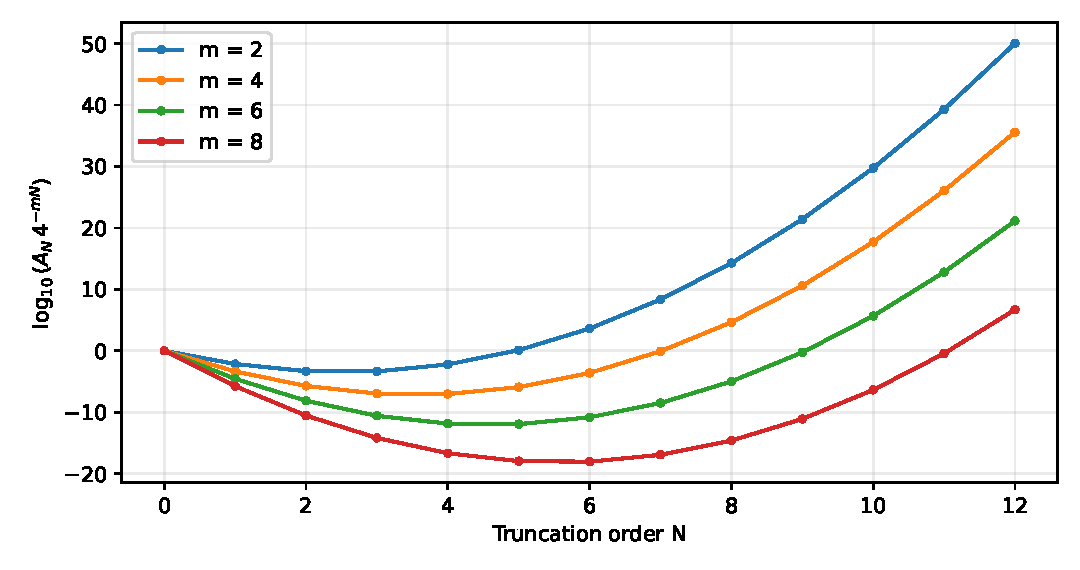
\includegraphics[width=0.93\linewidth]{figures/dc_remainder_bounds.pdf}
 \caption{The proved first-omitted-term bounds $A_N4^{-mN}$.
 Each curve first decreases and then increases. These are values of
 explicit bounds, not measured numerical errors.}
 \label{dc:fig:remainder}
\end{figure}
% ---- DC lines 1225--1315 ----
\chapter{Gaussian localization of the centered zero strings}
\label{dc:sec:complex-center}
The alternating inequality also controls complex translated
arguments, although the complex remainder no longer has a sign.
This is the quantitative refinement asserted in
\cref{dc:thm:overview}.

\begin{proposition}[Complex centered remainder]
\label{dc:prop:complex-center}
Let $h=2^{-m}$, $s=\sigma+\ii\tau$, and $N\ge0$. Then
\begin{align}
 F_{m,1/2}(s)
 &=C(s)\sum_{r=0}^{N-1}(-1)^rc_r
         2^{2rs+2r^2+r}h^{2r}+R_{m,N}(s),
 \label{dc:eq:center-complex-expansion}\\
 \abs{R_{m,N}(s)}
 &\le c_Nh^{2N}C(\sigma+2N)
 =c_Nh^{2N}2^{2N\sigma+2N^2+N}C(\sigma).
 \label{dc:eq:center-complex-bound}
\end{align}
For $s$ in any fixed compact set, an integer $N=N(m)=m/2+O(1)$
can be chosen so that
\begin{equation}
 \sup_s\abs{R_{m,N(m)}(s)}
 \le \exp[-Lm^2/2+O(m)].
 \label{dc:eq:complex-gaussian-error}
\end{equation}
\end{proposition}
\begin{proof}
Use the Taylor remainder of $\Psi(t)=\E e^{-t^2W}$ for real $t\ge0$:
its absolute value after $N$ even terms is at most $c_Nt^{2N}$.
Insert it into \cref{dc:eq:F-exact}; taking absolute values replaces
$u^{s-1}$ by $u^{\sigma-1}$. This proves the first inequality.
The Mellin shift identity proves the equality.

On a compact set let $\sigma\le b$, and bound $C(\sigma)$ by a
constant. Using $c_N\le BR^{-N}$, the logarithm of the bound is at
most
\[
 2LN^2+\{L(1+2b-2m)-\log R\}N+O(1).
\]
Its minimizing integer is $m/2+O(1)$; substitution gives
\cref{dc:eq:complex-gaussian-error}.
\end{proof}

\begin{theorem}[Centered Gaussian zero clusters]
\label{dc:thm:zero-gaussian}
If $s_0$ is a zero of $C$ of multiplicity $d$, then the $d$ zeros of
$D(\cdot,1/2)$ in the cluster approaching $s_0-m$ satisfy
\begin{equation}
 \abs{s-(s_0-m)}
 \le\exp[-Lm^2/(2d)+O_{s_0}(m)].
 \label{dc:eq:center-zero-bound}
\end{equation}
The same conclusion holds for the corresponding off-axis zeros of
$D(\cdot,1)$.
\end{theorem}
\begin{proof}
Choose a small fixed disk $\mathcal K$ about $s_0$ as in
\cref{dc:thm:zero-strings}. Use the truncation $N(m)$ of
\cref{dc:prop:complex-center}. We must check that the finite
multiplier
\[
 S_m(s)=\sum_{r=0}^{N(m)-1}(-1)^rc_r
        2^{2rs+2r^2+r}h^{2r}
\]
remains nonzero near $s_0$ even though its number of terms grows.
For $1\le r<N(m)$, the bound on the logarithm of the $r$th term is
\[
 2Lr^2+\{L(1+2b-2m)-\log R\}r+\log B.
\]
This convex quadratic decreases until a point $m/2+O(1)$.
On the integer interval from $1$ to $N(m)-1$ its maximum is at an
endpoint. The first endpoint is $-2Lm+O(1)$, while the last is
$-Lm^2/2+O(m)$. Thus
$\sup_{s\in\mathcal K}\abs{S_m(s)-1}=O(m2^{-2m})\to0$.
In particular $\abs{S_m}\ge1/2$ for large $m$.

The local lower bound $\abs{C(s)}\ge g_0\abs{s-s_0}^d$ and
\cref{dc:eq:complex-gaussian-error} now allow Rouch\'e on a circle of
radius $\exp[-Lm^2/(2d)+B_1m]$, for a sufficiently large fixed
$B_1$. The comparison term strictly dominates the remainder.
This gives the asserted $d$ zeros. Identity \cref{dc:eq:half-one}
transfers the statement to $a=1$, since these disks are eventually
disjoint from the imaginary axis.
\end{proof}

The proof is deliberately insensitive to the multiplicity of the
limiting zero. For a simple zero the coefficient $1/d$ is absent;
for a multiple zero it is the natural loss produced by a local
factor $(s-s_0)^d$.
% ---- DC lines 1317--1430 ----
\chapter{A non-lognormal measure with exact lognormal moments}
\label{dc:sec:moments}

\section{Moment equality and genuine distinctness}
Let $V$ be lognormal with
\begin{equation}
 \log V\sim N(L/2,L).
 \label{dc:eq:lognormal}
\end{equation}
Its moments are
$\E V^s=\exp[Ls(s+1)/2]$ for real $s$, and indeed for complex $s$.
By \cref{dc:eq:T-moments},
\begin{equation}
 \E T^n=\E V^n\qquad(n\in\Z).
 \label{dc:eq:integer-twins}
\end{equation}
In logarithmic coordinates, the two densities are
\begin{align}
 f_{\log T}(v)
 &=\frac1{C_0}e^{-v^2/(2L)+v/2}H(v),
 \label{dc:eq:T-log-density}\\
 f_{\log V}(v)
 &=\frac1{\sqrt{2\pi L}}e^{-(v-L/2)^2/(2L)}.
 \label{dc:eq:V-log-density}
\end{align}
Their density ratio is
\begin{equation}
 \frac{\dd\mathbb P_T}{\dd\mathbb P_V}(e^v)
 =\frac{\sqrt{2\pi L}\,e^{L/8}}{C_0}H(v).
 \label{dc:eq:density-ratio}
\end{equation}
It is bounded above and below by positive constants, but it is not
constant. Thus the measures are distinct, despite matching every
positive and negative integer moment.

This is an explicit realization of a classical indeterminate moment
problem. The new role of this particular representing measure is
that it is built from the Thue--Morse product and supplies the
scaling limit for the Dirichlet zero problem. The abstract fact that
lognormal moments do not determine a measure is not new
\cite[Section 9]{agk}.

\section{Size bias and the periodic degree of freedom}
The size-biased law of a positive random variable $T$ with finite
mean is defined by
\[
 \E f(T^*)=\frac{\E[Tf(T)]}{\E T}
\]
for bounded measurable $f$. In the present normalization, $\E T=2$.
A change of variables and \cref{dc:eq:K-dilation} give
\begin{equation}
 T^*\overset{d}=2T.
 \label{dc:eq:size-bias}
\end{equation}
Indeed, the density of $T^*$ is $K(t)/(2C_0)$, and the density of
$2T$ is $K(t/2)/(C_0t)=K(t)/(2C_0)$.

More generally, let $p$ be a bounded $L$-periodic measurable function.
The same Mellin substitution used for \cref{dc:eq:C-step} shows that
\begin{equation}
 \int_0^\infty t^n p(\log t)\mu(\dd t)
 =2^{n(n+1)/2}\int_0^\infty p(\log t)\mu(\dd t)
 \quad(n\in\Z).
 \label{dc:eq:periodic-perturb}
\end{equation}
If $p$ has mean zero under $\mu$, then
$(1+\theta p(\log t))\mu(\dd t)$ is a probability measure with the
same integer moments whenever $\abs\theta\,\|p\|_\infty\le1$.
Choosing a nonconstant $p$ produces infinitely many such measures.

To prove \cref{dc:eq:periodic-perturb} for all integer $n$, define
$C_p(s)=\int t^{s-1}K(t)p(\log t)\dd t$. Boundedness of $p$
permits every integral, and its periodicity gives
$C_p(s+1)=2^{s+1}C_p(s)$ by the same substitution. Iteration at
integer arguments proves the formula, including negative indices.

\section{An exact mixture over geometric lattices}
Write every $t>0$ uniquely as $t=v2^k$ with $1\le v<2$ and
$k\in\Z$. Define
\begin{equation}
 \vartheta(v)=\sum_{k\in\Z}v^{-k}2^{-k(k-1)/2}.
 \label{dc:eq:Theta}
\end{equation}
The series converges uniformly for $1\le v\le2$. Then
\begin{equation}
 \mu=\int_1^2 \nu_v\,
        \frac{K(v)\vartheta(v)}{C_0}\frac{\dd v}{v},
 \label{dc:eq:lattice-mixture}
\end{equation}
where the discrete probability measure $\nu_v$ is supported on
$\{v2^k:k\in\Z\}$ and has weights
\begin{equation}
 \nu_v(\{v2^k\})=
 \frac{v^{-k}2^{-k(k-1)/2}}{\vartheta(v)}.
 \label{dc:eq:lattice-weights}
\end{equation}
To verify the identity, split the integral defining $\mu$ into the
intervals $[2^k,2^{k+1})$, substitute $t=2^kv$, and apply
\cref{dc:eq:K-iterate}. This also proves that the mixing density
integrates to one.

Every single $\nu_v$ has the same integer moments:
\begin{equation}
 \int t^n\nu_v(\dd t)=2^{n(n+1)/2}
 \qquad(n\in\Z).
 \label{dc:eq:lattice-moments}
\end{equation}
In fact, shift the summation index by $n$ in the numerator obtained
from \cref{dc:eq:lattice-weights}; completing the exponent gives the
factor $v^{-n}2^{n(n+1)/2}$, which cancels the external $v^n$.
These geometric-lattice moment representatives are classical
Chihara--Leipnik-type laws; see \cite{agk}. Formula
\cref{dc:eq:lattice-mixture} identifies the particular phase mixture
selected by the Thue--Morse completion.
% ---- hand chunk 27-part2-hankel-head.tex ----

\section{Hankel determinants of the slopes and their growth}
\label{ra:sec:moments}
\Cref{dc:cor:Z-Hankel} proved that the Hankel matrices of the slopes
$Z_m(a)$ are positive definite. The uniform expansion of
\cref{ra:thm:asymptotics} makes their growth explicit.

% ---- RA lines 788--836 ----
\subsection{Strict positivity and quantitative Hankel growth}
The substitution $x=1/t$ in $Z_m$ gives
\begin{equation}\label{ra:eq:Cmoment}
 Z_m(a)=\int_0^\infty x^m w_a(x)\dd x,
 \qquad w_a(x)=x^{-1}e^{-a/x}P(1/x)>0.
\end{equation}
Every integer moment exists. Thus the following positivity concerns the
\emph{derivative data} of $D$, not an unrelated Hankel matrix formed
straight from the signs $\eps_n$.

\begin{proposition}[Strict Hankel positivity]\label{ra:prop:Hankel}
For integers $n,\ell\ge0$,
\begin{equation}\label{ra:eq:Hankelpositive}
 \det[Z_{i+j+\ell}(a)]_{i,j=0}^n>0.
\end{equation}
In particular,
\begin{equation}\label{ra:eq:Turan}
 Z_m(a)Z_{m+2}(a)>Z_{m+1}(a)^2,
 \qquad
 \frac{Z_m(a)Z_{m+2}(a)}{Z_{m+1}(a)^2}\longrightarrow2.
\end{equation}
More generally, for fixed $n$ as $m\to\infty$,
\begin{equation}\label{ra:eq:Hankelasympt}
 \begin{split}
 \det[Z_{m+i+j}(a)]_{i,j=0}^n\sim{}&C_0^{n+1}
 2^{\frac{n+1}{2}m(m-1)+mn(n+1)+\frac{n(n+1)(n-1)}3}\\
 &\times\prod_{0\le i<j\le n}(2^j-2^i).
 \end{split}
\end{equation}
The relative error in \eqref{ra:eq:Hankelasympt} is $O(2^{-m})$ for fixed
$a,n$, and is $O(2^{-2m})$ at $a=1/2$.
\end{proposition}
\begin{proof}
The matrix in \eqref{ra:eq:Hankelpositive} is the Gram matrix of
$1,x,\ldots,x^n$ for the strictly positive measure $x^\ell w_a(x)\dd x$.
A nonzero polynomial cannot vanish almost everywhere for this measure, so
the matrix is positive definite.

For the asymptotic determinant, apply Theorem~\ref{ra:thm:asymptotics} to its
finitely many entries. Factor $C_0 2^{m(m-1)/2}$ from each row,
$2^{mi+i(i-1)/2}$ from row $i$, and
$2^{mj+j(j-1)/2}$ from column $j$.
The remaining matrix is $[2^{ij}+O(2^{-m})]$.
Its limiting determinant is the nonzero Vandermonde product
$\prod_{i<j}(2^j-2^i)$. Summing the row and column exponents gives
\eqref{ra:eq:Hankelasympt}; the centered improvement follows from $\alpha_1(1/2)=0$.
The limiting ratio in \eqref{ra:eq:Turan} follows directly from the leading
terms of the three entries.
\end{proof}
% ---- DC lines 1432--1523 ----
\chapter{Exact moment algebra: determinants and orthogonal polynomials}
\label{dc:sec:orthogonal}
The integer moments in \cref{dc:eq:T-moments} make a small amount of
exact algebra available essentially for free. It provides useful
checks on both the normalization and the relation to the
Stieltjes--Wigert moment problem. The algebraic identities themselves
are standard consequences of geometric moments, not independent
priority claims.

\begin{proposition}[Hankel determinant]
\label{dc:prop:determinant}
For every integer $d\ge1$,
\begin{equation}
 \boxed{\displaystyle
 \det\left[2^{(i+j)(i+j+1)/2}\right]_{i,j=0}^{d-1}
 =2^{d^2(d-1)/2}\prod_{k=1}^{d-1}(2^k-1)^{d-k}.}
 \label{dc:eq:hankel-exact}
\end{equation}
\end{proposition}
\begin{proof}
Factor $2^{i(i+1)/2}$ from row $i$ and
$2^{j(j+1)/2}$ from column $j$. The remaining matrix is
$[(2^i)^j]$, whose determinant is the Vandermonde product
$\prod_{0\le i<j<d}(2^j-2^i)$.
In this product factor $2^i$ from each difference. The powers of $2$
from the rows and columns have total exponent
$d(d-1)(d+1)/3$; the extra exponent is
$d(d-1)(d-2)/6$. Their sum is $d^2(d-1)/2$.
A difference $j-i=k$ occurs $d-k$ times, giving the remaining
product.
\end{proof}

Define the Gaussian binomial coefficient at $q=2$ by
\begin{equation}
 \qbinom nk2=\prod_{j=0}^{k-1}
                 \frac{2^{n-j}-1}{2^{j+1}-1}
 \quad(0\le k\le n).
 \label{dc:eq:qbinom}
\end{equation}
Empty products equal one.

\begin{proposition}[Monic orthogonal polynomials]
\label{dc:prop:orthogonal}
The monic degree-$n$ polynomial orthogonal to $1,t,\ldots,t^{n-1}$
under $\mu$ is
\begin{equation}
 \boxed{\displaystyle
 p_n(t)=\sum_{k=0}^n(-1)^{n-k}2^{n(n-k)}\qbinom nk2\,t^k.}
 \label{dc:eq:orthogonal}
\end{equation}
Its squared norm is
\begin{equation}
 \int p_n(t)^2\mu(\dd t)
 =2^{n(3n+1)/2}\prod_{k=1}^n(2^k-1).
 \label{dc:eq:orthogonal-norm}
\end{equation}
The same polynomials and norms apply to every other representing
measure discussed in \cref{dc:sec:moments}.
\end{proposition}
\begin{proof}
For a polynomial $p(t)=\sum_{k=0}^na_kt^k$,
\[
 \int t^jp(t)\mu(\dd t)
 =2^{j(j+1)/2}\sum_{k=0}^n
        a_k2^{k(k+1)/2}(2^j)^k.
\]
Thus orthogonality for $j=0,\ldots,n-1$ is equivalent to the
polynomial identity
\[
 \sum_{k=0}^na_k2^{k(k+1)/2}z^k
 =2^{n(n+1)/2}\prod_{j=0}^{n-1}(z-2^j).
\]
Expanding the product by the finite $q$-binomial identity gives
\cref{dc:eq:orthogonal}. This proves both orthogonality and monicity.
Strict positivity of the Hankel matrices guarantees uniqueness.
The norm is the ratio of the size-$(n+1)$ and size-$n$ Hankel
determinants; substitution of \cref{dc:eq:hankel-exact} gives
\cref{dc:eq:orthogonal-norm}. Alternatively, the same ratio follows
by triangular Gram--Schmidt elimination. Every integral used here
is a polynomial moment, so it is unchanged for any representing
measure with those moments.
\end{proof}

For example,
\[
 p_0(t)=1,\qquad p_1(t)=t-2,\qquad
 p_2(t)=t^2-12t+16.
\]
The norm of $p_1$ is $8-4=4$, agreeing with
\cref{dc:eq:orthogonal-norm}. These low-degree checks are sensitive to
the easily confused alternatives $2^{n(n-1)/2}$ and
$2^{n(n+1)/2}$ in the moment normalization.
% ---- DC lines 1525--1586 ----
\chapter{Identical asymptotic series, different positive functions}
\label{dc:sec:flat-twins}
The moment interpretation gives a concrete nonuniqueness result for
the all-orders expansion itself. Let $V$ be the lognormal variable
in \cref{dc:eq:lognormal}, independent of the same $W$, and set
\begin{equation}
 \widetilde{\calH}(x)=\E e^{-xV^2W}.
 \label{dc:eq:Htilde}
\end{equation}

\begin{theorem}[A completely monotone beyond-all-orders ambiguity]
\label{dc:thm:flat-twins}
The functions $\calH$ and $\widetilde{\calH}$ are distinct, completely
monotone functions with identical derivatives of every order at
zero. Both satisfy the same alternating bound
\cref{dc:eq:alternating-bound}. Consequently, for every $N\ge0$,
\begin{equation}
 \abs{\calH(x)-\widetilde{\calH}(x)}\le2A_Nx^N
 \qquad(x\ge0).
 \label{dc:eq:flat-twin-bound}
\end{equation}
Optimizing $N$ as in \cref{dc:cor:optimal} gives a logarithmic-Gaussian
upper bound for their difference at small $x$.
\end{theorem}
\begin{proof}
Equality of the integer moments of $T$ and $V$ gives
\[
 \frac{\E(T^2W)^r}{r!}
 =\frac{\E(V^2W)^r}{r!}=A_r
\]
for every integer $r\ge0$. The proof of
\cref{dc:thm:alternating} applies unchanged to both Laplace transforms,
so the derivatives and remainder bounds agree. Subtracting the
same finite polynomial gives \cref{dc:eq:flat-twin-bound}.

Suppose nevertheless that the two functions were identical.
Uniqueness of Laplace transforms for probability measures on
$[0,\infty)$ would imply $T^2W\overset d=V^2W$.
For every real $r>0$, all moments involved are finite and
$\E W^r>0$, so independence permits cancellation:
\[
 \E T^{2r}\,\E W^r=\E V^{2r}\,\E W^r
 \quad\Longrightarrow\quad Q(2r)=1.
\]
The identity theorem would then force $Q\equiv1$, contradicting
\cref{dc:prop:C-Fourier}. Thus the functions are distinct.
\end{proof}

The factor $2$ in \cref{dc:eq:flat-twin-bound} is convenient rather than
optimal: since both functions lie in the same interval between
successive alternating truncations, one can in fact replace it by
$1$. Keeping the weaker bound makes clear that even the triangle
inequality already proves flatness. Either version is enough to
show that every coefficient of the asymptotic expansion can be
known exactly while the function still is not uniquely specified.

This phenomenon is not an arbitrary addition of a small oscillatory
term. Both realizations are positive Laplace transforms and satisfy
all complete-monotonicity inequalities. Thus positivity, smoothness,
and a full asymptotic series still leave a nontrivial ambiguity.
The Thue--Morse product supplies the extra information selecting
$\calH$ rather than its lognormal replacement.
% ---- RA lines 876--1001 ----
\chapter{Classification of completely monotone dyadic solutions}\label{ra:sec:classification}

\section{The measure theorem}
We use the Bernstein representation theorem: a completely monotone
function on $(0,\infty)$ is the Laplace transform of a unique positive
Radon measure on $[0,\infty)$, with finite Laplace transform at every
positive argument. One reference stating both representation and uniqueness
is Aguech--Jedidi~\cite[Theorem~1]{aguech-jedidi}.

\begin{theorem}[All positive dyadic solutions]\label{ra:thm:classification}
A function $f:(0,\infty)\to\R$ is completely monotone and satisfies
\begin{equation}\label{ra:eq:dyadicequation}
 f(a)=f(a/2)-f((a+1)/2)
\end{equation}
if and only if there is a positive Radon measure $\nu$ on $(0,\infty)$
with $\nu(2B)=\nu(B)$ such that
\begin{equation}\label{ra:eq:frepresent}
 f(a)=\int_0^\infty e^{-at}P(t)\,\nu(\dd t).
\end{equation}
The measure is unique. It is determined by an arbitrary finite positive
measure $\nu_0$ on the half-open fundamental interval $[1,2)$, and the
correspondence is explicitly
\begin{equation}\label{ra:eq:shellrepresentation}
 f(a)=\int_{[1,2)}\sum_{j\in\Z}
          e^{-a2^jv}P(2^jv)\,\nu_0(\dd v).
\end{equation}
The zero measure corresponds to the zero solution.
\end{theorem}
\begin{proof}
Suppose first that $f$ is completely monotone. Write
$f(a)=\int_{[0,\infty)}e^{-at}\,\mu(\dd t)$ by Bernstein's theorem.
For a measure $\mu$, denote by $\mu(2\,\dd u)$ the pushforward under
$t\mapsto t/2$, so it assigns mass $\mu(2B)$ to a Borel set $B$.
Equation \eqref{ra:eq:dyadicequation} and uniqueness of Laplace transforms give
\begin{equation}\label{ra:eq:mumeasure}
 \mu(\dd u)=(1-e^{-u})\mu(2\,\dd u).
\end{equation}
This also proves $\mu(\{0\})=0$.
Since $P(u)>0$ for $u>0$, define
$\nu(\dd u)=P(u)^{-1}\mu(\dd u)$. It is locally finite on $(0,\infty)$.
Using $P(u)=(1-e^{-u})P(2u)$ in \eqref{ra:eq:mumeasure} yields
$\nu(\dd u)=\nu(2\,\dd u)$, exactly the stated invariance.
Uniqueness follows from uniqueness of $\mu$.

Conversely, let $\nu$ be positive and invariant. Its mass on $[1,2)$ is
finite by local finiteness. Partitioning $(0,\infty)$ into the disjoint
half-open intervals $[2^j,2^{j+1})$ gives \eqref{ra:eq:shellrepresentation}.
At $j\to-\infty$, the bound \eqref{tm:eq:flat-bound} with arbitrarily large $N$
makes the shell sum converge, even after multiplication by any fixed
power of $t$. At $j\to+\infty$, the factor $e^{-at}$ dominates every
power. The convergence is locally uniform for $a>0$ and persists under
all $a$-derivatives. Thus \eqref{ra:eq:frepresent} is finite and completely
monotone. The scaling equation of $P$ and invariance of $\nu$ verify
\eqref{ra:eq:dyadicequation} directly. Finally, a finite measure on $[1,2)$
extends uniquely by scaling to such a measure on $(0,\infty)$.
\end{proof}

This classification includes discrete, absolutely continuous, and singular
measures. It does not secretly assume that a density with respect to
$\dd t/t$ exists.

\section{Normalization fixes mass, not phase}
\begin{corollary}[The normalized solution simplex]\label{ra:cor:normalization}
For the solution in Theorem~\ref{ra:thm:classification},
\begin{equation}\label{ra:eq:normalization}
 f(1/2)=\nu_0([1,2)).
\end{equation}
Consequently, the normalized solutions $f(1/2)=L$ are exactly the
mixtures of
\begin{equation}\label{ra:eq:phasefunctions}
 f_\theta(a)=L\sum_{j\in\Z}
      e^{-a2^{j+\theta}}P(2^{j+\theta}),\qquad 0\le\theta<1.
\end{equation}
Distinct phases give distinct functions. Their uniform phase average is
canonical:
\begin{equation}\label{ra:eq:canonicalaverage}
 Z_0(a)=\int_0^1 f_\theta(a)\dd\theta.
\end{equation}
\end{corollary}
\begin{proof}
The identity
\begin{equation}\label{ra:eq:telescoper}
 e^{-t/2}P(t)=P(t)-P(t/2)
\end{equation}
gives, for every fixed $v>0$,
\[
 \sum_{j\in\Z}e^{-2^{j-1}v}P(2^jv)
 =\lim_{J\to\infty}\{P(2^Jv)-P(2^{-J-1}v)\}=1.
\]
Insert this into \eqref{ra:eq:shellrepresentation} and use positivity to
interchange sum and integral. This proves \eqref{ra:eq:normalization}.
The extremal measures with mass $L$ are point masses
$L\delta_{2^\theta}$; the representation is affine and injective,
so their functions are the extremal normalized solutions.
Distinct phases have disjoint multiplicative lattices, and uniqueness of
Laplace transforms distinguishes the functions.
For the last identity, substitute $t=2^{j+\theta}$ on each shell, so
$\dd t/t=L\dd\theta$.
\end{proof}

In particular,
\begin{equation}\label{ra:eq:canonicalnorms}
 Z_0(1/2)=L,\qquad Z_0(1)=L/2,
 \qquad\Gamma_0^{\mathrm{TM}}(1/2)=2.
\end{equation}
Every normalized solution also has $f(1)=L/2$, because the equation
at $a=1$ reads $f(1)=f(1/2)-f(1)$.
Thus evaluating only at either of these two points conceals the
nonuniqueness. The computations below use $a=1/3$ instead.

\section{Nonuniqueness persists for entire differential towers}
Given an invariant positive measure $\nu$, define, for $\rho\in\R$,
\begin{equation}\label{ra:eq:generalizedC}
 Z_\rho^\nu(a)=\int_0^\infty t^{-\rho}e^{-at}P(t)\,\nu(\dd t).
\end{equation}
The endpoint argument in the classification proof shows that these
integrals are finite and completely monotone for every fixed $\rho$.
For integer levels,
\begin{equation}\label{ra:eq:nutowerlaws}
 (Z_m^\nu)'=-Z_{m-1}^\nu\quad(m\ge1),\qquad
 Z_m^\nu(a)=2^m\{Z_m^\nu(a/2)-Z_m^\nu((a+1)/2)\}.
\end{equation}
Thus the phase freedom is compatible with every level of the differential
ladder and every dyadic equation. Moreover, $Z_m^\nu(a)\to0$ as
$a\to\infty$, by dominated convergence with any fixed positive lower
bound on $a$. Vanishing at infinity does not eliminate this freedom.
% ---- RA lines 1003--1114 ----
\chapter{Universal coefficients and beyond-all-orders ambiguity}\label{ra:sec:ambiguity}

\section{The same coefficient calculus works for every phase measure}
For a nonzero invariant positive measure $\nu$, set
\begin{equation}\label{ra:eq:Knu}
 C_\nu(s)=\int_0^\infty t^s\W(t)\,\nu(\dd t),\qquad
 \Theta_\nu(\rho)=2^{-\rho(\rho-1)/2}C_\nu(-\rho).
\end{equation}
The Gaussian envelope on each shell proves that $C_\nu$ is entire and
positive on the real axis. Invariance and \eqref{dc:eq:K-dilation} imply
\begin{equation}\label{ra:eq:Knurecurrence}
 C_\nu(s+1)=2^{s+1}C_\nu(s).
\end{equation}
Consequently $\Theta_\nu$ is one-periodic and positive on the real axis.

\begin{theorem}[Universal high-order coefficients]\label{ra:thm:universal}
For every nonzero invariant positive measure $\nu$, the expansion
\begin{equation}\label{ra:eq:universalexp}
 \frac{Z_\rho^\nu(a)}{2^{\rho(\rho-1)/2}\Theta_\nu(\rho)}
 =\sum_{k=0}^{N-1}\alpha_k(a)2^{-k\rho}+\mathcal R_N^\nu(\rho,a)
\end{equation}
has exactly the same coefficient polynomials as in
Theorem~\ref{ra:thm:asymptotics}, and
\begin{equation}\label{ra:eq:universalremainder}
 |\mathcal R_N^\nu(\rho,a)|
 \le M_{I,r}r^{-N}2^{N(N+1)/2-N\rho}.
\end{equation}
In particular, the relative remainder bound is independent of $\nu$.
\end{theorem}
\begin{proof}
Write $\rho=m+\theta$ as before. Scaling by $2^{-m}$ in the invariant
measure and using \eqref{ra:eq:Qfinitelevel} gives
\[
 Z_{m+\theta}^\nu(a)
 =2^{m(m-1)/2+m\theta}
   \int_0^\infty t^{-\theta}\W(t)B_a(2^{-m}t)\,\nu(\dd t).
\]
Apply the global Taylor estimate and replace the $K$-recurrence in the
proof of Theorem~\ref{ra:thm:asymptotics} by
\eqref{ra:eq:Knurecurrence}. Positivity permits the same absolute remainder
estimate. The moment ratios are identical, so no coefficient changes.
\end{proof}

\section{Normalized towers can agree to every formal order}
\begin{theorem}[Beyond-all-orders nonuniqueness]\label{ra:thm:ambiguity}
There are infinitely many invariant positive measures $\nu\ne\dd t/t$
for which
\begin{equation}\label{ra:eq:ambiguitynormalizations}
 Z_0^\nu(1/2)=L,\qquad C_\nu(0)=C_0.
\end{equation}
For each of them and every fixed $a>0$, the two sequences
$Z_m^\nu(a)$ and $Z_m(a)$ have the same complete formal expansion in
powers of $2^{-m}$, with the same leading constant.
More quantitatively, they may be constructed so that, for every compact
$I\subset(0,\infty)$, $0<r<4\pi$, and integer $N\ge1$,
\begin{equation}\label{ra:eq:ambiguitybound}
 \frac{|Z_m^\nu(a)-Z_m(a)|}{C_0\,2^{m(m-1)/2}}
 \le |\eta|M_{I,r}r^{-N}2^{N(N+1)/2-Nm},\qquad a\in I,
\end{equation}
where $0<|\eta|<1$ is a freely chosen perturbation parameter.
The corresponding functions $a\mapsto Z_0^\nu(a)$ are nevertheless distinct.
\end{theorem}
\begin{proof}
Choose a nonzero real trigonometric polynomial $p$ of period one satisfying
\begin{equation}\label{ra:eq:twopconditions}
 \int_0^1p(y)\dd y=0,\qquad
 \int_0^\infty\W(t)p(\log_2t)\frac{\dd t}{t}=0,
 \qquad \|p\|_\infty\le1.
\end{equation}
Such choices exist in an infinite-dimensional family. To see this
concretely, take any finite-dimensional span of nonconstant sines and
cosines. Every element already has zero ordinary mean; the weighted
condition imposes at most one linear equation. With two or more
independent modes there is a nonzero solution, which can be rescaled.
Increasing the number of modes gives arbitrarily large families.

Define
\begin{equation}\label{ra:eq:nupperturb}
 \nu(\dd t)=\{1+\eta p(\log_2t)\}\frac{\dd t}{t},
 \qquad0<|\eta|<1.
\end{equation}
This is positive and dyadically invariant. The first zero mean gives
$\nu([1,2))=L$; the second gives $C_\nu(0)=C_0$.
The periodic-perturbation identity \eqref{dc:eq:periodic-perturb} gives equality of all integer Mellin moments.
Theorem~\ref{ra:thm:universal}, at integer orders, therefore gives the same
formal expansion and leading constant.

For the stronger bound, use the exact renormalization of the difference:
\[
 Z_m^\nu(a)-Z_m(a)
 =\eta\,2^{m(m-1)/2}\int_0^\infty
       \W(t)p(\log_2t)B_a(2^{-m}t)\frac{\dd t}{t}.
\]
Every term of the Taylor polynomial integrates to zero by
\eqref{dc:eq:periodic-perturb}. The global Taylor remainder, $|p|\le1$, and
$C(N)=2^{N(N+1)/2}C_0$ give \eqref{ra:eq:ambiguitybound}.
Finally, the Laplace measures $P(t)\nu(\dd t)$ are different because
$p$ is nonzero and $P>0$. Laplace uniqueness implies that the functions
$Z_0^\nu$ are different.
\end{proof}

Choosing $N$ as in \eqref{ra:eq:tau}--\eqref{ra:eq:optimal}, with $\rho=m$,
makes the relative difference in \eqref{ra:eq:ambiguitybound} at most
\begin{equation}\label{ra:eq:ambiguityoptimal}
 |\eta|2^{1/8}M_{I,r}\,
       2^{-\frac12(m+\log_2r-1/2)^2}.
\end{equation}
This gives a concrete mathematical meaning to ``invisible to all formal
high-order corrections.'' It does not say that two distinct towers have
the same exact values. Nor does it rule out characterization by a different
asymptotic variable: the next section uses $a\downarrow0$ precisely to
recover the missing information.
% ---- RA lines 1116--1241 ----
\chapter{A boundary characterization of the canonical tower}\label{ra:sec:uniqueness}

\section{A single slope limit selects the invariant measure}
\begin{theorem}[Boundary uniqueness]\label{ra:thm:uniqueness}
Let $f$ be completely monotone on $(0,\infty)$ and satisfy
\eqref{ra:eq:dyadicequation}. Then
\begin{equation}\label{ra:eq:slopecondition}
 \lim_{a\downarrow0}(-a f'(a))=1
\end{equation}
holds if and only if
\begin{equation}\label{ra:eq:canonicalunique}
 f(a)=Z_0(a)=\int_0^\infty e^{-at}P(t)\frac{\dd t}{t}.
\end{equation}
No separate point normalization is needed.
More generally, replacing the limit one by a nonnegative constant $c$
selects $f=cC_0$.
\end{theorem}
\begin{proof}
Let $\nu$ be the invariant representing measure from
Theorem~\ref{ra:thm:classification}. Fix $s>0$ and set $a_N=s2^{-N}$.
Scaling by $2^N$ in the measure gives
\begin{equation}\label{ra:eq:slopescale}
 -a_N f'(a_N)
 =\int_0^\infty st e^{-st}P(2^Nt)\,\nu(\dd t).
\end{equation}
For each fixed $t>0$, $P(2^Nt)\to1$.
The dominating kernel $st e^{-st}$ is integrable against $\nu$:
on shells tending to zero it is $O_s(2^j)$, and on shells tending to
infinity it has exponential decay. Each shell has the same finite mass.
Dominated convergence therefore yields
\begin{equation}\label{ra:eq:slopelimit}
 \lim_{N\to\infty}(-a_N f'(a_N))
   =s\int_0^\infty t e^{-st}\,\nu(\dd t).
\end{equation}
If \eqref{ra:eq:slopecondition} holds, the right side equals one for every
$s>0$. Hence the measure $t\nu(\dd t)$ has Laplace transform $1/s$.
This is the Laplace transform of Lebesgue measure $\dd t$ on
$(0,\infty)$, and uniqueness gives $t\nu(\dd t)=\dd t$.
Thus $\nu(\dd t)=\dd t/t$, proving necessity.

For the canonical measure, substitution $u=at$ gives
\[
 -aC_0'(a)=a\int_0^\infty e^{-at}P(t)\dd t
       =\int_0^\infty e^{-u}P(u/a)\dd u\longrightarrow1
\]
by $0<P\le1$ and dominated convergence.
The proof with limit $c$ identifies $t\nu(\dd t)=c\dd t$ in exactly the
same way, including $c=0$.
\end{proof}

Equation \eqref{ra:eq:slopelimit} explains the obstruction in the other
solutions: in general, the dyadic boundary limits retain the phase
information of $\nu$. A full limit as $a\downarrow0$, rather than a
limit along one selected dyadic sequence, removes that information.
The hypothesis genuinely means a limit through \emph{all} positive $a$.

\section{A finite-part condition is sufficient}
\begin{corollary}[Finite-part characterization]\label{ra:cor:finitepart}
Within the completely monotone solutions of \eqref{ra:eq:dyadicequation},
the existence of a finite limit
\begin{equation}\label{ra:eq:finitepartcondition}
 \lim_{a\downarrow0}\{f(a)+\log a\}\in\R
\end{equation}
is equivalent to $f=Z_0$. For the canonical function, the limit is
\begin{equation}\label{ra:eq:kappa}
 \kappa=-\gamma+
     \int_0^1\frac{P(t)}t\dd t+
     \int_1^\infty\frac{P(t)-1}t\dd t,
\end{equation}
where $\gamma$ is Euler's constant.
\end{corollary}
\begin{proof}
Complete monotonicity implies convexity. For $0<h<1$, the two secant
bounds around $a$ give
\begin{equation}\label{ra:eq:convexbounds}
 \frac{f(a)-f((1+h)a)}h
 \le -af'(a)
 \le\frac{f((1-h)a)-f(a)}h.
\end{equation}
Under \eqref{ra:eq:finitepartcondition}, the left and right expressions tend,
as $a\downarrow0$, to $\log(1+h)/h$ and $-\log(1-h)/h$ respectively.
Letting $h\downarrow0$ proves \eqref{ra:eq:slopecondition}, and
Theorem~\ref{ra:thm:uniqueness} applies.

For the converse, split the canonical integral as
\[
 Z_0(a)=\int_0^1e^{-at}\frac{P(t)}t\dd t
       +\int_1^\infty e^{-at}\frac{P(t)-1}t\dd t
       +\int_1^\infty e^{-at}\frac{\dd t}{t}.
\]
The first two integrals converge to their values at $a=0$ by
Lemma~\ref{tm:lem:P-bounds}. The last is the exponential integral
$E_1(a)=-\log a-\gamma+o(1)$, which gives \eqref{ra:eq:kappa}.
\end{proof}

The finite-part hypothesis is stronger than the slope hypothesis as a
condition on arbitrary functions, but both select exactly the same member
of the dyadic completely monotone family.

\section{Uniqueness of the full differential hierarchy}
\begin{corollary}[Canonical gamma-tower characterization]\label{ra:cor:towerunique}
Suppose $f_0,f_1,\ldots$ are completely monotone functions on
$(0,\infty)$ satisfying
\begin{equation}\label{ra:eq:toweraxioms}
 \begin{aligned}
 f_m(a)&=2^m\{f_m(a/2)-f_m((a+1)/2)\} &&(m\ge0),\\
 f_m'(a)&=-f_{m-1}(a) &&(m\ge1),
 \end{aligned}
\end{equation}
and $-af_0'(a)\to1$ as $a\downarrow0$.
Then $f_m=Z_m$ for every $m\ge0$. Equivalently, the functions
$\exp((-1)^m m!f_m)$ are exactly the hierarchy in
\eqref{ra:eq:Gammadef}.
\end{corollary}
\begin{proof}
Theorem~\ref{ra:thm:uniqueness} gives $f_0=Z_0$.
Inductively, if $f_{m-1}=Z_{m-1}$, the differential ladder says that
$f_m-Z_m$ is a constant $d_m$.
Subtracting the two level-$m$ dyadic equations gives
$d_m=2^m(d_m-d_m)=0$. This completes the induction.
\end{proof}

This supplies a normalization and a proof of uniqueness in a precise
positive class. It does not establish every possible Weierstrass-product
or complex-analytic assertion one might include in a broader Barnes-type
program. The two issues should be kept separate.
% ---- DC lines 1588--1691 ----
\chapter{Extension to sparse digit sequences in other integer bases}
\label{dc:sec:bases}
The completion is not restricted to base two. This section records
the extension with enough detail to identify exactly where
integrality of the base is used.

For a real number $b>1$, define
\begin{equation}
 P_b(t)=\prod_{j\ge0}(1-e^{-b^jt}),\qquad
 X_b=\sum_{j\ge1}b^{-j}U_j,\qquad
 \Phi_b(t)=\E e^{-tX_b},\qquad K_b=P_b\Phi_b.
 \label{dc:eq:base-products}
\end{equation}
Now $X_b$ is supported on $[0,1/(b-1)]$ and has mean
$a_b=1/[2(b-1)]$. The same cancellation gives
\begin{equation}
 K_b(bt)=\frac{K_b(t)}t,
 \qquad C_b(s+1)=b^{s+1}C_b(s),
 \label{dc:eq:base-mellin}
\end{equation}
where $C_b(s)=\int_0^\infty t^{s-1}K_b(t)\dd t$.
Thus the normalized measure has moments $b^{n(n+1)/2}$ for every
integer $n$, and the exact logarithmic profile is periodic with
period $\log b$.

When $b\ge2$ is an integer, define $\mathcal S_b$ to be the
nonnegative integers whose base-$b$ digits are all zero or one.
For $n\in\mathcal S_b$, let $w_b(n)$ be the number of nonzero
digits. The product expansion gives
\begin{equation}
 P_b(t)=\sum_{n\in\mathcal S_b}(-1)^{w_b(n)}e^{-nt},
 \label{dc:eq:base-digit-series}
\end{equation}
and hence the sparse signed Dirichlet series
\begin{equation}
 D_b(s,a)=\sum_{n\in\mathcal S_b}
       \frac{(-1)^{w_b(n)}}{(n+a)^s}.
 \label{dc:eq:base-Dirichlet}
\end{equation}
Absolute convergence holds at least in $\Rea s>\log_b2$:
the integers in $\mathcal S_b$ below $b^k$ are exactly $2^k$ in
number, and comparison by base-$b$ blocks proves convergence there.
The Mellin integral continues the series to an entire function just
as before.

\begin{theorem}[Integer-base zero strings]
\label{dc:thm:base-zeros}
For every integer $b\ge2$ and every $a>0$, $D_b(\cdot,a)$ has
infinitely many nonreal zeros in the left half-plane. More precisely,
if $s_0$ is a zero of $C_b$ of multiplicity $d$, the corresponding
clusters approach $s_0-m$ with error smaller than $b^{-Am}$ for
every fixed $A>0$.
At the centered shift $a=a_b$, their error is bounded by
\begin{equation}
 \exp\left[-\frac{\log b}{2d}m^2+O(m)\right].
 \label{dc:eq:base-zero-rate}
\end{equation}
\end{theorem}
\begin{proof}
All the completion and Mellin estimates replace $L$ by $\log b$.
The nonconstancy proof is still valid: because $b^j$ is an integer,
$P_b(x+2\pi\ii)=P_b(x)\to0$, whereas a constant-profile elementary
Gaussian expression would have a nonzero limit there.
The normalized periodic Mellin function is therefore nonconstant,
entire, positive on the real axis, and of order at most two.
Lemma \ref{dc:lem:periodic-zero} supplies a nonreal zero.

Put $B_{b,a}(t)=e^{-at}/\Phi_b(t)$. Since $X_b$ has positive
probability in every neighborhood of zero, the proof of the global
Taylor remainder in \cref{dc:lem:B-global} applies. With $h=b^{-m}$,
exact rescaling gives
\[
 b^{-m(m-1)/2+ms}\Gamma(s-m)D_b(s-m,a)
 =\int_0^\infty u^{s-1}K_b(u)B_{b,a}(hu)\dd u.
\]
At poles of the Gamma factor, the left side is interpreted through
its entire Mellin numerator. The $j$th coefficient is again a multiple of $C_b(s+j)$, and
\cref{dc:eq:base-mellin} factors out $C_b(s)$. The proof of
\cref{dc:thm:zero-strings} now applies verbatim.

For the centered bound,
\[
 B_{b,a_b}(z)=\prod_{j\ge1}
       \frac{z/(2b^j)}{\sinh(z/(2b^j))}
\]
is the Laplace transform in $z^2$ of
\[
 W_b=\sum_{j,n\ge1}\frac{E_{j,n}}{4\pi^2b^{2j}n^2}.
\]
Its first moment-generating pole is at $R_b=4\pi^2b^2$.
Removing the first pole as in \cref{dc:thm:c-asymptotic} bounds its
coefficients by a constant times $R_b^{-r}$. The counterpart of
\cref{dc:eq:center-complex-bound} then has exponent
$2(\log b)N^2-2m(\log b)N+O(N)$.
Optimizing at $N=m/2+O(1)$ and repeating the Rouch\'e argument
proves \cref{dc:eq:base-zero-rate}.
\end{proof}

For noninteger real $b>1$, the positive product, Mellin identity,
and moment construction still hold. The boundary-periodicity step
used to prove nonconstancy does not automatically survive, and
\cref{dc:eq:base-digit-series} is no longer an ordinary integer-indexed
Dirichlet series. We do not silently extend the integer-base zero
claim to that setting.
% ---- DC lines 1693--1797 ----
\chapter{An explicit Fourier formula for the logarithmic profile}
\label{dc:sec:log-Fourier}
The proofs above need neither zeta values nor an evaluated constant.
For reproducible computation, however, it is useful to make the
profile explicit. Mellin analysis of harmonic sums is a standard
method \cite{fgd}; the calculation is included here to fix every
sign and normalization.

Let $\gamma$ denote Euler's constant and $\gamma_1$ the first
Stieltjes constant in
\begin{equation}
 \zeta(1+z)=\frac1z+\gamma-\gamma_1z+O(z^2).
 \label{dc:eq:stieltjes-convention}
\end{equation}
Define
\begin{equation}
 \chi_k=\frac{2\pi\ii k}{L},\qquad
 c_*=-\frac L{12}-\frac{\pi^2/12-\gamma^2/2-\gamma_1}{L}.
 \label{dc:eq:cstar}
\end{equation}

\begin{proposition}[Exact profile formula]
\label{dc:prop:logH}
For real $v$,
\begin{equation}
 \boxed{\displaystyle
 \log H(v)=c_*-\frac1L\sum_{k\in\Z\setminus\{0\}}
       \Gamma(\chi_k)\zeta(1+\chi_k)e^{-\chi_kv}.}
 \label{dc:eq:logH-Fourier}
\end{equation}
The Fourier series and every fixed derivative converge absolutely.
\end{proposition}
\begin{proof}
For $\Rea z>0$, expanding $\log(1-e^{-t})$ into exponentials and
integrating termwise gives
\[
 \int_0^\infty t^{z-1}\log(1-e^{-t})\dd t
 =-\Gamma(z)\zeta(z+1).
\]
Summing the dyadic dilates, also absolutely for $\Rea z>0$, gives
\begin{equation}
 \log P(t)=-\frac1{2\pi\ii}
 \int_{c-\ii\infty}^{c+\ii\infty}
 \frac{\Gamma(z)\zeta(z+1)}{1-2^{-z}}t^{-z}\dd z,
 \qquad c>0.
 \label{dc:eq:logP-Mellin}
\end{equation}
This Mellin inversion is justified by exponential decay of the
Gamma factor on vertical lines.

Move the line to $\Rea z=-\delta$, with $0<\delta<1$.
The crossed poles are $z=0$ and $z=\chi_k$, $k\ne0$.
One may use horizontal sides at heights
$2\pi(N+1/2)/L$, which stay away from the zeros of the denominator.
Stirling's estimate for $\Gamma$, polynomial bounds for $\zeta$
on this fixed vertical strip, and the bound on the denominator show
that the horizontal integrals tend to zero. On the new vertical
line the integral is $O(t^\delta)$ as $t\downarrow0$.
The residue sum converges absolutely because
$\abs{\Gamma(\chi_k)}$ decays exponentially in $\abs k$.

At a nonzero $\chi_k$, the derivative of $1-2^{-z}$ is $L$, so
its residue contributes
$-\Gamma(\chi_k)\zeta(1+\chi_k)t^{-\chi_k}/L$.
At zero, use
\begin{align*}
 \Gamma(z)\zeta(1+z)
 &=\frac1{z^2}+\left(\frac{\pi^2}{12}
             -\frac{\gamma^2}{2}-\gamma_1\right)+O(z),\\
 \frac1{1-e^{-Lz}}&=\frac1{Lz}+\frac12+\frac{Lz}{12}+O(z^3).
\end{align*}
Multiplication by $t^{-z}$ gives the contribution
\[
 -\frac{(\log t)^2}{2L}+\frac{\log t}{2}+c_*.
\]
Consequently,
\[
 \log P(t)=-\frac{(\log t)^2}{2L}+\frac{\log t}{2}+c_*
 -\frac1L\sum_{k\ne0}\Gamma(\chi_k)\zeta(1+\chi_k)t^{-\chi_k}
 +O(t^\delta).
\]
Since $\log\Phi(t)=O(t)$, comparison with the definition of $H$
gives the claimed Fourier expression plus $O(t^\delta)$ for small
$t$. Finally replace $t$ by $2^{-m}t$. Both the profile and the
Fourier sum are invariant under this substitution, while the error
tends to zero. This turns the asymptotic identity into the exact
formula \cref{dc:eq:logH-Fourier}. Exponential Gamma decay absorbs any
fixed derivative multiplier $\chi_k^r$.
\end{proof}

\begin{figure}[t]
 \centering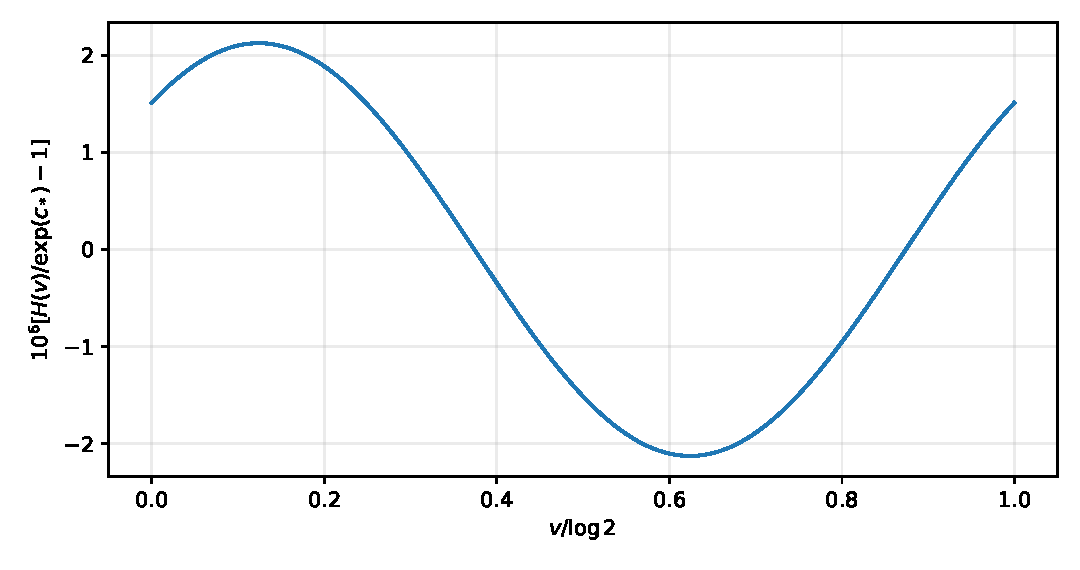
\includegraphics[width=0.93\linewidth]{figures/dc_periodic_profile.pdf}
 \caption{The nonconstant profile $H$ over one logarithmic period.
 The vertical scale is in parts per million relative to $e^{c_*}$.
 This small oscillation is not a negligible detail for the complex
 zero problem.}
 \label{dc:fig:profile}
\end{figure}

The Fourier series for $\log H$ and the Fourier series for $H$
should not be confused. To use \cref{dc:eq:C-Fourier}, first exponentiate
\cref{dc:eq:logH-Fourier}, then calculate the coefficients $h_k$ of the
resulting positive function. Substituting the coefficients of
$\log H$ directly into \cref{dc:eq:C-Fourier} gives an incorrect
normalization and shifts the computed zeros.
% ---- DC lines 1799--1923 ----
\chapter{Numerical experiments and reproducibility}
\label{dc:sec:numerics}

\section{What was computed}
The accompanying script \path{verification/source2/code/verify.py} performs exact rational
coefficient and determinant checks, evaluates $K$ by its products,
evaluates the profile by \cref{dc:eq:logH-Fourier}, and compares direct
Mellin quadrature with the Fourier--Gaussian representation.
It also solves for selected zeros in the normalized variable, using
\cref{dc:eq:F-exact} rather than a very large unnormalized Gamma factor.
The files under \path{verification/source2/data/} contain the numerical outputs.
The completion constant and the displayed limiting zero agree in
separate 60- and 80-digit runs. The script
\path{verification/source2/code/check_original_mellin.py} additionally tests the first
listed Dirichlet zero directly in the original integral
\cref{dc:eq:M-def}, for both $a=1/2$ and $a=1$, without using the
completion to construct its integrand.

These are high-precision floating-point experiments. Their reported
residuals are not interval-arithmetic error certificates. The
existence theorems and the signed remainder bounds are proved
analytically above and do not depend on interpreting a small
floating-point residual as a proof.

The normalizing constant is approximately
\begin{equation}
 C_0=0.7507219804078709592097079140506346947658\ldots.
 \label{dc:eq:C0-numeric}
\end{equation}
One numerically observed simple zero of $C$, chosen in a real
fundamental strip, is
\begin{equation}
 s_0\approx
 0.1240623273169621334141320413937
 +6.7214865334392714744741792585671\,\ii.
 \label{dc:eq:s0-numeric}
\end{equation}
The word ``one'' is intentional: the computation does not establish
that this is the lowest-height nonreal zero, nor that all zeros are
simple. The normalized derivative $Q'(s_0)$ is numerically extremely
close to $2\pi\ii$, consistent with a leading two-term Fourier
balance, but that observation is not used in the proof.

\begin{table}[ht]
\centering\small
\begin{tabular}{@{}rlll@{}}
\toprule
$m$&$\Rea s_m$&$\Ima s_m$&$\abs{s_m-(s_0-m)}$\\
\midrule
4&$-3.8759680374867420$&$6.7214963407429050$&$3.19093\cdot10^{-5}$\\
6&$-5.8759376731062212$&$6.7214865336192914$&$4.59882\cdot10^{-10}$\\
8&$-7.8759376726830382$&$6.7214865334392717$&$4.19307\cdot10^{-16}$\\
\bottomrule
\end{tabular}
\caption{Numerical zeros of $D(s,1/2)$ and, by
\cref{dc:eq:half-one}, of $D(s,1)$. The distances refer to the
higher-precision value of $s_0$ stored in the data file.}
\label{dc:tab:zeros}
\end{table}

The centered slope ratios provide an independent positive-axis
check:
\begin{table}[ht]
\centering
\begin{tabular}{@{}rl@{}}
\toprule
$m$&$Z_m(1/2)/(C_0\,2^{m(m-1)/2})$\\
\midrule
0&$0.9233074275823854568421676411$\\
2&$0.9934028797641805193051831301$\\
4&$0.9995677618356360314893011938$\\
6&$0.9999728805385416834067380219$\\
8&$0.9999983046075012694941809752$\\
\bottomrule
\end{tabular}
\caption{Direct Mellin quadrature of the exact samples
$\calH(4^{-m})$. The script checks the signed inequalities for
truncation orders one through seven.}
\label{dc:tab:ratios}
\end{table}

\section{Stable product evaluation}
For positive $t$, compute $\log P(t)$ as a sum of
$\log(-\operatorname{expm1}(-2^jt))$ rather than by subtracting nearly
equal floating-point numbers. Its omitted large-scale terms decrease
doubly exponentially.

For $\Phi(t)$, first apply enough halvings that the remaining argument
$v$ lies in $(0,1]$. Multiply the finitely many removed factors
exactly at working precision. The infinite remaining tail is then
computed from
\begin{equation}
 \log\Phi(v)=-\frac v2+
 \sum_{r\ge1}\frac{B_{2r}v^{2r}}{2r(2r)!(2^{2r}-1)}.
 \label{dc:eq:Phi-numeric}
\end{equation}
This avoids multiplying hundreds of factors close to one. Both the
product route and the Fourier route are retained in the script so
that they can cross-check one another.

For the zeta values in \cref{dc:eq:logH-Fourier}, the points
$1+2\pi\ii k/L$ are exact dyadic resonances. An implementation using
$\zeta(s)=\eta(s)/(1-2^{1-s})$ naively can lose precision there,
since both numerator and denominator vanish. The supplied code
explicitly requests Euler--Maclaurin evaluation of $\zeta$.
In the tested \texttt{mpmath} environment this avoided a visible
loss of accuracy in the profile. This is an implementation detail,
not a mathematical singularity of $\zeta$ at these points.

\section{Why the Mellin quadrature is manageable}
In logarithmic coordinates, the integrand for $C$ is a Gaussian
multiplied by a bounded periodic function and $e^{sv}$.
For a fixed complex $s$, the center of its absolute Gaussian
majorant is $L(\Rea s+1/2)$. The code chooses its finite integration
interval using that center and the requested precision.
At the centered shift, $0<\Psi(2^{-m}e^v)\le1$, so the same
Gaussian tail estimate also controls $F_{m,1/2}$.

The finite interval and quadrature discretization are not
interval-certified in this implementation. Repeating at increased
precision and comparing two analytic representations gives a strong
consistency check, while the proofs supply the logical foundation.
The exact rational calculations, by contrast, are exact: the
coefficient formulas and Hankel determinants are evaluated with
\texttt{SymPy} rationals and integers.
% ---- hand chunk 28-part2-numerics-ra-head.tex ----

\section{Independent evaluation of the slopes and of the phases}
\label{ra:sec:numerics}
A second program, retained as \path{verification/source3/verify_results.py},
evaluates the slopes $Z_\rho(a)$ from their original integrals, the
amplitude $\Theta$ on one multiplicative period, and the explicit extremal
solutions of \cref{ra:cor:normalization}, independently of the first
program. Below, $\calH_m$ abbreviates the exact sample $\calH(4^{-m})$ of
\cref{dc:thm:alternating}.

% ---- RA lines 1245--1370 ----
\subsection{Independent integral evaluation}
The archive contains \texttt{verify\_results.py} and two JSON reports.
The coefficient identities were checked exactly with rational symbolic
arithmetic through $k=12$. The numerical calculations were performed
with 48 Gauss--Legendre nodes at 60 decimal digits and repeated with
80 nodes at 80 digits. Both the precision and the quadrature size were
increased; agreement is not based solely on changing the displayed number
of digits.

For $C_0$ and $\Theta$, the program evaluates a single multiplicative
period. Combining \eqref{dc:eq:K-profile} with $t=2^{y+j}$ gives
\begin{equation}\label{ra:eq:onecellTheta}
 \Theta(\rho)=L\,2^{1/8}
 \int_0^1 H(Ly)\sum_{j\in\Z}
 2^{-(j+y+\rho-1/2)^2/2}\dd y.
\end{equation}
Periodicity permits reduction of $\rho$ modulo one.
The rapidly convergent Gaussian shell sum makes this inexpensive.

The $Z_\rho$ checks are evaluated separately from their \emph{original}
$P$-integrals, not by inserting the claimed coefficient expansion or the
$B_a$-renormalization. On logarithmic shells the computation uses
\begin{equation}\label{ra:eq:onecellC}
 \begin{split}
 \frac{Z_\rho(a)}{2^{\rho(\rho-1)/2}}
  =L\int_0^1\sum_{j\in\Z}
  \exp\bigl(&-\rho L(y+j)-a2^{y+j}\\
       &+\log P(2^{y+j})-\tfrac L2\rho(\rho-1)\bigr)\dd y.
 \end{split}
\end{equation}
Small factors are evaluated with \texttt{expm1} to avoid cancellation.
The shell values of $P$ use its own product recurrence. This comparison
can detect an incorrect prefactor or a wrong coefficient in the theorem.

The two runs agree far beyond the digits printed below. For example,
the reported $C_0$ values agree in the first 49 decimal places; their
stored difference is less than $4\cdot10^{-51}$.
The calculations are \emph{not interval-certified}: quadrature stability
and exact symbolic checks support the implementation, while the proofs
establish the theorems. The numerical work does not establish a sharp
constant in the remainder bound or historical novelty.

\subsection{Centered derivative data}
Let
\[
 \calH_m=\frac{Z_m(1/2)}{C_0\,2^{m(m-1)/2}},\quad
 P_2=1-\frac{2^{-2m}}9,\quad
 P_4=P_2+\frac{248}{2025}2^{-4m},\quad
 P_6=P_4-\frac{4806656}{2679075}2^{-6m}.
\]
Table~\ref{ra:tab:centered} compares successive approximations. For fixed
truncation order the improvement agrees with the even powers predicted by
symmetry.

\begin{table}[htbp]
\centering\small
\begin{tabular}{rcccc}
\toprule
$m$ & $|\calH_m-1|$ & $|\calH_m-P_2|$ & $|\calH_m-P_4|$ & $|\calH_m-P_6|$\\
\midrule
4  & $4.322382\,10^{-4}$ & $1.789613\,10^{-6}$ & $7.911730\,10^{-8}$ & $2.782223\,10^{-8}$\\
8  & $1.695392\,10^{-6}$ & $2.850821\,10^{-11}$& $6.353778\,10^{-15}$& $2.031475\,10^{-17}$\\
12 & $6.622738\,10^{-9}$ & $4.350974\,10^{-16}$& $3.799206\,10^{-22}$& $4.918108\,10^{-27}$\\
16 & $2.587007\,10^{-11}$& $6.639065\,10^{-21}$& $2.264533\,10^{-29}$& $1.145315\,10^{-36}$\\
\bottomrule
\end{tabular}
\caption{Absolute errors in the normalized centered expansion. The notation
$x\,10^{-j}$ means $x\times10^{-j}$.}
\label{ra:tab:centered}
\end{table}

At $m=4$, the benefit of further terms is already much less spectacular
than at $m=16$. This is consistent with the fact that the expansion is
divergent: adding indefinitely many terms at a fixed order is not justified.
The full data files also include nonsymmetric shifts and noninteger
orders, for example $a=1$ and $\rho=8.25,8.5,12.75$.

\subsection{The tiny Mellin phase and the visible gamma phase}
The observed relative modulation of $\Theta$ is shown in
Table~\ref{ra:tab:theta}. Its small size is consistent with the exact Fourier
smoothing factor in \eqref{ra:eq:Thetafourier}.

\begin{table}[htbp]
\centering
\begin{tabular}{cc}
\toprule
$\theta$ & $\Theta(\theta)/\Theta(0)-1$\\
\midrule
$1/4$ & $1.289029564918397699\times10^{-18}$\\
$1/2$ & $1.296624062281340296\times10^{-18}$\\
$3/4$ & $7.594497362942597195\times10^{-21}$\\
\bottomrule
\end{tabular}
\caption{Numerical phase variation. Nonconstancy is numerical evidence
here, not an additional theorem assumed elsewhere.}
\label{ra:tab:theta}
\end{table}

For comparison, Table~\ref{ra:tab:phases} gives the explicit extremal
solutions of \eqref{ra:eq:phasefunctions}. Their differences are much easier
to see, although all have $f_\theta(1/2)=L$ and
$f_\theta(1)=L/2$.

\begin{table}[htbp]
\centering
\begin{tabular}{ccc}
\toprule
$\theta$ & $f_\theta(1/3)$ & $-a f_\theta'(a)$ at $a=2^{-24}$\\
\midrule
$0$   & $0.956669839913615728$ & $1.00000628193280958$\\
$1/4$ & $0.956669741884495862$ & $0.99999235648832259$\\
$1/2$ & $0.956665362383835818$ & $0.99999357544426848$\\
$3/4$ & $0.956665460410626991$ & $1.00000750091845969$\\
\bottomrule
\end{tabular}
\caption{Distinct positive normalized solutions. The canonical value is
$Z_0(1/3)=0.956667601148143600\ldots$. The slope column is a finite-$a$
evaluation, not a claimed exact limiting value.}
\label{ra:tab:phases}
\end{table}

The program also checks the dyadic equation away from these special
normalization points, using $a=1.3$ and $\theta=0.27$.
The residual is below $10^{-70}$ in the 80-digit run.
Agreement at $a=1$ alone would be an inadequate test because that value
is forced by the normalization.
% ---- hand chunk 29-part2-questions-head.tex ----

\chapter{A formalization route and further questions}
\label{dc:sec:route}

% ---- DC lines 1982--2015 ----
\section{A proof-oriented dependency chain}
A formal development can be organized into four layers, without
requiring the numerical Fourier formula for the principal theorem.
First prove positivity and normal convergence of $P$ and $\Phi$,
then their two scaling equations. This yields $K(2t)=K(t)/t$ and
positive upper and lower bounds for its logarithmic profile.

Next establish the Gaussian domination needed for the entire Mellin
transform and its derivatives. The Mellin shift, periodicity of $Q$,
and the boundary contradiction proving nonconstancy can then be
formalized independently of coefficient calculations. The zero-free
finite-order lemma and a version of Rouch\'e with multiplicities
complete the complex-analytic layer.

The asymptotic layer consists of the positive-axis global Taylor
bound for $B_a$ and the exact change of variables in
\cref{dc:eq:F-exact}. Once these are available, the all-orders
factorization is a finite-sum integration lemma, and the
supergeometric zero-cluster theorem is a uniform remainder estimate
followed by Rouch\'e.

Finally, the centered layer adds Euler's $\sinh$ product, the
positive exponential-sum law $W$, and an integral Taylor remainder.
It supplies the signed bounds, the coefficient-pole estimate, and
the Gaussian refinement. The finite Bell-polynomial formula and the
Hankel determinant can be developed in a separate exact algebra
module.

The existing atlas names modules such as
\path{ThueMorseBoundaryFlatness.lean} and
\path{ThueMorseEntireContinuation.lean} for relevant background.
No new Lean file is supplied here, and no theorem in this extension
is claimed to have been machine-checked. The dependency chain is a
technical implementation guide, not a formalization status claim.
% ---- DC lines 2017--2078 ----
\section{Further questions suggested by the proved results}
\label{dc:sec:questions}
The following questions concern refinements not needed for any
preceding theorem.

\begin{question}[Zeros in a fundamental strip]
Can the nonreal zeros of $Q$ in $0\le\Rea s<1$ be counted and
localized effectively as their imaginary parts grow? Are they all
simple?
\end{question}
The Fourier--Gaussian representation is a natural starting point.
At increasing height, different Fourier harmonics compete. A
rigorous two-term dominance argument on suitable contours could
produce explicit zero enclosures, but the present computation is
not a proof of such a global pattern.

\begin{question}[Leading exponentially small displacement]
For a simple zero $s_0$ of $C$, determine an asymptotic equivalent,
not just an upper bound, for $s_m-(s_0-m)$ at the centered shift.
\end{question}
All algebraic powers of $2^{-m}$ vanish from the displacement.
The nearest poles of $\Psi$ and the logarithmic-Gaussian saddle
suggest a more detailed exponentially small analysis. Such an
analysis must retain the phase information in $H$; replacing the
completion by its lognormal twin would erase the zeros of the
limiting periodic factor.

\begin{question}[Growing-height zero windows]
How far may $\abs{\Ima s}$ grow with $m$ while the translated
asymptotic expansion remains useful for zero localization?
\end{question}
The remainder bound in \cref{dc:eq:F-remainder-explicit} depends on
$\Rea s$ but not directly on $\Ima s$. The difficulty is instead a
lower bound for $C(s)$ on the contours used by Rouch\'e. Thus this
question couples growth of the periodic entire factor to the
geometry of its zeros.

\begin{question}[Noninteger dilation]
For every real $b>1$, is the logarithmic profile of $K_b$ nonconstant?
What replaces the integer-frequency boundary argument when $b$ is
not an integer?
\end{question}
An affirmative answer would extend the Mellin zero mechanism to a
continuous family of generalized exponential sums. The exact
completion and moment identities already hold; the missing step in
the proof given here is the nonconstancy argument in that greater
generality.

\subsection*{Closing perspective}
The most useful organizing fact is a cancellation between an
expanding product and a contracting one. The Thue--Morse product
alone carries a complicated dyadic scale dependence; the
uniform-convolution transform removes its nonmonomial factor.
The resulting exact law $K(2t)=K(t)/t$ simultaneously explains
lognormal integer moments, the negative-argument scale of the
Dirichlet continuation, the universal factor in every asymptotic
coefficient, and the occurrence of nonreal zero strings.
At the half-shift, symmetry supplies an additional positive
Laplace representation and converts the expansion into certified
inequalities. The log-periodic information is small on the real
axis, but it is precisely the information that survives beyond all
orders and controls the complex zeros.
% ---- hand chunk 2A-part2-ra-outlook-head.tex ----

\section{Further directions for the uniform remainder and the classification}
The classification theorem gives a lesson complementary to the zero
strings. The dyadic functional equation controls how a measure moves between
scales but does not prescribe the distribution of mass within a scale;
one-point normalization determines only that scale's total mass, and even a
full formal expansion at integer orders can fail to recover the missing
phase information. The boundary slope recovers the whole Laplace transform
of the invariant measure and is therefore strong enough to characterize it.
The Fourier formula of \cref{dc:prop:logH} supplies the closed expression for
the amplitude that the uniqueness analysis leaves implicit; the leading
exponentially small discrepancy in \cref{ra:thm:ambiguity}, rather than only
its Gaussian-in-order upper bound, remains to be determined, and the poles
of $B_a$ at imaginary multiples of $4\pi$ together with the chosen phase
measure should enter such a refinement.

% ---- RA lines 1413--1428 ----
A separate quantitative task is to replace the tube supremum $M_{I,r}$ by
simple computable constants optimized for a given shift interval.
The proof of Lemma~\ref{ra:lem:tubebound} already separates a compact region
from a controlled tail, so interval arithmetic could turn it into a
numerical certificate. The present tables should not be mistaken for that
certificate.

The positive-measure classification and the proof of the uniform remainder
also have clear formalization targets: product convergence, pushforward
identities, the Mellin recurrence, Cauchy estimates on a tube, and Laplace
uniqueness. None of these targets requires asserting that the results
already appear in the repository's Lean code. Finally, analogous product
pairs for other dilation factors may produce related invariant-measure
classifications; a radix change must be made at the level of the product
equation rather than by replacing every two in the final formulas without
checking the underlying sequence.
% ---- hand chunk 30-part3-head.tex ----

\part{Rational resonances and coalescing roots}
\label{part:resonances}

\chapter{Scope and the main results}
\label{rr:sec:scope}
The finite Thue--Morse polynomial $P_m(w)=\prod_{j<m}(1-w^{2^j})$ contains
more information than its values at roots of unity. This part investigates
its complete local profile in a window of width $2^{-m}$ around each rational
frequency. The atlas already treats the binary product, Prouhet
cancellation, ordinary power moments, root-of-unity filters, rarefied sums,
and the finite-product bridge to the Fabius--Rvachev system; those are
starting points here. The closest external comparisons are Sobolewski's
root-of-unity recurrence theory for automatic-sequence polynomials
\cite{sobolewski} and Duke--Nguyen's asymptotic theory of infinite
cyclotomic products \cite{duke}; neither recurrence at a rational frequency
nor the use of cyclotomic products is itself new. The intended extensions
are the explicit moving-window factorization, its full derivative calculus,
and the coalescing-root limits. Baake and Coons study higher correlations
\cite{baake-coons}, Gohlke, Kesseb\"ohmer and Schindler generalized spectral
measures \cite{gohlke}, and Cloitre iterated transforms \cite{cloitre};
these concern neighboring problems.


% ---- RR lines 94--122 ----
\section{A guide to the contributions}
There are four main groups of results.

\paragraph{Exact local profiles.}
For a nontrivial odd-order root \(\zeta\), define
\[
 \Qp_{m,\zeta}(z)=\frac{P_m(\zeta\e^{z/2^m})}{P_m(\zeta)}.
\]
Theorem~\ref{rr:thm:profile} gives entire functions \(\Hp_{\zeta,s}\), periodic in the depth phase \(s\), with the exact identity
\[
 \Qp_{m,\zeta}(z)\Hp_{\zeta,0}(z/2^m)=\Hp_{\zeta,s}(z).
\]
Theorem~\ref{rr:thm:correction} turns this into a convergent, all-orders expansion with an explicit remainder bound. Theorem~\ref{rr:thm:moments} differentiates it into a closed formula for every twisted power moment.

\paragraph{Coalescing-root universality.}
At a primitive dyadic root of order \(2^r\), a polynomial of depth \(m=r+M\) has a zero of multiplicity \(M\). Removing that zero gives a normalized function \(\Np_{r,M}\). For a fixed root, its limit is \(\Up\), the Fabius transform. Theorem~\ref{rr:thm:hierarchy} determines the different limits when \(r\) grows with \(M\). In particular,
\[
 r4^{-M}\longrightarrow\lambda
 \quad\Longrightarrow\quad
 \e^{-r2^{-M}z/(2\pi\ii)}\Np_{r,M}(z)
 \longrightarrow \Up(z)\e^{\lambda z^2/(8\pi^2)}.
\]
This Gaussian--Fabius limit is the most distinctive new derivation in the part.

\paragraph{Cyclotomic aggregation.}
Theorem~\ref{rr:thm:norm} multiplies the rational-frequency profiles into an integer dilation quotient of \(\Up\). Theorem~\ref{rr:thm:regularity} classifies the associated probability laws: odd dilation factors give singular continuous laws; even factors give densities of an explicitly determined, finite differentiability class.

\paragraph{Geometry and exact arithmetic.}
Theorem~\ref{rr:thm:zeros} determines the entire zero divisor of each profile. Theorem~\ref{rr:thm:depth} gives eventual recurrences for weighted residue sums, with completely explicit characteristic roots. These results supply independent checks on the analytic constructions.
% ---- hand chunk 31-part3-conventions.tex ----

\chapter{The finite product and the Fabius transform}
\label{rr:sec:background}
\section{The positive comparison function}
This part works with the Fabius transform in the moment-generating
normalization
\begin{equation}\label{rr:eq:Umgf}
 \Up(z)=\E e^{zX}=\Phi(-z),
\end{equation}
where $X=\sum_{k\ge1}2^{-k}V_k$ is the uniform sum \eqref{tm:eq:X} (the
letters $V_k$ are used for the uniform variables here) and $\Phi$ is the
transform of \eqref{tm:eq:Phi}. Define the removable entire function
$g(z)=(e^z-1)/z=\psi(-z)$, $g(0)=1$, and its finite and infinite dyadic
products
\begin{equation}\label{rr:eq:U}
 \Up_M(z)=\prod_{k=1}^Mg(z/2^k),\qquad
 \Up(z)=\prod_{k=1}^{\infty}g(z/2^k).
\end{equation}
By \cref{tm:lem:Phi}, $\Up$ is entire, its zeros are the points $4\pi\ii n$,
$n\ne0$, with multiplicity $1+v_2(n)$, and it obeys the denominator-free
identities
\begin{equation}\label{rr:eq:Utail}
 \Up_M(z)\Up(z/2^M)=\Up(z),\qquad
 \Up(2z)=g(z)\Up(z).
\end{equation}
We use the bounded Fabius normalization $F(x)=\Prob(X\le x)$ of
\eqref{tm:eq:Fabius-cdf}, which agrees on $[0,1]$ with the classical Fabius
construction \cite{fabius}; $X$ has a smooth compactly supported density.
The centered product is
\begin{equation}\label{rr:eq:Usinh}
 \Up(z)=e^{z/2}\prod_{k\ge1}\frac{\sinh(z/2^{k+1})}{z/2^{k+1}},
\end{equation}
by \eqref{tm:eq:M} with $Y=2X-1$. Thus the familiar sinc product is already
present, but the rational profiles below will not individually be
transforms of positive measures.

% ---- RR lines 209--221 ----
\section{An explicit coefficient convention}
Let \(b_n\) denote Bernoulli numbers with \(b_1=-1/2\), and define
\begin{equation}
 \beta_1=\frac12,\qquad \beta_n=\frac{b_n}{n}\quad(n\geq2).
 \label{rr:eq:beta}
\end{equation}
Then
\begin{equation}
 \log g(z)=\sum_{n\geq1}\beta_n\frac{z^n}{n!},\qquad
 \log\Up(z)=\sum_{n\geq1}\frac{\beta_n}{2^n-1}\frac{z^n}{n!}.
 \label{rr:eq:Ulog}
\end{equation}
The first equality follows by differentiating the logarithm and using the generating function of the Bernoulli numbers; summing the dyadic geometric series gives the second. These logarithms are the branches that vanish at zero. The second series has radius \(4\pi\), the distance to the first zero of \(\Up\).
% ---- RR lines 240--387 ----
\chapter{Odd-order rational resonance profiles}
\label{rr:sec:profiles}

\section{Backward phases}
Fix an odd integer \(q\geq3\), an integer \(a\) with \(1\leq a<q\), and
\begin{equation}
 \zeta=\e^{2\pi\ii a/q},\qquad L=\ord_q(2).
\end{equation}
The root need not be primitive. Negative exponents of \(2\) in exponents of \(\zeta\) always mean inverses modulo \(q\). Equivalently, reduce the exponent of \(2\) modulo \(L\). Define
\begin{equation}
 a_{s,k}=\zeta^{2^{s-k}},\qquad
 \Hp_{\zeta,s}(z)=\prod_{k\geq1}
 \frac{1-a_{s,k}\e^{z/2^k}}{1-a_{s,k}},
 \qquad s\in\Z/L\Z.
 \label{rr:eq:H}
\end{equation}
Every denominator is nonzero. The index \(k\) follows the binary orbit backwards because the last, largest-scale factor of \(P_m\) becomes the first factor after rescaling.

\begin{theorem}[Exact profile factorization]
\label{rr:thm:profile}
The products \(\Hp_{\zeta,s}\) are entire and satisfy \(\Hp_{\zeta,s}(0)=1\). If \(m\geq0\) and \(s\equiv m\pmod L\), then
\begin{equation}
 \boxed{\quad
 \frac{P_m(\zeta\e^{z/2^m})}{P_m(\zeta)}
 \Hp_{\zeta,0}(z/2^m)=\Hp_{\zeta,s}(z).
 \quad}
 \label{rr:eq:exactH}
\end{equation}
In particular, along \(m\equiv s\pmod L\),
\begin{equation}
 \Qp_{m,\zeta}(z)\longrightarrow\Hp_{\zeta,s}(z)
 \label{rr:eq:Hlimit}
\end{equation}
uniformly on every compact subset of \(\C\), together with all derivatives.
\end{theorem}
\begin{proof}
Put \(d=\min_{0\leq j<L}|1-\zeta^{2^j}|>0\). For \(|z|\leq R\), the \(k\)-th factor differs from one by at most
\begin{equation}
 \frac{R\e^{R/2^k}}{d2^k}\leq\frac{R\e^{R/2}}{d2^k}.
 \label{rr:eq:factorbound}
\end{equation}
The sum converges. The standard product criterion, which follows directly from the Cauchy criterion and \(\prod(1+u_k)\leq\exp(\sum u_k)\) for \(u_k\geq0\), gives compact-uniform convergence and entireness.

Reindex the finite product by \(k=m-j\). Its normalized factors are exactly the first \(m\) factors of \(\Hp_{\zeta,s}\). For the omitted factors write \(k=m+\ell\). Then
\[
 a_{s,m+\ell}=\zeta^{2^{-\ell}},\qquad
 z/2^{m+\ell}=(z/2^m)/2^\ell.
\]
Their product is \(\Hp_{\zeta,0}(z/2^m)\), proving \eqref{rr:eq:exactH}. This tail tends to one uniformly on compact sets and is nonzero there for all sufficiently large \(m\). The limit follows, and Cauchy's integral formula on slightly larger compact sets gives convergence of every derivative.
\end{proof}

The denominator-free form \eqref{rr:eq:exactH} is important. A quotient formula without that qualification would appear to have poles at zeros of the tail even though the finite polynomial profile is entire.

\section{Closed cumulants}
For \(n\geq1\) and \(w\neq1\), define the rational function
\begin{equation}
 \Li_{1-n}(w)=\left(w\frac{\mathrm d}{\mathrm dw}\right)^{n-1}
                  \frac{w}{1-w}.
 \label{rr:eq:Lirational}
\end{equation}
This is the rational continuation of the usual nonpositive-order polylogarithm; no infinite series at a root of unity is intended. For example,
\[
 \Li_0(w)=\frac{w}{1-w},\quad
 \Li_{-1}(w)=\frac{w}{(1-w)^2},\quad
 \Li_{-2}(w)=\frac{w(1+w)}{(1-w)^3}.
\]

\begin{theorem}[Finite formulas for all cumulants]
\label{rr:thm:cumulants}
Write, near zero,
\begin{equation}
 \log\Hp_{\zeta,s}(z)=\sum_{n\geq1}\kappa_{\zeta,s,n}\frac{z^n}{n!}.
\end{equation}
Then
\begin{equation}
 \boxed{\quad
 \kappa_{\zeta,s,n}=
 -\frac{\displaystyle\sum_{k=1}^L2^{-kn}
       \Li_{1-n}(\zeta^{2^{s-k}})}{1-2^{-Ln}}.
 \quad}
 \label{rr:eq:kappa}
\end{equation}
In particular, all cumulants and Taylor coefficients belong to \(\Q(\zeta)\).
\end{theorem}
\begin{proof}
Repeated differentiation gives
\[
 \left.\frac{\mathrm d^n}{\mathrm dz^n}\log(1-w\e^z)\right|_{z=0}
 =-\Li_{1-n}(w).
\]
The compact convergence estimates used above justify summing derivatives in a zero-free neighborhood of the origin. Thus the cumulant is
\(-\sum_{k\geq1}2^{-kn}\Li_{1-n}(a_{s,k})\).
The phase is periodic with period \(L\); summing each residue class of \(k\) yields \eqref{rr:eq:kappa}. Every summand is a rational function of \(\zeta\).
\end{proof}

Define two coefficient families explicitly by
\begin{align}
 h_{\zeta,s,j}
 &=\frac1{j!}\B_j(\kappa_{\zeta,s,1},\ldots,\kappa_{\zeta,s,j}),
 \label{rr:eq:hcoeff}\\
 c_{\zeta,j}
 &=\frac1{j!}\B_j(-\kappa_{\zeta,0,1},\ldots,-\kappa_{\zeta,0,j}).
 \label{rr:eq:ccoeff}
\end{align}
Then \(\Hp_{\zeta,s}(z)=\sum h_{\zeta,s,j}z^j\) and
\(1/\Hp_{\zeta,0}(z)=\sum c_{\zeta,j}z^j\) near zero. In particular,
\begin{align}
 c_0&=1,&c_1&=-\kappa_1,\\
 c_2&=\tfrac12(\kappa_1^2-\kappa_2),&
 c_3&=\tfrac16(-\kappa_1^3+3\kappa_1\kappa_2-\kappa_3),
 \label{rr:eq:firstc}
\end{align}
where the suppressed cumulants have phase zero.

\section{All orders with a certified analytic bound}
\begin{theorem}[Convergent depth expansion]
\label{rr:thm:correction}
For \(s\equiv m\pmod L\) and every fixed \(N\geq0\),
\begin{equation}
 \Qp_{m,\zeta}(z)
 =\Hp_{\zeta,s}(z)\sum_{j=0}^N c_{\zeta,j}z^j2^{-mj}
       +O_{R,N,\zeta}(2^{-(N+1)m}),\qquad |z|\leq R.
 \label{rr:eq:allorders}
\end{equation}
More explicitly, put
\[
 d=\min_j|1-\zeta^{2^j}|,\quad \rho=d/4,\quad
 M_R=\exp(R\e^{R/2}/d),\quad
 J_\rho=\exp(2\rho\e^{\rho/2}/d).
\]
Whenever \(R2^{-m}<\rho\), the absolute remainder in \eqref{rr:eq:allorders} is at most
\begin{equation}
 M_RJ_\rho\,
 \frac{(R2^{-m}/\rho)^{N+1}}{1-R2^{-m}/\rho}.
 \label{rr:eq:certified}
\end{equation}
The infinite expansion converges whenever \(|z|2^{-m}\) is smaller than the distance from zero to the nearest zero of \(\Hp_{\zeta,0}\).
\end{theorem}
\begin{proof}
Equation~\eqref{rr:eq:factorbound} bounds \(|\Hp_{\zeta,s}(z)|\) by \(M_R\). On \(|w|\leq\rho\), write each factor of \(\Hp_{\zeta,0}\) as \(1+v_k\). The estimates give
\[
 \sum|v_k|\leq\rho\e^{\rho/2}/d,
 \qquad |v_k|\leq\rho\e^{\rho/2}/(2d)<1/2,
\]
since \(d\leq2\). The inequality \((1-u)^{-1}\leq\e^{2u}\) for \(0\leq u\leq1/2\) bounds the reciprocal product by \(J_\rho\). Cauchy's coefficient estimate therefore gives \(|c_j|\leq J_\rho\rho^{-j}\). Summing the geometric tail and multiplying by \(M_R\) proves \eqref{rr:eq:certified}. The exact factorization proves convergence throughout the zero-free Taylor disc of the reciprocal.
\end{proof}

This is stronger than a merely formal asymptotic series. The error correction is the Taylor expansion of one fixed analytic reciprocal, evaluated at the shrinking argument \(z2^{-m}\).
% ---- RR lines 389--507 ----
\chapter{Zeros, symmetry, and refinement of the profiles}
\label{rr:sec:geometry}

\section{The complete zero divisor}
A normal product is especially informative when all its factors have explicit zeros. Write \(\zeta=\e^{2\pi\ii a/q}\), with \(q\) odd and \(1\leq a<q\), as before. We use \(v_2(t)=v_2(|t|)\) for nonzero integers, and take the phase \(s\) modulo \(L\).

\begin{theorem}[Zeros and their exact multiplicities]
\label{rr:thm:zeros}
The zeros of \(\Hp_{\zeta,s}\) are precisely
\begin{equation}
 z=\frac{2\pi\ii t}{q},\qquad
 t\in2\Z\setminus\{0\},\qquad
 t\equiv-a2^s\pmod q.
 \label{rr:eq:Hzeros}
\end{equation}
The multiplicity of this zero is \(v_2(t)\). Equivalently, the zeros are
\begin{equation}
 z=\frac{4\pi\ii\ell}{q},\qquad
 \ell\equiv-a2^{s-1}\pmod q,
 \quad\text{with multiplicity }1+v_2(\ell).
 \label{rr:eq:Hzerosell}
\end{equation}
Here negative powers of two in congruences mean inverses modulo \(q\).
\end{theorem}
\begin{proof}
Choose an integer \(v_k\) representing \(a2^{s-k}\pmod q\). The \(k\)-th factor vanishes exactly when
\[
 z=\frac{2\pi\ii}{q}\,2^k(qj-v_k),\qquad j\in\Z.
\]
Consequently, at a point \(z=2\pi\ii t/q\), this factor vanishes if and only if \(2^k\mid t\) and \(t\equiv-a2^s\pmod q\). Each such zero of the factor is simple. For a fixed nonzero \(t\), precisely \(k=1,\ldots,v_2(t)\) contribute. The congruence excludes \(t=0\), since \(a\not\equiv0\pmod q\).

It remains to rule out zeros introduced by the infinite tail. On every compact set the sum of the distances of the factors from \(1\) converges. A sufficiently late tail consists of nonzero factors close to \(1\), so its logarithm converges normally and its product never vanishes. Thus the zeros and multiplicities are exactly those already counted.
\end{proof}

\begin{corollary}[The exact radius of a reciprocal expansion]
Let \(b\in\{1,\ldots,q-1\}\) represent \(-a2^{s-1}\pmod q\). The Taylor series of \(1/\Hp_{\zeta,s}(z)\) at zero has radius
\begin{equation}
 \frac{4\pi}{q}\min\{b,q-b\}.
 \label{rr:eq:reciprocalradius}
\end{equation}
\end{corollary}
\begin{proof}
The closest integers to zero in the progression \(b+q\Z\) are \(b\) and \(b-q\). The reciprocal has a pole at each zero of \(\Hp_{\zeta,s}\), so the nearest one determines the radius.
\end{proof}

\begin{corollary}[Non-holonomicity]
No \(\Hp_{\zeta,s}\) satisfies a nontrivial homogeneous linear differential equation with polynomial coefficients.
\end{corollary}
\begin{proof}
For arbitrarily large \(k\), choose an odd integer \(u\) in the residue class \(-a2^{s-k}\pmod q\); odd representatives exist because \(q\) is odd. Then \(t=2^ku\) gives a zero of multiplicity \(k\). In particular the multiplicities are unbounded, at infinitely many distinct points.

Suppose a nonzero entire function satisfies a homogeneous differential equation of order \(r\), with nonzero leading polynomial. At a point where that polynomial does not vanish, a zero of multiplicity at least \(r\) sets all \(r\) initial data to zero. Local uniqueness for the corresponding first-order system forces the function to vanish identically. Only finitely many exceptional points are zeros of the leading polynomial, contradicting the unbounded multiplicities just established. An order-zero equation is impossible for a nonzero entire function as well.
\end{proof}

This conclusion is only non-holonomicity, often called non-D-finiteness. It does not establish differential transcendence with respect to nonlinear differential equations.

\section{A real centered Fourier profile}
\begin{proposition}[Reflection and strict concavity]
For every phase,
\begin{equation}
 \Hp_{\zeta,s}(z)=\e^z\overline{\Hp_{\zeta,s}(-\overline z)}.
 \label{rr:eq:reflection}
\end{equation}
Hence \(\operatorname{Re}\kappa_{\zeta,s,1}=1/2\), every even cumulant is real, and every odd cumulant of order at least three is purely imaginary.

The function
\begin{equation}
 G_{\zeta,s}(t)=\e^{-\ii t/2}\Hp_{\zeta,s}(\ii t)
 \label{rr:eq:centeredG}
\end{equation}
is real on the real axis. Between any two consecutive distinct real zeros, \(\log|G_{\zeta,s}(t)|\) is strictly concave, and \(|G_{\zeta,s}|\) has exactly one critical point, a strict maximum.
\end{proposition}
\begin{proof}
For \(|a|=1\), \(a\ne1\), direct algebra gives
\[
 \frac{1-a\e^u}{1-a}
 =\e^u\overline{\frac{1-a\e^{-\overline u}}{1-a}}.
\]
Multiplying over the profile factors and using \(\sum_{k\geq1}2^{-k}=1\) gives \eqref{rr:eq:reflection}. Comparing Taylor coefficients of the logarithms near zero proves the cumulant assertions.

Write \(a_{s,k}=\e^{\ii\theta_k}\), where \(\theta_k\) is chosen periodically. The elementary sine identity gives
\begin{equation}
 G_{\zeta,s}(t)=\prod_{k\geq1}
 \frac{\sin(\theta_k/2+t/2^{k+1})}{\sin(\theta_k/2)}.
 \label{rr:eq:sineprofile}
\end{equation}
All factors are real for real \(t\). On compact subintervals avoiding the zeros, the logarithmic derivatives converge normally. Indeed, in the tail the sine denominators remain uniformly bounded away from zero, while each differentiation supplies a factor \(2^{-k-1}\). Thus
\begin{equation}
 \frac{\dd^2}{\dd t^2}\log|G_{\zeta,s}(t)|
 =-\sum_{k\geq1}4^{-k-1}
 \csc^2(\theta_k/2+t/2^{k+1})<0.
 \label{rr:eq:concavity}
\end{equation}
If consecutive distinct zeros are \(\alpha<\beta\), the logarithmic derivative tends to \(+\infty\) as \(t\downarrow\alpha\), and to \(-\infty\) as \(t\uparrow\beta\), with the corresponding zero multiplicities as positive coefficients. By strict monotonicity it crosses zero exactly once. Since \(G\) does not vanish inside the interval, this proves the assertion about its absolute value.
\end{proof}

\section{A cyclic refinement equation}
Set
\begin{equation}
 A_\zeta=\prod_{j=0}^{L-1}(1-\zeta^{2^j}),\qquad b=2^L.
 \label{rr:eq:Acycle}
\end{equation}
The value of this product is unchanged by a cyclic shift of the exponents.

\begin{proposition}[One step and one complete cycle]
The profiles satisfy
\begin{align}
 \Hp_{\zeta,s}(2z)
 &=\frac{1-\zeta^{2^{s-1}}\e^z}{1-\zeta^{2^{s-1}}}
     \Hp_{\zeta,s-1}(z),\label{rr:eq:onestep}\\
 \Hp_{\zeta,s}(bz)
 &=\frac{P_L(\zeta^{2^s}\e^z)}{A_\zeta}\Hp_{\zeta,s}(z).
 \label{rr:eq:cycle}
\end{align}
\end{proposition}
\begin{proof}
In the first formula, split off the first factor and shift \(k\) to \(k-1\) in the tail. For the second, split off the first \(L\) factors and put \(j=L-k\). Periodicity gives \(\zeta^{2^{s-L+j}}=\zeta^{2^{s+j}}\), identifying the numerator with the finite Thue--Morse product. The remaining product is the original phase.
\end{proof}
The coefficients of this refinement equation are generally complex. The existence of such an equation does not by itself make an individual profile the transform of a positive measure.
% ---- RR lines 509--674 ----
\chapter{Exact twisted moments and arithmetic progressions}
\label{rr:sec:moments}

\section{All moments from a finite Bell polynomial}
For \(h\geq0\), define
\begin{equation}
 T_{m,h}(\zeta)=\sum_{n<2^m}\eps_n\zeta^n n^h.
 \label{rr:eq:Tmoment}
\end{equation}
The coefficients \(h_{\zeta,s,j}\) and \(c_{\zeta,j}\) were defined in \eqref{rr:eq:hcoeff} and \eqref{rr:eq:ccoeff}.

\begin{theorem}[Closed twisted-moment formulas]
\label{rr:thm:moments}
For every \(m,h\geq0\), with \(s\equiv m\pmod L\),
\begin{align}
 \frac{T_{m,h}(\zeta)}{P_m(\zeta)}
 &=h!\sum_{j=0}^h h_{\zeta,s,j}c_{\zeta,h-j}2^{mj}
 \label{rr:eq:momentcoeff}\\
 &=\B_h\bigl(2^m\kappa_{\zeta,s,1}-\kappa_{\zeta,0,1},
      \ldots,2^{mh}\kappa_{\zeta,s,h}-\kappa_{\zeta,0,h}\bigr).
 \label{rr:eq:momentBell}
\end{align}
All sums defining the cumulants and Bell polynomials are finite. Thus these formulas require no auxiliary recurrence in \(m\) or \(h\).
\end{theorem}
\begin{proof}
The exponential generating function of the left side is
\[
 \sum_{h\geq0}\frac{T_{m,h}(\zeta)}{P_m(\zeta)}\frac{t^h}{h!}
 =\frac{P_m(\zeta\e^t)}{P_m(\zeta)}
 =\frac{\Hp_{\zeta,s}(2^mt)}{\Hp_{\zeta,0}(t)}
\]
in a neighborhood of zero, by Theorem~\ref{rr:thm:profile}. Multiplying the two Taylor series gives \eqref{rr:eq:momentcoeff}. Taking a logarithm first, then applying the defining generating function of the complete Bell polynomials, gives \eqref{rr:eq:momentBell}.
\end{proof}

In particular,
\begin{align}
 \frac{T_{m,1}}{P_m}&=2^m\kappa_{s,1}-\kappa_{0,1},\\
 \frac{T_{m,2}}{P_m}&=(2^m\kappa_{s,1}-\kappa_{0,1})^2
                         +2^{2m}\kappa_{s,2}-\kappa_{0,2}.
\end{align}
The two parts of the result have different uses. Formula~\eqref{rr:eq:momentBell} is compact and suitable for symbolic evaluation. Formula~\eqref{rr:eq:momentcoeff} exhibits the exact finite collection of depth scales \(2^{mj}\).

\section{The first nontrivial example: order three}
Let \(\omega=\e^{2\pi\ii/3}\). Then \(L=2\), \(A_\omega=3\), and
\begin{equation}
 P_{2t}(\omega)=3^t,\qquad P_{2t+1}(\omega)=3^t(1-\omega).
 \label{rr:eq:omegaP}
\end{equation}
Substitution into the finite cumulant formula gives
\begin{align}
 \kappa_{\omega,0,1}&=\frac12+\frac{\ii\sqrt3}{18},&
 \kappa_{\omega,1,1}&=\frac12-\frac{\ii\sqrt3}{18},\\
 \kappa_{\omega,s,2}&=\frac19,&
 \kappa_{\omega,s,4}&=-\frac1{45},\\
 \kappa_{\omega,0,3}&=-\frac{\ii\sqrt3}{81},&
 \kappa_{\omega,1,3}&=\frac{\ii\sqrt3}{81}.
 \label{rr:eq:omegakappa}
\end{align}
For example, \(\Li_0(\omega)=-1/2+\ii\sqrt3/6\), and the order-one weighted sum is
\[
 -\frac{\frac12\Li_0(\omega^2)+\frac14\Li_0(\omega)}{1-1/4}
 =\frac12+\frac{\ii\sqrt3}{18}.
\]
The first centered moment consequently has the exact form
\begin{equation}
 \frac{T_{m,1}(\omega)}{P_m(\omega)}-\frac{2^m-1}{2}
 =\frac{\ii\sqrt3}{18}\bigl((-1)^m2^m-1\bigr).
 \label{rr:eq:omegacenter}
\end{equation}
The imaginary term is not an error: the weights \(\eps_n\omega^n\) are complex.

\section{Weighted sums in an arithmetic progression}
For an odd \(q\geq3\), a residue \(b\in\Z\), and \(h\geq0\), put
\begin{equation}
 S^{(q)}_{m,b,h}=\sum_{\substack{0\leq n<2^m\\n\equiv b\pmod q}}
                  \eps_n n^h.
 \label{rr:eq:progression}
\end{equation}
These are integers. Let \(\zeta_q=\e^{2\pi\ii/q}\), \(L=\ord_q2\), and
\[
 A_a=\prod_{j=0}^{L-1}(1-\zeta_q^{a2^j}),\qquad 1\leq a<q.
\]
Use the same \(L\) for all roots, even when one has smaller order.

\begin{theorem}[An explicit eventual recurrence in the block depth]
\label{rr:thm:depth}
Fix \(q,b,h\), and fix \(s\in\{0,\ldots,L-1\}\). Whenever \(Lt+s>h\),
\begin{equation}
 S^{(q)}_{Lt+s,b,h}
 =\sum_{a=1}^{q-1}\sum_{j=0}^h
 C_{a,s,b,h,j}\,(A_a2^{Lj})^t,
 \label{rr:eq:depthsum}
\end{equation}
where, writing the subscripts \(a\) for the root \(\zeta_q^a\),
\begin{equation}
 C_{a,s,b,h,j}=
 \frac{\zeta_q^{-ab}}q\,P_s(\zeta_q^a)\,h!\,
 c_{a,h-j}h_{a,s,j}2^{sj}.
 \label{rr:eq:depthC}
\end{equation}
In particular, the ordinary generating series in \(t\) is rational, with denominator dividing
\begin{equation}
 \prod_{a=1}^{q-1}\prod_{j=0}^{h}(1-A_a2^{Lj}T)\in\Z[T].
 \label{rr:eq:depthdenom}
\end{equation}
Equivalently, the sequence satisfies an eventual integer-coefficient linear recurrence whose characteristic polynomial can be taken to be
\(\prod_{a,j}(X-A_a2^{Lj})\).
\end{theorem}
\begin{proof}
The elementary root-of-unity filter is
\[
 \frac1q\sum_{a=0}^{q-1}\zeta_q^{a(n-b)}
 =\begin{cases}1,&n\equiv b\pmod q,\\0,&\text{otherwise}.
 \end{cases}
\]
After multiplication by \(\eps_nn^h\) and summation, it yields
\[
 S^{(q)}_{m,b,h}=\frac1q\sum_{a=0}^{q-1}\zeta_q^{-ab}T_{m,h}(\zeta_q^a).
\]
For \(m>h\), the term \(a=0\) vanishes by Prouhet cancellation. The product periodicity gives
\(P_{Lt+s}(\zeta_q^a)=A_a^tP_s(\zeta_q^a)\).
Insert \eqref{rr:eq:momentcoeff} in the remaining terms and collect powers of \(2^{Lt}\). This proves \eqref{rr:eq:depthsum} and \eqref{rr:eq:depthC}.

Each geometric sequence in \eqref{rr:eq:depthsum} has a rational generating series with the indicated linear denominator. Discarding or adding finitely many initial terms changes only a polynomial, so the same denominator works for the full generating series. Finally, each \(A_a\) is an algebraic integer, and every automorphism \(\zeta_q\mapsto\zeta_q^u\), \(\gcd(u,q)=1\), permutes the factors of \eqref{rr:eq:depthdenom}. Its coefficients are therefore rational algebraic integers, hence integers.
\end{proof}

The denominator is an explicit bound, not necessarily the minimal denominator. Cycle products may coincide, coefficients may vanish, and conjugate terms may cancel. General recurrence mechanisms are already present in automatic-sequence theory \cite{sobolewski}; the point here is the direct formula for every weighted coefficient and every candidate characteristic root.

\section{Closed residue formulas modulo three}
Let \(N=4^t\), so the binary depth is \(m=2t\). Substituting \eqref{rr:eq:omegakappa} in the theorem and adding conjugates gives
\begin{align}
 S^{(3)}_{2t,0,0}&=2\cdot3^{t-1},&&t\geq1,\\
 S^{(3)}_{2t,0,1}&=3^{t-1}(N-1),&&t\geq1,\\
 S^{(3)}_{2t,0,2}&=\frac{3^{t-1}}{27}(19N^2-26N+7),&&t\geq2,\label{rr:eq:mod3degree2}\\
 S^{(3)}_{2t,0,3}&=\frac{3^{t-1}}9(N-1)(5N^2-4N-1),&&t\geq2.
 \label{rr:eq:mod3degree3}
\end{align}
For clarity, the degree-two computation before multiplication by the root filter is
\[
 \frac{T_{2t,2}(\omega)}{3^t}
 =(N-1)^2\left(\frac12+\frac{\ii\sqrt3}{18}\right)^2
          +\frac{N^2-1}{9}.
\]
Its real part is \((19N^2-26N+7)/54\), and the filter contributes twice this value divided by three. This proves \eqref{rr:eq:mod3degree2}. The cubic identity follows by using \(\B_3(x_1,x_2,x_3)=x_1^3+3x_1x_2+x_3\); expansion gives \eqref{rr:eq:mod3degree3}.

\begin{center}
\begin{tabular}{rrrrrr}
\toprule
\(t\)&\(N\)&\(S_0\)&\(S_1\)&\(S_2\)&\(S_3\)\\
\midrule
1&4&2&3&9&27\\
2&16&6&45&495&6075\\
3&64&18&567&25389&1274049\\
4&256&54&6885&1238535&249891075\\
5&1024&162&82863&59688981&48233475081\\
\bottomrule
\end{tabular}
\end{center}
Here \(S_h=S^{(3)}_{2t,0,h}\). The first row was calculated directly; the last two displayed formulas do not apply to it. At \(m=h\), the unweighted-frequency term in the root filter survives. Omitting that term would incorrectly predict \(S_2=23/3\) instead of \(9\) when \(t=1\).

For example, if \(R_t=S^{(3)}_{2t,0,2}\), the three roots in \eqref{rr:eq:mod3degree2} are \(3,12,48\). Hence
\begin{equation}
 R_{t+3}=63R_{t+2}-756R_{t+1}+1728R_t,\qquad t\geq2.
 \label{rr:eq:explicitrecurrence}
\end{equation}
This concrete recurrence is one useful consequence of the more general derivative calculus.
% ---- RR lines 676--812 ----
\chapter{All rational frequencies: transients and dyadic zeros}
\label{rr:sec:dyadic}

\section{A finite transient followed by an odd cycle}
Let \(\zeta\) have exact order \(2^rq\), where \(q>1\) is odd. Put
\[
 \xi=\zeta^{2^r},\qquad m=r+M,\qquad
 G_{r,\zeta}(w)=\frac{P_r(\zeta\e^w)}{P_r(\zeta)}.
\]
The denominator is nonzero. For \(r=0\), this definition means \(G_{0,\zeta}=1\).

\begin{proposition}[Separation of transient and periodic parts]
For \(s\equiv M\pmod{\ord_q2}\),
\begin{equation}
 \Qp_{r+M,\zeta}(z)\Hp_{\xi,0}(z/2^M)
 =G_{r,\zeta}(z/2^{r+M})\Hp_{\xi,s}(z).
 \label{rr:eq:transient}
\end{equation}
Consequently, for fixed \(\zeta\) and fixed phase, the normalized local profile tends to \(\Hp_{\xi,s}\). Every finite-depth correction is obtained from the single analytic germ
\begin{equation}
 C_{r,\zeta}(w)=\frac{G_{r,\zeta}(w)}{\Hp_{\xi,0}(2^rw)}.
 \label{rr:eq:transientcorrection}
\end{equation}
\end{proposition}
\begin{proof}
Split the defining product after \(r\) factors:
\[
 P_{r+M}(v)=P_r(v)P_M(v^{2^r}).
\]
Substitute \(v=\zeta\e^{z/2^{r+M}}\) and divide by the corresponding value at \(z=0\). The remaining normalized \(M\)-factor product is \(\Qp_{M,\xi}(z)\). Apply Theorem~\ref{rr:thm:profile}. Near zero, the multiplier is exactly \(C_{r,\zeta}(z/2^{r+M})\). Since \(C_{r,\zeta}(0)=1\), convergence and all Taylor corrections follow. Equation~\eqref{rr:eq:transient} itself is entire and does not require division by a possibly vanishing profile.
\end{proof}

Thus rational points of non-dyadic order have no new limiting objects beyond the odd cycles. Their 2-primary part produces a finite, explicitly computable transient.

\section{Removing the growing zero at a dyadic root}
Suppose now that \(\zeta\) is a primitive \(2^r\)-th root, with \(r\geq1\); we also allow \(r=0\), \(\zeta=1\). If \(m=r+M\), precisely the factors with indices \(j=r,\ldots,r+M-1\) vanish at \(\zeta\). Their number is \(M\).

\begin{definition}[Zero-removed dyadic profile]
Define
\begin{equation}
 \Np_{r,M,\zeta}(z)=
 \frac{(-1)^M2^{M(M+1)/2}}{P_r(\zeta)z^M}
 P_{r+M}\bigl(\zeta\e^{z/2^{r+M}}\bigr).
 \label{rr:eq:dyadicN}
\end{equation}
The value at \(z=0\) is defined by continuity.
\end{definition}

\begin{theorem}[Exact dyadic factorization]
The function in \eqref{rr:eq:dyadicN} is entire, equals \(1\) at zero, and satisfies
\begin{equation}
 \Np_{r,M,\zeta}(z)=G_{r,\zeta}(z/2^{r+M})\Up_M(z).
 \label{rr:eq:dyadicfactor}
\end{equation}
In denominator-free form,
\begin{equation}
 \Np_{r,M,\zeta}(z)\Up(z/2^M)
 =\Up(z)G_{r,\zeta}(z/2^{r+M}).
 \label{rr:eq:dyadictail}
\end{equation}
For every fixed dyadic root \(\zeta\), the functions \(\Np_{r,M,\zeta}\) tend to \(\Up\) locally uniformly, with all derivatives, as \(M\to\infty\).
\end{theorem}
\begin{proof}
The factors following the first \(r\) are
\[
 \prod_{j=r}^{r+M-1}\bigl(1-\e^{2^jz/2^{r+M}}\bigr)
 =\prod_{k=1}^{M}(1-\e^{z/2^k})
 =(-1)^Mz^M2^{-M(M+1)/2}\Up_M(z).
\]
The leading factors form \(P_r(\zeta)G_{r,\zeta}(z/2^{r+M})\), proving \eqref{rr:eq:dyadicfactor}. It also proves removal of the zero and the normalization at the origin. Multiplying by \(\Up(z/2^M)\) gives \eqref{rr:eq:dyadictail}. For fixed \(r,\zeta\), the finite head tends uniformly to \(1\) on compact sets, while \(\Up_M\to\Up\). Derivative convergence follows from Cauchy's integral formula on slightly larger compact discs.
\end{proof}

For \(r=0\), this is the usual Thue--Morse--Fabius finite-product bridge. The added information is its exact form at every dyadic root, and, in the next section, its loss of uniformity when the root moves toward \(1\).

\section{Every surviving dyadic moment}
The zero removal also gives a closed formula for the first nonzero moment and all moments beyond it. Define
\begin{equation}
 C_M=(-1)^M2^{M(2r+M-1)/2}P_r(\zeta)
 \label{rr:eq:dyadicC}
\end{equation}
and, for \(n\geq1\),
\begin{equation}
 K_n=-\sum_{j=0}^{r-1}2^{jn}\Li_{1-n}(\zeta^{2^j})
       +\beta_n\frac{2^{(r+M)n}-2^{rn}}{2^n-1}.
 \label{rr:eq:dyadicK}
\end{equation}
The first sum is empty when \(r=0\). None of its arguments equals \(1\).

\begin{theorem}[Dyadic moments after cancellation]
For \(0\leq d<M\), \(T_{r+M,d}(\zeta)=0\), and for \(h\geq0\),
\begin{equation}
 T_{r+M,M+h}(\zeta)
 =C_M\frac{(M+h)!}{h!}\B_h(K_1,\ldots,K_h).
 \label{rr:eq:dyadicmoments}
\end{equation}
In particular, the first surviving moment is \(C_MM!\).
\end{theorem}
\begin{proof}
Use the moment generating variable \(t\), without the local-window scaling. The factorization is
\[
 P_{r+M}(\zeta\e^t)
 =C_Mt^M\,
 \frac{P_r(\zeta\e^t)}{P_r(\zeta)}
 \prod_{j=r}^{r+M-1}g(2^jt).
\]
For the finite head, the \(n\)-th logarithmic derivative at zero is
\(-\sum_{j<r}2^{jn}\Li_{1-n}(\zeta^{2^j})\).
For the remaining factors, \(\log g(t)=\sum_{n\geq1}\beta_nt^n/n!\); summing the geometric progression \(\sum_{j=r}^{r+M-1}2^{jn}\) gives the second term in \eqref{rr:eq:dyadicK}. The normalized analytic factor therefore has exponential generating coefficients \(\B_h(K)/h!\). Multiplication by \(C_Mt^M\) and differentiation proves the theorem.
\end{proof}

\section{A uniform, but subcritical, moving-root estimate}
A useful preliminary observation works uniformly over all primitive dyadic roots.

\begin{proposition}[A sufficient condition for the fixed-root limit to persist]
Let \(r=r_M\geq1\) and choose any primitive \(2^r\)-th root \(\zeta_M\). If \(r2^{-M}\to0\), then
\(\Np_{r,M,\zeta_M}\to\Up\) locally uniformly.
\end{proposition}
\begin{proof}
For \(0\leq j<r\), primitivity implies
\[
 |1-\zeta_M^{2^j}|\geq2\sin(\pi/2^{r-j})\geq 4/2^{r-j}.
\]
Here \(\sin x\geq2x/\pi\) on \([0,\pi/2]\). The deviation from \(1\) of the corresponding normalized head factor, at \(|z|\leq R\), is bounded by
\[
 \frac{|\e^{2^jz/2^{r+M}}-1|}{|1-\zeta_M^{2^j}|}
 \leq R2^{-M-2}\e^{R2^{-M-1}}.
\]
Summing over the \(r\) factors and using
\(|\prod(1+u_j)-1|\leq\exp(\sum|u_j|)-1\) gives
\begin{equation}
 \left|G_{r,\zeta_M}(z/2^{r+M})-1\right|
 \leq\exp\bigl(rR2^{-M-2}\e^{R2^{-M-1}}\bigr)-1.
 \label{rr:eq:uniformhead}
\end{equation}
The bound tends to zero under the stated hypothesis. Combine it with \eqref{rr:eq:dyadicfactor}.
\end{proof}
The condition is sufficient, not necessary for every moving sequence of roots. The following theorem identifies the critical scales for the roots closest to \(1\).
% ---- RR lines 814--947 ----
\chapter{Coalescing roots: a Gaussian--Fabius hierarchy}
\label{rr:sec:coalescing}

\section{The exact two-parameter formula}
For the rest of this section fix
\begin{equation}
 c=2\pi\ii,\qquad \zeta_r=\e^{c/2^r},\qquad
 \epsilon=2^{-M},\qquad
 \Np_{r,M}=\Np_{r,M,\zeta_r},\qquad r\geq1.
 \label{rr:eq:coalescingsetup}
\end{equation}
The letter \(\epsilon\) here is a small positive real parameter, not the Thue--Morse sign \(\eps_n\).

\begin{lemma}[An exact factorization at the closest dyadic root]
For all \(r\geq1\), \(M\geq0\),
\begin{equation}
 \Np_{r,M}(z)
 =\Up_M(z)\left(1+\frac{\epsilon z}{c}\right)^r
              \frac{\Up_r(c+\epsilon z)}{\Up_r(c)}.
 \label{rr:eq:coalescingexact}
\end{equation}
In particular, on any fixed compact disc, for all sufficiently large \(M\), this is also
\begin{equation}
 \Np_{r,M}(z)
 =\frac{\Up(z)}{\Up(\epsilon z)}
  \left(1+\frac{\epsilon z}{c}\right)^r
  \frac{\Up_r(c+\epsilon z)}{\Up_r(c)}.
 \label{rr:eq:coalescingquotient}
\end{equation}
The factors other than the power satisfy, uniformly in \(r\geq1\),
\begin{equation}
 \frac1{\Up(\epsilon z)}=1+O_R(\epsilon),\qquad
 \frac{\Up_r(c+\epsilon z)}{\Up_r(c)}=1+O_R(\epsilon)
 \quad (|z|\leq R).
 \label{rr:eq:uniformratios}
\end{equation}
\end{lemma}
\begin{proof}
In the head \(G_{r,\zeta_r}(z/2^{r+M})\), replace \(j\) by \(r-k\). Each normalized factor becomes
\[
 \frac{1-\e^{(c+\epsilon z)/2^k}}{1-\e^{c/2^k}}
 =\left(1+\frac{\epsilon z}{c}\right)
       \frac{g((c+\epsilon z)/2^k)}{g(c/2^k)}.
\]
Multiplication gives \eqref{rr:eq:coalescingexact} by \eqref{rr:eq:dyadicfactor}. No denominator \(g(c/2^k)\) vanishes: its argument is \(2\pi\ii/2^k\), not a nonzero integer multiple of \(2\pi\ii\).

For the uniform estimate, choose a closed disc about \(c\) of radius less than \(2\pi\). All the functions \(\Up_r\), as well as their locally uniform limit \(\Up\), are nonzero there, since their possible zeros begin at \(\pm4\pi\ii\). The normally convergent logarithmic derivative products are uniformly bounded on a slightly smaller disc. Equivalently, one may split finitely many factors from a uniformly nonvanishing tail. Integration of the logarithmic derivative along the segment from \(c\) to \(c+\epsilon z\) proves the second estimate in \eqref{rr:eq:uniformratios}, uniformly in \(r\). The first follows from analyticity and \(\Up(0)=1\). Finally use the exact tail identity for \(\Up_M\).
\end{proof}

Formula~\eqref{rr:eq:coalescingexact} isolates the only factor that can accumulate a macroscopic correction: \((1+\epsilon z/c)^r\). In particular, the double-scaling limit is governed by a logarithm, not by an uncontrolled approximation of the original polynomial's exponentially many coefficients.

\section{The complete hierarchy}
\begin{theorem}[Renormalized coalescing-root limits]
\label{rr:thm:hierarchy}
Fix an integer \(p\geq0\). Let \(M\to\infty\), let \(r=r_M\geq1\) be integers, and suppose
\begin{equation}
 r\epsilon^{p+1}\longrightarrow\lambda\in[0,\infty),
 \qquad \epsilon=2^{-M}.
 \label{rr:eq:hierarchyscale}
\end{equation}
Define the entire renormalized functions
\begin{equation}
 \widetilde\Np^{(p)}_{r,M}(z)=
 \exp\left(-r\sum_{j=1}^{p}\frac{(-1)^{j-1}}j
                         \left(\frac{\epsilon z}{c}\right)^j\right)
 \Np_{r,M}(z),
 \label{rr:eq:hierarchyrenorm}
\end{equation}
with an empty sum when \(p=0\). Then, locally uniformly on \(\C\) and with every fixed derivative,
\begin{equation}
 \widetilde\Np^{(p)}_{r,M}(z)
 \longrightarrow
 \Up(z)\exp\left(\frac{(-1)^p\lambda}{p+1}
                         \left(\frac{z}{c}\right)^{p+1}\right).
 \label{rr:eq:hierarchylimit}
\end{equation}
For fixed \(R,p,B\), if \(r\epsilon^{p+1}\leq B\) and \(0\leq\lambda\leq B\), the difference from the right side of \eqref{rr:eq:hierarchylimit}, on \(|z|\leq R\), is
\begin{equation}
 O_{R,p,B}\left(\epsilon+|r\epsilon^{p+1}-\lambda|\right).
 \label{rr:eq:hierarchyerror}
\end{equation}
\end{theorem}
\begin{proof}
For sufficiently small \(\epsilon\), the Taylor logarithm of \(1+\epsilon z/c\) is defined throughout \(|z|\leq R\). Put \(u=\epsilon z/c\). Taylor's formula, uniformly on that disc, gives
\[
 \log(1+u)-\sum_{j=1}^{p}\frac{(-1)^{j-1}u^j}{j}
 =\frac{(-1)^pu^{p+1}}{p+1}+O_{R,p}(\epsilon^{p+2}).
\]
After multiplication by \(r\), the remainder is \(O_{R,p,B}(\epsilon)\), and the leading term differs from
\( (-1)^p\lambda(z/c)^{p+1}/(p+1)\)
by \(O_{R,p}(|r\epsilon^{p+1}-\lambda|)\). The exponents are uniformly bounded on the compact disc, so exponentiation preserves this additive error estimate. Multiply by the two uniformly controlled ratios in \eqref{rr:eq:uniformratios} and by \(\Up(z)\). This proves \eqref{rr:eq:hierarchyerror}, including at zeros of \(\Up\): only multiplication by the bounded function \(\Up\), not division by it, was used. Convergence follows immediately. Cauchy's formula on a larger disc gives convergence of all derivatives.
\end{proof}

\section{The Gaussian member and its interpretation}
The first two levels deserve separate statements.

\begin{corollary}[Drift and Gaussian correction]
If \(r2^{-M}\to\lambda\), then without further renormalization,
\begin{equation}
 \Np_{r,M}(z)\longrightarrow\Up(z)\e^{\lambda z/(2\pi\ii)}.
 \label{rr:eq:driftlimit}
\end{equation}
If instead \(r4^{-M}\to\lambda\), then
\begin{equation}
 \e^{-r2^{-M}z/(2\pi\ii)}\Np_{r,M}(z)
 \longrightarrow\Up(z)\e^{\lambda z^2/(8\pi^2)}.
 \label{rr:eq:Gaussianlimit}
\end{equation}
For \(\lambda\geq0\), the limit in \eqref{rr:eq:Gaussianlimit} is the moment generating function of
\begin{equation}
 X+Z_\lambda,\qquad
 Z_\lambda\sim N\left(0,\frac{\lambda}{4\pi^2}\right),
 \quad Z_\lambda\text{ independent of }X.
 \label{rr:eq:Gaussianlaw}
\end{equation}
\end{corollary}
\begin{proof}
Take \(p=0\) or \(p=1\) in Theorem~\ref{rr:thm:hierarchy}. Since \(c^2=-4\pi^2\), the quadratic exponent is \(\lambda z^2/(8\pi^2)\). A centered normal variable of variance \(\sigma^2\) has moment generating function \(\e^{\sigma^2z^2/2}\), so independence and \eqref{rr:eq:Umgf} prove the last assertion.
\end{proof}

The distinction between an analytic limit and a probabilistic limit is essential. The finite functions \(\Np_{r,M}\) have complex coefficients in general. The linear exponential renormalization corresponds to a complex displacement, not to centering a sequence of real random variables. The theorem therefore does not invoke a classical central limit theorem or claim weak convergence of positive finite-level laws. Rather, positivity emerges in this particular limiting transform.

Its limiting mean is \(1/2\) and its variance is
\begin{equation}
 \frac1{36}+\frac{\lambda}{4\pi^2}.
\end{equation}
When \(\lambda>0\), the limiting distribution is the convolution of the compactly supported Fabius density with a Gaussian density, hence has support all of \(\R\).

For \(p=2\), removal of the linear and quadratic terms gives a cubic exponential factor. Higher levels similarly retain the first logarithmic coefficient not removed. No positivity is asserted for these higher limiting transforms.

\section{Why the scales matter}
The exact factorization supplies three qualitatively different regimes. If \(r=o(2^M)\), the head becomes invisible and the ordinary Fabius limit survives. At \(r\asymp2^M\), a nontrivial linear exponential remains. At \(r\asymp4^M\), removal of the linear term leaves a Gaussian correction. More generally, after subtracting \(p\) logarithmic terms, the critical depth is \(r\asymp2^{(p+1)M}\).

These are genuine limits in two independently growing parameters: the root order is \(2^r\), while the number of vanishing factors beyond that root is \(M\). A fixed-root theorem alone cannot detect them. The hierarchy also makes computation feasible: one evaluates a short convergent product and a renormalized logarithm instead of expanding a polynomial of degree \(2^{r+M}-1\).
% ---- RR lines 949--1065 ----
\chapter{Cyclotomic aggregation and Fabius-transform quotients}
\label{rr:sec:aggregation}

\section{Multiplying all nontrivial rational profiles}
Let \(q\geq3\) be odd, \(\zeta_q=\e^{2\pi\ii/q}\), and use a common phase period \(L=\ord_q2\) for the profiles associated with \(\zeta_q^a\), \(1\leq a<q\).

\begin{theorem}[Cyclotomic aggregation identity]
\label{rr:thm:norm}
For every phase \(s\),
\begin{equation}
 \prod_{a=1}^{q-1}\Hp_{\zeta_q^a,s}(z)
 =\Rp_q(z),\qquad
 \Rp_q(z):=\frac{\Up(qz)}{\Up(z)}.
 \label{rr:eq:cyclotomicnorm}
\end{equation}
The apparent quotient extends to an entire function, and the product is independent of \(s\). It has the positive-factor representation
\begin{equation}
 \Rp_q(z)=\prod_{k\geq1}
       \left(\frac1q\sum_{j=0}^{q-1}\e^{jz/2^k}\right).
 \label{rr:eq:Rpositive}
\end{equation}
At finite depth there is also the exact identity
\begin{equation}
 \prod_{a=1}^{q-1}\Qp_{m,\zeta_q^a}(z)
 =\frac{\Up_m(qz)}{\Up_m(z)},
 \label{rr:eq:finitenorm}
\end{equation}
again with removable singularities on the right.
\end{theorem}
\begin{proof}
For a variable \(x\), factorization of \(x^q-1\) yields
\[
 \prod_{a=1}^{q-1}(1-\zeta_q^a x)=1+x+\cdots+x^{q-1},
 \qquad \prod_{a=1}^{q-1}(1-\zeta_q^a)=q.
\]
Since multiplication by any power of two permutes the nonzero residues modulo the odd integer \(q\), for every fixed profile factor \(k\) we obtain
\[
 \prod_{a=1}^{q-1}
 \frac{1-\zeta_q^{a2^{s-k}}\e^u}{1-\zeta_q^{a2^{s-k}}}
 =\frac1q\sum_{j=0}^{q-1}\e^{ju}
 =\frac{g(qu)}{g(u)}.
\]
The middle expression is entire and defines the quotient at its removable singularities. Multiply over \(u=z/2^k\). All products converge normally, so rearrangement of the finitely many profile families is valid. This proves \eqref{rr:eq:cyclotomicnorm} and \eqref{rr:eq:Rpositive}; stopping at \(k=m\) proves \eqref{rr:eq:finitenorm}.
\end{proof}

The word ``aggregation'' avoids a small but important algebraic ambiguity. When \(q\) is prime, the left side is the full cyclotomic Galois norm of a single profile. When \(q\) is composite, the nonzero residues include nonunits, so the product includes roots of several exact orders and is not one field norm.

\begin{corollary}[Primitive cyclotomic norm]
For odd \(q>1\),
\begin{equation}
 \prod_{\substack{1\leq a<q\\\gcd(a,q)=1}}\Hp_{\zeta_q^a,0}(z)
 =\prod_{d\mid q}\Up(dz)^{\mu(q/d)},
 \label{rr:eq:primitivenorm}
\end{equation}
where \(\mu\) is the M\"obius function. This meromorphic-looking expression has an entire continuation. For \(q=p^v\), an odd prime power, it reduces to
\begin{equation}
 \frac{\Up(p^vz)}{\Up(p^{v-1}z)}=\Rp_p(p^{v-1}z).
\end{equation}
\end{corollary}
\begin{proof}
Let \(F_q\) denote the primitive product on the left. Sorting the nontrivial roots by exact order gives
\(\Rp_q=\prod_{d\mid q,\,d>1}F_d\), with \(F_1=1\).
Multiplicative M\"obius inversion therefore gives
\(F_q=\prod_{d\mid q}\Rp_d^{\mu(q/d)}\).
Substitute \(\Rp_d=\Up(dz)/\Up(z)\). Because \(\sum_{d\mid q}\mu(q/d)=0\) for \(q>1\), the common denominator powers cancel, proving \eqref{rr:eq:primitivenorm}. These manipulations first hold near zero, where all factors are nonzero; the primitive product supplies the entire continuation. For a prime power only the two displayed divisors contribute.
\end{proof}
No general positivity claim for the primitive norm at composite non-prime-power orders is needed here.

\section{Cumulant traces and an independent check}
Taking logarithms of \eqref{rr:eq:cyclotomicnorm} near zero and using \eqref{rr:eq:Ulog} gives
\begin{corollary}[Trace of every profile cumulant]
For all \(n\geq1\),
\begin{equation}
 \sum_{a=1}^{q-1}\kappa_{\zeta_q^a,s,n}
 =\beta_n\frac{q^n-1}{2^n-1}.
 \label{rr:eq:cumulanttrace}
\end{equation}
\end{corollary}
For example, at \(q=3\), the two second cumulants sum to \(2/9\), while the fourth cumulants sum to \(-2/45\), in agreement with \eqref{rr:eq:omegakappa}. This trace is independent of the phase even though individual odd cumulants need not be.

For comparison, the zeros of \(\Up\) are
\begin{equation}
 z=4\pi\ii n,\qquad n\in\Z\setminus\{0\},
 \quad\text{with multiplicity }1+v_2(n).
 \label{rr:eq:Uzeros}
\end{equation}
Indeed, the \(k\)-th factor \(g(z/2^k)\) vanishes at \(z=2^{k+1}\pi\ii j\), \(j\ne0\); count the contributing factors exactly as in Theorem~\ref{rr:thm:zeros}. This also justifies the zero-free neighborhoods used in the coalescing-root argument. The product identity explains arithmetically how the zeros in the denominator \(\Up(z)\) cancel inside \(\Up(qz)\).

\section{A probability law for every integer dilation}
The expression in \eqref{rr:eq:Rpositive} makes sense for every integer \(q\geq1\), even though the profile aggregation theorem required odd \(q\). Let \(D_1,D_2,\ldots\) be independent, each uniform on \(\{0,1,\ldots,q-1\}\), and define
\begin{equation}
 Y_q=\sum_{k\geq1}2^{-k}D_k,\qquad \nu_q=\mathcal L(Y_q).
 \label{rr:eq:Yq}
\end{equation}
The letter \(\mathcal L\) denotes probability law. The series converges absolutely and lies in \([0,q-1]\).

\begin{proposition}[Dilation quotients are digit-series transforms]
For every integer \(q\geq1\),
\begin{equation}
 \Rp_q(z)=\E\e^{zY_q}=\frac{\Up(qz)}{\Up(z)},
 \label{rr:eq:digittransform}
\end{equation}
with an entire interpretation of the quotient. Moreover,
\begin{equation}
 \E Y_q=\frac{q-1}{2},\qquad
 \operatorname{Var}(Y_q)=\frac{q^2-1}{36},\qquad
 Y_q\overset d=\frac{D+Y_q'}2.
 \label{rr:eq:Ymoments}
\end{equation}
Here \(D\) is an independent uniform digit and \(Y_q'\) is an independent copy of \(Y_q\). The law is symmetric about \((q-1)/2\).
\end{proposition}
\begin{proof}
Independence identifies the moment generating function with \eqref{rr:eq:Rpositive}; bounded support permits passage to the infinite product for all complex \(z\). The elementary identity
\(q^{-1}\sum_{j=0}^{q-1}\e^{ju}=g(qu)/g(u)\)
then proves the quotient relation first near zero, and hence everywhere by continuation. The mean follows from \(\E D=(q-1)/2\) and \(\sum2^{-k}=1\). The variance follows from \(\operatorname{Var}(D)=(q^2-1)/12\) and \(\sum4^{-k}=1/3\). Shifting the digit sequence proves the self-similarity equation. Replacing every digit \(D_k\) by \(q-1-D_k\) proves symmetry.
\end{proof}
These positive laws should not be confused with the classical Thue--Morse diffraction measure. They arise here from a product of rational-frequency profiles, not from a limit of their squared absolute values.
% ---- RR lines 1067--1208 ----
\chapter{A sharp singularity and differentiability classification}
\label{rr:sec:regularity}

The representation \(\Rp_q=\Up(qz)/\Up(z)\) might suggest a smooth function for every \(q\), since \(\Up\) itself is the transform of a smooth density. That suggestion is false. Odd dilation factors produce singular continuous laws. Each additional factor of two contributes a uniform convolution, and the resulting differentiability threshold can be determined exactly.

\begin{theorem}[Regularity determined by the 2-adic part]
\label{rr:thm:regularity}
Write \(q=2^rd\), where \(d\) is odd and \(r\geq0\). Then:
\begin{enumerate}[label=(\roman*)]
\item If \(q=1\), \(\nu_q\) is the point mass at zero.
\item If \(r=0\) and \(d\geq3\), \(\nu_q\) is singular continuous.
\item If \(r\geq1\) and \(d\geq3\), \(\nu_q\) has a density belonging to \(C^{r-1}(\R)\), but no density representative belongs to \(C^r(\R)\).
\item If \(d=1\) and \(r=1\), \(\nu_q\) is uniform on \([0,1]\) and has no continuous density representative on \(\R\). If \(d=1\) and \(r\geq2\), it has a density in \(C^{r-2}(\R)\), but not in \(C^{r-1}(\R)\).
\end{enumerate}
These are global differentiability assertions; they do not specify all local H\"older exponents.
\end{theorem}

\section{Nondecaying Fourier coefficients at odd dilation factors}
We first prove singularity without making an invalid inference from Fourier nondecay alone. A measure can have both an absolutely continuous part and a singular part, so nondecay by itself would not prove pure singularity.

Let \(d\geq3\) be odd, and write
\[
 c_d=\E\e^{2\pi\ii Y_d}
 =\prod_{k\geq1}\left(\frac1d\sum_{j=0}^{d-1}
                                \e^{2\pi\ii j/2^k}\right).
\]
Every factor is nonzero. Indeed, the geometric sum would vanish precisely if its nontrivial \(2^k\)-th root of unity had \(d\)-th power \(1\), requiring \(2^k\mid d\). The deviations of the factors from \(1\) in the tail are bounded by a constant times \(2^{-k}\). Thus the product converges to a nonzero number:
\begin{equation}
 c_d\ne0.
 \label{rr:eq:cdnonzero}
\end{equation}
The digit self-similarity also gives
\begin{equation}
 \E\e^{2\pi\ii 2^nY_d}=c_d,\qquad n\geq0.
\end{equation}
To promote this average identity to pure singularity we compare almost-sure orbit averages.

\begin{lemma}[Two incompatible full-measure orbit averages]
For \(\nu_d\)-almost every \(x\),
\begin{equation}
 \lim_{N\to\infty}\frac1N\sum_{n=0}^{N-1}\e^{2\pi\ii2^nx}=c_d.
 \label{rr:eq:nudaverage}
\end{equation}
For Lebesgue-almost every \(x\in\R\), the same limit equals zero.
\end{lemma}
\begin{proof}
First consider a random digit sequence. The first \(n\) terms of \(2^nY_d\) are integers, so
\[
 \e^{2\pi\ii2^nY_d}
 =\exp\left(2\pi\ii\sum_{k\geq1}2^{-k}D_{n+k}\right).
\]
Truncate the sum on the right after \(K\) terms. The resulting bounded function depends only on \(D_{n+1},\ldots,D_{n+K}\), and its error is at most \(2\pi(d-1)2^{-K}\), uniformly in \(n\) and in the digit sequence. For each fixed residue class of \(n\) modulo \(K\), these blocks are disjoint, hence independent and identically distributed. The strong law of large numbers applied to their real and imaginary parts proves convergence of each residue-class average to the expectation of the truncated function. Combining the finitely many classes gives convergence of the full average. There are only countably many \(K\), so these conclusions hold simultaneously almost surely. Let \(K\to\infty\) and use the uniform truncation bound to obtain \eqref{rr:eq:nudaverage} with expectation \(c_d\).

For the Lebesgue assertion, set
\(A_N(x)=N^{-1}\sum_{n=0}^{N-1}\e^{2\pi\ii2^nx}\).
Orthogonality of the distinct integer-frequency exponentials on \([0,1]\) gives
\[
 \int_0^1|A_N(x)|^2\dd x=\frac1N.
\]
For \(N=j^2\), Chebyshev's inequality and the convergence of \(\sum_jj^{-2}\) imply, by the Borel--Cantelli lemma, that \(A_{j^2}(x)\to0\) almost everywhere. To see convergence rather than only boundedness at one threshold, apply the argument at thresholds \(1,1/2,1/3,\ldots\). If \(j^2\leq N<(j+1)^2\), boundedness of the summands gives
\[
 |A_N(x)-A_{j^2}(x)|\leq\frac{2(N-j^2)}N\leq\frac{2(2j+1)}{j^2},
\]
which tends to zero uniformly. Thus \(A_N\to0\) for Lebesgue-almost every \(x\in[0,1]\). Periodicity extends the conclusion to \(\R\).
\end{proof}

Since \(c_d\ne0\), the set where the limit equals \(c_d\) has full \(\nu_d\)-measure and zero Lebesgue measure. This proves that \(\nu_d\) is purely singular.

\section{Absence of atoms}
\begin{lemma}[Odd digit laws have no atoms]
For odd \(d\geq3\), \(\nu_d(\{x\})=0\) for every real \(x\).
\end{lemma}
\begin{proof}
Represent a uniform digit as a mixture: with probability \(2/d\), select a fair digit from \(\{0,1\}\); with the remaining probability, select uniformly from \(\{2,\ldots,d-1\}\). Choose all mixture selectors and all component digits independently. Each possible digit has probability \(1/d\), so this is the required law.

There are almost surely infinitely many selectors of the first kind. Condition on all selectors and on all digits of the second kind. The remaining randomness is a series of independent fair bits at an infinite set of binary positions. For any fixed value of the series, there are at most two possible full binary expansions, after setting the unselected bit positions to zero. Each particular infinite fair-bit sequence has conditional probability zero, since fixing its first \(J\) active bits has probability \(2^{-J}\). The conditional probability of any specified value is therefore zero, and averaging proves the assertion.
\end{proof}
Combining this lemma with the preceding singularity argument proves part (ii) of Theorem~\ref{rr:thm:regularity}.

\section{Uniform convolutions and the upper regularity bound}
Iterating \(\Up(2z)=g(z)\Up(z)\) gives the exact factorization
\begin{equation}
 \Rp_{2^rd}(z)=\Rp_d(z)\prod_{j=0}^{r-1}g(d2^jz).
 \label{rr:eq:smoothingfactor}
\end{equation}
Since \(g(\ell z)\) is the moment generating function of a uniform law on \([0,\ell]\), uniqueness of characteristic functions gives
\begin{equation}
 \nu_{2^rd}=\nu_d*\lambda_{\ell_0}*\cdots*\lambda_{\ell_{r-1}},
 \qquad \ell_j=d2^j,
 \label{rr:eq:convolutionlaw}
\end{equation}
where \(\lambda_\ell\) is the uniform probability measure on \([0,\ell]\). For \(d=1\), take \(\nu_1=\delta_0\).

For a subset \(S\subseteq\{0,\ldots,r-1\}\), write
\(\ell_S=\sum_{j\in S}\ell_j\), and let \(\tau_a\nu\) denote translation of a measure to the right by \(a\). Put \(L_r=\prod_{j=0}^{r-1}\ell_j\). In the sense of distributions,
\begin{equation}
 \D^r f_q=
 \frac1{L_r}\sum_{S\subseteq\{0,\ldots,r-1\}}(-1)^{|S|}\tau_{\ell_S}\nu_d,
 \label{rr:eq:highestderivative}
\end{equation}
where \(f_q\) is a density of \(\nu_q\), which exists when \(r\geq1\). To prove the identity, differentiate each uniform density once:
\(\D(\mathbf1_{[0,\ell]}/\ell)=(\delta_0-\delta_\ell)/\ell\), and convolve the resulting signed measures.

If \(d\geq3\) is odd, the right side of \eqref{rr:eq:highestderivative} is singular, being supported on a finite union of translates of a Lebesgue-null carrier of \(\nu_d\). It is also nonzero. Otherwise \(\D^rf_q=0\), so \(f_q\), as a distribution, would be a polynomial of degree at most \(r-1\). This elementary distributional fact follows inductively from the fact that a distribution with zero first derivative is constant. But a polynomial distribution with compact support is zero, whereas \(\int f_q=1\). This contradiction proves nonvanishing.

Were there a \(C^r\) density representative, its \(r\)-th distributional derivative would be the ordinary continuous function \(f_q^{(r)}\), hence an absolutely continuous measure on compact sets. It cannot equal a nonzero singular measure. Therefore the density is not \(C^r\).

\section{The matching lower bound}
Let \(F_d(x)=\nu_d(( -\infty,x])\). The absence of atoms makes \(F_d\) continuous when \(d\geq3\) is odd. Integrating \eqref{rr:eq:highestderivative} from \(-\infty\) gives
\begin{equation}
 f_q^{(r-1)}(x)=\frac1{L_r}
       \sum_{S\subseteq\{0,\ldots,r-1\}}(-1)^{|S|}F_d(x-\ell_S).
 \label{rr:eq:continuousderivative}
\end{equation}
The integration constant is zero because the density and the expression vanish sufficiently far to the left. The right side is continuous. More explicitly, a representative of the density is
\begin{equation}
 f_q(x)=\frac1{(r-1)!L_r}\sum_S(-1)^{|S|}
                 \int (x-\ell_S-y)_+^{r-1}\,\nu_d(\dd y),
 \label{rr:eq:truncatedpowers}
\end{equation}
where for \(r=1\) the zero-th truncated power is the indicator of the nonnegative half-line. Repeated convolution of uniform densities, or repeated integration of \eqref{rr:eq:highestderivative}, proves this formula. Differentiating at most \(r-2\) times is justified by bounded support and dominated convergence; the final derivative is the continuous expression \eqref{rr:eq:continuousderivative}. Thus \(f_q\in C^{r-1}(\R)\). Together with the upper bound, this proves part (iii).

When \(d=1\), replace \(F_d\) in \eqref{rr:eq:continuousderivative} by a step function. The subset sums of \(1,2,\ldots,2^{r-1}\) are all distinct, so the resulting piecewise constant function has nonzero jumps. For \(r\geq2\), its integral is continuous, proving that the density is \(C^{r-2}\) but not \(C^{r-1}\). For \(r=1\), the density is exactly \(\mathbf1_{[0,1]}\), up to changes at endpoints, and cannot have a continuous representative on the whole real line. This proves part (iv); part (i) is immediate from the digit definition. The proof of Theorem~\ref{rr:thm:regularity} is complete.

\section{Examples and limitations}
The first cases illustrate why the odd part matters:
\begin{center}
\begin{tabular}{cl}
\toprule
Dilation \(q\)&Type of the law with transform \(\Up(qz)/\Up(z)\)\\
\midrule
2&Uniform density; no continuous representative on \(\R\)\\
3&Singular continuous\\
4&Continuous density, not \(C^1\)\\
6&Continuous density, not \(C^1\)\\
8&\(C^1\) density, not \(C^2\)\\
12&\(C^1\) density, not \(C^2\)\\
24&\(C^2\) density, not \(C^3\)\\
\bottomrule
\end{tabular}
\end{center}
The power-of-two rows are finite uniform-convolution splines, a classical construction. The other even rows replace the last jump-bearing derivative by a continuous singular distribution function. Their next derivative remains singular, which is why the differentiability threshold is sharp. This argument does not calculate Hausdorff dimensions or establish a multifractal spectrum for the odd laws.
% ---- RR lines 1210--1262 ----
\chapter{Exact checks, numerical experiments, and reproducibility}
\label{rr:sec:checks}

\section{What was checked exactly}
The accompanying program \texttt{verify.py} works in the cyclotomic quotient field \(\Q[x]/\Phi_q(x)\), using rational coefficients, rather than substituting floating-point approximations to roots of unity. It independently evaluates the exponential coefficients from their defining differential identity and compares the predicted moments with direct Thue--Morse sums.

For the odd orders \(q=3,5,7,9\), it checks the moment formula for every \(m=0,\ldots,8\) and \(h=0,\ldots,6\): this gives \(4\cdot9\cdot7=252\) exact equalities. For primitive roots of orders \(2^r\), \(r=1,\ldots,4\), and \(M=0,\ldots,5\), it checks all vanishing moments below order \(M\) and the four moments of orders \(M,M+1,M+2,M+3\): this gives another \(156\) exact equalities. All \(408\) passed. The modulo-three table and its four closed formulas were also checked directly on the displayed range.

These tests detect algebraic errors in signs, powers of two, phase conventions, and factorial normalization. They do not constitute formal verification of the quantified theorems. In particular, a computer algebra check in a finite set of cyclotomic fields is not a Lean proof.

\section{Convergence after cubic depth correction}
The numerical part uses \(65\) decimal digits of working precision and \(270\) factors in the normally convergent products. For \(q=3\), \(\zeta=\omega\), \(z=1+\ii/3\), and even \(m\), define
\[
 E_m^{(0)}=|\Qp_{m,\omega}(z)-\Hp_{\omega,0}(z)|,
 \quad
 E_m^{(3)}=\left|\Qp_{m,\omega}(z)-\Hp_{\omega,0}(z)
                \sum_{j=0}^3c_{\omega,j}z^j2^{-mj}\right|.
\]
The observed errors are:
\begin{center}
\begin{tabular}{rrr}
\toprule
\(m\)&\(E_m^{(0)}\)&\(E_m^{(3)}\)\\
\midrule
4&\(5.60097403435\times10^{-2}\)&\(9.96991319447\times10^{-8}\)\\
8&\(3.52559385875\times10^{-3}\)&\(1.51299266718\times10^{-12}\)\\
12&\(2.20446499346\times10^{-4}\)&\(2.30783803001\times10^{-17}\)\\
16&\(1.37782844844\times10^{-5}\)&\(3.52140445937\times10^{-22}\)\\
\bottomrule
\end{tabular}
\end{center}
Increasing \(m\) by four reduces the uncorrected error asymptotically by a factor of \(16\), while the cubic correction reduces it by a factor close to \(16^4=65536\). This is the behavior proved in Theorem~\ref{rr:thm:correction}, not a fitted convergence law.

For the tested odd orders \(3,5,7,9,15\), the maximum residual in the exact profile-tail identities was approximately \(2.62\times10^{-65}\). The maximum residual in the cyclotomic aggregation identity was approximately \(1.61\times10^{-60}\). These are floating-point residuals, not interval-arithmetic certificates. The analytic bounds in the proofs, rather than numerical residuals, justify the limiting identities.

\section{The Gaussian double-scaling experiment}
For \(r=4^M\), \(\lambda=1\), and \(z=1+\ii/3\), evaluate the left side of \eqref{rr:eq:Gaussianlimit} using the factorization \eqref{rr:eq:coalescingexact}. The absolute difference from \(\Up(z)\e^{z^2/(8\pi^2)}\) is:
\begin{center}
\begin{tabular}{rrr}
\toprule
\(M\)&\(r\)&Absolute error\\
\midrule
2&16&\(9.09055797472\times10^{-2}\)\\
3&64&\(4.55831847811\times10^{-2}\)\\
4&256&\(2.28234397433\times10^{-2}\)\\
5&1024&\(1.1419588\times10^{-2}\)\\
6&4096&\(5.71174922749\times10^{-3}\)\\
7&16384&\(2.85636193939\times10^{-3}\)\\
8&65536&\(1.42830261560\times10^{-3}\)\\
\bottomrule
\end{tabular}
\end{center}
The error is consistent with the proved \(O(2^{-M})\) estimate. The data files also include the linear and cubic members \(p=0,2\) of the hierarchy. The largest cubic experiment has \(r=2^{24}\); the product-tail method avoids any attempt to expand \(P_{r+M}\).
% ---- RR lines 1274--1302 ----
\chapter{Further questions suggested by the results}
\label{rr:sec:questions}

\section{Beyond periodic backward orbits}
The periodicity of the odd rational orbit supplies a uniform lower bound for \(|1-a_{s,k}|\). More generally, for any sequence \(a_k\) on the unit circle, with \(a_k\ne1\), the condition
\begin{equation}
 \sum_{k\geq1}\frac{2^{-k}}{|1-a_k|}<\infty
 \label{rr:eq:smalldivisor}
\end{equation}
implies normal convergence of
\(\prod_{k\geq1}(1-a_k\e^{z/2^k})/(1-a_k)\).
Indeed, on \(|z|\leq R\), the sum of the deviations of its factors from \(1\) is bounded by \(R\e^{R/2}\) times \eqref{rr:eq:smalldivisor}. Thus a sufficient small-divisor criterion follows immediately from the proof of Theorem~\ref{rr:thm:profile}.

A more difficult classification problem concerns coherent nonperiodic backward orbits \(a_{k+1}^2=a_k\), especially when their approaches to \(1\) violate this summability condition. Which renormalizations produce entire limits? The coalescing-root hierarchy gives one explicit model of a failure of uniform separation, but it does not settle the general classification.

\section{Positivity of primitive cyclotomic norms}
The all-nontrivial-root product is positive definite on the imaginary axis because each factor in \eqref{rr:eq:Rpositive} is a characteristic function. The primitive-root product \eqref{rr:eq:primitivenorm} has this interpretation for prime powers, but the same factorwise argument does not apply to every composite order: a general cyclotomic polynomial need not have nonnegative coefficients.

It is natural to ask for which odd integers \(q\) the primitive product is itself a probability transform, and, when it is not, what signed or complex object represents it. No complete criterion, or untested prime-power-only conjecture, is asserted here.

\section{Minimal recurrences and exact arithmetic complexity}
Theorem~\ref{rr:thm:depth} gives a universal denominator. Determining its minimal factor after cancellations requires information about equalities between cycle products and about vanishing Bell-polynomial coefficients. The explicit coefficient formula turns this into a finite algebraic problem for each \(q,h,s,b\), but a uniform classification in \(q\) remains to be developed.

There is also an algorithmic question: how much of the moment calculus can be computed in a proper subfield of \(\Q(\zeta_q)\), using conjugation and the trace identity before expanding individual terms? The order-three formulas show the possible simplification, but no optimal bit-complexity bound is claimed.

\section{A route toward formalization}
The results separate naturally into layers. The finite polynomial product, root-of-unity filters, Bell-polynomial coefficient extraction, and cyclotomic exact arithmetic form the first layer. Normal convergence, zero divisors, and the coalescing-root theorem form an analytic second layer. The probability laws and sharp regularity theorem add independent digit sequences, convolution, and distributional derivatives.

This separation suggests a practical formalization order: first certify the finite identities and coefficient formulas, then the compact-uniform product bounds, and finally the probabilistic interpretation. The present archive does not contain a completed Lean formalization of any of these new results.
% ---- hand chunk 40-part4-head.tex ----

\part{Spline corrections, dyadic reconstruction, lattice limits, and energy moments}
\label{part:splines}

\chapter{Research setting and the main contributions}
\label{rs:sec:intro}
The apparent irregularity of the signed sequence coexists with exact
cancellation on every complete binary block. This part investigates what
quantitative information survives when those finite cancellations are
integrated repeatedly and then passed to a smooth limit. The atlas already
contains the finite-block factorization, the Fabius--Rvachev bridge,
spectral correction coefficients, and a weak spline expansion; its Part II
leaves a strong spline-correction statement away from knots as a
conjecture. The first main theorem below proves a global fixed-order
statement, including the knots, and identifies the exact leading norm
constant. The other principal developments concern finite stopping on
dyadic arguments, the local behavior of repeated-prefix coefficients, and a
moment-theoretic interpretation of Fourier energy. The underlying compactly
supported function is not new; its probability interpretation, derivative
identities, and rational values at dyadic points belong to the established
theory, particularly the work of Arias de Reyna \cite{arias1982,arias2018}.
The derivative-copy geometry, rather than only the formal product
expansion, is what is exploited here. The Fourier-energy identification is
presented as an additional connection, with the lognormal background
credited to the classical moment literature \cite{heyde}; the same
phenomenon, in the Mellin setting, occurs in Part II with a different
variance.


% ---- RS lines 177--257 ----
\section{A compact statement of the results}

Let $V_1,V_2,\ldots$ be independent, uniformly distributed random variables
on $[-1,1]$. Let $u_m$ and $u$ be the densities of
\begin{equation}
 Y_m=\sum_{j=1}^m2^{-j}V_j,
 \qquad
 Y=\sum_{j=1}^{\infty}2^{-j}V_j,
 \qquad h=2^{-m}.
 \label{rs:eq:random-series}
\end{equation}
Thus $u$ is the Rvachev up-function in the normalization
$\supp u=[-1,1]$ and $u(0)=1$. Write
\begin{equation}
 a_j=\frac{\E Y^{2j}}{(2j)!},\qquad
 K_r=2^{r(r+1)/2}.
 \label{rs:eq:a-K}
\end{equation}
The four main conclusions are as follows.

\paragraph{Global correction with a sharp constant.}
For fixed $k,N\geq0$, and $m\geq k+2N+4$,
\begin{equation}
 \left\|\D^k\left(u-\sum_{j=0}^N a_j4^{-jm}u_m^{(2j)}\right)\right\|_\infty
 \leq a_{N+1}K_{k+2N+2}4^{-(N+1)m}.
 \label{rs:eq:intro-strong}
\end{equation}
After multiplication by $4^{(N+1)m}$, the norm on the left converges to
the constant on the right. In particular,
$4^m\norm{u-u_m}_\infty\to4/9$.
The proof is in \cref{rs:sec:global}.

\paragraph{Exact dyadic reconstruction.}
If $x=a/2^d\in(-1,1)$, then, once $m\geq d+2$,
\begin{equation}
 u_m(x)=\sum_{j=0}^{\lfloor d/2\rfloor}b_j4^{-jm}u^{(2j)}(x),
 \qquad \sum_{j\geq0}b_jz^{2j}=\frac1{\E e^{zY}}.
 \label{rs:eq:intro-dyadic}
\end{equation}
This is an equality, not an asymptotic series. Consequently
$\lfloor d/2\rfloor+1$ consecutive spline levels determine $u(x)$ exactly.
The reconstruction weights have total absolute value less than two.
See \cref{rs:sec:dyadic}.

\paragraph{A local-limit expansion with finite stopping.}
Let $c_m(k)$ be the coefficients of
\begin{equation}
 A_m(z)=\frac{\prod_{j=0}^{m-1}(1-z^{2^j})}{(1-z)^m}
       =\prod_{j=0}^{m-1}(1+z+\cdots+z^{2^j-1}).
 \label{rs:eq:intro-Am}
\end{equation}
After the centering and scaling in \cref{rs:sec:lattice}, their lattice
density $\rho_m$ satisfies uniformly on its entire lattice
\begin{equation}
 \rho_m(x)=u(x)-\left(\frac m6+\frac1{18}\right)4^{-m}u''(x)
            +O(m^2 16^{-m}).
 \label{rs:eq:intro-local}
\end{equation}
There are explicit polynomial coefficients at every order. At fixed
dyadic points, on the odd-level lattice subsequence, the expansion
terminates exactly. The sharp uncorrected uniform error constant is
$4/3$ when the error is divided by $m4^{-m}$.

\paragraph{Moment twins of Fourier energy.}
With angular-frequency Fourier transform
$\widehat u(t)=\int e^{\ii tx}u(x)\dd x$, the probability measure
\begin{equation}
 \dd\nu(t)=\frac{|\widehat u(t)|^2\dd t}{\int_{\R}|\widehat u(s)|^2\dd s}
 \label{rs:eq:intro-nu}
\end{equation}
has odd moments zero and even moments $2^{r(r+1)}$. It has the same
polynomial moments as $S e^L$, where $S$ is an independent uniform sign
and
\begin{equation}
 L\sim N\left(\frac{\log2}{2},\frac{\log2}{2}\right).
 \label{rs:eq:intro-lognormal}
\end{equation}
An explicit one-parameter family of purely atomic measures has these
moments as well. The identification of this spectral measure, rather
than the classical indeterminacy of lognormal moments itself, is the
point of \cref{rs:sec:spectral}.
% ---- hand chunk 41-part4-splines-head.tex ----

\chapter{From binary cancellation to compactly supported splines}
\label{rs:sec:basic}
The finite product \eqref{tm:eq:product} and the Prouhet cancellation
\eqref{tm:eq:prouhet} are the algebraic source of all compact-support
cancellations used below. The variables $V_j$, $Y_m$, $Y$, $h=2^{-m}$, the
densities $u_m$, $u$, and the transform $\widehat u$ are those of
\cref{ch:prelim}, and $a_j=\E Y^{2j}/(2j)!$, $K_r=2^{r(r+1)/2}$ as in
\eqref{rs:eq:a-K}.


% ---- RS lines 311--405 ----
\section{The continuous convolution model}

The $j$th term $2^{-j}V_j$ has density
\begin{equation}
 f_j(x)=2^{j-1}\mathbf1_{[-2^{-j},2^{-j}]}(x).
\end{equation}
Therefore $u_m=f_1*\cdots*f_m$. Its support is
$[-1+h,1-h]$, and for $m\geq2$ it is a $C^{m-2}$ piecewise polynomial
of degree at most $m-1$.

The infinite random series in \eqref{rs:eq:random-series} converges
absolutely for every outcome. The distributional tail is an exact
scaled copy of the entire series:
\begin{equation}
 Y\ \overset{\mathrm d}=\ Y_m+hY',
 \qquad Y'\text{ independent of }Y_m,\quad \Law(Y')=\Law(Y).
 \label{rs:eq:tail-law}
\end{equation}
Its characteristic function is
\begin{equation}
 \widehat u(t)=\prod_{j=1}^{\infty}\sinc(2^{-j}t),\qquad
 \sinc t=\begin{cases}\sin t/t,&t\ne0,\\1,&t=0.\end{cases}
 \label{rs:eq:Q}
\end{equation}
Our Fourier convention is
\begin{equation}
 \widehat u(t)=\int_{\R}e^{\ii tx}u(x)\dd x,
 \qquad
 u(x)=\frac1{2\pi}\int_{\R}e^{-\ii tx}\widehat u(t)\dd t.
 \label{rs:eq:Fourier-convention}
\end{equation}
No factor of $2\pi$ is hidden inside the definition of $\sinc$.

\begin{lemma}[Smoothness and a useful Fourier bound]\label{rs:lem:decay}
For every integer $L\geq1$,
\begin{equation}
 |\widehat u(t)|\leq\min\{1,K_L|t|^{-L}\},
 \qquad K_L=2^{L(L+1)/2}.
 \label{rs:eq:Qbound}
\end{equation}
The law of $Y$ has an even density $u\in C_c^\infty(\R)$, supported
on $[-1,1]$, with $0\leq u\leq1$ and $u(0)=1$.
\end{lemma}
\begin{proof}
For the first $L$ factors, use
$|\sinc(2^{-j}t)|\leq2^j/|t|$; all remaining factors have modulus
at most one. This proves \eqref{rs:eq:Qbound}. Consequently
$|t|^rQ(t)$ is integrable for every $r$, by choosing $L>r+1$.
Fourier inversion yields a smooth density. Compact support and evenness
follow from the random series. Finally write $Y=V_1/2+R$, where
$R$ is independent and supported on $[-1/2,1/2]$. Convolution with the
unit-height density of $V_1/2$ proves $u\leq1$ and $u(0)=1$.
The same reasoning shows $\norm{u_m}_\infty=1$.
\end{proof}

\section{A finite signed formula}

For $y\in\R$ write $y_+=\max\{y,0\}$.
\begin{proposition}[Thue--Morse positive-part formula]\label{rs:prop:positive-part}
For $m\geq2$,
\begin{equation}
 u_m(x)=\frac{2^{m(m-1)/2}}{(m-1)!}
 \sum_{n=0}^{2^m-1}\eps_n
       (x+1-h-2hn)_+^{m-1}.
 \label{rs:eq:spline-positive}
\end{equation}
In particular the knots are among $-1+h+2hn$.
For $0\leq r\leq m-2$, differentiation gives
\begin{equation}
 u_m^{(r)}(x)=\frac{2^{m(m-1)/2}}{(m-1-r)!}
 \sum_{n=0}^{2^m-1}\eps_n
       (x+1-h-2hn)_+^{m-1-r}.
 \label{rs:eq:spline-deriv-positive}
\end{equation}
The analogous formula for $r=m-1$ holds on open cells.
\end{proposition}
\begin{proof}
The distributional derivative of $f_j$ is
$2^{j-1}(\delta_{-2^{-j}}-\delta_{2^{-j}})$. Hence
\begin{equation}
 u_m^{(m)}=2^{m(m-1)/2}
 \sum_{n=0}^{2^m-1}\eps_n\delta_{-1+h+2hn}.
\end{equation}
To see the locations and signs, select an upper endpoint in any subset
of the $m$ factors. The lengths $2^{1-j}$, when put in reverse order,
are $2h,4h,\ldots,2^mh$. Their subset sums give $2hn$ and their signs
are $\eps_n$. Integrating $m$ times from $-\infty$ proves
\eqref{rs:eq:spline-positive}. The polynomial terms to the right of the
support cancel by \eqref{tm:eq:prouhet}. The derivative formula follows.
\end{proof}

The signed formula is excellent for exact rational computation, but
its large cancelling summands make naive floating-point evaluation
unreliable. A stability statement for extrapolation is not a stability
statement for this inner signed sum.
% ---- RS lines 407--473 ----
\chapter{The derivative-copy geometry}\label{rs:sec:derivative}

The key analytic fact is that, after differentiation, the rescaled
copies have disjoint interiors. Thus differentiating a fixed number of
times does \emph{not} introduce a factor growing with $m$.

\begin{proposition}[Exact derivative copies and norm identities]\label{rs:prop:copies}
For integers $r\geq0$ and $m\geq r+2$,
\begin{align}
 u_m^{(r)}(x)
 &=K_r\sum_{n=0}^{2^r-1}\eps_n
       u_{m-r}(2^r x+2^r-1-2n),\label{rs:eq:finite-copies}\\
 u^{(r)}(x)
 &=K_r\sum_{n=0}^{2^r-1}\eps_n
       u(2^r x+2^r-1-2n).\label{rs:eq:infinite-copies}
\end{align}
For every $1\leq p\leq\infty$,
\begin{align}
 \norm{u_m^{(r)}}_p&=K_r\norm{u_{m-r}}_p,
 &\norm{u^{(r)}}_p&=K_r\norm{u}_p,\label{rs:eq:Lp-copies}\\
 \norm{u_m^{(r)}}_\infty&=K_r,
 &\norm{u^{(r)}}_\infty&=K_r.\label{rs:eq:sharp-deriv-norm}
\end{align}
\end{proposition}
\begin{proof}
Differentiating the first box and rescaling the tail gives
\begin{equation}
 u_m'(x)=2\{u_{m-1}(2x+1)-u_{m-1}(2x-1)\}.
 \label{rs:eq:refinement-derivative}
\end{equation}
The same argument applies to $u$. On iterating, the accumulated
factor is $2^{1+2+\cdots+r}=K_r$. At every step, endpoint choices
contribute binary digit signs, proving the two copy identities.

The $n$th infinite copy is supported on
\begin{equation}
 \left[-1+\frac{2n}{2^r},\ -1+\frac{2n+2}{2^r}\right].
\end{equation}
These intervals meet only at their endpoints. Finite copies have still
smaller supports. Thus there is no cancellation in the integral of the
$p$th power of the absolute value. A change of variable contributes
$2^{-r}$ for each of the $2^r$ copies, giving
\eqref{rs:eq:Lp-copies}. The supremum statement uses
$\norm{u_j}_\infty=\norm{u}_\infty=1$.
\end{proof}

\begin{remark}[What is classical, and what is used here]
Derivative self-similarity is an established part of the Fabius theory
\cite{arias1982,arias2018}. We emphasize the exact norm consequence and
its uniformity in the finite level. That simple observation is the
mechanism behind the global remainder theorem and the spectral-moment
calculation below.
\end{remark}

\begin{corollary}[Vanishing high derivatives at a dyadic point]\label{rs:cor:dyadic-jet}
If $x=a/2^d\in(-1,1)$ and $r>d$, then $u^{(r)}(x)=0$.
\end{corollary}
\begin{proof}
In \eqref{rs:eq:infinite-copies}, $2^rx$ is an even integer and
$2^r-1-2n$ is odd. Every argument is therefore an odd integer.
The density $u$ is zero at and outside $\pm1$.
\end{proof}

This does not say that $u$ agrees with its Taylor polynomial on a
neighborhood of $x$. Vanishing higher derivatives at one point and
local polynomiality are very different assertions for a $C^\infty$
function.
% ---- RS lines 475--503 ----
\chapter{Explicit coefficient calculus}\label{rs:sec:coefficients}

The moment generating function
\begin{equation}
 M(z)=\E e^{zY}=\prod_{j=1}^{\infty}
          \frac{\sinh(2^{-j}z)}{2^{-j}z}
      =\sum_{j=0}^{\infty}a_jz^{2j}
 \label{rs:eq:MGF}
\end{equation}
is entire. Its reciprocal is analytic near the origin. We shall need
both its coefficients and those of two closely related functions.

Define
\begin{equation}
 \lambda_r=\frac{\zeta(2r)}{r\pi^{2r}},\qquad r\geq1.
 \label{rs:eq:lambda}
\end{equation}
The sine product \cite[Sec.~4.22]{dlmf422}, or its logarithmic derivative
followed by integration, gives
\begin{align}
 -\log\sinc z&=\sum_{r\geq1}\lambda_rz^{2r},\label{rs:eq:log-sinc}\\
 \log M(z)&=\sum_{r\geq1}
     \frac{(-1)^{r+1}\lambda_r}{4^r-1}z^{2r}.
 \label{rs:eq:logM}
\end{align}
The first coefficients are
$\lambda_1=1/6$, $\lambda_2=1/180$, and $\lambda_3=1/2835$.
Euler's even-zeta formula makes every $\lambda_r$ rational.

% ---- RS lines 516--589 ----
\begin{proposition}[The four coefficient families]\label{rs:prop:coeff-families}
Let
\begin{align}
 \frac1{M(z)}&=\sum_{j\geq0}b_jz^{2j},\label{rs:eq:b-def}\\
 \left(\frac z{\sinh z}\right)^m&=
      \sum_{j\geq0}\gamma_j(m)z^{2j},\label{rs:eq:gamma-def}\\
 \exp\left(\sum_{r\geq1}\lambda_r
           \left(m+\frac1{4^r-1}\right)z^r\right)
      &=\sum_{j\geq0}H_j(m)z^j.\label{rs:eq:H-def}
\end{align}
Then
\begin{align}
 a_j&=\mathcal E_j\left(
        \frac{(-1)^{r+1}\lambda_r}{4^r-1}\right),\label{rs:eq:a-partition}\\
 b_j&=(-1)^j\mathcal E_j\left(\frac{\lambda_r}{4^r-1}\right),\label{rs:eq:b-partition}\\
 \gamma_j(m)&=(-1)^j\mathcal E_j(m\lambda_r),\label{rs:eq:gamma-partition}\\
 H_j(m)&=\mathcal E_j\left(\lambda_r
                     \left(m+\frac1{4^r-1}\right)\right).
 \label{rs:eq:H-partition}
\end{align}
For each $j$, $H_j(m)$ is a rational polynomial of degree $j$ with
positive coefficients and leading term $m^j/(6^j j!)$. Moreover,
\begin{equation}
 \sum_{\ell=0}^j\gamma_\ell(m)b_{j-\ell}=(-1)^jH_j(m).
 \label{rs:eq:coefficient-convolution}
\end{equation}
\end{proposition}
\begin{proof}
Expand the exponentials in \eqref{rs:eq:logM}--\eqref{rs:eq:H-def}.
For the alternating families, the sign of each partition monomial
is $(-1)^{\sum rk_r}=(-1)^j$. The only degree-$j$ term in $m$ comes
from $k_1=j$. Multiplication of the two reciprocal generating
functions gives \eqref{rs:eq:coefficient-convolution}.
\end{proof}

For reference, the first $a_j$ and $b_j$ are
\begin{center}
\renewcommand{\arraystretch}{1.45}
\begin{tabular}{c@{\qquad}r@{\qquad}r}
\toprule
$j$ & $a_j$ & $b_j$\\
\midrule
0 & $1$ & $1$\\
1 & $1/18$ & $-1/18$\\
2 & $19/16200$ & $31/16200$\\
3 & $583/42865200$ & $-2347/42865200$\\
4 & $132809/1311675120000$ & $1904369/1311675120000$\\
\bottomrule
\end{tabular}
\end{center}
The first lattice correction polynomials are
\begin{align}
 H_0(m)&=1,\nonumber\\
 H_1(m)&=\frac m6+\frac1{18},\label{rs:eq:H-first}\\
 H_2(m)&=\frac{(m+1/3)^2}{72}+\frac{m+1/15}{180},\nonumber\\
 H_3(m)&=\frac{(m+1/3)^3}{1296}
      +\frac{(m+1/3)(m+1/15)}{1080}
      +\frac{m+1/63}{2835}.\nonumber
\end{align}

\section{An optional rational recurrence for computation}

Writing $\mu_{2j}=\E Y^{2j}$, one may alternatively use
\begin{equation}
 (2j+1)(4^j-1)\mu_{2j}
 =\sum_{\ell=0}^{j-1}\binom{2j+1}{2\ell}\mu_{2\ell},
 \qquad \mu_0=1.
 \label{rs:eq:moment-recurrence}
\end{equation}
For completeness, $M(2z)=M(z)\sinh z/z$. Multiplying by $z$,
comparing the coefficient of $z^{2j+1}$, and moving the last term
to the left proves \eqref{rs:eq:moment-recurrence}. This recurrence is
convenient for exact arithmetic, but \eqref{rs:eq:a-partition} is a
nonrecursive alternative.
% ---- RS lines 591--733 ----
\chapter{Global spline corrections, sharpness, and increasing order}\label{rs:sec:global}

Define the corrected spline
\begin{equation}
 C_{m,N}(x)=\sum_{j=0}^N a_jh^{2j}u_m^{(2j)}(x).
 \label{rs:eq:corrected-spline}
\end{equation}

\begin{theorem}[Global all-orders correction]\label{rs:thm:global}
Let $k,N\geq0$ be integers, put $r=k+2N+2$, and suppose $m\geq r+2$.
Then
\begin{equation}
 \boxed{\ \norm{\D^k(u-C_{m,N})}_\infty
 \leq a_{N+1}K_rh^{2N+2}.\ }
 \label{rs:eq:global-bound}
\end{equation}
The same right-hand side bounds
$\norm{u-C_{m,N}}_{C^k}:=\max_{0\leq\ell\leq k}
\norm{\D^\ell(u-C_{m,N})}_\infty$.
The estimate is global on $\R$, including all spline knots and the
endpoints of the supports.
\end{theorem}
\begin{proof}
The exact tail identity \eqref{rs:eq:tail-law} gives
\begin{equation}
 u^{(k)}(x)=\E\,u_m^{(k)}(x-hY).
 \label{rs:eq:tail-differentiation}
\end{equation}
Set $g=u_m^{(k)}$. By the hypothesis on $m$, $g$ has $2N+2$
continuous derivatives. Taylor's formula with the integral remainder
implies, for real $y$,
\begin{equation}
 \left|g(x-hy)-\sum_{\ell=0}^{2N+1}
             \frac{(-hy)^\ell}{\ell!}g^{(\ell)}(x)\right|
 \leq \frac{h^{2N+2}|y|^{2N+2}}{(2N+2)!}
             \norm{g^{(2N+2)}}_\infty.
\end{equation}
Average over $Y$. All odd powers disappear because $Y$ is symmetric.
The remaining finite sum is precisely $\D^k C_{m,N}$, and the
remainder is bounded by
$a_{N+1}h^{2N+2}\norm{u_m^{(r)}}_\infty$.
Now apply \eqref{rs:eq:sharp-deriv-norm}. For lower derivatives use
$K_{\ell+2N+2}\leq K_r$.
\end{proof}

\begin{corollary}[Global H\"older control]\label{rs:cor:holder}
Let $0<\alpha\leq1$, $r=k+2N+2$, and $m\geq r+3$. With
$[f]_\alpha=\sup_{x\ne y}|f(x)-f(y)|/|x-y|^\alpha$,
\begin{equation}
 [\D^k(u-C_{m,N})]_\alpha
 \leq 2^{1+\alpha r}a_{N+1}K_rh^{2N+2}.
 \label{rs:eq:holder-bound}
\end{equation}
Thus a global fixed-order H\"older version is available as well.
\end{corollary}
\begin{proof}
For a bounded differentiable function, the two estimates
$|f(x)-f(y)|\leq2\norm f_\infty$ and
$|f(x)-f(y)|\leq\norm{f'}_\infty|x-y|$ imply
$[f]_\alpha\leq(2\norm f_\infty)^{1-\alpha}
\norm{f'}_\infty^\alpha$. Apply \cref{rs:thm:global} at derivative
orders $k$ and $k+1$, and use $K_{r+1}=2^{r+1}K_r$.
\end{proof}

\paragraph{Why the knots are harmless here.}
The differentiation order is fixed before the level $m$ tends to
infinity. The spline degree and its classical smoothness grow with
$m$, while the norm of each admissible fixed derivative is exactly
constant in $m$. Thus there is no knot singularity in the derivatives
used in the Taylor remainder. A different argument would be required
for arbitrary derivative orders beyond the stated regularity threshold.

\begin{theorem}[Uniform leading remainder and sharp norm constant]\label{rs:thm:sharp}
For fixed $k,N\geq0$,
\begin{equation}
 h^{-2N-2}\D^k(u-C_{m,N})
 \longrightarrow a_{N+1}u^{(k+2N+2)}
 \quad\text{uniformly on }\R.
 \label{rs:eq:leading-remainder}
\end{equation}
Consequently
\begin{equation}
 \lim_{m\to\infty}4^{(N+1)m}
       \norm{\D^k(u-C_{m,N})}_\infty
       =a_{N+1}K_{k+2N+2}.
 \label{rs:eq:sharp-limit}
\end{equation}
\end{theorem}
\begin{proof}
Apply \cref{rs:thm:global} with order $N+1$ to obtain
\begin{equation}
 \D^k(u-C_{m,N})
 =a_{N+1}h^{2N+2}u_m^{(k+2N+2)}+O_{k,N}(h^{2N+4})
\end{equation}
in the supremum norm. The same theorem at correction order zero,
with derivative order $k+2N+2$, proves convergence of the displayed
spline derivative to $u^{(k+2N+2)}$. Uniform convergence implies
convergence of the supremum norms, and \cref{rs:prop:copies} evaluates
the limiting norm.
\end{proof}

For the first two un-differentiated cases,
\begin{align}
 \lim_{m\to\infty}4^m\norm{u-u_m}_\infty&=\frac49,\label{rs:eq:sharp-first}\\
 \lim_{m\to\infty}16^m
 \left\|u-u_m-\frac{4^{-m}}{18}u_m''\right\|_\infty
 &=\frac{2432}{2025}.
 \label{rs:eq:sharp-second}
\end{align}
These constants are not estimates fitted to numerical data.
They are forced by the exact derivative norms.

\section{A certified increasing-order construction}

The next result allows the correction order to grow with the spline
level. It is an absolute error statement, not a relative endpoint
asymptotic.

\begin{corollary}[Supergeometric absolute accuracy]\label{rs:cor:growing}
Fix $k\geq0$, let $m\geq k+4$, and choose $r$ to be the largest integer
with $r\leq m-2$ and $r\equiv k\pmod2$. Set
$N=(r-k-2)/2$. Then
\begin{equation}
 \norm{\D^k(u-C_{m,N})}_\infty
 \leq \frac{2^{-m^2/2+(k+1/2)m+3}}{(m-k-3)!}.
 \label{rs:eq:growing-bound}
\end{equation}
\end{corollary}
\begin{proof}
Since $|Y|\leq1$, $a_{N+1}\leq1/(r-k)!$. The bound in
\cref{rs:thm:global} becomes
\begin{equation}
 \frac{2^{r(r+1)/2-(r-k)m}}{(r-k)!}.
\end{equation}
Write $r=m-\delta$, where $\delta\in\{2,3\}$. The exponent equals
$-m^2/2+(k+1/2)m+\delta(\delta-1)/2$, and
$(r-k)!\geq(m-k-3)!$. This proves the claim.
\end{proof}

The large positive and negative terms in an actual evaluation still
need controlled arithmetic. The error certificate establishes the
quality of the exact corrected expression; it does not provide a
complete floating-point or bit-complexity analysis.
% ---- RS lines 735--939 ----
\chapter{Exact stabilization on dyadic arguments}\label{rs:sec:dyadic}

Fix $x=a/2^d\in(-1,1)$. It is harmless to choose a nonminimal $d$;
a smaller denominator exponent simply gives a sharper degree bound.

\begin{lemma}[A low-degree cell around a dyadic point]\label{rs:lem:dyadic-cell}
For $m\geq d+2$, the restriction of $u_m$ to
$[x-h,x+h]$ agrees with one polynomial of degree at most $d$.
\end{lemma}
\begin{proof}
The knots have coordinates $-1+h+2hn$, which are odd multiples of
$h$ when $m\geq1$. Since $2^mx$ is even, $x$ is the center of an
open cell whose endpoints are $x-h$ and $x+h$.

Apply the derivative-copy formula at order $d+1$ on this open cell.
It remains valid there in the borderline case as a piecewise derivative.
Put $\ell=m-d-1\geq1$. Each argument of $u_\ell$ has the form
\begin{equation}
 \text{an odd integer}+2^{d+1}(y-x),\qquad |y-x|<h.
\end{equation}
Its distance from zero is larger than $1-2^{-\ell}$, unless it is
farther away still. But $u_\ell$ is supported on
$[-1+2^{-\ell},1-2^{-\ell}]$. Thus $u_m^{(d+1)}=0$ on the cell.
The spline is a polynomial there, so its degree is at most $d$.
Continuity gives the endpoint equality as well.
\end{proof}

\begin{theorem}[Exact finite tail calculus at dyadic points]\label{rs:thm:dyadic}
For $x=a/2^d\in(-1,1)$, $m\geq d+2$, and $0\leq r\leq d$,
\begin{align}
 u^{(r)}(x)&=\sum_{j=0}^{\lfloor(d-r)/2\rfloor}
           a_jh^{2j}u_m^{(r+2j)}(x),\label{rs:eq:dyadic-forward}\\
 u_m^{(r)}(x)&=\sum_{j=0}^{\lfloor(d-r)/2\rfloor}
           b_jh^{2j}u^{(r+2j)}(x).\label{rs:eq:dyadic-backward}
\end{align}
Both formulas are exact.
\end{theorem}
\begin{proof}
The tail formula \eqref{rs:eq:tail-differentiation} averages the derivative
of $u_m$ at points $x-hY\in[x-h,x+h]$. On this cell the derivative
is a polynomial of degree at most $d-r$. Its Taylor formula has no
remainder. Symmetry gives \eqref{rs:eq:dyadic-forward}.

View the vector of derivatives of orders $r,r+2,\ldots$ at $x$ as a
finite vector. The first formula is a triangular transformation with
diagonal entries one. The power-series identity $M(z)/M(z)=1$
shows that its inverse has coefficients $b_j$, which proves
\eqref{rs:eq:dyadic-backward}. This is inversion of a finite triangular
system, not an assertion that an infinite differential operator
converges on an arbitrary smooth function.
\end{proof}

\begin{corollary}[Polynomial stabilization]\label{rs:cor:poly-stabilize}
For fixed $x=a/2^d$, there is a polynomial $R_x$ of degree at most
$p=\lfloor d/2\rfloor$ such that
\begin{equation}
 u_m(x)=R_x(4^{-m}),\quad m\geq d+2,
 \qquad R_x(0)=u(x).
 \label{rs:eq:exact-poly}
\end{equation}
Its coefficient of $z^j$ is $b_ju^{(2j)}(x)$.
\end{corollary}

\begin{corollary}[The degree is exact in lowest terms]\label{rs:cor:exact-degree}
Suppose $d\geq1$ and $a$ is odd, so $a/2^d$ is in lowest terms.
The polynomial $R_x$ has degree exactly $p=\lfloor d/2\rfloor$.
More explicitly, its highest derivative factor is
\begin{equation}
 u^{(2p)}(a/2^d)=
 \begin{cases}
 K_d\eps_{(a+2^d-1)/2},&d\text{ even},\\[3pt]
 \frac12K_{d-1}\eps_{\lfloor(a+2^d)/4\rfloor},&d\text{ odd}.
 \end{cases}
 \label{rs:eq:highest-dyadic-derivative}
\end{equation}
\end{corollary}
\begin{proof}
For even $d$, precisely one argument in the order-$d$ copy formula
is zero, and all the others are outside the support. For odd $d$,
at order $d-1$ precisely one argument is $1/2$ or $-1/2$.
The corresponding values are $u(0)=1$ and $u(\pm1/2)=1/2$.
The latter equality follows directly by convolving the first box
with its symmetric tail. The indices in
\eqref{rs:eq:highest-dyadic-derivative} identify these copies. Both
values are nonzero. Finally $b_p\ne0$ by
\eqref{rs:eq:b-partition}, so the highest coefficient of $R_x$
is nonzero.
\end{proof}

The crucial word is ``polynomial.'' An ordinary all-orders asymptotic
expansion, by itself, would not justify finite exact reconstruction.
Here the geometry of the dyadic cell supplies the missing exactness.

\section{Finite Richardson reconstruction}

For $0<q<1$ and $p\geq0$, let
\begin{equation}
 (q;q)_j=\prod_{\ell=1}^j(1-q^\ell),\qquad(q;q)_0=1,
\end{equation}
and define
\begin{equation}
 w_{p,j}(q)=
 \prod_{\substack{0\leq\ell\leq p\\\ell\ne j}}
       \frac{-q^\ell}{q^j-q^\ell}
 =\frac{(-1)^{p-j}q^{(p-j)(p-j+1)/2}}
       {(q;q)_j(q;q)_{p-j}}.
 \label{rs:eq:qweights}
\end{equation}
These are simply the Lagrange interpolation weights for evaluation
at zero from the nodes $1,q,\ldots,q^p$.

\begin{theorem}[Exact reconstruction and uniform stability]\label{rs:thm:richardson}
Let $x=a/2^d\in(-1,1)$, $p=\lfloor d/2\rfloor$, and $m\geq d+2$.
Then
\begin{equation}
 \boxed{\quad u(x)=\sum_{j=0}^p w_{p,j}(1/4)\,u_{m+j}(x).\quad}
 \label{rs:eq:exact-richardson}
\end{equation}
At every order,
\begin{equation}
 \sum_{j=0}^p|w_{p,j}(1/4)|
 =\prod_{\ell=1}^p\frac{1+4^{-\ell}}{1-4^{-\ell}}<2.
 \label{rs:eq:stable-weights}
\end{equation}
Thus absolute errors bounded by $\delta$ in each input spline value
produce an absolute output error smaller than $2\delta$.
\end{theorem}
\begin{proof}
Apply Lagrange interpolation to the polynomial
$z\mapsto R_x(4^{-m}z)$ from \cref{rs:cor:poly-stabilize}. This proves
the equality.

Taking absolute values in \eqref{rs:eq:qweights}, and using the finite
$q$-binomial product identity, gives
\begin{align}
 \sum_{j=0}^p|w_{p,j}(q)|
 &=\frac1{(q;q)_p}\sum_{k=0}^p
      q^{k(k+1)/2}\frac{(q;q)_p}{(q;q)_k(q;q)_{p-k}}\nonumber\\
 &=\frac{\prod_{\ell=1}^p(1+q^\ell)}{(q;q)_p}.
 \label{rs:eq:qnorm-proof}
\end{align}
The finite product identity follows by expanding
$\prod_{\ell=1}^p(1+tq^\ell)$ and comparing the coefficient of
$t^k$; alternatively its coefficients satisfy the same two-term
recurrence on adjoining the last factor.

For the strict bound, $p=0,1$ are immediate. At $q=1/4$, the first
two factors multiply to $17/9$. For the remaining factors use
\begin{equation}
 \sum_{\ell=3}^{\infty}\log\frac{1+q^\ell}{1-q^\ell}
 \leq\frac{2q^3}{(1-q)(1-q^6)}=\frac{512}{12285}.
\end{equation}
Since $e^t\leq(1-t)^{-1}$ for $0\leq t<1$, the entire product is
at most
\begin{equation}
 \frac{17}{9}\frac1{1-512/12285}
 =\frac{208845}{105957}<2.
\end{equation}
Finally apply the triangle inequality to the input perturbations.
\end{proof}

The first three weight rows are
\begin{equation}
 (1),\qquad
 \left(-\frac13,\frac43\right),\qquad
 \left(\frac1{45},-\frac49,\frac{64}{45}\right).
\end{equation}
These familiar extrapolation weights are not new in isolation.
The point is the exact stopping theorem that makes them recover
physical-space dyadic values in finitely many levels.

\section{Examples and a closed finite formula}

\begin{example}
The following identities hold at every indicated sufficiently large level:
\begin{align}
 u_m(1/2)&=\frac12, &&m\geq3,\label{rs:eq:examples-dyadic}\\
 u_m(1/4)&=\frac{67}{72}+\frac49\,4^{-m}, &&m\geq4,\nonumber\\
 u_m(1/8)&=\frac{287}{288}+\frac29\,4^{-m}, &&m\geq5,\nonumber\\
 u_m(1/16)&=\frac{2073457}{2073600}
          +\frac5{162}\,4^{-m}
          -\frac{3968}{2025}\,16^{-m}, &&m\geq6.\nonumber
\end{align}
For example, $u''(1/16)=-5/9$ and $u^{(4)}(1/16)=-1024$;
substitution into \eqref{rs:eq:dyadic-backward} gives the last line.
The stated thresholds are uniform sufficient thresholds, not claims
of minimality for each example.
\end{example}

Combining \eqref{rs:eq:exact-richardson} with
\eqref{rs:eq:spline-positive} gives a closed finite expression for a
rational dyadic value. Put $m=d+2$ and $p=\lfloor d/2\rfloor$:
\begin{equation}
\begin{split}
 u(x)=\sum_{j=0}^p &\frac{w_{p,j}(1/4)\,2^{(m+j)(m+j-1)/2}}
                         {(m+j-1)!}\\[-2pt]
 &\times\sum_{n=0}^{2^{m+j}-1}\eps_n
 \left(x+1-2^{-(m+j)}-2^{1-m-j}n\right)_+^{m+j-1}.
\end{split}
\label{rs:eq:closed-dyadic}
\end{equation}
Every quantity on the right is rational. This gives another proof
of classical dyadic rationality, and more importantly exhibits a
finite extrapolation mechanism with a uniform condition bound.
The formula is not advertised as the fastest existing algorithm.
% ---- RS lines 941--1077 ----
\chapter{Repeated-prefix coefficients: an exact differential identity}\label{rs:sec:lattice}

\section{The positive coefficient array and its natural normalization}

Let $c_m(k)$ be the coefficient of $z^k$ in $A_m(z)$ from
\eqref{rs:eq:intro-Am}, extended by zero outside its support. Put
\begin{equation}
 D_m=2^m-m-1,\qquad B_m=A_m(1)=2^{m(m-1)/2}.
 \label{rs:eq:DB}
\end{equation}
The support is $0\leq k\leq D_m$. The coefficients are positive
integers on this interval and are symmetric about $D_m/2$.

Repeated inclusive summation multiplies a generating function by
$(1-z)^{-1}$. Therefore these are precisely the $m$-fold cumulative
coefficients of the finite signed block, and
\begin{equation}
 c_m(k)=\sum_{n=0}^{\min(k,2^m-1)}
            \eps_n\binom{k-n+m-1}{m-1},\qquad k\geq0.
 \label{rs:eq:c-binomial}
\end{equation}
For $k<2^m$ this agrees with the $m$-fold inclusive prefix of the
infinite Thue--Morse sequence. Beyond that range, the finite block
and infinite sequence should not be conflated.

Let $D_0^*,\ldots,D_{m-1}^*$ be independent random variables with
$D_j^*$ uniform on $\{0,\ldots,2^j-1\}$. Then
\begin{equation}
 \Prob\left(\sum_{j=0}^{m-1}D_j^*=k\right)=\frac{c_m(k)}{B_m}.
 \label{rs:eq:c-probability}
\end{equation}
Set
\begin{equation}
 \Delta=2h=2^{1-m},\qquad
 x_{m,k}=\Delta(k-D_m/2)=-1+(m+1)h+2hk,
 \label{rs:eq:lattice-nodes}
\end{equation}
and define the scaled lattice mass
\begin{equation}
 \rho_m(x_{m,k})=\frac{c_m(k)}{\Delta B_m}.
 \label{rs:eq:rho}
\end{equation}
The division by $\Delta$ is essential: $\rho_m$ is a density-scale
quantity, not the probability of one lattice point.

\section{A centered factorial polynomial identity}

The next lemma is a useful form of the generalized Bernoulli
polynomial calculus; the standard generating function is recorded in
\cite{dlmf422}. Its short proof is included to fix all normalizations.

\begin{lemma}[Centered factorial conversion]\label{rs:lem:centered-factorial}
For $m\geq2$ define
\begin{equation}
 p_{m-1}(w)=\prod_{r=1}^{m-1}(w+r-m/2).
\end{equation}
As an identity of polynomials,
\begin{equation}
 p_{m-1}(w)=
 \left(\frac{\D_w/2}{\sinh(\D_w/2)}\right)^m w^{m-1}.
 \label{rs:eq:centered-factorial}
\end{equation}
The power series on the right acts finitely: every derivative of
order greater than $m-1$ annihilates the polynomial.
\end{lemma}
\begin{proof}
By coefficient extraction and the formal change of variable
$y=e^z-1$,
\begin{align}
 [z^{m-1}]\left(\frac{z}{2\sinh(z/2)}\right)^m e^{wz}
 &=\Res_{z=0}\frac{e^{(w+m/2)z}}{(e^z-1)^m}\dd z\nonumber\\
 &=\Res_{y=0}\frac{(1+y)^{w+m/2-1}}{y^m}\dd y\nonumber\\
 &=\binom{w+m/2-1}{m-1}
 =\frac{p_{m-1}(w)}{(m-1)!}.
 \label{rs:eq:residue-factorial}
\end{align}
The first coefficient equals $1/(m-1)!$ times the differential
operator in \eqref{rs:eq:centered-factorial} applied to $w^{m-1}$.
The change of variable is valid formally because $e^z-1=z+O(z^2)$.
\end{proof}

\begin{theorem}[Exact lattice-to-spline differential conversion]\label{rs:thm:lattice-operator}
For $m\geq2$ and every $k\in\Z$,
\begin{equation}
 \boxed{\quad
 \rho_m(x_{m,k})=
 \sum_{j=0}^{\lfloor(m-1)/2\rfloor}
        \gamma_j(m)h^{2j}u_m^{(2j)}(x_{m,k}).\quad}
 \label{rs:eq:lattice-exact-operator}
\end{equation}
When $m$ is odd the highest derivative is a cellwise derivative,
but the lattice nodes are then cell centers. When $m$ is even the
highest derivative used is of order $m-2$ and is continuous.
Thus every displayed evaluation is unambiguous.
\end{theorem}
\begin{proof}
At $x=x_{m,k}$ put
\begin{equation}
 t=\frac{x+1-h}{2h}=k+\frac m2,
 \qquad J_m=2^{-(m-1)(m-2)/2}.
\end{equation}
The signed spline formula becomes
\begin{equation}
 u_m(x)=\frac{J_m}{(m-1)!}
       \sum_{\substack{0\leq n<2^m\\n<t}}\eps_n(t-n)^{m-1}.
 \label{rs:eq:spline-rescaled-t}
\end{equation}
On the other hand, \eqref{rs:eq:c-binomial} and
$1/(\Delta B_m)=J_m$ give
\begin{equation}
 \rho_m(x)=\frac{J_m}{(m-1)!}
       \sum_{\substack{0\leq n<2^m\\n\leq k}}\eps_n p_{m-1}(t-n).
 \label{rs:eq:rho-rescaled-t}
\end{equation}
One can extend this last sum from $n\leq k$ to $n<t$: every new
integer has $n=k+i$ with $1\leq i<m/2$, and then
$p_{m-1}(m/2-i)=0$. The same observation works if the original
sum is empty or if the finite block truncates the range.

Now apply \cref{rs:lem:centered-factorial} term by term to
\eqref{rs:eq:spline-rescaled-t}. Since $\D_t=2h\D_x$, its operator
becomes $(h\D_x/\sinh(h\D_x))^m$, whose coefficients are
$\gamma_j(m)h^{2j}$. This proves the formula. At an even-level
knot, the derivatives involved have positive remaining polynomial
degree; the limiting formula agrees from both sides.
\end{proof}

The first terms are
\begin{equation}
 \rho_m(x)=u_m(x)-\frac m6h^2u_m''(x)
        +\left(\frac{m^2}{72}+\frac m{180}\right)h^4u_m^{(4)}(x)
        +\cdots,
 \label{rs:eq:operator-first}
\end{equation}
where the complete expression is the finite sum in
\eqref{rs:eq:lattice-exact-operator}. This identity is stronger than a
formal differential approximation.
% ---- RS lines 1079--1274 ----
\chapter{The all-orders uniform local-limit theorem}\label{rs:sec:local-limit}

The exact operator in \cref{rs:thm:lattice-operator} is useful
algebraically. To obtain a uniform fixed-order remainder as $m$ grows,
it is cleaner to work on the lattice Fourier interval.

\section{Exact removal of the lattice}

\begin{proposition}[Continuous noise representation]\label{rs:prop:dequantization}
Let
\begin{equation}
 X_m=\Delta\left(\sum_{j=0}^{m-1}D_j^*-D_m/2\right).
\end{equation}
There is a random variable $W_m$, independent of $X_m$, such that
\begin{equation}
 Y\ \overset{\mathrm d}=\ X_m+hW_m,
 \qquad W_m=V_1+\cdots+V_m+Y',
 \label{rs:eq:dequantization}
\end{equation}
where all summands on the right are independent, the $V_j$ are
uniform on $[-1,1]$, and $Y'$ is a copy of $Y$. In particular
\begin{equation}
 \operatorname{Var}(W_m)=\frac m3+\frac19.
 \label{rs:eq:noise-variance}
\end{equation}
The characteristic function of $X_m$ satisfies
\begin{equation}
 \psi_m(t)=\frac{\widehat u(t)}{\widehat u(ht)\sinc(ht)^m}
 \qquad\left(|t|\leq\frac{\pi}{2h}\right).
 \label{rs:eq:psi-quotient}
\end{equation}
\end{proposition}
\begin{proof}
Adjoin independent $U_j$ uniform on $[0,1]$ to $D_j^*$. Then
$D_j^*+U_j$ is uniform on $[0,2^j]$, and
\begin{equation}
 \Delta\left(D_j^*+U_j-2^{j-1}\right)
 =\Delta\left(D_j^*-\frac{2^j-1}{2}\right)+h(2U_j-1).
\end{equation}
Summing over $j$ produces $X_m$ plus $m$ independent uniform
noises of half-width $h$. The continuous sum has the law of $Y_m$
after reversing the order of its widths. Adjoin the tail $hY'$.
The variance follows from $\mu_2=1/9$. Taking characteristic
functions proves the quotient wherever its denominator is nonzero,
in particular on the stated interval.
\end{proof}

This calculation explains the leading factor $m$. Continuous spline
truncation omits one self-similar tail of scale $h$, whereas converting
a lattice sum to its continuous counterpart requires $m$ additional
small uniforms. Their combined variance is of order $mh^2$.

\section{Uniform expansion and an explicit remainder constant}

For use in the proof, write
\begin{equation}
 \mathcal H_m(z)=\sum_{j\geq0}H_j(m)z^j
 =\exp\left(\sum_{r\geq1}\lambda_r
               \left(m+\frac1{4^r-1}\right)z^r\right).
\end{equation}
By \eqref{rs:eq:psi-quotient},
$\psi_m(t)=\widehat u(t)\mathcal H_m(h^2t^2)$ on the fundamental interval.

\begin{theorem}[Uniform all-orders local-limit expansion]\label{rs:thm:local-limit}
For each fixed integer $N\geq0$, there exists an explicit constant
$C_N$ such that for every $m\geq4$,
\begin{equation}
 \boxed{
 \sup_{k\in\Z}\left|
 \rho_m(x_{m,k})-
 \sum_{j=0}^N(-1)^jH_j(m)h^{2j}u^{(2j)}(x_{m,k})
 \right|
 \leq C_N(m+1)^{N+1}h^{2N+2}.}
 \label{rs:eq:uniform-local-limit}
\end{equation}
One permissible, deliberately nonoptimized choice is obtained by
putting $L=4N+8$ and taking
\begin{equation}
 C_N=\frac2\pi\left\{
 \frac1{2N+3}+\frac{K_L}{2N+5}
 +\frac{K_L}{4N+7}
 +K_L\sum_{j=0}^N\frac1{4N+7-2j}
 \right\}.
 \label{rs:eq:CN-explicit}
\end{equation}
\end{theorem}
\begin{proof}
Lattice Fourier inversion and our normalization give
\begin{equation}
 \rho_m(x_{m,k})=\frac1{2\pi}
 \int_{-\pi/(2h)}^{\pi/(2h)}e^{-\ii t x_{m,k}}\psi_m(t)\dd t.
 \label{rs:eq:lattice-inversion}
\end{equation}
The finite proposed approximation is the full-line inverse Fourier
transform of
$\widehat u(t)\sum_{j=0}^NH_j(m)h^{2j}t^{2j}$, because multiplication by
$t^{2j}$ corresponds to $(-1)^j\D^{2j}$.
We estimate the difference of these transforms in $L^1$; the resulting
bound is independent of $k$.

\emph{Low frequencies.}
Put $T=h^{-1/2}$ and $R=(m+1)^{-1}$. Since
$\lambda_r\leq2/(r\pi^{2r})$, positivity gives
\begin{equation}
 \log\mathcal H_m(R)
 \leq\frac2{\pi^2-R}\leq\frac2{\pi^2-1}<\log2.
\end{equation}
Hence
\begin{equation}
 \mathcal H_m(R)<2,
 \qquad H_j(m)\leq2(m+1)^j.
 \label{rs:eq:H-coeff-bound}
\end{equation}
For $|t|\leq T$, put $z=h^2t^2\leq h$. Since $m\geq4$,
$z/R\leq(m+1)h\leq5/16<1$. Positivity of all coefficients implies
\begin{equation}
 \left|\mathcal H_m(z)-\sum_{j=0}^NH_j(m)z^j\right|
 \leq2\bigl((m+1)z\bigr)^{N+1}.
 \label{rs:eq:H-remainder}
\end{equation}
Therefore the low-frequency error before division by $2\pi$ is at most
\begin{equation}
 2(m+1)^{N+1}h^{2N+2}
       \int_{\R}|t|^{2N+2}|\widehat u(t)|\dd t.
 \label{rs:eq:low-error}
\end{equation}
Using \cref{rs:lem:decay} with $L=4N+8$ bounds the integral by
\begin{equation}
 2\left(\frac1{2N+3}+\frac{K_L}{2N+5}\right).
 \label{rs:eq:weighted-integral-bound}
\end{equation}

\emph{High frequencies of the exact lattice transform.}
For $|s|\leq\pi/2$, $\sinc s\geq2/\pi$. Also, multiplying the
bounds $\sinc(2^{-j}s)\geq1-2^{-2j}s^2/6$ gives
\begin{equation}
 \widehat u(s)\geq1-\frac{s^2}{18}\geq1-\frac{\pi^2}{72}>\frac12.
\end{equation}
Thus on the fundamental interval,
\begin{equation}
 |\psi_m(t)|\leq2(\pi/2)^m|\widehat u(t)|.
\end{equation}
Write $\beta=\log_2(\pi/2)<1$. Integration over $|t|>T$ yields
\begin{equation}
 \int_{T<|t|\leq\pi/(2h)}|\psi_m(t)|\dd t
 \leq\frac{4K_L}{L-1}h^{(L-1)/2-\beta}
 \leq\frac{4K_L}{4N+7}h^{2N+2}.
 \label{rs:eq:psi-tail-bound}
\end{equation}

\emph{High frequencies of the finite approximation.}
By \eqref{rs:eq:H-coeff-bound} and \cref{rs:lem:decay},
\begin{align}
 &\int_{|t|>T}|\widehat u(t)|\sum_{j=0}^NH_j(m)h^{2j}|t|^{2j}\dd t\nonumber\\
 &\quad\leq4K_L\sum_{j=0}^N
       \frac{(m+1)^jh^{(L-1)/2+j}}{L-2j-1}\nonumber\\
 &\quad\leq4K_L(m+1)^{N+1}h^{2N+2}
          \sum_{j=0}^N\frac1{4N+7-2j}.
 \label{rs:eq:approx-tail-bound}
\end{align}
Add \eqref{rs:eq:low-error}--\eqref{rs:eq:approx-tail-bound}, divide by
$2\pi$, and use $(m+1)^{N+1}\geq1$ in the exact-transform tail.
The result is precisely \eqref{rs:eq:uniform-local-limit} with
\eqref{rs:eq:CN-explicit}.
\end{proof}

\begin{remark}[Meaning of the local limit]
The supremum in \eqref{rs:eq:uniform-local-limit} includes nodes outside
the finite support, where $c_m(k)=0$. This is a uniform comparison
of scaled point masses with a density evaluated at the same nodes.
It is not convergence in total variation of a discrete measure to
an absolutely continuous one.
\end{remark}

\begin{corollary}[Sharp first local-limit error]\label{rs:cor:local-sharp}
Uniformly for $k\in\Z$,
\begin{equation}
 \frac{\rho_m(x_{m,k})-u(x_{m,k})}{m4^{-m}}
       +\frac16u''(x_{m,k})\longrightarrow0.
 \label{rs:eq:normalized-lattice-error}
\end{equation}
In particular,
\begin{equation}
 \lim_{m\to\infty}
 \frac{\sup_{k\in\Z}|\rho_m(x_{m,k})-u(x_{m,k})|}{m4^{-m}}
 =\frac43.
 \label{rs:eq:lattice-sharp-constant}
\end{equation}
\end{corollary}
\begin{proof}
Use \cref{rs:thm:local-limit} with $N=1$ and
$H_1(m)/m\to1/6$. Its remainder divided by $m4^{-m}$ tends to
zero. The node spacing tends to zero, so the sampled supremum of
the continuous compactly supported function $|u''|$ tends to
$\norm{u''}_\infty=8$ by \cref{rs:prop:copies}.
\end{proof}
% ---- RS lines 1276--1355 ----
\chapter{Exact dyadic stopping for the integer coefficient array}\label{rs:sec:dyadic-lattice}

The local-limit expansion has an unexpectedly exact specialization.
It is obtained from the finite operator, not by declaring an
asymptotic series to terminate.

\begin{theorem}[Exact dyadic lattice expansion]\label{rs:thm:dyadic-lattice}
Fix $x=a/2^d\in(-1,1)$. If $m$ is odd and $m\geq d+2$, then
\begin{equation}
 k_m=2^{m-1}(1+x)-\frac{m+1}{2}\in\Z,
 \qquad x_{m,k_m}=x,
\end{equation}
and
\begin{equation}
 \boxed{\quad
 \rho_m(x)=\sum_{j=0}^{\lfloor d/2\rfloor}
                 (-1)^jH_j(m)4^{-jm}u^{(2j)}(x).
 \quad}
 \label{rs:eq:exact-dyadic-lattice}
\end{equation}
The right-hand side is an exact finite sum of polynomials in $m$
times powers of $4^{-m}$.
\end{theorem}
\begin{proof}
The stated parity makes $k_m$ an integer. On the cell about $x$,
$u_m$ has degree at most $d$ by \cref{rs:lem:dyadic-cell}. Hence the
finite differential conversion in \cref{rs:thm:lattice-operator} has
no nonzero terms with $2j>d$ at this point. Substitute
\eqref{rs:eq:dyadic-backward} into its remaining terms. The coefficient
of $h^{2j}u^{(2j)}(x)$ is the convolution
$\sum_{\ell=0}^j\gamma_\ell(m)b_{j-\ell}$, which is
$(-1)^jH_j(m)$ by \eqref{rs:eq:coefficient-convolution}.
\end{proof}

\begin{example}[A closed repeated-prefix identity]\label{rs:ex:quarter-lattice}
For every odd $m\geq5$,
\begin{equation}
 \rho_m(1/4)=\frac{67}{72}
       +\left(\frac{4m}{3}+\frac49\right)4^{-m}.
 \label{rs:eq:quarter-lattice-exact}
\end{equation}
Equivalently, an explicitly indexed coefficient of the positive
Thue--Morse quotient is
\begin{equation}
 \boxed{\quad
 c_m\left(5\cdot2^{m-3}-\frac{m+1}{2}\right)
 =2^{m(m-1)/2-m+1}
  \left\{\frac{67}{72}+
         \left(\frac{4m}{3}+\frac49\right)4^{-m}\right\}.
 \quad}
 \label{rs:eq:closed-prefix-quarter}
\end{equation}
This also evaluates the corresponding $m$-fold inclusive prefix
of the infinite sequence, since the index is below $2^m$.
\end{example}
\begin{proof}
At $x=1/4$, $u=67/72$, $u''=-8$, and all derivatives of order
above two vanish. Apply \cref{rs:thm:dyadic-lattice} and then undo
the density normalization.
\end{proof}

At $x=1/16$ the exact identity has three terms:
\begin{equation}
 \rho_m(1/16)=\frac{2073457}{2073600}
       +\frac59H_1(m)4^{-m}
       -1024H_2(m)16^{-m},
 \qquad m\geq7\text{ odd}.
 \label{rs:eq:sixteenth-lattice}
\end{equation}
The increasing polynomial factors $H_j(m)$ are therefore not
merely artifacts of a Fourier proof; they occur in exact rational
coefficient identities.

\paragraph{A useful distinction.}
For the spline values at a fixed dyadic point, the coefficients of
$4^{-jm}$ are constants depending on that point. For the discrete
array values, the coefficients are polynomials in $m$. The extra
polynomials come from the $m$ independent lattice-removal noises.
This distinction prevents the incorrect use of the simple spline
Richardson weights as an exact annihilator of all lattice errors.
% ---- RS lines 1357--1519 ----
\chapter{Fourier-energy moments and lognormal twins}\label{rs:sec:spectral}

We now use the $L^2$ version of the derivative-copy identity. This
has a different flavor from either approximation theorem.

\begin{definition}[The normalized energy measure]
Let
\begin{equation}
 I_0=\int_{\R}|\widehat u(t)|^2\dd t=2\pi\norm{u}_2^2,
 \qquad \dd\nu(t)=I_0^{-1}|\widehat u(t)|^2\dd t.
 \label{rs:eq:nu-def}
\end{equation}
This is an absolutely continuous probability measure on the angular
frequency line. It is not the singular diffraction measure of the
unscaled Thue--Morse substitution system.
\end{definition}

\begin{theorem}[Exact energy moments]\label{rs:thm:energy-moments}
Every moment of $\nu$ exists, and for $r\geq0$,
\begin{equation}
 \int_{\R}t^{2r}\dd\nu(t)=2^{r(r+1)},\qquad
 \int_{\R}t^{2r+1}\dd\nu(t)=0.
 \label{rs:eq:energy-moments}
\end{equation}
\end{theorem}
\begin{proof}
The decay estimate \eqref{rs:eq:Qbound} gives existence of every
moment. Evenness gives the odd moments. Plancherel's identity and
\eqref{rs:eq:Lp-copies} at $p=2$ give
\begin{equation}
 \frac{\int t^{2r}|\widehat u(t)|^2\dd t}{\int|\widehat u(t)|^2\dd t}
 =\frac{\norm{u^{(r)}}_2^2}{\norm{u}_2^2}
 =K_r^2=2^{r(r+1)}.
\end{equation}
\end{proof}

\section{An explicit absolutely continuous twin}

\begin{theorem}[Lognormal moment twin]\label{rs:thm:lognormal}
Let $S$ take values $-1,1$ with equal probabilities and let
$L\sim N((\log2)/2,(\log2)/2)$ be independent of $S$. Then the
law of $T=S e^L$ has the same moments as $\nu$, but it is a
different probability measure. Its density is
\begin{equation}
 g(t)=\frac1{2|t|\sqrt{\pi\log2}}
       \exp\left(-\frac{(\log|t|-(\log2)/2)^2}{\log2}\right),
 \quad t\ne0,
 \qquad g(0)=0.
 \label{rs:eq:lognormal-density}
\end{equation}
Consequently the Hamburger moment problem for
\eqref{rs:eq:energy-moments} is indeterminate.
\end{theorem}
\begin{proof}
For a normal random variable of mean $\mu$ and variance $\sigma^2$,
completion of the square in its density gives
$\E e^{sL}=e^{s\mu+s^2\sigma^2/2}$. At $s=2r$ and the stated
parameters, this is $2^{r(r+1)}$. The independent sign kills all
odd moments. Change of variable $t=e^L$, followed by symmetrization,
gives \eqref{rs:eq:lognormal-density}.

The density $g$ extends continuously to zero with value zero,
whereas the density of $\nu$ has value $1/I_0>0$ there. They
therefore differ on a neighborhood of zero, not merely at a single
point. Thus two distinct measures have the same complete moment
sequence.
\end{proof}

Lognormal moment indeterminacy is classical \cite{heyde}. The
contribution here is the exact identification of a compactly
supported smooth function's Fourier-energy measure with that
moment class. No inference from the failure of a sufficient
uniqueness criterion is needed: two distinct measures have been
constructed explicitly.

\section{A continuum of atomic twins}

For $\alpha\in[0,1)$ set
\begin{equation}
 \Theta(\alpha)=\sum_{k\in\Z}2^{-(k+\alpha)^2}.
 \label{rs:eq:theta}
\end{equation}
It is finite and strictly positive.

\begin{theorem}[Theta-supported moment twins]\label{rs:thm:theta}
Every measure
\begin{equation}
 \nu_\alpha=\frac1{2\Theta(\alpha)}
 \sum_{k\in\Z}2^{-(k+\alpha)^2}
 \left(\delta_{2^{k+\alpha+1/2}}+
       \delta_{-2^{k+\alpha+1/2}}\right)
 \label{rs:eq:atomic-twin}
\end{equation}
is a probability measure with the moment sequence
\eqref{rs:eq:energy-moments}.
\end{theorem}
\begin{proof}
The total mass is one and the odd moments vanish. For the even
moments, complete the square in the exponent:
\begin{align}
 \int t^{2r}\dd\nu_\alpha(t)
 &=\frac1{\Theta(\alpha)}
     \sum_{k\in\Z}2^{-(k+\alpha)^2+2r(k+\alpha+1/2)}\nonumber\\
 &=\frac{2^{r^2+r}}{\Theta(\alpha)}
     \sum_{k\in\Z}2^{-(k+\alpha-r)^2}
 =2^{r(r+1)}.
\end{align}
The last equality shifts the integer summation index by $r$.
All sums converge absolutely.
\end{proof}

The theta construction is a standard type of discrete lognormal
moment mechanism; the displayed proof is included rather than
claiming that mechanism itself as a new discovery. Its combination
with the energy identity gives the exact polynomial quadrature
\begin{equation}
 \frac1{I_0}\int_{\R}p(t)|\widehat u(t)|^2\dd t
 =\int_{\R}p(t)g(t)\dd t
 =\int_{\R}p(t)\dd\nu_\alpha(t)
 \quad\text{for every polynomial }p.
 \label{rs:eq:polynomial-quadrature}
\end{equation}
This equality cannot be extended to all bounded continuous test
functions, since the measures are distinct.

\section{Identical jets, and what restores uniqueness}

Define the normalized autocorrelation
\begin{equation}
 R_u(x)=\frac{\int_{\R}u(y)u(y+x)\dd y}{\norm{u}_2^2}.
 \label{rs:eq:autocorrelation}
\end{equation}
It is a $C^\infty$ function supported on $[-2,2]$ and is the
characteristic function of $\nu$. The energy moments give
\begin{equation}
 R_u^{(2r)}(0)=(-1)^r2^{r(r+1)},\qquad R_u^{(2r+1)}(0)=0.
 \label{rs:eq:autocorrelation-jet}
\end{equation}
Its formal Taylor series at zero has radius of convergence zero,
since $2^{r(r+1)}/(2r)!$ has unbounded $2r$th root. The
characteristic functions of the lognormal and atomic twins have
exactly the same derivatives at zero. Thus their differences from
$R_u$ are smooth and flat at zero, but not identically zero.

Moments alone lose information, but the original scaling relation
retains it.
\begin{proposition}[Refinement restores uniqueness]\label{rs:prop:refinement-unique}
Suppose a probability density $f$ is continuous at zero and satisfies
pointwise
\begin{equation}
 f(2t)=\sinc^2(t)f(t),\qquad t\in\R.
 \label{rs:eq:energy-refinement}
\end{equation}
Then $f(t)=I_0^{-1}\widehat u(t)^2$.
\end{proposition}
\begin{proof}
Iterating toward zero gives
\begin{equation}
 f(t)=f(2^{-n}t)\prod_{j=1}^n\sinc^2(2^{-j}t).
\end{equation}
Continuity at zero and convergence of the product imply
$f(t)=f(0)\widehat u(t)^2$. Integration fixes $f(0)=1/I_0$.
\end{proof}
% ---- RS lines 1521--1596 ----
\chapter{A separated geometric extension}\label{rs:sec:geometric}

The moment phenomenon is not an accidental equality special to one
choice of units. It follows from separation of derivative copies.
Here is a one-parameter extension that makes this explicit.

For $0<\theta\leq1/2$, let $v_\theta$ be the density of
\begin{equation}
 Y_\theta=(1-\theta)\sum_{j=0}^{\infty}\theta^j V_j.
 \label{rs:eq:geometric-series}
\end{equation}
It is supported on $[-1,1]$ and is smooth by the same Fourier
argument as before. At $\theta=1/2$ it equals $u$.

\begin{theorem}[Separated-copy norms and their moment class]\label{rs:thm:geometric}
For $r\geq0$ and $1\leq p\leq\infty$,
\begin{equation}
 \norm{v_\theta^{(r)}}_p
 =(2\theta)^{r/p}[2(1-\theta)]^{-r}
       \theta^{-r(r+1)/2}\norm{v_\theta}_p,
 \label{rs:eq:geometric-norm}
\end{equation}
where $(2\theta)^{r/p}=1$ at $p=\infty$.
If $\nu_\theta$ is its normalized Fourier-energy measure, then
\begin{equation}
 \int t^{2r}\dd\nu_\theta(t)
 =[2(1-\theta)^2]^{-r}\theta^{-r^2},
 \qquad \int t^{2r+1}\dd\nu_\theta(t)=0.
 \label{rs:eq:geometric-moments}
\end{equation}
These are the moments of a symmetric lognormal variable with
logarithmic mean and variance
\begin{equation}
 \mu_\theta=-\frac12\log\bigl(2(1-\theta)^2\bigr),
 \qquad \sigma_\theta^2=-\frac12\log\theta.
 \label{rs:eq:geometric-lognormal}
\end{equation}
\end{theorem}
\begin{proof}
Differentiating the first uniform factor yields
\begin{equation}
 v_\theta'(x)=\frac1{2(1-\theta)\theta}
 \left\{v_\theta\left(\frac{x+1-\theta}{\theta}\right)
       -v_\theta\left(\frac{x-1+\theta}{\theta}\right)\right\}.
 \label{rs:eq:geometric-refinement}
\end{equation}
The two copies have disjoint interiors because $\theta\leq1/2$.
At depth $r$ there are $2^r$ disjoint copies, each of horizontal
scale $\theta^r$, with signs given by binary endpoint parity.
Their common vertical multiplier is
\begin{equation}
 [2(1-\theta)]^{-r}\theta^{-1-2-\cdots-r}.
\end{equation}
Integrating the $p$th power gives \eqref{rs:eq:geometric-norm}.
At $p=2$, squaring the norm ratio simplifies to
$[2(1-\theta)^2]^{-r}\theta^{-r^2}$. Plancherel proves the
moment formula. The normal exponential-moment calculation gives
\eqref{rs:eq:geometric-lognormal}.
\end{proof}

For a completely explicit atomic version, put $a=-\log\theta>0$,
$\mu=\mu_\theta$, and
\begin{equation}
 \Theta_a(\alpha)=\sum_{k\in\Z}e^{-a(k+\alpha)^2}.
\end{equation}
Then
\begin{equation}
 \frac1{2\Theta_a(\alpha)}\sum_{k\in\Z}e^{-a(k+\alpha)^2}
 \left(\delta_{e^{\mu+a(k+\alpha)}}+
       \delta_{-e^{\mu+a(k+\alpha)}}\right)
 \label{rs:eq:general-atomic}
\end{equation}
has the same moments, by shifting $k$ after completing the square.
This generalization concerns separated copies. For $\theta>1/2$
the copies overlap, the simple norm calculation no longer applies,
and \eqref{rs:eq:geometric-moments} is not asserted.
% ---- RS lines 1598--1691 ----
\chapter{Exact computations and reproducibility}\label{rs:sec:computations}

The accompanying \texttt{verify.py} uses only the Python standard
library. Algebraic tests use arbitrary-size integers and
\texttt{fractions.Fraction}, not floating-point agreement. The saved
\texttt{verification\_results.json} records the actual run used in
preparing this part.

\section{What was checked}

The script performed 3,796 categorized exact checks: 35 Prouhet
moment identities, 135 derivative-copy identities, 2,307 dyadic
polynomial identities, 127 exact Richardson reconstructions, 510
prefix-convolution identities, 15 extrapolation-norm identities,
501 lattice differential conversions, and 166 dyadic lattice
identities. The tested ranges and loop bounds are visible in the
script. Some checks compare formulas obtained from the same
underlying theory; they are useful for catching sign, indexing,
and normalization errors, not substitutes for the general proofs.

The implementation constructs the positive coefficient array by
sliding-window convolution with all-ones vectors. At level $j$ the
vector length is $O(2^j)$, so all levels through $m$ use $O(2^m)$
integer operations. This is an arithmetic-operation count, not a
bit-complexity bound: the integers themselves grow.

\section{A nondyadic corrected approximation}

For $x=1/3$, the reference value was computed from $C_{18,6}(x)$.
The exact global certificate from \cref{rs:thm:global} is less than
$3.469\times10^{-59}$, and the reference starts
\begin{equation}
 u(1/3)=0.8198348851985181\ldots.
\end{equation}
The rational reference and its rational error bound are included
in the JSON output. The entries in \cref{rs:tab:corrections} are
rounded absolute differences from that reference; its certified
uncertainty is negligible at the digits displayed.

\begin{table}[htbp]
\centering
\renewcommand{\arraystretch}{1.2}
\begin{tabular}{rrrr}
\toprule
$m$ & $|u-u_m|$ & $|u-C_{m,1}|$ & $|u-C_{m,2}|$\\
\midrule
6 & $8.90547\cdot10^{-5}$ & $5.96017\cdot10^{-8}$ & ---\\
8 & $5.56024\cdot10^{-6}$ & $2.29567\cdot10^{-10}$ & $8.44219\cdot10^{-14}$\\
10 & $3.47493\cdot10^{-7}$ & $8.95576\cdot10^{-13}$ & $2.03133\cdot10^{-17}$\\
12 & $2.17182\cdot10^{-8}$ & $3.49806\cdot10^{-15}$ & $4.95223\cdot10^{-21}$\\
\bottomrule
\end{tabular}
\caption{Corrected spline errors at $x=1/3$. The omitted entry has
not been used because the uniform classical-regularity threshold
for $N=2$ is $m\geq8$.}\label{rs:tab:corrections}
\end{table}

For example, at $m=12$, $N=2$, the actual displayed error is
approximately $4.95223\times10^{-21}$, while the rigorous global
bound is approximately $6.03996\times10^{-21}$. The same certificate
works at every real $x$, not only at this sample point.

\section{An exact discrete-array experiment}

At $x=1/4$ and odd levels the normalized error is exactly
$4/3+4/(9m)$ by \eqref{rs:eq:quarter-lattice-exact}. The script
computed the coefficient arrays independently by positive
convolution and obtained \cref{rs:tab:lattice}. In every row the
residual after subtracting the two terms of
\eqref{rs:eq:quarter-lattice-exact} is exactly zero.

\begin{table}[htbp]
\centering
\renewcommand{\arraystretch}{1.25}
\begin{tabular}{rrr}
\toprule
$m$ & $\rho_m(1/4)$ & $\dfrac{\rho_m(1/4)-67/72}{m4^{-m}}$\\[4pt]
\midrule
5 & $15/16$ & $64/45$\\
7 & $1907/2048$ & $88/63$\\
9 & $15247/16384$ & $112/81$\\
11 & $487881/524288$ & $136/99$\\
13 & $1951517/2097152$ & $160/117$\\
15 & $124897055/134217728$ & $184/135$\\
\bottomrule
\end{tabular}
\caption{Exact repeated-prefix coefficients after density
normalization. The last column tends to $4/3$.}\label{rs:tab:lattice}
\end{table}

The script also makes finite numerical checks of the theta moment
formulas at several values of $\alpha$. Those checks are explicitly
numerical; the completion-of-the-square proof, not truncation of a
theta sum, establishes the exact identity for every moment.
% ---- RS lines 1693--1764 ----
\chapter{Consequences, limitations, and concrete next problems}\label{rs:sec:frontiers}

The strongest conclusion for the motivating approximation question
is that fixed-order strong spline corrections need no deleted knot
neighborhoods. The sufficient condition is a regularity threshold
on the spline level. This directly addresses the strong-spline
conjecture in the supplied atlas \cite{atlas}; it does not establish
that document's separate relative-error endpoint saddle evaluator.

The exact dyadic results exhibit a second phenomenon. A function
can be globally nonanalytic and yet admit finite exact extraction
from an approximation sequence at every dyadic point. The source
of this exactness is a low-degree \emph{finite spline cell}, not
analyticity of the limit. The highest nonzero derivative even has
an explicit Thue--Morse sign in
\eqref{rs:eq:highest-dyadic-derivative}.

On the discrete side, the exact centered-factorial identity
separates two sources of correction: $\gamma_j(m)$ accounts for
lattice removal, and $b_j$ accounts for the infinite continuous
tail. Their convolution produces $H_j(m)$. This is an effective
way to organize further coefficient identities without repeatedly
rediscovering their signs and centering terms.

Finally, the spectral calculation shows that an entire family of
energy moments can conceal major differences between probability
measures. A continuous density positive at zero, a lognormal-type
density flat at zero, and a purely atomic measure can share every
polynomial moment. The refinement equation restores information
that the moments alone discard.

\begin{problem}[Relative endpoint accuracy]
Develop bounds for $C_{m,N}(x)-u(x)$ relative to $u(x)$ as $x$
approaches an endpoint while $m$ and $N$ vary. The present global
absolute bounds remain true there, but division by the very small
value of $u(x)$ can make them ineffective. A proof will need local
information beyond a global derivative norm.
\end{problem}

\begin{problem}[Efficient exact extraction]
Determine the best bit complexity of dyadic reconstruction from
positive coefficient arrays, local spline cells, or the signed
formula \eqref{rs:eq:closed-dyadic}. The extrapolation condition bound
is uniform, but the cost of producing the inputs and the cost of
large integer cancellation must be analyzed separately.
\end{problem}

\begin{problem}[Overlapping geometric copies]
For $1/2<\theta<1$, compute or characterize the cross terms in
$\norm{v_\theta^{(r)}}_2^2$. The separated calculation in
\cref{rs:thm:geometric} identifies exactly where the argument changes:
the derivative-copy intervals now overlap. It is natural to ask
which parameters, if any, retain an explicit moment class.
\end{problem}

\section{A formalization route without a formalization claim}

The main dependency chain is short. Finite convolution and binary
endpoint enumeration yield the derivative-copy identity. Disjoint
supports give its norm formula. A Taylor remainder bound and the
probability-tail identity then yield the global theorem. The
dyadic cell lemma and finite triangular inversion are algebraic
once that bridge is available. Separately, the centered-factorial
identity can be formalized in a polynomial ring, and the lattice
local-limit theorem requires Fourier inversion with explicit
integrable majorants. Plancherel plus disjoint supports proves
the energy moments.

These are proposed proof components, not assertions that new Lean
theorems have been compiled or added to the repository. The
manuscript and the exact-arithmetic script are the deliverables
of this investigation.
% ---- hand chunk 50-part5-head.tex ----

\part{Nonlinear Prouhet geometry and flat automatic \texorpdfstring{$q$}{q}-products}
\label{part:nonlinear}

\chapter{Scope and the contribution map}
\label{nd:sec:scope}
The signed Thue--Morse sequence connects binary carries, cancellation of
moments, and products across geometric scales. The source of this part
developed three refinements of these connections. The first, a finite
boundary functional giving the exact dyadic correlation defect at every
order, is \cref{nd:sec:correlations} of Part I. The second transports the
signs to nonlinear Boolean-cube coordinates, and the third studies the
Thue--Morse-weighted geometric product $\Phi_q(z)=\prod_{j\ge0}(1-zq^j)^{\eps_j}$.
The nonlinear moment section uses classical Boolean inclusion--exclusion and
the analytic section a classical saddle-point method; new research lies in
the exact objects these methods expose. Generalized Prouhet constructions
are discussed by Bolker, Offner, Richman and Zara \cite{bolker}; products
weighted by Thue--Morse signs already form an established subject
\cite{ars,li}, the distinction here being the geometric argument $q^j$ and
its singular limit; the harmonic-sum viewpoint of Flajolet, Gourdon and
Dumas \cite{fgd} provides analytic context, and Cloitre's transform
\cite{cloitre} a different direction.


% ---- ND lines 126--147 ----
\section{The three directions}
\begin{description}[leftmargin=0pt,labelsep=0.7em]
\item[Boundary defects.] For an arbitrary finite tuple of shifts, a signed sum
of at most as many terms as the largest shift determines all finite dyadic
correlation corrections. For even order, the only remaining scale dependence
is \((-1)^m\). For odd order, the sum over the \(q\)-th sufficiently large dyadic
block is a constant multiple of \(\eps_{q+1}-\eps_q\).
\item[Nonlinear Prouhet geometry.] The signs stay fixed, but the point with
binary digits \(b\) is moved to a multilinear polynomial \(x(b)\). The first
surviving moment is governed by covers of the bit positions. Pair interactions
produce perfect matchings and hafnians; weak pair interactions produce a full
matching polynomial.
\item[Flat automatic products.] A Thue--Morse-weighted \(q\)-Pochhammer-type
product tends to one faster than every power of \(-\log q\). Its small deviation
is nevertheless computable: a growing family of terms, centered at an explicit
Lambert-\(W\) saddle, is modulated by an exact log-periodic function.
\end{description}

These three directions share a useful principle: the dyadic structure can often
be isolated into a finite combinatorial quantity or a bounded periodic function.
What remains can then be analyzed without repeatedly expanding the entire
Thue--Morse word.
% ---- ND lines 562--802 ----
\chapter{Nonlinear Prouhet cancellation as a covering problem}
\label{nd:sec:hypergraph}

\section{Moving the points while keeping the signs}
The usual Prouhet sum assigns the sign \((-1)^{b_0+\cdots+b_{m-1}}\) to the
point \(\sum_i2^ib_i\). We retain the signs but allow nonlinear coordinates.
Let \(V=\{0,\ldots,m-1\}\), let \(\HH\) be a finite family of nonempty subsets
of \(V\), and put
\begin{equation}
 x(b)=c_0+\sum_{S\in\HH}c_S b_S,
 \qquad b_S=\prod_{i\in S}b_i,
 \qquad b\in\bits^m.
 \label{nd:eq:geometry}
\end{equation}
Terms with zero coefficient can be removed. Every function on the Boolean cube
has a unique multilinear representation, but sparsity of \(\HH\) is what makes
the following description informative.

Define the signed exponential generating function
\begin{equation}
 Z_x(t)=\sum_{b\in\bits^m}(-1)^{|b|}\e^{t x(b)}
       =\sum_{r\ge0}\frac{t^r}{r!}
           \sum_{b\in\bits^m}(-1)^{|b|}x(b)^r.
 \label{nd:eq:Z}
\end{equation}
A subfamily \(\CCov\subseteq\HH\) is a \emph{cover} if
\(\bigcup_{S\in\CCov}S=V\). Let \(\tau(\HH)\) be the minimum number of
members in a cover, and set \(\tau=\infty\) if there is no cover.

\begin{theorem}[Exact covering-family identity]
\label{nd:thm:cover}
For every complex \(t\) and all complex coefficients in \eqref{nd:eq:geometry},
\begin{equation}
 Z_x(t)=(-1)^m\e^{tc_0}
 \sum_{\substack{\CCov\subseteq\HH\\\bigcup_{S\in\CCov}S=V}}
       \prod_{S\in\CCov}(\e^{tc_S}-1).
 \label{nd:eq:cover}
\end{equation}
\end{theorem}
\begin{proof}
On the Boolean cube, \(b_S\) takes only the values zero and one, hence
\[
 \e^{tc_Sb_S}=1+(\e^{tc_S}-1)b_S.
\]
Multiply these identities over \(S\in\HH\). Choosing the nonconstant term
for the subfamily \(\CCov\) contributes
\(\prod_{S\in\CCov}(\e^{tc_S}-1)b_U\), where
\(U=\bigcup_{S\in\CCov}S\); repeated bit factors collapse because
\(b_i^2=b_i\). The signed cube sum of \(b_U\) factors over coordinates. If
any coordinate is missing from \(U\), its factor is \(1-1=0\). If \(U=V\),
only the all-one vertex contributes, and its sign is \((-1)^m\).
Multiplying by \(\e^{tc_0}\) proves \eqref{nd:eq:cover}.
\end{proof}

\begin{corollary}[Cover number and the first surviving moment]
\label{nd:cor:coverorder}
If \(\tau<\infty\), then
\begin{equation}
 \sum_b(-1)^{|b|}x(b)^r=0\quad(0\le r<\tau),
 \label{nd:eq:covervanish}
\end{equation}
and
\begin{equation}
 \sum_b(-1)^{|b|}x(b)^\tau
 =(-1)^m\tau!
  \sum_{\substack{\CCov\text{ cover}\\|\CCov|=\tau}}
       \prod_{S\in\CCov}c_S.
 \label{nd:eq:coverlead}
\end{equation}
If all \(c_S>0\), this is nonzero, so the vanishing order of \(Z_x\) at zero
is exactly \(\tau\). If there is no cover, then \(Z_x\equiv0\).
\end{corollary}
\begin{proof}
Every factor \(\e^{tc_S}-1\) begins with \(tc_S\), so a cover with \(k\)
members contributes first at order \(t^k\). At the minimum order only its
linear terms contribute. The constant-coordinate factor starts with one and
does not affect that coefficient. For positive weights all minimum-cover
contributions have the same sign. If there is no cover, the sum in
\eqref{nd:eq:cover} is empty.
\end{proof}

\begin{remark}[A cancellation caveat]
For negative or complex weights, the minimum-cover sum may vanish. Then
\(\tau\) is a lower bound on the vanishing order, not necessarily its exact
value. This distinction matters when designing enhanced cancellation by tuning
interaction coefficients.
\end{remark}

\section{All moments in a finite closed form}
Extracting coefficients from \eqref{nd:eq:cover} gives a formula that involves no
auxiliary moment recurrence:
\begin{equation}
\begin{split}
 \sum_b(-1)^{|b|}x(b)^r
  ={}&(-1)^m r!\sum_{\CCov\text{ cover}}
       \sum_{\substack{k_0\ge0,\ k_S\ge1\ (S\in\CCov)\\
                       k_0+\sum_{S\in\CCov}k_S=r}}
       \frac{c_0^{k_0}}{k_0!}
       \prod_{S\in\CCov}\frac{c_S^{k_S}}{k_S!}.
\end{split}
\label{nd:eq:allmoments}
\end{equation}
The inner sum is finite for each \(r\); covers with more than \(r\) members
can be discarded. The proof is simply the absolutely convergent exponential
series expansion of the finite expression \eqref{nd:eq:cover}.

\begin{corollary}[A degree bound, with a sharper sparse refinement]
If every edge \(S\in\HH\) has at most \(d\) vertices, then
\begin{equation}
 \sum_b(-1)^{|b|}x(b)^r=0
 \quad\text{whenever}\quad r<\left\lceil\frac md\right\rceil.
 \label{nd:eq:degreebound}
\end{equation}
The exact cover number can be larger than this degree bound.
\end{corollary}
\begin{proof}
A union of \(r\) edges of size at most \(d\) contains at most \(rd\) vertices.
It cannot cover \(V\) when \(rd<m\). Apply Corollary~\ref{nd:cor:coverorder}.
\end{proof}

For the ordinary linear coordinate \(x(b)=c_0+\sum_i a_i b_i\), the only cover
uses all singleton edges. Formula \eqref{nd:eq:cover} becomes
\begin{equation}
 Z_x(t)=(-1)^m\e^{tc_0}\prod_{i=0}^{m-1}(\e^{ta_i}-1),
 \label{nd:eq:classicalprouhet}
\end{equation}
recovering classical Prouhet cancellation and the leading moment
\((-1)^m m!\prod_i a_i\). This recovery is a consistency check, not a new
version of the classical theorem.

\section{Quadratic geometry and hafnians}
Consider
\begin{equation}
 x(b)=c_0+\sum_{i\in V}a_i b_i
          +\sum_{i<j}J_{ij}b_ib_j,
 \label{nd:eq:quadratic}
\end{equation}
where the symmetric matrix \(J\) has zero diagonal. For an even set of vertices
\(U\), define its hafnian by
\begin{equation}
 \Haf(J_U)=\sum_{M\text{ perfect matching of }U}
                 \prod_{\{i,j\}\in M}J_{ij},
 \qquad \Haf(J_\varnothing)=1.
 \label{nd:eq:haf}
\end{equation}
A perfect matching partitions the vertices into disjoint pairs. Zero entries
of \(J\) simply remove the corresponding edges.

\begin{theorem}[Quadratic leading moments]
\label{nd:thm:haf}
For \(m=2r\), all moments of degree less than \(r\) vanish, and
\begin{equation}
 \sum_b(-1)^{|b|}x(b)^r=r!\Haf(J).
 \label{nd:eq:hafmoment}
\end{equation}
For \(m=2r+1\), all moments of degree less than \(r+1\) vanish, and
\begin{equation}
\begin{split}
 \sum_b(-1)^{|b|}x(b)^{r+1}=-(r+1)!\Bigg[&
 \sum_i a_i\Haf(J_{V\setminus\{i\}})\\
 &+\sum_{i<j<k}(J_{ij}J_{ik}+J_{ij}J_{jk}+J_{ik}J_{jk})
                  \Haf(J_{V\setminus\{i,j,k\}})\Bigg].
\end{split}
\label{nd:eq:oddhafmoment}
\end{equation}
The second sum is empty when \(m=1\).
\end{theorem}
\begin{proof}
For \(m=2r\), a cover using \(r\) sets of size at most two must use only
pairs, with no repeated vertices. These covers are precisely perfect matchings.
The factor \((-1)^m\) is positive. This proves \eqref{nd:eq:hafmoment}.

For \(m=2r+1\), a cover with \(r+1\) members has only two possible shapes.
It can use one singleton and \(r\) disjoint pairs, or it can use \(r+1\) pairs
with exactly one repeated vertex. In the latter case, two pairs form a path
on three vertices, while all remaining pairs form a perfect matching on the
complement. A three-element vertex set has three possible two-edge paths,
with weights displayed in \eqref{nd:eq:oddhafmoment}. There can be no other shape:
the maximum total incidence count is \(2r+2\), so covering \(2r+1\) vertices
permits only one incidence in excess of a disjoint cover. The sign
\((-1)^{2r+1}\) is negative. The degree bound and
Corollary~\ref{nd:cor:coverorder} complete the proof.
\end{proof}

For even \(m\), the first potentially nonzero moment is completely independent
of the linear coefficients and the translation \(c_0\). The quadratic
interaction graph alone controls it. This makes a hafnian an observable of a
nonlinearly deformed Thue--Morse partition.

\section{An explicit nearest-neighbor family}
Set
\begin{equation}
 x_\lambda(b)=\sum_{i=0}^{m-1}2^ib_i
              +\lambda\sum_{i=0}^{m-2}b_ib_{i+1},\qquad \lambda>0.
 \label{nd:eq:pathgeometry}
\end{equation}
The interaction graph is a path, and every allowed coefficient is positive.

\begin{corollary}[Exact path moments]
\label{nd:cor:path}
If \(m=2r\), the first nonzero moment has degree \(r\), and
\begin{equation}
 \sum_b(-1)^{|b|}x_\lambda(b)^r=r!\lambda^r.
 \label{nd:eq:evenpath}
\end{equation}
If \(m=2r+1\), the first nonzero moment has degree \(r+1\), and
\begin{equation}
 \sum_b(-1)^{|b|}x_\lambda(b)^{r+1}
 =-(r+1)!\left[
     \lambda^r\frac{4^{r+1}-1}{3}+r\lambda^{r+1}\right].
 \label{nd:eq:oddpath}
\end{equation}
\end{corollary}
\begin{proof}
An even path has a unique perfect matching, proving
\eqref{nd:eq:evenpath}. For an odd path, removal of a singleton leaves two
even paths precisely when the removed vertex has even index \(2j\),
\(0\le j\le r\). The corresponding linear coefficients sum to
\(\sum_{j=0}^r2^{2j}=(4^{r+1}-1)/3\), and the matching weight is
\(\lambda^r\).

A two-edge path that leaves an even path on both sides must start at an even
index \(0,2,\ldots,2r-2\). There are \(r\) choices. Including the matching
on the complement, each such cover has weight \(\lambda^{r+1}\).
Theorem~\ref{nd:thm:haf} gives the formula. Positivity ensures that these leading
moments do not vanish.
\end{proof}

At \(\lambda=0\), the coordinate is linear and has cancellation through degree
\(m-1\). For every \(\lambda>0\), the first surviving degree falls to
\(\lceil m/2\rceil\). Thus the \emph{order} of cancellation is not stable under
arbitrarily small quadratic perturbations, even though the newly surviving
moments can have small coefficients.

For example, when \(m=4\),
\[
 \sum_{n=0}^{15}\eps_n x_\lambda(n)^2=2\lambda^2,
\]
where \(x_\lambda(n)\) means \eqref{nd:eq:pathgeometry} evaluated at the four
binary digits of \(n\). This is an exact polynomial identity, not merely a
small-\(\lambda\) approximation.
% ---- ND lines 804--900 ----
\chapter{Weak interactions and a matching-polynomial crossover}
\label{nd:sec:crossover}

The previous phenomenon has a useful scaling resolution. Let the quadratic
coupling shrink at the same rate as the generating-function variable. Define
\begin{equation}
 x_{\theta t}(b)=c_0+\sum_i a_i b_i
                  +\theta t\sum_{i<j}J_{ij}b_ib_j.
 \label{nd:eq:scaledgeometry}
\end{equation}
A singleton now contributes one power of \(t\) to the exponent, while an edge
contributes two. This balances its ability to cover two bit positions.

\begin{definition}[Weighted matching polynomial]
Let \(G\) be the graph of nonzero entries of \(J\). Set
\begin{equation}
 \MM_G(\theta;\bm a,J)
 =\sum_{M\text{ matching in }G}
      \theta^{|M|}\prod_{\{i,j\}\in M}J_{ij}
      \prod_{i\text{ unmatched by }M}a_i.
 \label{nd:eq:matchingpoly}
\end{equation}
Here a matching need not cover all vertices; unmatched vertices carry their
singleton weights.
\end{definition}

\begin{theorem}[The weak-coupling crossover]
\label{nd:thm:crossover}
For fixed coefficients and \(m\), as \(t\to0\),
\begin{equation}
 \sum_{b\in\bits^m}(-1)^{|b|}\exp\bigl(t x_{\theta t}(b)\bigr)
 =(-1)^m t^m\MM_G(\theta;\bm a,J)+O(t^{m+1}),
 \label{nd:eq:crossover}
\end{equation}
uniformly for \(\theta\) in a compact subset of \(\CC\).
\end{theorem}
\begin{proof}
Apply the covering identity to singleton factors
\(\e^{ta_i}-1=ta_i+O(t^2)\) and pair factors
\(\e^{\theta t^2J_{ij}}-1=\theta t^2J_{ij}+O(t^4)\).
If a cover has \(s\) singleton members and \(k\) pair members, its first
possible order is \(s+2k\). A cover of all \(m\) vertices has
\(s+2k\ge m\), with equality exactly when all its members are disjoint.
Such covers consist of a matching and singleton choices for its unmatched
vertices. Their leading coefficients give \eqref{nd:eq:matchingpoly}.
All other terms have order at least \(m+1\). There are finitely many covers,
and their Taylor estimates are uniform for bounded \(\theta\), giving the
stated remainder.
\end{proof}

This polynomial simultaneously records the purely linear Prouhet coefficient
\(\prod_i a_i\) at \(\theta=0\) and, for even \(m\), the hafnian coefficient
of \(\theta^{m/2}\). It provides a precise transition between the two
cancellation regimes.

\section{A path recurrence and a complete-graph formula}
For a path on vertices \(0,\ldots,k-1\), let \(M_k\) denote
\eqref{nd:eq:matchingpoly}. Then
\begin{equation}
 M_0=1,\quad M_1=a_0,\quad
 M_k=a_{k-1}M_{k-1}+\theta J_{k-2,k-1}M_{k-2}\quad(k\ge2).
 \label{nd:eq:pathmatchrec}
\end{equation}
Indeed, the last vertex is either unmatched or paired with its only available
neighbor. These alternatives are disjoint and exhaustive.

If the graph is complete and all \(a_i=a\), \(J_{ij}=J\), then
\begin{equation}
 M_m=\sum_{k=0}^{\lfloor m/2\rfloor}
       \frac{m!}{2^k k!(m-2k)!}(\theta J)^k a^{m-2k}.
 \label{nd:eq:completegraph}
\end{equation}
Choose \(2k\) matched vertices and partition them into \(k\) unordered pairs;
the number of choices is the coefficient displayed. Equivalently,
\begin{equation}
 \sum_{m\ge0}M_m\frac{u^m}{m!}
       =\exp\left(au+\frac{\theta J u^2}{2}\right).
 \label{nd:eq:matchEGF}
\end{equation}
No square-root convention or special-function normalization is needed for this
finite formula.

\section{Cancellation design and its limits}
The positivity assumption in Corollary~\ref{nd:cor:coverorder} is useful for
proving exact orders, but it rules out cancellations among minimum covers.
Allowing signed interactions changes the problem: one can seek a nonzero
matrix \(J\) with \(\Haf(J)=0\), thereby suppressing the first quadratic
moment. For four vertices the condition is simply
\[
 J_{01}J_{23}+J_{02}J_{13}+J_{03}J_{12}=0.
\]
This is a concrete algebraic design equation. Satisfying it suppresses the
moment of degree two, but does not by itself suppress the degree-three moment;
that requires the next coefficient of \eqref{nd:eq:cover}. The covering identity
therefore provides a hierarchy of \emph{finite polynomial constraints}, rather
than an unjustified promise that one canceled hafnian restores full Prouhet
regularity.
% ---- ND lines 902--1022 ----
\chapter{A Thue--Morse-weighted geometric product}
\label{nd:sec:qproduct}

\section{Definition and exact logarithmic series}
For \(0<q<1\) and \(|z|<1\), define
\begin{equation}
 \Phi_q(z)=\prod_{j=0}^{\infty}(1-zq^j)^{\eps_j}.
 \label{nd:eq:Phi}
\end{equation}
This resembles the ordinary \(q\)-Pochhammer product, but each factor is put
in the numerator or denominator according to a Thue--Morse sign. It is not a
fractional-power product: the exponents are the integers \(\pm1\). On the unit
disk, we use the logarithm specified by the Taylor series at \(z=0\).

\begin{theorem}[Convergence, a dyadic equation, and a positive series]
\label{nd:thm:Phi}
The product \eqref{nd:eq:Phi} converges locally uniformly in \(|z|<1\), defines
a nonvanishing holomorphic function there, and satisfies
\begin{align}
 \log\Phi_q(z)&=-\sum_{r\ge1}\frac{z^r}{r}E(q^r),
 \label{nd:eq:Philog}\\
 \Phi_q(z)&=\frac{\Phi_{q^2}(z)}{\Phi_{q^2}(qz)}.
 \label{nd:eq:PhiMahler}
\end{align}
For \(0<z<1\), one has \(0<\Phi_q(z)<1\).
\end{theorem}
\begin{proof}
For \(|z|\le\rho<1\),
\[
 \sum_{j\ge0}|\log(1-zq^j)|
 \le\frac{\rho}{1-\rho}\sum_{j\ge0}q^j<\infty.
\]
The logarithmic sum therefore converges uniformly, and its exponential is a
nonzero holomorphic function. Expanding each logarithm is justified by
\[
 \sum_{j\ge0}\sum_{r\ge1}\frac{|z|^rq^{jr}}r
 =\sum_{r\ge1}\frac{|z|^r}{r(1-q^r)}<\infty.
\]
Interchanging sums and using \eqref{tm:eq:E} gives \eqref{nd:eq:Philog}.
Separating even and odd values of \(j\) in the original product gives
\eqref{nd:eq:PhiMahler}. Finally, every factor of
\(E(q^r)=\prod_{k\ge0}(1-q^{r2^k})\) lies in \((0,1)\), and its convergent
product is positive. Thus the series on the right of \eqref{nd:eq:Philog} is
strictly negative for real \(0<z<1\), proving the inequalities.
\end{proof}

The sign-weighted product literature includes extensive families in which the
factor is a rational function of the index \cite{ars,li}. Formula
\eqref{nd:eq:Phi} instead samples a geometric progression. Our purpose is not to
reclassify all such products, but to resolve its singular limit at \(q=1\).

\section{Two useful truncation bounds}
The defining logarithmic product, stopped before \(j=J\), has an error bounded
by
\begin{equation}
 \left|\sum_{j\ge J}\eps_j\log(1-zq^j)\right|
 \le\frac{|z|q^J}{(1-|z|)(1-q)}.
 \label{nd:eq:jtail}
\end{equation}
This follows from the same absolute logarithm bound as in the proof above.
For the series \eqref{nd:eq:Philog}, real \(q\in(0,1)\) gives
\begin{equation}
 \left|\sum_{r>R}\frac{z^r}{r}E(q^r)\right|
 \le\frac{|z|^{R+1}}{(R+1)(1-|z|)}.
 \label{nd:eq:rtail}
\end{equation}
The latter estimate uses \(0<E(q^r)<1\) and a geometric series. Near \(q=1\),
\eqref{nd:eq:Philog} is usually the more stable representation: its terms are
positive after a change of sign when \(z\) is real and positive, while the
original logarithmic sum exhibits severe cancellation.

\section{Flatness at the endpoint}
Put
\begin{equation}
 t=-\log q>0,\qquad
 P(x)=E(\e^{-x})=\prod_{k\ge0}(1-\e^{-2^kx}),
 \label{nd:eq:A}
\end{equation}
and write
\begin{equation}
 F(t,z)=-\log\Phi_{\e^{-t}}(z)
       =\sum_{r\ge1}\frac{z^r}{r}P(rt).
 \label{nd:eq:F}
\end{equation}
For real \(0<z<1\), this is a positive sum.

\begin{theorem}[Uniform superalgebraic flatness]
\label{nd:thm:flat}
For every integer \(M\ge1\), every \(0<\rho<1\), and all \(t>0\),
\begin{equation}
 \sup_{|z|\le\rho}|F(t,z)|
 \le 2^{M(M-1)/2}t^M\sum_{r\ge1}r^{M-1}\rho^r.
 \label{nd:eq:flatbound}
\end{equation}
In particular, on compact subsets of \(|z|<1\),
\(\Phi_{\e^{-t}}(z)-1=O(t^M)\) for every \(M\). For fixed real \(0<z<1\),
extension by \(\Phi_1(z)=1\) cannot be real analytic in \(t\) at zero.
\end{theorem}
\begin{proof}
Keep only the first \(M\) factors of \(P(x)\), bound every remaining factor
by one, and use \(1-\e^{-u}\le u\):
\begin{equation}
 0<P(x)\le\prod_{k=0}^{M-1}(2^kx)
             =2^{M(M-1)/2}x^M.
 \label{nd:eq:Abound}
\end{equation}
Substitute this in \eqref{nd:eq:F} and take absolute values. The resulting series
in \(r\) converges because \(\rho<1\). Since \(F\to0\), exponentiation
preserves the every-order estimate for \(\Phi-1=\e^{-F}-1\).

If the real extension were analytic, the every-order estimate would force
all its positive-degree Taylor coefficients to vanish. It would then equal
one in a neighborhood of zero. But Theorem~\ref{nd:thm:Phi} gives
\(\Phi_{\e^{-t}}(z)<1\) for every \(t>0\). This contradiction proves
nonanalyticity.
\end{proof}

The statement is stronger than any fixed power law, but it does not yet tell
us how small \(F\) actually is. Optimizing \eqref{nd:eq:flatbound} is possible,
but a precise answer requires the logarithmic oscillation hidden inside
\(A\), together with a moving saddle over the index \(r\).
% ---- hand chunk 51-part5-periodic.tex ----

\chapter{An exact periodic amplitude and its Fabius connection}
\label{nd:sec:periodic}
\section{The complementary Laplace product and the scaling invariant}
The flatness bound of \cref{nd:thm:flat} does not yet say how small $F$
actually is. A precise answer requires the logarithmic oscillation hidden
inside $P(x)=E(e^{-x})$, together with a moving saddle over the index $r$.
The oscillation is isolated by the completion of Part II. In this part's
notation, with $a=\log2$, the two dilation laws \eqref{tm:eq:P-mahler} and
\eqref{tm:eq:Phi-dilation} read
\begin{equation}\label{nd:eq:AQscale}
 P(x/2)=\bigl(1-e^{-x/2}\bigr)P(x),\qquad
 \Phi(x/2)=\frac{\Phi(x)}{\psi(x/2)},
\end{equation}
so that the completed product $K(x)=P(x)\Phi(x)$ of
\cref{dc:thm:completion} satisfies the simple equation
\begin{equation}\label{nd:eq:Bscale}
 K(x/2)=\frac x2K(x).
\end{equation}
The purpose of $\Phi$ is not merely to approximate a product tail:
multiplying by it turns the dyadic functional equation into an exact scaling
law with a linear factor, and the remaining dependence on logarithmic scale
is entirely periodic.

\begin{theorem}[Exact positive periodic factorization]\label{nd:thm:periodic}
Define, for real $v$,
\begin{equation}\label{nd:eq:Psidef}
 \Psi(v)=\exp\!\left(\frac a2(v^2+v)\right)P(2^{-v})\Phi(2^{-v})
       =\exp\!\left(\frac a2(v^2+v)\right)K(2^{-v}).
\end{equation}
Then $\Psi$ is positive, real-analytic, and one-periodic; it and all its
derivatives are bounded, and its minimum is positive. For every $x>0$,
writing $u=\log(1/x)$, one has the exact identity
\begin{equation}\label{nd:eq:Afactor}
 P(x)=\exp\!\left(-\frac{u^2}{2a}-\frac u2\right)
      \frac{\Psi(u/a)}{\Phi(x)}.
\end{equation}
In terms of the logarithmic profile $H$ of \eqref{dc:eq:K-profile},
\begin{equation}\label{nd:eq:Psi-H}
 \Psi(v)=H(-av).
\end{equation}
\end{theorem}
\begin{proof}
By \eqref{dc:eq:K-profile}, $K(t)=t^{1/2}\exp(-(\log t)^2/(2a))H(\log t)$
with $H$ positive, real-analytic and $a$-periodic. Substituting $t=2^{-v}$,
so that $\log t=-av$ and $t^{1/2}=e^{-av/2}$, gives
\[
 K(2^{-v})=e^{-av/2}e^{-av^2/2}H(-av),
\]
and multiplication by $\exp(a(v^2+v)/2)$ leaves exactly $H(-av)$. This
proves \eqref{nd:eq:Psi-H}; periodicity with period one, positivity,
analyticity, and the bounds on $[0,1]$ follow. Solving \eqref{nd:eq:Psidef}
for $P(x)$ with $x=2^{-v}$, $v=u/a$, gives \eqref{nd:eq:Afactor}.
\end{proof}
Combining \eqref{nd:eq:Afactor} with the convergent Bernoulli expansion
\eqref{tm:eq:log-Phi} of $\log\Phi$ gives an exact periodic factor times a
convergent analytic correction near the endpoint.


% ---- ND lines 1163--1197 ----
\section{Smooth flatness, not just a value estimate}
\begin{corollary}[The full zero jet]
\label{nd:cor:smoothflat}
For every \(|z|<1\), the function \(F(t,z)\), extended by \(F(0,z)=0\), is
\(C^\infty\) for real \(t\ge0\) near zero. All its \(t\)-derivatives at zero
vanish. The assertions and every-order bounds for each derivative are uniform
for \(|z|\le\rho<1\). Consequently \(\Phi_{\e^{-t}}(z)\), extended by one at
zero, has the constant jet one there.
\end{corollary}
\begin{proof}
Differentiate \eqref{nd:eq:Afactor} a fixed number \(k\) of times. Since
\(\Psi\) has bounded derivatives and \(1/\Phi\) is analytic near zero, every
resulting term is bounded, for small positive \(x\), by
\[
 C_k x^{-k}(1+|\log x|)^{d_k}
       \exp\left(-\frac{\log^2(1/x)}{2a}-\frac{\log(1/x)}2\right)
\]
for some integer \(d_k\). This is \(O(x^M)\) for every \(M\), because a
negative quadratic in \(\log(1/x)\) dominates every linear term and logarithm.
On \(x\ge\delta>0\), product differentiation in \eqref{nd:eq:A} shows that
\(P^{(k)}(x)\) is bounded; the sums of derivative bounds are dominated by
series of the form \(\sum_j2^{jk}\e^{-\delta2^j}\). Enlarging the constant
therefore gives, for every integer \(M\ge1\),
\[
 |P^{(k)}(x)|\le C_{k,M}x^M\qquad(x>0).
\]
Termwise differentiation of \eqref{nd:eq:F} is valid away from zero, and
\[
 |\partial_t^kF(t,z)|\le C_{k,M}t^M
                 \sum_{r\ge1}\rho^r r^{M+k-1}.
\]
All these derivatives tend to zero. Extending them by zero and applying the
fundamental theorem of calculus successively proves smoothness at the endpoint
and the claimed derivatives. Exponentiation gives the final assertion.
\end{proof}
% ---- ND lines 1199--1507 ----
\chapter{An all-order Lambert-\texorpdfstring{\(W\)}{W} saddle expansion}
\label{nd:sec:saddle}

\section{Statement of the asymptotic law}
We now fix \(z\in(0,1)\) and put
\begin{equation}
 \beta=-\log z>0,\qquad \Lsad=\log(1/t),\qquad a=\log2.
 \label{nd:eq:parameters}
\end{equation}
The principal Lambert function \(W_0\) is the positive solution of
\(we^w=y\) when \(y>0\); this convention agrees with DLMF
\S4.13 \cite{dlmf413}. Define
\begin{equation}
 w=W_0\left(\frac{a\beta}{\sqrt2\,t}\right),\qquad
 r_* =\frac{w}{a\beta},\qquad
 \theta=\frac wa+\frac12.
 \label{nd:eq:saddleparams}
\end{equation}
All these parameters are real, and \(w,r_*\to\infty\) as \(t\to0^+\).
Set
\begin{equation}
 \Pi(t,z)=\frac{t\e^{a/8}}{\beta}
         \sqrt{\frac{2\pi w}{a}}
         \exp\left(-\frac{w^2+2w}{2a}\right).
 \label{nd:eq:prefactor}
\end{equation}

For real \(\theta\), define the smooth amplitude on \(y>0\)
\begin{equation}
 \mathcal A_\theta(y)=
      \exp\left(-\frac{(\log y)^2}{2a}\right)
      \Psi\left(\theta-\frac{\log y}{a}\right).
 \label{nd:eq:Atheta}
\end{equation}
Its derivative \(\mathcal A_\theta^{(\ell)}(1)\) always means differentiation
with respect to \(y\); primes on \(\Psi\) mean differentiation with respect
to its phase.

\begin{theorem}[All-order saddle coefficients]
\label{nd:thm:saddle}
For every fixed integer \(K\ge1\), as \(t\to0^+\),
\begin{equation}
 F(t,z)=\Pi(t,z)\left[
       \sum_{n=0}^{K-1}\left(\frac aw\right)^n c_n(\theta)
       +O(w^{-K})\right].
 \label{nd:eq:fullsaddle}
\end{equation}
The estimate is uniform for \(z\) in a compact subset of \((0,1)\). Each
\(c_n\) is a smooth one-periodic function. A finite formula for every
coefficient is
\begin{equation}
\begin{split}
 c_n(\theta)=
 \sum_{\substack{\ell,k_3,\ldots,k_{2n+2}\ge0\\
       \ell+\sum_{j=3}^{2n+2}(j-2)k_j=2n}}
 &\frac{\mathcal A_\theta^{(\ell)}(1)}{\ell!}
 \prod_{j=3}^{2n+2}
       \frac{1}{k_j!}\left(\frac{(-1)^{j+1}}j\right)^{k_j}\\[-1mm]
 &\hspace{9mm}\cdot
       \left(\ell+\sum_{j=3}^{2n+2}jk_j-1\right)!! .
\end{split}
\label{nd:eq:cn}
\end{equation}
Here \((-1)!!=1\), and empty products have value one. In particular,
\begin{equation}
 c_0(\theta)=\Psi(\theta),
 \label{nd:eq:c0}
\end{equation}
and
\begin{equation}
\begin{split}
 F(t,z)=\Pi(t,z)\Bigg[\Psi(\theta)+\frac1w\bigg\{&
  \left(\frac a{12}-\frac12\right)\Psi(\theta)
  -\frac12\Psi'(\theta)
  +\frac1{2a}\Psi''(\theta)\bigg\}
  +O(w^{-2})\Bigg].
\end{split}
\label{nd:eq:firstsaddle}
\end{equation}
\end{theorem}

This is an all-order Poincar\'e expansion in \(1/w\), with a bounded periodic
coefficient field. It is not asserted to be a complete resurgent transseries:
contributions smaller than every power of \(1/w\) are absorbed into the
remainder analysis, rather than individually enumerated.

\section{Locating the saddle exactly}
The proof begins by discarding only terms that are beyond every algebraic
order in \(1/w\). For \(r\le t^{-1/2}\), \eqref{tm:eq:log-Phi} gives
\(\Phi(rt)^{-1}=1+O(\sqrt t)\), uniformly. For \(r>t^{-1/2}\),
\(P(rt)\le1\) and the geometric tail in \eqref{nd:eq:rtail} is bounded by
\(O(\exp(-\beta/\sqrt t))\), uniformly when \(\beta\) is in a compact
positive interval. The eventual saddle main term has logarithm of order
\(-\Lsad^2\), so this tail is negligible to every relative power of \(1/w\).
A lower bound of that size can already be obtained from the summand nearest
\(r_*\), using the positive minimum of \(\Psi\).

Using \eqref{nd:eq:Afactor}, the main part of the summand is
\begin{equation}
 \exp(f(r))\Psi\left(\frac{\Lsad-\log r}{a}\right),
 \qquad
 f(r)=-\beta r-\frac{(\Lsad-\log r)^2}{2a}
                   -\frac{\Lsad-\log r}{2}-\log r.
 \label{nd:eq:phasef}
\end{equation}
Its exponential phase has derivative
\[
 f'(r)=-\beta+\frac{\Lsad-\log r}{ar}-\frac1{2r}.
\]
Thus \(f'(r)=0\) is equivalent to
\begin{equation}
 a\beta r+\log r=\Lsad-\frac a2.
 \label{nd:eq:saddleeq}
\end{equation}
The left side is strictly increasing on \((0,\infty)\), so there is exactly
one solution. With \(w=a\beta r\), exponentiation turns
\eqref{nd:eq:saddleeq} into \(we^w=a\beta/(\sqrt2t)\), giving
\eqref{nd:eq:saddleparams}. Notice that we locate the saddle of the large
exponential factor; the periodic amplitude is retained in the coefficient
calculus and need not be absorbed into a shifted saddle.

At the saddle,
\begin{equation}
 \Lsad-\log r_*=w+\frac a2,\qquad
 f(r_*)=-\frac{w^2+2w}{2a}+\frac a8-\Lsad.
 \label{nd:eq:fstar}
\end{equation}
An especially useful identity holds for every \(y>0\):
\begin{equation}
 f(r_*y)-f(r_*)=
        \frac wa(\log y-y+1)-\frac{(\log y)^2}{2a}.
 \label{nd:eq:exactphase}
\end{equation}
Unlike a local Taylor expansion, this is an exact global identity. The function
\(H(y)=\log y-y+1\) is nonpositive, has its unique maximum zero at \(y=1\),
and satisfies \(H''(1)=-1\). It therefore gives both localization and the
Gaussian scale.

\section{Why the lattice does not change the algebraic coefficients}
For clarity, the sum-to-integral step is justified explicitly. Let \(\chi\)
be a smooth function of \(y\) supported in \((1/3,3)\), equal to one on
\([1/2,2]\), and define
\[
 g(r)=\chi(r/r_*)\e^{f(r)}
                   \Psi\left(\frac{\Lsad-\log r}{a}\right).
\]
Outside the central interval, \eqref{nd:eq:exactphase} bounds both the sum and
integral tails by \(\e^{f(r_*)}\) times a polynomial in \(w\) times
\(\e^{-cw}\), for some positive \(c\). For large \(y\), the term
\(-wy/a\) provides a geometric or exponential tail; near zero,
\(y^{w/a}\) provides the corresponding integrability. The periodic amplitude
is bounded. These estimates are uniform for \(\beta\) in a compact positive
interval.

For a smooth compactly supported function on the real line and any integer
\(p\ge2\), the Euler summation identity gives
\begin{equation}
 \left|\sum_{n\in\ZZ}g(n)-\int_\RR g(r)\dd r\right|
 \le C_p\int_\RR|g^{(p)}(r)|\dd r.
 \label{nd:eq:latticebound}
\end{equation}
One way to see this bound is to integrate by parts \(p\) times against the
periodic Bernoulli function in the Euler summation formula. Its boundedness
produces the constant \(C_p\); compact support removes all endpoint terms.

The peak width in the \(r\) variable is proportional to \(\sqrt w\), since
\(r_*\asymp w\) and the \(y\)-width is \(w^{-1/2}\). Differentiation of
\eqref{nd:eq:exactphase} on the central interval, followed by Gaussian domination,
yields
\begin{equation}
 \int_\RR|g^{(p)}(r)|\dd r
 \le C'_p\e^{f(r_*)}w^{(1-p)/2}.
 \label{nd:eq:derivativebound}
\end{equation}
For completeness, each derivative of the exponential is a sum of products of
phase derivatives. In the local variable \(v=(r-r_*)/\sqrt w\), a derivative
with respect to \(r\) contributes \(w^{-1/2}\), while the resulting factors
are bounded by polynomials in \(|v|\) times \(\e^{-c v^2}\). Integrating
\(\dd r=\sqrt w\dd v\) gives \eqref{nd:eq:derivativebound}. Away from a fixed
central neighborhood, all cutoff derivatives are exponentially smaller and
satisfy the same bound after enlarging the constant. Derivatives of \(\Psi\)
are bounded and introduce factors \(1/r=O(w^{-1})\), no larger than required.

The integral itself is comparable to \(\e^{f(r_*)}\sqrt w\), using positivity
of \(\Psi\). Combining \eqref{nd:eq:latticebound} and
\eqref{nd:eq:derivativebound}, the relative lattice error is \(O(w^{-p/2})\).
Since \(p\) can be chosen arbitrarily large, the lattice does not affect any
fixed algebraic coefficient of the saddle expansion. This is an all-orders
statement, not an assertion that the lattice error is exactly zero.

\section{The Gaussian coefficient calculation}
After the preceding reductions and the substitution \(r=r_*y\), it remains
to expand
\begin{equation}
 \e^{f(r_*)}r_*
 \int_0^\infty\exp\left(k(\log y-y+1)\right)
                         \mathcal A_\theta(y)\dd y,
 \qquad k=\frac wa.
 \label{nd:eq:laplaceintegral}
\end{equation}
Put \(y=1+v/\sqrt k\). Then
\begin{equation}
 k(\log y-y+1)
 =-\frac{v^2}{2}+
       \sum_{j\ge3}\frac{(-1)^{j+1}v^j}{j\,k^{(j-2)/2}}.
 \label{nd:eq:phaseexpansion}
\end{equation}
Expand the analytic phase correction and the smooth amplitude to the required
finite order. A term from amplitude derivative \(\ell\) and phase
multiplicities \(k_3,k_4,\ldots\) contributes the power
\[
 k^{-\frac12\{\ell+\sum_{j\ge3}(j-2)k_j\}}
\]
and the monomial \(v^{\ell+\sum j k_j}\). Terms of odd degree integrate to
zero against the centered Gaussian. At power \(k^{-n}\), the degree constraint
is precisely the one in \eqref{nd:eq:cn}; the degree of the Gaussian monomial is
even because it differs from \(2n\) by \(2\sum k_j\). Its normalized integral
is the double factorial in that formula.

Here is a remainder justification at arbitrary fixed order. First restrict
\(|y-1|\le\delta\) with small fixed \(\delta\), where \(H(y)\le-c(y-1)^2\).
Outside this interval the integral is exponentially smaller. Inside it,
restrict further to \(|v|\le k^\epsilon\), where \(\epsilon>0\) is chosen
small enough for the desired finite Taylor order. Taylor's theorem with a
bounded derivative remainder applies uniformly in the periodic parameter
\(\theta\). Expanding sufficiently many phase and amplitude terms and
integrating polynomial remainders against \(\e^{-c v^2}\) gives an error
\(O(k^{-K})\) after retaining powers through \(k^{-(K-1)}\). The region
\(k^\epsilon<|v|\le\delta\sqrt k\) has a Gaussian tail smaller than every
power of \(k^{-1}\). The phase and amplitude bounds are uniform in \(\theta\),
so the expansion is uniform. This proves the all-order coefficient formula
without treating a divergent Taylor expansion as a global identity.

The Gaussian normalization in \eqref{nd:eq:laplaceintegral} is
\[
 \e^{f(r_*)}r_*\sqrt{\frac{2\pi a}{w}}=\Pi(t,z),
\]
by \eqref{nd:eq:saddleparams} and \eqref{nd:eq:fstar}. This proves
\eqref{nd:eq:fullsaddle}. Periodicity and smoothness of \(c_n\) follow from those
of \(\Psi\) and the finite formula \eqref{nd:eq:cn}.

\section{First and second universal coefficients}
Writing \(A_j=\mathcal A_\theta^{(j)}(1)\) temporarily, the coefficient
formula gives
\begin{align}
 c_1&=\frac{A_0}{12}+A_1+\frac{A_2}{2},
 \label{nd:eq:c1universal}\\
 c_2&=\frac{A_0}{288}+\frac{A_1}{12}
            +\frac{25A_2}{24}+\frac{5A_3}{6}+\frac{A_4}{8}.
 \label{nd:eq:c2universal}
\end{align}
These identities can also be checked directly by Gaussian moments of degrees
up to twelve. They are included in the symbolic verification program.

The chain rule gives
\begin{equation}
 A_0=\Psi,\qquad A_1=-\frac{\Psi'}a,\qquad
 A_2=-\frac\Psi a+\frac{\Psi'}a+\frac{\Psi''}{a^2},
 \label{nd:eq:Aderivatives}
\end{equation}
where the functions on the right are evaluated at \(\theta\). Substitution
in \eqref{nd:eq:c1universal} gives \eqref{nd:eq:firstsaddle}. This completes the
proof of Theorem~\ref{nd:thm:saddle}.

\section{Why the first term of the logarithmic series is misleading}
A tempting approximation to \eqref{nd:eq:F} is to keep only \(zA(t)\). It has
the right qualitative flatness, but not the correct magnitude.

\begin{corollary}[Collective enhancement of the flat tail]
\label{nd:cor:enhancement}
For fixed \(z\in(0,1)\), as \(\Lsad=\log(1/t)\to\infty\),
\begin{align}
 \log F(t,z)&=-\frac{\Lsad^2}{2a}+\frac{\Lsad\log \Lsad}{a}+O(\Lsad),
 \label{nd:eq:logFcoarse}\\
 \log\frac{F(t,z)}{P(t)}&=\frac{\Lsad\log \Lsad}{a}+O(\Lsad).
 \label{nd:eq:enhancement}
\end{align}
The contributing indices are centered at
\(r_*=w/(a\beta)\sim \Lsad/(a\beta)\), with width of order \(\sqrt \Lsad\).
\end{corollary}
\begin{proof}
Taking logarithms in \(we^w=a\beta/(\sqrt2t)\) gives
\(w+\log w=\Lsad+\log(a\beta/\sqrt2)\). It follows first that \(w\sim \Lsad\),
and then, by substitution, that \(w=\Lsad-\log \Lsad+O(1)\).
The leading term of Theorem~\ref{nd:thm:saddle}, together with the positive
upper and lower bounds for \(\Psi\), yields
\[
 \log F=-\Lsad-\frac{w^2+2w}{2a}+\frac12\log w+O(1).
\]
Substituting the estimate for \(w\) proves \eqref{nd:eq:logFcoarse}.
Formula \eqref{nd:eq:Afactor} gives
\(\log P(t)=-\Lsad^2/(2a)-\Lsad/2+O(1)\), because \(\Phi(t)=1+O(t)\).
Subtracting proves \eqref{nd:eq:enhancement}. The location and width were derived
in \eqref{nd:eq:saddleparams} and the lattice analysis.
\end{proof}

Every individual term is flat, but the effective index drifts to infinity.
This is precisely why pointwise asymptotics at a fixed index cannot be
interchanged with the infinite sum without a uniform argument.

\section{Parameter regimes deliberately not covered}
The expansion is uniform when \(z\) stays in a compact subset of \((0,1)\).
It does not assert uniformity as \(z\to0\), where the saddle may cease to be
large under joint scaling, or as \(z\to1\), where \(\beta\to0\) and the
geometric cutoff changes scale. For complex \(z\), the defining product and
flatness theorem remain valid, but positivity and the real saddle proof no
longer apply as stated. Those cases require separate contour and cancellation
analysis. In particular, the present proof does not license replacing \(z\)
by a root of unity in \eqref{nd:eq:fullsaddle}.
% ---- ND lines 1509--1682 ----
\chapter{A joint endpoint limit and classical Thue--Morse products}
\label{nd:sec:boundarylayer}

The fixed-\(z\) theorem has a particularly instructive companion. Approach
the corner \((q,z)=(1,1)\) along \(z=q^\gamma\), with \(\gamma>0\) fixed.
Here the product no longer tends to one. Instead, a classical sign-weighted
product emerges, and every algebraic discretization correction vanishes.

\begin{theorem}[A flat boundary layer]
\label{nd:thm:boundarylayer}
For \(\gamma>0\), define
\begin{equation}
 \mathcal H(\gamma)=\int_0^\infty\e^{-\gamma x}\frac{P(x)}x\dd x,
 \qquad \mathcal P(\gamma)=\exp(-\mathcal H(\gamma)).
 \label{nd:eq:Hgamma}
\end{equation}
The integral is finite and positive. For every integer \(M\ge1\),
\begin{align}
 F(t,\e^{-\gamma t})&=\mathcal H(\gamma)+O(t^M),
 \label{nd:eq:boundaryF}\\
 \Phi_{\e^{-t}}(\e^{-\gamma t})&=\mathcal P(\gamma)+O(t^M)
 \label{nd:eq:boundaryPhi}
\end{align}
as \(t\to0^+\), uniformly for \(\gamma\) in compact subsets of
\((0,\infty)\). Moreover,
\begin{equation}
 \mathcal P(\gamma)=
 \prod_{j=0}^{\infty}
      \left(\frac{\gamma+2j}{\gamma+2j+1}\right)^{\eps_j}.
 \label{nd:eq:Pclassical}
\end{equation}
The product on the right is understood in the displayed paired order.
\end{theorem}
\begin{proof}
The function
\(g_\gamma(x)=\e^{-\gamma x}P(x)/x\), for \(x>0\), extends by zero to a
smooth function on the whole real line. Smooth flatness of \(A\), proved in
Section~\ref{nd:sec:periodic}, handles the origin and the factor \(1/x\).
At positive infinity, the factor \(\e^{-\gamma x}\) ensures integrability
of every derivative. All derivative \(\mathrm \Lsad^1\) bounds are uniform for \(\gamma\)
in a compact positive interval. In particular, \(g_\gamma\) is integrable,
and its integral is strictly positive.

Formula \eqref{nd:eq:F} becomes the Riemann sum
\begin{equation}
 F(t,\e^{-\gamma t})=t\sum_{r\ge1}g_\gamma(rt).
 \label{nd:eq:riemannboundary}
\end{equation}
The mesh-\(t\) version of \eqref{nd:eq:latticebound} gives, for any integer
\(p\ge2\),
\[
 \left|t\sum_{r\in\ZZ}g_\gamma(rt)-\int_\RR g_\gamma(x)\dd x\right|
 \le C_p t^p\|g_\gamma^{(p)}\|_1.
\]
One may first apply it to compactly supported cutoffs and then remove the
cutoffs using exponential decay. The terms for nonpositive \(r\) are zero.
Choosing \(p\ge M\) proves \eqref{nd:eq:boundaryF}, and exponentiation proves
\eqref{nd:eq:boundaryPhi}. Thus no nonzero Euler--Maclaurin endpoint coefficient
survives: every derivative at the left endpoint is zero, and those at infinity
vanish as well.

To identify the limiting product, use the finite dyadic polynomial
\[
 P_m(x)=\prod_{k=0}^{m-1}(1-\e^{-2^kx})
       =\sum_{n=0}^{2^m-1}\eps_n\e^{-nx}.
\]
For \(m\ge1\), \(0\le P_m(x)\le\min(x,1)\). These products decrease to
\(P(x)\), and the displayed bound gives an integrable majorant for
\(\e^{-\gamma x}P_m(x)/x\). Since \(\sum_{n<2^m}\eps_n=0\), Frullani's
identity gives
\begin{equation}
 \int_0^\infty\e^{-\gamma x}\frac{P_m(x)}x\dd x
       =-\sum_{n<2^m}\eps_n\log(\gamma+n).
 \label{nd:eq:finiteFrullani}
\end{equation}
For justification, replace each exponential by its difference from
\(\e^{-\gamma x}\), use the zero sum of signs, and integrate
\(\int_0^\infty(\e^{-ux}-\e^{-vx})\dd x/x=\log(v/u)\).
The latter identity follows by integrating
\(\e^{-ux}-\e^{-vx}=\int_u^v x\e^{-sx}\dd s\) and interchanging a finite
parameter integral with the positive exponential integral.

Dominated convergence in \eqref{nd:eq:finiteFrullani}, followed by exponentiation,
shows that \(\mathcal P(\gamma)\) is the limit of
\(\prod_{n<2^m}(\gamma+n)^{\eps_n}\). Pairing indices \(2j\) and \(2j+1\)
converts it into partial products of \eqref{nd:eq:Pclassical}. Their logarithmic
series converges: the partial sums of \(\eps_j\) are bounded, since consecutive even--odd
signs cancel, while
\(\log((\gamma+2j)/(\gamma+2j+1))\) tends monotonically to zero.
Dirichlet summation therefore proves convergence in the paired order and
identifies its limit with the dyadic subsequence.
\end{proof}

\begin{remark}[The ordering is essential]
The unpaired formal series
\(\sum_{n\ge0}\eps_n\log(\gamma+n)\) does not converge in its ordinary
term-by-term order: its terms do not tend to zero. Formula
\eqref{nd:eq:Pclassical} is a convergent \emph{paired} product, and
\eqref{nd:eq:finiteFrullani} uses balanced dyadic blocks. Omitting this distinction
would turn a correct limiting identity into a false convergence claim.
\end{remark}

\section{Two exact constants}
The boundary-layer integral permits a short proof of two special values.

\begin{proposition}
\label{nd:prop:constants}
For \(\gamma>0\),
\begin{equation}
 \mathcal H(\gamma/2)-\mathcal H((\gamma+1)/2)=\mathcal H(\gamma).
 \label{nd:eq:Hfunctional}
\end{equation}
Furthermore,
\begin{equation}
 \mathcal H(1/2)=\log2,\qquad \mathcal H(1)=\frac12\log2,
 \qquad \mathcal P(1/2)=\frac12,\quad\mathcal P(1)=\frac1{\sqrt2}.
 \label{nd:eq:Hconstants}
\end{equation}
Consequently, for every fixed \(M\),
\begin{equation}
 \Phi_q(q)=\frac1{\sqrt2}+O\bigl((-\log q)^M\bigr),\qquad
 \Phi_q(\sqrt q)=\frac12+O\bigl((-\log q)^M\bigr)
 \quad(q\to1^-).
 \label{nd:eq:diagonalconstants}
\end{equation}
\end{proposition}
\begin{proof}
Subtract the two integrals on the left of \eqref{nd:eq:Hfunctional}.
The numerator contains
\(\e^{-\gamma x/2}(1-\e^{-x/2})P(x)
 =\e^{-\gamma x/2}P(x/2)\), by \eqref{nd:eq:AQscale}.
The substitution \(x=2y\) gives \(\mathcal H(\gamma)\).

Also, \(P(x)=(1-\e^{-x})P(2x)\), so
\[
 P(2x)-P(x)=\e^{-x}P(2x).
\]
Integrate its quotient by \(x\). On \([\delta,R]\), the left side integrates
to
\[
 \int_R^{2R}\frac{P(y)}y\dd y-
 \int_\delta^{2\delta}\frac{P(y)}y\dd y.
\]
As \(R\to\infty\) and \(\delta\to0\), this tends to \(\log2\), because
\(P(y)\to1\) at infinity and \(P(y)\to0\) at zero. The right side, under
\(y=2x\), integrates to \(\mathcal H(1/2)\). Thus
\(\mathcal H(1/2)=\log2\). Taking \(\gamma=1\) in
\eqref{nd:eq:Hfunctional} gives \(\mathcal H(1/2)=2\mathcal H(1)\).
The remaining formulas follow by exponentiation and
Theorem~\ref{nd:thm:boundarylayer}.
\end{proof}

The paired product at \(\gamma=1\) is the classical Woods--Robbins
Thue--Morse product, not a newly discovered constant \cite{ars,allouche-shallit}.
The derived refinement here is its realization as a joint endpoint value of
\(\Phi_q(z)\), with an error smaller than every power of \(-\log q\).
It also explains concretely why the fixed-\(z\) limit cannot be uniform up
to \(z=1\).

\section{Monotonicity of the boundary profile}
Differentiation under the integral gives, for every \(k\ge1\),
\begin{equation}
 (-1)^k\mathcal H^{(k)}(\gamma)
       =\int_0^\infty x^{k-1}\e^{-\gamma x}P(x)\dd x>0.
 \label{nd:eq:Hderivatives}
\end{equation}
Thus \(\mathcal H\) is strictly decreasing and convex, and
\(\mathcal P\) is strictly increasing. Dominated convergence gives
\(\mathcal H(\gamma)\to0\) as \(\gamma\to\infty\).
Since \(P(x)\to1\), integrating over a large fixed lower endpoint up to
\(1/\gamma\) shows \(\mathcal H(\gamma)\to\infty\) as \(\gamma\to0^+\).
The profile \(\mathcal P\) therefore increases from zero to one. This is a
continuous family of limiting constants, rather than an isolated diagonal
coincidence.
% ---- ND lines 1684--1801 ----
\chapter{Reproducible symbolic and numerical checks}
\label{nd:sec:experiments}

\section{What was checked exactly}
The supplied program \texttt{verify.py} uses integers and rational arithmetic
for the finite combinatorial identities. The deterministic random seed is
\(20260904\) for the primary tests; the additional block tests use
\(410926\). It performs 1,800 assertions on even-order dyadic correlation
identities, using 120 tuples of lengths \(2,4,6,8\) and several consecutive
levels. A further 960 assertions test odd-order sums, cyclic cancellation, and
the block-multiple formulas in \eqref{nd:eq:allblocks}.

The covering identity is compared coefficient by coefficient with direct
enumeration of the Boolean cube, giving 35 exact moment equalities in the
selected small examples. Nine path examples test
\eqref{nd:eq:evenpath}--\eqref{nd:eq:oddpath}, and six symbolic tests compare the
weak-coupling coefficient with the independently enumerated matching
polynomial. The general coefficient generator reproduces
\eqref{nd:eq:c1universal}--\eqref{nd:eq:c2universal}.

All these assertions passed. They are finite checks of the implementation and
formulas, not replacements for the general proofs.

\begin{table}[htbp]
\centering
\caption{The first nonzero signed moment of the path coordinate
\eqref{nd:eq:pathgeometry} at \(\lambda=1\).}
\label{nd:tab:path}
\begin{tabular}{@{}rrr@{}}
\toprule
Number of bits \(m\)&First degree&First nonzero moment\\
\midrule
2&1&1\\
3&2&\(-12\)\\
4&2&2\\
5&3&\(-138\)\\
6&3&6\\
7&4&\(-2112\)\\
8&4&24\\
9&5&\(-41400\)\\
10&5&120\\
\bottomrule
\end{tabular}
\end{table}

\section{Saddle verification at very small scales}
Numerical computations use 80 decimal digits of working precision. We evaluate
\(F=-\log\Phi\), rather than subtracting \(\Phi\) from one: in the last row
of Table~\ref{nd:tab:saddle}, the deviation has size about \(10^{-1824}\), far
below a direct 80-digit subtraction from one.

The product \(P(x)\) is evaluated through the stable logarithmic expression
\(\log(1-\e^{-y})=\log(-\operatorname{expm1}(-y))\), doubling \(y\) at
successive factors. The positive series \eqref{nd:eq:F} is truncated with the
explicit bound \eqref{nd:eq:rtail}. The periodic amplitude is evaluated on one
period using \eqref{nd:eq:Psidef} and the convergent series \eqref{tm:eq:log-Phi}.

\begin{table}[htbp]
\centering
\small
\caption{Saddle approximations for \(z=1/2\), \(t=\e^{-\Lsad}\). A signed
relative error means approximation divided by the positive series value,
minus one.}
\label{nd:tab:saddle}
\begin{tabular}{@{}rrrrr@{}}
\toprule
\(\Lsad\)&\(w\)&\(\log_{10}F\)&Leading error&With first correction\\
\midrule
10&6.977684&\(-23.376724\)&\(5.8521\cdot10^{-2}\)&\(-8.5644\cdot10^{-3}\)\\
20&16.139152&\(-99.611573\)&\(2.6520\cdot10^{-2}\)&\(-1.6113\cdot10^{-3}\)\\
40&35.354962&\(-430.149058\)&\(1.2320\cdot10^{-2}\)&\(-3.4163\cdot10^{-4}\)\\
80&74.608151&\(-1824.180963\)&\(5.8848\cdot10^{-3}\)&\(-7.7430\cdot10^{-5}\)\\
\bottomrule
\end{tabular}
\end{table}

The omitted positive-series tails, divided by the computed values, have
bounds below \(1.5\cdot10^{-75}\) in these examples. This bounds only the
omitted \(r\)-terms, not every floating-point or product-evaluation error.
The computation is not an interval-certified enclosure. Independent checks
of the defining logarithmic product against the positive series at moderate
parameters agree to at least 65 decimal places. The exact periodic
factorization likewise agrees at the working precision in the tested cases;
a printed residual of zero means numerical agreement, not an additional exact
proof.

\begin{figure}[htbp]
\centering
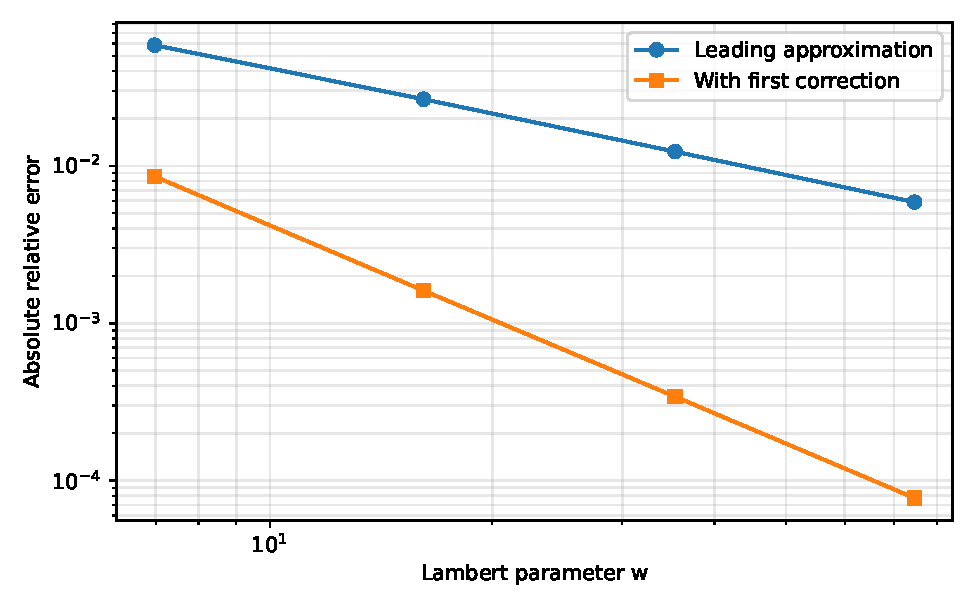
\includegraphics[width=0.87\textwidth]{figures/nd_saddle_errors.pdf}
\caption{Absolute relative errors for the data in Table~\ref{nd:tab:saddle}.
The first correction improves the observed error from the scale \(1/w\)
to the scale \(1/w^2\), as predicted by the theorem. The graph is a numerical
check, not a uniform error bound.}
\label{nd:fig:saddle}
\end{figure}

\section{The diagonal boundary layer}
For \(z=q=\e^{-t}\), direct logarithmic-product evaluation gives
Table~\ref{nd:tab:boundary}. The signs of the errors need not be monotone; the
statement is a superalgebraic bound, not monotone convergence of the error.

\begin{table}[htbp]
\centering
\caption{The joint endpoint \(\Phi_q(q)\to1/\sqrt2\). Values are rounded;
the full data are in \texttt{boundary\_layer.csv}.}
\label{nd:tab:boundary}
\begin{tabular}{@{}rrr@{}}
\toprule
\(t\)&\(\Phi_{\e^{-t}}(\e^{-t})\)&Error from \(1/\sqrt2\)\\
\midrule
1&0.758123053523105&\(5.1016\cdot10^{-2}\)\\
0.5&0.710249881663610&\(3.1431\cdot10^{-3}\)\\
0.25&0.706267615662706&\(-8.3917\cdot10^{-4}\)\\
0.125&0.707016842592727&\(-8.9939\cdot10^{-5}\)\\
0.0625&0.707106345877474&\(-4.3531\cdot10^{-7}\)\\
\bottomrule
\end{tabular}
\end{table}
% ---- ND lines 1818--1911 ----
\chapter{Further deductions, limitations, and research directions}
\label{nd:sec:frontiers}

\section{A unifying finite--infinite correspondence}
There are three distinct forms of compression in the proved results.
In the correlation problem, all interactions with a dyadic boundary are
compressed into the integer \(D(\bm h)\). In the nonlinear moment problem,
all Boolean cancellations are compressed into the covering condition
\(\bigcup\CCov=V\). In the product problem, the exact dyadic scaling is
compressed into the periodic amplitude \(\Psi\), while the continuous part
is handled by one saddle.

The comparison is structural, not an assertion that the three formulas are
special cases of a single theorem already proved here. Their common feature
is that cancellation is dealt with \emph{before} taking the asymptotic limit.
Doing the reverse can lose the boundary term, misidentify the first surviving
moment, or retain the wrong index in an infinite sum.

\section{Classifying vanishing boundary functionals}
\begin{question}
Which tuples \(\bm h\), modulo translations and deletion of repeated pairs,
satisfy \(D(\bm h)=0\)? Can their binary structure be characterized without
explicitly summing \eqref{nd:eq:defect}?
\end{question}

For even order, \(D=0\) means every sufficiently large dyadic cyclic and
noncyclic sum equals its mean times the block length exactly. For odd order,
it means every sufficiently large aligned dyadic block sum is zero. This is
a finite classification problem with a precise observable consequence.
The pair recurrence \eqref{nd:eq:Drec} provides a starting model, but the
higher-order combinatorics of the threshold parities \(b_t\) are richer.
No classification is claimed in this part.

\section{Designed nonlinear cancellation beyond a hafnian}
\begin{question}
For a prescribed sparse interaction graph, what is the largest possible
vanishing order of \(Z_x(t)\) among nontrivial signed quadratic weights,
subject to chosen normalization constraints on the linear part?
\end{question}

The positive-weight answer is determined by the minimum cover. Signed weights
allow algebraic cancellation among minimum covers, so the problem becomes a
finite polynomial system built from \eqref{nd:eq:allmoments}. Useful constraints
would exclude degenerate choices that make \(x\) independent of a bit and
force \(Z_x\equiv0\). Requiring the coordinate map to be injective on the
Boolean cube is another natural way to rule out trivial pairwise coincidences.
The part supplies the equations but does not assert an optimal solution.

\section{Uniform matching of the two analytic regimes}
The fixed-\(z\) saddle corresponds to \(\beta=-\log z\) bounded away from zero,
while the boundary layer has \(\beta=\gamma t\). The intermediate regime
\(t\ll\beta\ll1\) should connect the large-\(\gamma\) asymptotics of
\(\mathcal H(\gamma)\) with the moving discrete saddle. A rigorous uniform
formula would need to control the relation between saddle width and mesh
size throughout that transition. Theorems~\ref{nd:thm:saddle} and
\ref{nd:thm:boundarylayer} establish the two endpoints but do not prove the full
uniform bridge.

\begin{question}
Can one construct a single asymptotic approximation, with an explicit
uniform remainder, valid when \(\beta/t\to\infty\) while \(\beta\to0\),
and matching both \eqref{nd:eq:fullsaddle} and \eqref{nd:eq:boundaryF}?
\end{question}

This is a concrete continuation problem rather than a request to speculate
about a nonexistent singularity. The exact positive representation
\eqref{nd:eq:F} and the amplitude identity \eqref{nd:eq:Afactor} remain valid
throughout the real parameter region and provide the required starting point.

\section{Beyond-all-orders corrections and complex parameters}
The saddle theorem suppresses lattice effects beyond every algebraic order
in \(1/w\). The boundary-layer theorem suppresses all Euler summation powers
of \(t\). Identifying the leading remaining corrections would require more
than extending the coefficient list: one must study the analytic continuation
of the amplitude and the relevant complex saddles or Fourier modes.
That problem is a natural transseries extension, but it is not solved by the
present all-order Poincar\'e expansion. Similarly, \(|z|=1\) is a boundary of
the absolute convergence arguments, and root-of-unity specialization requires
a fresh proof.

\section{Possible formalization targets}
The finite correlation and covering theorems have a relatively direct route
to formal proof: finite sums, bit decompositions, parity, and Boolean monomial
identities suffice. An initial formalization could isolate
\eqref{nd:eq:blockfactor}, \eqref{nd:eq:Vm}, and \eqref{nd:eq:cover}, then derive the
remaining finite identities as corollaries. Such a project should use the
actual theorem names and conventions of the current repository after a
separate code audit; none are invented here.

The analytic results require additional infrastructure for infinite products,
termwise differentiation, dominated convergence, and uniform saddle estimates.
They should not be marked formalized merely because their numerical checks
pass. The supplied Python code is reproducibility material, not a proof
assistant certificate.
% ---- hand chunk 60-appendix-head.tex ----

\appendix

% ---- BC lines 1588--1608 ----
\chapter{Compact formula sheet for Part I}
\label{bc:app:formula}
With $N=2^m$, $g(k)=B_k(-2)$, and $\mathcal Q(z)=zE(z)^2$, the central formulas are
\begin{align*}
 r_m(k)-\eta(k)&=\frac{(-1)^m}{3N}g(k),&&0\le k\le N,\\
 A_m(k)-N\eta(k)&=-\frac23(-1)^mg(k),&&0\le k\le N,\\
 \mt_m&=(\mu_m+2\mu_{m+1})/3,&
 \ft_m&=f_m(1-\tfrac23\cos(2\pi Nx)),\\
 \widehat{\mt_m}(k)&=\eta(k),&&|k|\le N,\\
 \widehat\nu(k)&=g(|k|)/3,&&k\ne0,\\
 \mathcal G_m-\mathcal G&=\frac{(-1)^m}{3N}\mathcal Q(z)\mathcal K(z^N),&&|z|<1,\\
 2\mathcal K(z)+\mathcal K(z^2)&=3E(z)^{-2},&\mathcal K(0)&=1,\\
 \kappa_n&=\frac32\sum_{j=0}^{\vnu(n)}(-1/2)^jp_2(n/2^j),&&n\ge1.
\end{align*}
The exponents are
\[
 \sigma=\frac12\log_2\frac{1+\sqrt{17}}4,\qquad s_*=1+\sigma.
\]
The raw Sobolev rate is $N^{\sigma-s}$ below $s_*$, $N^{-1}\sqrt{\log N}$ at
$s_*$, and $N^{-1}$ above it. The corrected rate is $N^{\sigma-s}$ throughout
$s>\sigma$. Every use of these rates fixes $s$ before taking $N\to\infty$.
% ---- hand chunk 61-app-dc-head.tex ----

\chapter{Coefficient register and normalization checks for Part II}
\label{dc:app:coefficients}

% ---- DC lines 2083--2132 ----
The first six coefficients in the centered expansion are
\begin{center}\small
\begin{tabular}{@{}cl@{}}
\toprule
$r$&$A_r$ in $\calH(x)\sim\sum_{r\ge0}(-1)^rA_rx^r$\\
\midrule
0&$1$\\[2pt]
1&$1/9$\\[2pt]
2&$248/2025$\\[2pt]
3&$4806656/2679075$\\[2pt]
4&$3993751257088/10247461875$\\[2pt]
5&$454890030220640780288/345944065438125$\\
\bottomrule
\end{tabular}
\end{center}
All are obtained by the finite formula \cref{dc:eq:c-finite} followed
by multiplication by $2^{2r^2+r}$. Their rapid growth is predicted
by \cref{dc:thm:c-asymptotic}; it is not numerical instability.

The following identities are convenient independent checks:
\begin{align*}
 &\Phi(0)=1,\quad \Phi'(0)=-\tfrac12,\quad
    [z^2]\log\Phi(z)=\tfrac1{72},\\
 &K(2t)t=K(t),\quad C(1)=2C_0,\quad C(-1)=C_0,\\
 &\E T^2=8,\quad \E W=\tfrac1{72},\quad
    \E(T^2W)=\tfrac19,\\
 &Z_m(1/2)=C_0\,2^{m(m-1)/2}\calH(4^{-m}),\\
 &D(s,1/2)=(1+2^s)D(s,1).
\end{align*}
There is also an exact normalization check at $m=0$:
\[
 Z_0(1/2)=L,\qquad Z_0(1)=L/2,\qquad C_0\calH(1)=L.
\]
Indeed, $P(2u)-P(u)=e^{-u}P(2u)$, so substitution $t=2u$ gives
\[
 M(0,1/2)=\int_0^\infty\frac{P(2u)-P(u)}u\dd u=L.
\]
To justify the last equality without splitting divergent integrals,
integrate first over $[\epsilon,R]$. The difference is
$\int_R^{2R}P(u)\dd u/u-\int_\epsilon^{2\epsilon}P(u)\dd u/u$;
use $P(\infty)=1$ and $P(0)=0$. Differentiating
\cref{dc:eq:half-one} at zero gives the value at $a=1$.
These are classical product-normalization consequences, recorded
here as checks rather than new evaluations.

A sign error in the logarithmic centering changes the odd
coefficients; a missing factor of $2$ in the Mellin scaling changes
the moment law; and confusing $\Psi(z)$ with $\Psi(\sqrt z)$ changes
the optimal truncation scale. Each of these errors is detected by
at least one of the checks above.
% ---- hand chunk 62-app-dc-alpha-head.tex ----

\section{A direct nonrecursive formula for every asymptotic coefficient}
\label{dc:app:alpha}

% ---- DC lines 2135--2154 ----
For readers wishing to implement the general-shift expansion without
Bell-polynomial conventions, define $b=1/2-a$ and
\[
 d_r=-\frac{B_{2r}}{2r(2r)!(2^{2r}-1)}.
\]
Then its coefficient $\alpha_j(a)=2^{j(j+1)/2}\beta_j(a)$ is
\begin{equation}
 \boxed{\displaystyle
 \alpha_j(a)=2^{j(j+1)/2}
 \sum_{\substack{n_0,n_1,\ldots,n_{\lfloor j/2\rfloor}\ge0\\
 n_0+2n_1+4n_2+\cdots+2\lfloor j/2\rfloor n_{\lfloor j/2\rfloor}=j}}
 \frac{b^{n_0}}{n_0!}
 \prod_{r=1}^{\lfloor j/2\rfloor}\frac{d_r^{n_r}}{n_r!}.}
 \label{dc:eq:alpha-final}
\end{equation}
The sum is finite. At $b=0$, only even $j=2r$ survive, and
$\alpha_{2r}(1/2)=(-1)^rA_r$. For the complex translated expansion,
simply multiply its $j$th coefficient by $2^{js}$ before multiplying
by $C(s)$. Thus a single finite coefficient formula covers both the
real-zero slopes and the complex zero-string expansion.
% ---- RR lines 1319--1370 ----
\chapter{Finite formulas for every coefficient of Part III}
\label{rr:app:finite}

The part uses Bell polynomials, Bernoulli numbers, and rational negative-index polylogarithms as convenient names. This appendix makes explicit that no hidden recurrence is required.

\section{Eulerian coefficients and rational polylogarithms}
For integers \(m\geq1\), \(0\leq j<m\), define
\begin{equation}
 A(m,j)=\sum_{\ell=0}^{j+1}(-1)^\ell
                    \binom{m+1}{\ell}(j+1-\ell)^m.
 \label{rr:eq:Eulerianfinite}
\end{equation}
Then, for \(n\geq2\),
\begin{equation}
 \Li_{1-n}(w)=
 \frac{\displaystyle\sum_{j=0}^{n-2}A(n-1,j)w^{j+1}}{(1-w)^n},
 \qquad \Li_0(w)=\frac{w}{1-w}.
 \label{rr:eq:Lifinite}
\end{equation}
To prove this, begin in \(|w|<1\), where repeated application of \(w\dd/\dd w\) gives \(\Li_{-m}(w)=\sum_{k\geq1}k^mw^k\). Multiplication by \((1-w)^{m+1}\) produces exactly the coefficients in \eqref{rr:eq:Eulerianfinite}. Coefficients beyond degree \(m\) vanish by the \((m+1)\)-st finite difference of a degree-\(m\) polynomial. Both sides are rational functions, so the identity extends to every \(w\ne1\).

\section{Bernoulli numbers without a recurrence}
With the convention \(B_1=-1/2\), one has
\begin{equation}
 B_n=\sum_{k=0}^n\frac1{k+1}\sum_{j=0}^k(-1)^j\binom{k}{j}j^n.
 \label{rr:eq:Bernoullifinite}
\end{equation}
The convention \(0^0=1\) applies. Indeed, as a formal power series,
\[
 \sum_{k\geq0}\frac{(1-\e^z)^k}{k+1}
 =\frac{-\log(1-(1-\e^z))}{1-\e^z}
 =\frac{z}{\e^z-1}.
\]
For the coefficient of \(z^n\), only \(k\leq n\) contributes. Expanding the finite binomial sum proves \eqref{rr:eq:Bernoullifinite}. Use \(\beta_1=1/2\), \(\beta_n=B_n/n\) for \(n\geq2\), as in the main text.

\section{Bell coefficients as constrained finite sums}
For any cumulant list \(x_1,\ldots,x_h\),
\begin{equation}
 \B_h(x_1,\ldots,x_h)
 =h!\sum_{\substack{\nu_1,\ldots,\nu_h\geq0\\
                         \nu_1+2\nu_2+\cdots+h\nu_h=h}}
         \prod_{j=1}^h\frac1{\nu_j!}
                              \left(\frac{x_j}{j!}\right)^{\nu_j}.
 \label{rr:eq:Bellfiniteappendix}
\end{equation}
This follows directly by multiplying the exponential series
\(\prod_{j\geq1}\exp(x_jz^j/j!)\) and extracting the coefficient of \(z^h\). Inserting \eqref{rr:eq:Lifinite}, \eqref{rr:eq:Bernoullifinite}, and the finite cycle sums into \eqref{rr:eq:Bellfiniteappendix} gives literal nested finite sums for every moment and every correction coefficient appearing in the part.

\chapter{Normalization and logical checkpoints for Part III}
The main identities are sensitive to four conventions. First, \(P_m\) has \(m\) factors and \(2^m\) coefficients; \(P_0=1\). Second, the local window is \(\zeta\e^{z/2^m}\), not \(\zeta\e^{z/2^{m+1}}\). Third, \(\Up\) is the transform of \(X\in[0,1]\), with mean \(1/2\), rather than of its centered or rescaled Rvachev version. Finally, Bell polynomials encode exponential generating coefficients, so the factors \(h!\) and \((M+h)!/h!\) cannot be omitted.

There are also three logical distinctions worth retaining. An entire quotient formula is interpreted through a denominator-free identity or a proved removable continuation. Fourier nondecay does not, on its own, prove pure singularity; the orbit-average argument supplies that missing step. And an analytic Gaussian limit does not imply that the finite complex approximants are probability transforms. These distinctions keep the algebraic, analytic, and probabilistic claims aligned.
% ---- RS lines 1767--1808 ----
\chapter{Normalization dictionary and implementation details for Part IV}\label{rs:app:normalization}

\section{Frequency conventions}

The angular-frequency transform used here is $\widehat u(t)$ in
\eqref{rs:eq:Q}. Under the cyclic-frequency convention
$\widehat u_{\mathrm c}(\xi)=\int e^{-2\pi\ii\xi x}u(x)\dd x$, evenness gives
\begin{equation}
 \widehat u_{\mathrm c}(\xi)=\widehat u(2\pi\xi)
   =\prod_{j=0}^{\infty}\sinc(\pi\xi/2^j).
 \label{rs:eq:cyclic-frequency}
\end{equation}
A finite cyclic product indexed $j=0,\ldots,n$ therefore corresponds
to the spline $u_{n+1}$ in this part. Its omitted-tail scale is
$2^{-(n+1)}$, not $2^{-n}$. The even moments of its normalized
cyclic-frequency energy measure are
\begin{equation}
 (2\pi)^{-2r}2^{r(r+1)}.
\end{equation}
This dictionary is important when comparing formulas with
repository documents that use a different Fourier convention or
start their product index at zero.

\section{Integer-only evaluation of a spline derivative}

For $x=a/b$ with $b>0$ and $p=m-1-r\geq1$, put
\begin{equation}
 T=a2^m+b(2^m-1).
\end{equation}
Then \eqref{rs:eq:spline-deriv-positive} is
\begin{equation}
 u_m^{(r)}(a/b)
 =\frac{2^{m(m-1)/2}}{p!(b2^m)^p}
       \sum_{\substack{0\leq n<2^m\\T-2bn>0}}
           \eps_n(T-2bn)^p.
 \label{rs:eq:integer-spline-evaluation}
\end{equation}
The sum is an integer and can be accumulated before one final
rational division. For a highest cellwise derivative, $p=0$,
use the same formula away from knots with the positive-part
indicator convention. The supplied implementation treats values
outside the support as zero before forming the signed sum.
% ---- RS lines 1826--1861 ----
\chapter{Statement ledger for Part IV}\label{rs:app:ledger}

\begin{longtable}{@{}p{0.26\textwidth}p{0.67\textwidth}@{}}
\toprule
Result & Precisely what is established\\
\midrule
\endhead
Global correction &
\Cref{rs:thm:global,rs:thm:sharp,rs:cor:holder}: all fixed orders, global
classical and H\"older norms, explicit constants, and sharp leading
supremum asymptotics.\\[4pt]
Increasing order &
\Cref{rs:cor:growing}: a supergeometric absolute error certificate
with a specified admissible order; no relative endpoint or
numerical-conditioning claim.\\[4pt]
Dyadic splines &
\Cref{rs:thm:dyadic,rs:cor:exact-degree,rs:thm:richardson}: exact polynomial
stabilization, exact degree in lowest terms, finite extraction,
and an order-independent absolute amplification bound.\\[4pt]
Discrete array &
\Cref{rs:thm:lattice-operator,rs:thm:local-limit,rs:thm:dyadic-lattice}:
finite differential conversion, a uniform all-orders local-limit
bound, and exact stopping on fixed dyadic odd-level subsequences.\\[4pt]
Energy moments &
\Cref{rs:thm:energy-moments,rs:thm:lognormal,rs:thm:theta}: exact moments,
explicit distinct continuous and atomic moment twins, and hence
moment indeterminacy.\\[4pt]
Geometric extension &
\Cref{rs:thm:geometric}: exact separated-copy norms and the resulting
moment class for $0<\theta\leq1/2$, not for overlapping copies.\\[4pt]
Priority and verification &
Proofs and finite exact computations are supplied; universal
publication priority, peer review, and Lean formalization are
not claimed.\\
\bottomrule
\end{longtable}
% ---- ND lines 1931--2006 ----
\chapter{Coefficient generation without hidden recurrences for Part V}
\label{nd:app:coefficients}

For a requested saddle order \(n\), formula \eqref{nd:eq:cn} is a finite weighted
partition sum. An implementation can loop over \(k_j\) with
\(0\le k_j\le\lfloor2n/(j-2)\rfloor\), discard assignments for which
\(\sum(j-2)k_j>2n\), and set
\(\ell=2n-\sum(j-2)k_j\). This directly generates the coefficient in the
formal symbols \(A_0,\ldots,A_{2n}\). The program's recursive enumeration is
only a traversal of this finite index set; the mathematical coefficient formula
does not depend on previously computed coefficients.

The derivatives \(A_j\) can themselves be expressed as finite combinations of
\(\Psi^{(r)}(\theta)\). Let \(s=\log y\) and
\[
 B_\theta(s)=\e^{-s^2/(2a)}\Psi(\theta-s/a).
\]
Since \(\dd/\dd y=\e^{-s}\dd/\dd s\), induction gives
\begin{equation}
 \mathcal A_\theta^{(\ell)}(1)
 =\left.\left(\prod_{j=0}^{\ell-1}(D_s-j)\right)
                            B_\theta(s)\right|_{s=0},
 \qquad D_s=\frac{\dd}{\dd s}.
 \label{nd:eq:Aoperator}
\end{equation}
For \(\ell=0\), the empty operator product is the identity. To prove the
formula, write
\(\dd^\ell/\dd y^\ell=\e^{-\ell s}\prod_{j=0}^{\ell-1}(D_s-j)\)
and differentiate once more; the derivative of \(\e^{-\ell s}\) introduces
the next factor \(D_s-\ell\).

If \(s(\ell,j)\) denotes the signed Stirling coefficient defined by
\(u(u-1)\cdots(u-\ell+1)=\sum_js(\ell,j)u^j\), then
\begin{equation}
 \mathcal A_\theta^{(\ell)}(1)
 =\sum_{j=0}^{\ell}s(\ell,j)
   \sum_{h=0}^{\lfloor j/2\rfloor}
       \frac{j!}{h!(j-2h)!}
       \left(-\frac1{2a}\right)^h
       \left(-\frac1a\right)^{j-2h}
       \Psi^{(j-2h)}(\theta).
 \label{nd:eq:Astirling}
\end{equation}
Indeed, expand the Gaussian factor in even powers of \(s\), expand the
translated \(\Psi\) by its finite derivative coefficient, and extract the
\(j\)-th derivative at zero. Substituting \eqref{nd:eq:Astirling} into
\eqref{nd:eq:cn} produces a fully explicit finite formula for each saddle
coefficient in the derivatives of the periodic function.

\chapter{Notation and normalization reference for Part V}
\begin{longtable}{@{}p{0.23\textwidth}p{0.72\textwidth}@{}}
\toprule
Symbol&Meaning\\
\midrule
\endhead
\(\eps_n\)&The sign \((-1)^{s_2(n)}\), with \(\eps_0=1\).\\[2mm]
\(E(z)\)&The ordinary generating function \(\sum_{n\ge0}\eps_nz^n\).\\[2mm]
\(\bm h,H,p\)&A shift tuple with minimum zero, its maximum, and its length.\\[2mm]
\(D(\bm h)\)&The integer boundary functional in \eqref{nd:eq:defect}.\\[2mm]
\(S_m,R_m\)&Noncyclic and cyclic sums over a block of length \(2^m\).\\[2mm]
\(\sigma(\Phi)\)&The alternating binary digit sum, not the ordinary digit sum.\\[2mm]
\(Z_x(t)\)&The signed exponential sum on a nonlinearly positioned Boolean cube.\\[2mm]
\(\HH,\tau\)&The family of nonempty monomial supports and its minimum cover size.\\[2mm]
\(\Haf(J)\)&The sum of products over perfect matchings; no determinant signs.\\[2mm]
\(\MM_G\)&The weighted matching polynomial, including unmatched singleton weights.\\[2mm]
\(\Phi_q(z)\)&The geometric product \(\prod_{j\ge0}(1-zq^j)^{\eps_j}\).\\[2mm]
\(P(x)\)&The positive product \(E(\e^{-x})\).\\[2mm]
\(\Phi(x)\)&The Laplace transform of \(\sum_{k\ge1}2^{-k}U_k\), with \(U_k\) uniform on \([0,1]\).\\[2mm]
\(\Psi(v)\)&The positive one-periodic function in \eqref{nd:eq:Psidef}.\\[2mm]
\(F(t,z)\)&The positive logarithmic deviation \(-\log\Phi_{\e^{-t}}(z)\) for real positive \(z\).\\[2mm]
\(a,\beta,\Lsad\)&Respectively \(\log2\), \(-\log z\), and \(\log(1/t)\).\\[2mm]
\(w,r_*,\theta\)&The Lambert parameter, saddle location, and periodic phase in \eqref{nd:eq:saddleparams}.\\[2mm]
\(\Pi(t,z),c_n\)&The saddle prefactor and its periodic coefficient functions.\\[2mm]
\(\mathcal H,\mathcal P\)&The joint-endpoint integral and its exponential, distinct from the saddle prefactor \(\Pi(t,z)\).\\
\bottomrule
\end{longtable}
% ---- hand chunk 70-provenance.tex ----

\chapter{Source provenance, notation dictionary, and reproducibility}
\label{app:provenance}
\section{Sources and consolidation}
This volume consolidates the six Thue--Morse reports filed in the
repository's frontier intake of September 4, 2026, under
\path{drafts/thue-morse/}: \path{Thue_Morse_Boundary_Corrections},
\path{Thue_Morse_Dyadic_Completion}, \path{thue_morse_research_article}
(\emph{Thue--Morse Mellin Renormalization and Gamma-Tower Uniqueness}),
\path{Thue_Morse_Rational_Resonances}, \path{Thue_Morse_Research}
(\emph{New Deductions from Thue--Morse Cancellation}), and
\path{Thue_Morse_New_Directions}. Their \LaTeX{} sources, PDFs, READMEs and
audit notes were removed when this volume was filed; the repository history
retains them. The verification programs, their recorded outputs, the
figures, and the generated table were retained unchanged.

The correspondence between sources and parts is as follows. Part I is the
boundary-corrections article, with the correlation chapter of the
new-directions article appended, since its pair case is the Stern boundary
term. Part II merges the dyadic-completion article (its spine) with the
Mellin-renormalization article: the completion, its Mellin transform and
periodic factor, the Dirichlet continuation, the real zeros and their
slopes, the rescaling identity, the coefficient formulas, and the moment
twins were proved in both; the first article's versions were kept because
they carried the more complete proofs (the boundary argument for the
nonconstancy of the profile, the zero-free periodic lemma, the Gaussian
localization), and the second article's contributions were added where they
went further: the uniform theorem with an explicit tube constant
(\cref{ra:sec:asymptotics}), the real-order slopes and their dyadic
equation, the Hankel growth (\cref{ra:sec:moments}), the classification of
completely monotone dyadic solutions, the universal coefficients and the
beyond-all-orders ambiguity, the boundary uniqueness and the gamma-tower
characterization, and the independent numerical evaluation. Part III is the
rational-resonances article, Part IV the new-deductions article, and Part V
the remaining chapters of the new-directions article. The preliminaries
that all six sources restated (the signed sequence, the finite product, the
generating function, Prouhet cancellation, the Laplace product with its
flatness, the uniform-sum variable with its transform, its zeros and its
Fabius functional equation, the Bernoulli expansions, and the Bell and
partition polynomials) are stated once in \cref{ch:prelim}; the sources'
own versions were removed and their references redirected.

Before deduplicating, the following identifications were checked: the two
completions $K=P\Phi$ and $W=QH$ are the same function, with the same
dilation law, profile and Mellin shift; the two coefficient families
$\beta_j(a)$ and $r_k(a)$ agree, as do $\alpha_j=2^{j(j+1)/2}\beta_j$ and
$c_k$ once the sign of $b=1/2-a$ is aligned; the centered expansions agree
term by term ($1/9$, $248/2025$, $4806656/2679075$); the slopes
$Z_m(a)=M(-m,a)$ and $C_m(a)$ are the same integrals; the normalization
constants $C_0=K_0=0.75072198040787\ldots$ agree in both reports' runs; the
entire-order theorem was proved in both and kept once; and the pair boundary
functional $D(0,h)$ of the correlation chapter is the Stern value
$g(h)=B_h(-2)$ of Part I. No discrepancy was found.

\section{Notation dictionary for the merged part}
The merged Part II uses the first source's letters. The second source's
letters, which appear in its retained verifier and its data files, are:
\begin{center}\small
\begin{tabular}{@{}lll@{}}
\toprule
This volume & Mellin-renormalization report & Meaning\\
\midrule
$P(t)$ & $Q(t)$ & the Laplace product $\prod_j(1-e^{-2^jt})$\\
$\Phi(z)$ & $H(z)$ & the Fabius transform $\E e^{-zX}$\\
$K(t)$ & $\mathcal W(t)$ & the completion $P\Phi$\\
$C(s)$, $C_0$ & $K(s)$, $K_0$ & the Mellin transform of $K$ and its value at $0$\\
$H(Lv)$, $h_k$ & $A(v)$, $a_k$ & the periodic profile and its Fourier coefficients\\
$h_\pm$ & $A_\pm$ & its bounds\\
$L$ & $\lambda$ & $\log2$\\
$Z_\rho(a)$ & $C_\rho(a)$ & the slope $M(-\rho,a)$\\
$B_a(z)$, $\beta_k(a)$ & $R_a(z)$, $r_k(a)$ & the reciprocal transform and its coefficients\\
$\alpha_k(a)$ & $c_k(a)$ & $2^{k(k+1)/2}\beta_k(a)$\\
$b=1/2-a$ & $b=a-1/2$ & the centering parameter (odd coefficients change sign)\\
$\calH(4^{-m})$ & $Z_m$ & the normalized centered slope\\
$\Theta(\rho)=C_0Q(-\rho)$ & $\Theta(\rho)$ & the real-order periodic amplitude\\
\bottomrule
\end{tabular}
\end{center}
In Part I the letters $K$, $H$, $Q$ of the boundary-corrections report were
changed to $\mathcal K$, $\mathcal G$, $\mathcal Q$ to keep them distinct
from Part II's, and its unit disk $\mathbb D$ is written out. In Part IV the
sinc product $Q(t)$ of the new-deductions report is written $\widehat u(t)$,
the transform of the up-function. In Part V the letters $A$, $Q$, $B$,
$P(t,z)$, $L$ of the new-directions report are $P$, $\Phi$, $K$, $\Pi(t,z)$,
$\Lsad$, so that its product, Laplace transform and completion are visibly
those of \cref{ch:prelim} and Part II; its periodic amplitude satisfies
$\Psi(v)=H(-av)$. Everything else keeps its source notation, listed in
\cref{sec:dictionary}.

\section{Retained verification programs}
The six programs live under \path{verification/} in the package directory,
unchanged, with the outputs of the runs the sources recorded:
\begin{itemize}
\item \path{source1/} (Part I): \path{verify.py}, standard library only,
$19{,}037$ exact rational checks recorded in \path{verification.json};
\path{make_figures.py} and \path{poisson_data.json} regenerate the figures
and the Poisson table (\path{tables/bc_poisson_table.tex}) with
\texttt{mpmath}, \texttt{numpy} and \texttt{matplotlib}.
\item \path{source2/} (Part II, dyadic completion): \path{code/verify.py}
and \path{code/check_original_mellin.py} with \path{code/requirements.txt};
outputs in \path{data/} at 60 and 80 digits, including the completion
constant and the displayed zero.
\item \path{source3/} (Part II, Mellin renormalization):
\path{verify_results.py} with \texttt{mpmath} and \texttt{sympy};
\path{results_48.json} and \path{results_80.json}.
\item \path{source4/} (Part III): \path{verify.py} working in
$\Q[x]/\Phi_q(x)$; \path{requirements.txt}; \path{results/} with the
verification report and the four error tables.
\item \path{source5/} (Part IV): \path{verify.py}, standard library only,
$3{,}796$ exact checks recorded in \path{verification_results.json}.
\item \path{source6/} (Parts I and V): \path{verify.py} with \texttt{mpmath}
and \texttt{sympy}; \path{verification_results.json},
\path{verification_run.txt}, the four CSV tables and \path{environment.json}.
\end{itemize}
Each is run with \texttt{python} from inside its directory as its part's
verification section describes. The programs recompute their certificates;
they do not read the saved reports. They are finite checks of the
implementation and formulas, not replacements for the proofs.

\section{Formalization status}
No Lean files were added or compiled for this volume. Each part ends with
the formalization route its source proposed; the atlas names the modules
(\path{ThueMorseBoundaryFlatness.lean}, \path{ThueMorseEntireContinuation.lean},
and the finite-product bridges) on which such work would build.

\section{Files and commands}
The package directory contains \path{Thue_Morse_Frontier_Deductions.tex},
its compiled PDF, \path{README.md}, \path{figures/}, \path{tables/}, and
\path{verification/}. The volume loads \path{docs/fabius-notation.tex} by
relative path; with a \TeX{} installation containing Libertinus (or, as a
fallback, Latin Modern) and the listed standard packages, compile with three
passes of
\begin{verbatim}
pdflatex -interaction=nonstopmode -halt-on-error \
  Thue_Morse_Frontier_Deductions.tex
\end{verbatim}

% ---- hand chunk 71-bibliography.tex ----

\backmatter
\begin{thebibliography}{99}
\addcontentsline{toc}{chapter}{Bibliography}

\bibitem{atlas}
Vladimir Reshetnikov, \emph{The Thue--Morse Sequence: Formula Atlas and
Fabius--Rvachev Frontier Results}, consolidated August 28, 2026, ProveIt
repository. Sources consulted September 4, 2026.
\url{https://github.com/VladimirReshetnikov/ProveIt/tree/main/Analysis/FabiusFunction/docs/semi-formalized-research-frontiers/drafts/thue-morse/Thue_Morse_Atlas_and_Frontiers}.

\bibitem{aguech-jedidi}
R.~Aguech and W.~Jedidi, ``New characterizations of completely monotone
functions and Bernstein functions, a converse to Hausdorff's moment
characterization theorem,'' \emph{Arab Journal of Mathematical Sciences}
\textbf{25} (2019), 57--82.

\bibitem{agk}
R.~Arratia, L.~Goldstein, and F.~Kochman, ``Size bias for one and all,''
\emph{Probability Surveys} \textbf{16} (2019), 1--61, especially Section 9.
\url{https://doi.org/10.1214/13-PS221}.

\bibitem{alkauskas}
G.~Alkauskas, \emph{Dirichlet series associated with the Thue--Morse
sequence}, Vilnius University preprint 2001-15 (2001). Bibliographical
reference only: the full text was not retrieved by either source that cites
it. \url{https://web.vu.lt/mif/g.alkauskas/math/index.html}.

\bibitem{allouche2015}
J.-P.~Allouche, ``Thue, combinatorics on words, and conjectures inspired by
the Thue--Morse sequence,'' \emph{Journal de Th\'eorie des Nombres de
Bordeaux} \textbf{27} (2015), 375--388; arXiv:1401.3727, Section 3.2.
\url{https://arxiv.org/abs/1401.3727}.

\bibitem{allouche-cohen}
J.-P.~Allouche and H.~Cohen, ``Dirichlet series and curious infinite
products,'' \emph{Bulletin of the London Mathematical Society} \textbf{17}
(1985), 531--538. \url{https://doi.org/10.1112/blms/17.6.531}.

\bibitem{allouche-shallit}
J.-P.~Allouche and J.~Shallit, ``The ubiquitous Prouhet--Thue--Morse
sequence,'' in C.~Ding, T.~Helleseth, and H.~Niederreiter (eds.),
\emph{Sequences and Their Applications}, Springer, 1999, pp.~1--16.
\url{https://cs.uwaterloo.ca/~shallit/Papers/ubiq15.pdf}.

\bibitem{amp}
J.-P.~Allouche, M.~Mend\`es France, and J.~Peyri\`ere, ``Automatic
Dirichlet series,'' \emph{Journal of Number Theory} \textbf{81} (2000),
359--373. \url{https://doi.org/10.1006/jnth.1999.2487}.

\bibitem{arias1982}
J.~Arias de Reyna, ``An infinitely differentiable function with compact
support: definition and properties,'' \emph{Revista de la Real Academia de
Ciencias Exactas, F\'isicas y Naturales de Madrid} \textbf{76} (1982),
21--38; English translation arXiv:1702.05442.

\bibitem{arias2018}
J.~Arias de Reyna, ``Arithmetic of the Fabius function,'' \emph{Integers}
\textbf{18} (2018), Paper A51.
\url{https://math.colgate.edu/~integers/s51/s51.pdf}.

\bibitem{ars}
J.-P.~Allouche, S.~Riasat, and J.~Shallit, ``More infinite products:
Thue--Morse and the gamma function,'' \emph{Ramanujan Journal} \textbf{49}
(2019), 115--128. \url{https://arxiv.org/abs/1709.03398}.

\bibitem{baake-coons}
M.~Baake and M.~Coons, ``Correlations of the Thue--Morse sequence,''
\emph{Indagationes Mathematicae} \textbf{35} (2024), 914--930.
\url{https://arxiv.org/abs/2209.07102}.

\bibitem{baake-grimm}
M.~Baake and U.~Grimm, ``The singular continuous diffraction measure of the
Thue--Morse chain,'' \emph{Journal of Physics A} \textbf{41} (2008), 422001.
\url{https://arxiv.org/abs/0809.0580}.

\bibitem{bolker}
E.~D.~Bolker, C.~Offner, R.~Richman, and C.~Zara, ``The
Prouhet--Tarry--Escott problem and generalized Thue--Morse sequences,''
\emph{Journal of Combinatorics} \textbf{7} (2016), 117--133.
\url{https://arxiv.org/abs/1304.6756}.

\bibitem{cloitre}
B.~Cloitre, \emph{The Thue--Morse transform}, arXiv:2604.06243v2 (May 2026).
Cited for related transform and Prouhet-partition context.
\url{https://arxiv.org/abs/2604.06243}.

\bibitem{cmps}
M.~Coons, J.~Maz\'a\v c, A.~Pincus--Kazmar, and A.~Stout, ``On the absolute
value of the autocorrelations of the Thue--Morse sequence,''
\emph{Experimental Mathematics}, published online January 31, 2026.
\url{https://arxiv.org/abs/2511.06386}.

\bibitem{dlmf413}
NIST Digital Library of Mathematical Functions, \S4.13, \emph{Lambert
$W$-function}. \url{https://dlmf.nist.gov/4.13}.

\bibitem{dlmf422}
NIST Digital Library of Mathematical Functions, \S4.22 and \S24.16,
infinite trigonometric products and generalized Bernoulli polynomials.
\url{https://dlmf.nist.gov/4.22}; \url{https://dlmf.nist.gov/24.16}.

\bibitem{duke}
W.~Duke and H.~N.~Nguyen, ``Infinite products of cyclotomic polynomials,''
\emph{Bulletin of the Australian Mathematical Society} \textbf{91} (2015),
400--411.

\bibitem{fabius}
J.~Fabius, ``A probabilistic example of a nowhere analytic
$C^\infty$-function,'' \emph{Zeitschrift f\"ur Wahrscheinlichkeitstheorie
und Verwandte Gebiete} \textbf{5} (1966), 173--174.

\bibitem{fgd}
P.~Flajolet, X.~Gourdon, and P.~Dumas, ``Mellin transforms and asymptotics:
harmonic sums,'' \emph{Theoretical Computer Science} \textbf{144} (1995),
3--58.

\bibitem{gohlke}
P.~Gohlke, M.~Kesseb\"ohmer, and T.~I.~Schindler, \emph{Generalized
Thue--Morse measures: spectral and fractal analysis}, arXiv:2509.22109
(2025).

\bibitem{haugland}
J.~K.~Haugland, \emph{Evaluating the Fabius function}, arXiv:1609.07999,
version 2 (2020).

\bibitem{heyde}
C.~C.~Heyde, ``On a property of the lognormal distribution,''
\emph{Journal of the Royal Statistical Society, Series B} \textbf{25} (1963),
392--393.

\bibitem{klavzar-stern}
S.~Klav\v zar, U.~Milutinovi\'c, and C.~Petr, ``Stern polynomials,''
\emph{Advances in Applied Mathematics} \textbf{39} (2007), 86--95.

\bibitem{li}
Y.-Q.~Li, \emph{Infinite products related to generalized Thue--Morse
sequences}, arXiv:2006.04187 (2020).

\bibitem{mmr}
C.~Mauduit, H.~L.~Montgomery, and J.~Rivat, ``Moments of a Thue--Morse
generating function,'' \emph{Journal d'Analyse Math\'ematique} \textbf{135}
(2018), 713--724.

\bibitem{sobolewski}
B.~Sobolewski, ``Cyclotomic properties of polynomials associated with
automatic sequences,'' \emph{Advances in Applied Mathematics} \textbf{120}
(2020), 102063. \url{https://arxiv.org/abs/1909.12052}.

\bibitem{toth}
L.~T\'oth, ``Linear combinations of Dirichlet series associated with the
Thue--Morse sequence,'' \emph{Integers} \textbf{22} (2022), A98.
\url{https://arxiv.org/abs/2211.13570}.

\bibitem{zaks}
M.~A.~Zaks, A.~S.~Pikovsky, and J.~Kurths, ``On the correlation dimension of
the spectral measure for the Thue--Morse sequence,'' \emph{Journal of
Statistical Physics} \textbf{88} (1997), 1387--1392.

\end{thebibliography}
\end{document}

